\documentclass{phdDissertation}

\usepackage{mathtools}
\usepackage{amsmath}
\usepackage{amssymb}
\usepackage{multicol}
\usepackage{multirow}
\usepackage{listings}
\usepackage{float}
\usepackage{empheq}
\usepackage{array}
\usepackage{datetime}
\usepackage{tabularx}

\newdateformat{monthyeardate}{\monthname[\THEMONTH], \THEYEAR}


\usepackage{placeins}
\let\Oldsection\section
\renewcommand{\section}{\FloatBarrier\Oldsection}
\let\Oldsubsection\subsection
\renewcommand{\subsection}{\FloatBarrier\Oldsubsection}


\usepackage{pgfplots}
\usepackage{graphicx}
\graphicspath{{logos/}}

\setcounter{tocdepth}{2}
\setcounter{secnumdepth}{3}

\usepackage[ruled]{algorithm2e}
\SetKw{KwStep}{step \hspace{1mm}}
\SetKw{KwFrom}{from}
\SetKw{KwAnd}{ and }
\SetKwFor{For}{For}{do}{End\hspace{1mm}for}
\SetKwFor{Par}{par}{do}{end\hspace{1mm}par}
\SetKwFor{ParFor}{For}{do in parallel}{End\hspace{1mm}parallel\hspace{1mm}for}
\SetKwIF{If}{ElseIf}{Else}{If}{then}{Else\hspace{1mm}if}{Else}{End\hspace{1mm}if}
\SetKwComment{tcn}{}{}

\usepackage[backend=bibtex,style=ieee,sorting=none]{biblatex}
\addbibresource{biblio}

\usepackage{hyperref}
\hypersetup{colorlinks=true,linkcolor=black,urlcolor=blue,citecolor=black}

\newcommand{\pluseq}{\mathrel{+}=}

\author{Jérôme Gurhem}

\labo{Centre de Recherche en Informatique, Signal et Automatique de Lille}
\doctoralschool{\large École doctorale Sciences Pour l'Ingénieur Université Lille Nord-de-France}
\dirname{Serge G. Petiton}
\locationsoutenance{Saclay}
\universitylogo{logos/logoLille.png}
\universitylogoscale{0.15}


\titleEN{Distributed and Parallel Programming Paradigms Using Graphs of Tasks for Post-Petascale Supercomputers}
\datesoutenanceEN{March 16h, 2021}
\specialiteEN{Computer Science}
\diraffiliationEN{University of Lille}

\juryEN{
\begin{tabular}{lll}
	Committee president & \quad William Jalby     & \quad Professor at University of Versailles Saint-Quentin-en-Yvelines \\
	\\
	Reporters           & \quad Michel Daydé      & \quad Professor at ENSEEIHT, France                                   \\
	                    & \quad Ewa Deelman       & \quad Professor at University of Southern California, USA             \\
	Examinators         & \quad Henri Calandra    & \quad Ph.D., Total SA, France                                         \\
	                    & \quad Barbara Chapman   & \quad Professor at University of Stony Brook,  USA                    \\
	                    & \quad Clarisse Dhaenens & \quad Professor at University of Lille, France                        \\
	                    & \quad Miwako Tsuji      & \quad Ph.D., RIKEN, Japan                                             \\
	Advisor             & \quad Serge G. Petiton  & \quad Professor at University of Lille, France
\end{tabular}
}

\titleFR{Paradigmes de Programmation Répartie et Parallèle Utilisant des Graphes de Tâches pour Supercalculateurs Post-Pétascale}
\datesoutenanceFR{16 mars 2021}
\specialiteFR{Informatique}
\diraffiliationFR{Université de Lille}


\juryFR{
\begin{tabular}{lll}
	Président du jury & \quad William Jalby     & \quad Professeur à l'Université Versailles Saint-Quentin-en-Yvelines \\
	\\
	Rapporteurs       & \quad Michel Daydé      & \quad Professeur à l'ENSEEIHT, France                                \\
	                  & \quad Ewa Deelman       & \quad Professeure à l’Université de Southern California, États-Unis  \\
	Examinateurs      & \quad Henri Calandra    & \quad Docteur, Total SA, France                                      \\
	                  & \quad Barbara Chapman   & \quad Professeure à l'Université de Stony Brook, États-Unis          \\
	                  & \quad Clarisse Dhaenens & \quad Professeure à l'Université de Lille, France                    \\
	                  & \quad Miwako Tsuji      & \quad Docteure, RIKEN, Japon                                         \\
	Directeur         & \quad Serge G. Petiton  & \quad Professeur à l'Université de Lille, France
\end{tabular}
}


\begin{document}

	\titlepage

	\chapter*{Acknowledgements}

Firstly, I would like to express my sincere gratitude to my advisors Prof. Serge G. Petiton and Dr. Henri Calandra for the continuous support of my Ph.D study and related research, for their patience, motivation, and immense knowledge.
Their guidance helped me during my research and the writing of this dissertation.
I could not have imagined having a better mentors for my Ph.D study.

I would like to thank Total SA for the funding that allowed me to conduct this thesis.

Besides my advisor, I would like to thank the rest of my thesis committee: Prof. William Jalby for presiding the committee, Prof. Michel Daydé, and Prof. Ewa Deelman for reviewing my Ph.D. dissertation, Prof. Barbara Chapman, Prof. Clarisse Dhaenens and Dr. Miwako Tsuji for participating in the committee,

I would like to thank all the members of the \textit{Maison de la Simulation} for welcoming me in the laboratory and for the stimulating discussions, especially Dr. Martial Mancip for his help with Docker and improving my Ph.D. defense.

My appreciation also goes out to my family and friends for their encouragement and support all through my studies.
I would also like to thank my girlfriend for her support in my work and every day life.

	\chapter*{Résumé}

Depuis le milieu des années 1990, les bibliothèques de transmission de messages sont les technologies les plus utilisées pour développer des applications parallèles et distribuées.
Des modèles de programmation basés sur des tâches peuvent être utilisés, par exemple, pour éviter les communications collectives sur toutes les ressources comme les réductions, les diffusions ou les rassemblements en les transformant en multiples opérations avec des tâches.
Ensuite, ces opérations peuvent être planifiées par l'ordonnanceur pour placer les données et les calculs de manière à optimiser et réduire les communications de données.

L'objectif principal de cette thèse est d'étudier ce que doit être la programmation basée sur des tâches pour des applications scientifiques et de proposer une spécification de cette programmation distribuée et parallèle, en expérimentant avec plusieurs représentations simplifiées d'applications scientifiques importantes pour TOTAL, et de méthodes linéaire classique dense et creuses.
Au cours de la thèse, plusieurs langages de programmation et paradigmes sont étudiés.
Des méthodes linéaires denses pour résoudre des systèmes linéaires, des séquences de produit matrice vecteur creux et la migration sismique en profondeur pré-empilement de Kirchhoff sont étudiées et implémentées en tant qu'applications basées sur des tâches.
Une taxonomie, basée sur plusieurs de ces langages et paradigmes est proposée.
Des logiciels ont été développés en utilisant ces modèles de programmation pour chaque application simplifiée.
À la suite de ces recherches, une méthodologie pour la programmation de tâches parallèles est proposée, optimisant les mouvements de données en général et, en particulier, pour des applications scientifiques ciblées.


	\chapter*{Abstract}

Nowadays, message passing libraries are the technology the most used to implement parallel and distributed applications.
However, they may not be a solution efficient enough on exascale machines since scalability issues will appear due to the increase in computing resources.
Task based programming models can be used to avoid collective communications like reductions, broadcast or gather by transforming them into multiple operations on tasks.
Then, these operations can be scheduled by the programming scheduler to place the data and computations in a way that optimize and reduce the data communications.
As programming models are evolving rapidly, it is important to have a clear view of the main capabilities of the current programming models in order to use the most suitable programming model to the targeted architectures and the implemented application.

The main objective of this thesis is to study what must be task-based programming for scientific applications and to propose a specification of such distributed and parallel programming, by experimenting for several simplified representations of important scientific applications for TOTAL.
The optimization of data movements will be studied and scheduling strategies proposed and evaluated.
During the dissertation, several programming languages and paradigms will be studied.
A detailed taxonomy of these will be proposed and a review of the developments in the field will be realized.
Software will be developed using these programming models for each simplified applications.
As a result of this research, a methodology for parallel task programming will be proposed, optimizing data movements, in general, and for targeted scientific applications, in particular.
A taxonomy of these languages and a strategy of evolution between the current codes and those respecting this methodology will be introduced.


	\tableofcontents
	\listoffigures
	\listoftables
	\lstlistoflistings

	\chapter{Introduction}

\section{Motivations}
Previously, the computing power of processors was mainly increasing with the frequency of the processors which cannot be increased easily anymore due the heat generation and the energy consumption increasing alongside.
Therefore, a major change in the architecture occurred in order to still increase the performances of the new supercomputers : more processors with tens of cores were introduced in supercomputers.
Moreover, graphic processing unit (GPU) also made their appearance in supercomputer nodes due to their high performances considering their low energy consumption compared to regular processes.
This leads to an increasing number of different architectures from which the users have to obtain performances.

Furthermore, in the recent massively parallel architectures, the users have to take advantage of multiple nodes constituted of several multi-core processors connected by network to achieve performance, which is done by implementing parallel applications.
Moreover, taking advantage of multiple nodes containing several multi-core processors involves the use of the network to send data from one node to another since the memory is local to the nodes.
Besides, new processors with a network on chip are also appearing on supercomputers like Fugaku A64FX CPUs and Sunway TaihuLight SW26010.
In these processors, the cores are not sharing the same memory.
Instead, there is a network that can be used to send data from one subset of core to the others.
These processors have hierarchical memory and network in which distributed memory is introduced at several level.
There is distributed memory at the level of supercomputer nodes and at the level of the groups of cores in the processor.

Nowadays, parallel and distributed applications are based on MPI+X where MPI is the Message Passing Interface \cite{MPIForum}, that is used to send the data between the nodes, and X is a parallel programming model that is used to take advantage of the computing resources of the nodes.
Usually, X may be OpenMP \cite{DaguM1998}, that takes advantage of shared memory and multi-threading to achieve performance on CPU and GPU and/or CUDA \cite{Shane2012}, that addresses parallelism on NVidia GPUs.
Applications can also implemented with pure MPI where MPI is used to spawn multiple processes on each node.
With the increase of available architectures (a combination of different generation of CPU and GPU), the portability of highly optimized applications for a given architecture is not assured on another architecture.
If the architecture is too different, it may also be possible that the application cannot be installed due to missing libraries dependent on a given architecture.

However, MPI may not be a solution efficient enough on exascale machines, especially in terms of fault tolerance and check-pointing \cite{SWAAB2014}.
Task-based approach can help in managing fault tolerance and check-pointing since the tasks could be restarted on another location and data from tasks saved at any moment.
Task based programming models can implement fault tolerance by restarting the failed tasks on other computing resources and even stop executing tasks on processors with high fault rate.
Check-pointing could be implemented by storing the state of the output of the task in a way that allow to restart the application at the last check-point and reconstruct the lost data.
Moreover, task based programming models can also be used to avoid collective communications like reductions, broadcast or gather by transforming them into multiple operations on tasks.
Then, these operations can be scheduled by the programming scheduler to place the data and computations in a way that optimize and reduce the data communications.
Therefore, with the merging of parallel and distributed programming, graph of tasks and efficient scheduler are a very interesting way to improve performances while reducing communications.
Schedulers that can optimize data migrations and task execution while keeping good performances are necessary.

While MPI focus on exchanging data between processes, other programming models may be efficient to parallelize applications with good scalability without being held back by global synchronizations.
For instance, Partitioned Global Address Space Languages (PGAS) programming models, that let the users see the distributed memory as a global memory address space that is partitioned across each processing element \cite{CDMCE2005}, are an alternative to MPI + X.
Task-based programming models, which allow to define fine-grain tasks (computations) on a specific set of data (input and output), are also an alternative to MPI.
Runtime systems which can optimize execution are another one.
Moreover, task-based programming models (first level of parallelism) combined with coarse-grain tasks implemented in a PGAS language (second level of parallelism) can also be one of them.
Usually, fine-grain tasks use one process (eventually multi-threaded) whereas coarse-grain tasks perform on several processes (eventually with distributed memory).

\section{Objectives and Contributions}

As programming models are evolving rapidly, it is important to have a clear view of the main capabilities of the current programming models in order to use the most suitable programming model to the targeted architectures and the implemented application.
Some have a high level of abstraction, others, more pragmatic, are based on adding pragmas to existing software.
The existence of several levels of parallelism also generates programming paradigms mixing several approaches.
Moreover, the development of realistic scientific applications in this context is very complex and cannot be considered for each experiment related to this research.
The main objective of this thesis is to study what must be task-based programming for scientific applications and to propose a specification of such distributed and parallel programming, by experimenting for several simplified representations of important scientific applications for TOTAL.
The optimization of data movements is studied and scheduling strategies are proposed and evaluated.
During the dissertation, several programming languages and paradigms are studied.
Software is developed using these programming models for each simplified applications.
As a result of this research, a methodology for parallel task programming is proposed, optimizing data movements, in general, and for targeted scientific applications, in particular.
A taxonomy of these languages and a strategy of evolution between the current codes and those respecting this methodology is introduced in the dissertation.

The first contribution of this dissertation is an in-depth analyze of several task based parallel and distributed programming models.
We compare and evaluate PaRSEC \cite{BBDHL2011}, Legion \cite{BaTSA2012}, Regent \cite{SLTBA2015}, TensorFlow \cite{AABBC2016}, HPX \cite{KHASF2014}, YML+XMP \cite{DelaP2004}, Pegasus \cite{DSSBG2005} and Swift \cite{ZHCFL2007}.
TensorFlow is not a general purpose programming model since it mainly focuses on linear algebra and machine learning.
However, it proposes tasks definition interfaces similar to the other task based programming models.
PaRSEC, Legion, Regent and HPX are fine grained task based programming models where the tasks run on only one computing unit (a thread or a process) whereas YML+XMP, Pegasus and Swift are large grain task based programming model where the tasks can run on distributed resources (from one process to multiple processes on different nodes of a supercomputer).

These task based programming models are used to implement three applications which are the second contribution of this dissertation.
The first application is a block based dense linear solver based on three algorithms : the block LU factorization, the block Gaussian elimination and the block Gauss-Jordan elimination.
This application has been implemented in XMP, MPI, YML+XMP, Regent, TensorFlow, Pegasus and HPX.
A block based task sparse matrix vector product has been implemented in MPI, HPX and YML+XMP.
It can perform the sparse matrix vector product with the COO, CSR and ELLPACK sparse matrix storage format as well as the dense format.
Moreover, this application also supports multiple data distribution.
Indeed, the matrix can distributed by block of rows, by block of columns and a rectangular block of rows and columns.
The last considered application is a simplified version of the Kirchhoff seismic pre-stack depth migration which is implemented with MPI and HPX.

Finally, the last contribution of this dissertation is a taxonomy of the task based programming models where the features are extracted from the comparisons and analyzes of the task based programming models.
This taxonomy summarizes the expertise gained on the task programming models encountered during the work on this dissertation.
We analyze the introduced algorithms and task based programming models features in order to highlight the most suited features to use in implementing the applications.
We conclude on which category of algorithms can be efficiently implemented into an application relying on parallel and distributed task based programming models.
% TODO ; update when the chapters will be writen (taxo and after)

\section{Outline}
This dissertation is organized as follows. In Chapter \ref{chap:hpc}, we present the start-of-the-art of the task based high performance computing including programming models currently used in order to achieve performances and a presentation of the recent task based programming models.
Finally, we discuss the challenges the HPC community is facing for the exascale supercomputers.

In Chapter \ref{chap:methods}, the algorithms of the methods implemented as a benchmark for the task based programming models are covered.
The three considered methods are a block based dense linear solver, the block based task sparse matrix vector product and the Kirchhoff seismic pre-stack depth migration.

A selection of task based programming models are introduced with more detail in Chapter \ref{chap:languages}.
We outline the main features of each programming models studied and how to use them to define task, the dependencies between them, how to register the data used in the tasks and how to execute the tasks to perform the intended computations.

Afterwards, we detail the implementation of the block LU factorization, the block Gaussian elimination and the block Gauss-Jordan elimination.
In Chapter \ref{chap:exp_dense}, we also present the experiments performed on the K computer and the Poincare cluster as well as the results obtained with our applications compared to our MPI scalar implementation as well as ScaLAPACK.
We also perform experiments with the block LU factorization on the Poincare cluster in which we compare our implementations of the block LU.
We implemented it in Regent, HPX, YML+XM, PaRSEC, MPI and XMP.

In Chapter \ref{chap:exp_sparse}, we introduce the data distribution we use to split the sparse matrices on the multiples nodes available during the run of the application.
We present how we distribute the matrix by block of rows, by block of columns and a rectangular block of rows and columns.
Then, we explain how the tasks are defined depending of the data distribution and the different sparse matrix storage we use.
Finally, we present the numerical results we obtained on the supercomputers on which we ran experiments.

Furthermore, the algorithm of the task based Kirchhoff seismic pre-stack depth migration are introduced in Chapter \ref{chap:exp_km}.
Its implementation is also detailed in this chapter as well as the numerical experiments performed.

The taxonomy with the features we extracted from the analyze of the programming models in the previous chapters is presented in Chapter \ref{chap:taxonomy}.
We highlight these features in the other programming models and find how these features are implemented in the considered programming models.
% TODO : update depending on what will be written in the actual chapter \ref{chap:taxonomy}

In Chapter \ref{chap:properties+extension}, the properties of the task based programming models are discussed and a proposition of what kind of properties task based programming models should have is made.
% TODO : update depending on what will be written in the actual chapter \ref{chap:properties+extension}

To conclude, the key results obtained in this thesis are summarized in Chapter \ref{chap:ccl} and the concluding remarks are presented.
Finally, we suggest some possible paths to future research.

	\chapter{Task Based High Performance Computing Chapter \label{chap:hpc}}
High Performance Computing is one of the most active research area in computer science since it contributes to the solution of large scale problems in science, engineering and business.
The improvement of HPC is due to the effort of several discipline including computer architecture design, parallel algorithms as well as programming models.
This chapter gives a state-of-the-art of the task based programming models available to implement HPC applications and discuss the key challenges of the upcoming exascale.


\section{Timeline of Task Based High Performance Computing}

HPC or High Performance Computing is a computer science field which consists in aggregating computing power in order to obtain higher performances than a regular desktop computer.
This power is currently achieved by connecting several computers to form a cluster for the small cases or a supercomputer for the very large cases.
Initially, the increase in performance of an application was obtained from the improvement of the processors used to run the application and especially from the increase of the frequency of the processors.
Indeed, the processors were becoming faster with each new generation and thus, the applications ran faster on them.
Then, the frequency became impossible to increase without the processors producing too much heat in the early 2000s \cite{KirkH2010}.
Therefore, either the processors had to be cooled at the cost of more power and infrastructure or setting the frequency of processors to a reasonable temperature so that the processors do not produce an excessive amount of heat and shut down so that they do not melt.
%https://software.intel.com/content/www/us/en/develop/blogs/why-has-cpu-frequency-ceased-to-grow.html
Thus, the frequency of processors has stabilized since then.
At this point, high performance application developers could not rely on the improvement of individual processors to achieve performance.
Instead of using one processing unit to run applications, several of them could be used at the same time to run multiple operations at the same time and create faster applications.
This introduced the use of parallelism in order to achieve high performances on the HPC computing resources.
Using multiple computing resources at the same time was not new since it was already researched in the 1980s with the Connection Machine \cite{Hilli1989phd} for instance.
The change from the use of single core processors to the use of several multi-core processors also made a shift in the programming models used to run efficient applications on those architectures.
Indeed, using several processors means that data from one processor has to be made available somehow to the other processors if they need this piece of data during their computation.
Usually, this is done by sending message containing the data through the network connecting the processors between themselves.
This greatly changed the way to implement applications for supercomputers since the developers also have to manage the data mapping on the different computing resources and the eventual data migrations to perform in order to obtain the intended results.

Parallel and distributed programming models such as Message Passing Interface (MPI) \cite{MPIForum} and Parallel Virtual Machine (PVM) \cite{GBDJM1995} which are based on message-passing made their apparition in the early 1990s to address communications between several processors of supercomputers.
In this programming model, the application uses several processes to make multiple computations at the same time on different cores and uses MPI or PVM to send data from one process to another one.
They provide point-to-point and collective communication operations to help the developers to reorganize, migrate or perform operations on their distributed data.

However, developing a parallel high performance application with such a programming model require the knowledge of parallel and distributed programming as well as the specificities of the targeted hardware.
It takes time and may not be portable to other architectures without investing more time to make the structural modifications that may be necessary, for instance, to run on GPUs.
An alternative that aims to reduce those costs and efficiently use the available hardware is task based programming models.
Moreover, MPI may not be a solution efficient enough on exascale machines, especially in terms of fault tolerance and check-pointing \cite{SWAAB2014}.
Task-based approach can help in managing fault tolerance and check-pointing since the tasks could be restarted on another location and data from tasks saved at any moment.
They allow to separate of the expression of the parallelism from its parallel implementation by letting the developer express the tasks and their dependencies while the runtime of the programming models tries to run as much tasks as possible at the same time, respects the dependencies and tries to obtain the best performances possible.
This means that application experts can express algorithms through tasks without being required to understand the hardware in detail.

Several programming models which support the usage of tasks have appeared over the years.
They implemented the task definition and management in different ways and have their unique features.
Some of them will be introduced in the following section.

%\section{Modern Computing Architectures}

\section{Current Task Based Programming Models}
A task can be defined as an atomic set of operations with precise data in input and output which can be asynchronously executed while enforcing data and/or control dependencies.
This section introduces programming models supporting the definition and the scheduled execution of tasks.

\subsection{Shared memory}
First, task based programming models that are designed to work with shared memory architectures are introduced.

\subsubsection{Cpp-Taskflow}
Cpp-Taskflow \cite{LiHGW2019a} \cite{HuLGW2019} is a C++ parallel programming library based on the task dependency graph model.
In Cpp-Taskflow, a tasks is an instance of the C++ \textit{Callable} object on which the operation \textit{std::invoke} is applicable and is used to run the tasks.
Then, they can be declared into a taskflow object from the class \textit{tf::Taskflow} which allow to create a task dependency graph and schedule them for execution.
The user can express task dependency with the method \textit{precede} applied on the task handler returned from the task creation.
Tasks are executed through \textit{tf::Executor} which runs the taskflow and executes the tasks on threads through a work-stealing algorithm.

Cpp-Taskflow has the feature of dependency graph composition.
It allows the user to create dependency graphs and reuse them to compose larger graphs.
It is also possible to make recursive and nested compositions \cite{LiHGW2019b}.
Taskflow objects can be composed multiple times and the result can also be composed.
Therefore, it allows to easily create large and complex parallel workloads.

\subsubsection{OpenMP}
OpenMP \cite{DaguM1998} is an API which provides a portable and scalable model to develop shared memory parallel applications.
OpenMP is based on a fork-join programming model where the parallel regions and loops are specified by pragmas.
Team of threads are spawned during parallel regions.
Parallel loops are split and mapped on multiple threads so that several iterations of the loop can be executed at the same time.

Tasks were introduced in OpenMP 3 \cite{ACDHM2009} in which tasks can be created with the pragma \textit{omp task} and synchronized with the pragmas \textit{omp taskwait} and \textit{omp barrier}.

In OpenMP 4, the task model was extended with data dependencies.
It introduced keywords for data dependencies : \textit{in} for consumed data, \textit{out} for produced data and \textit{inout} for data that will be modified during the task.
It allows lock-less and more fine-grained synchronizations between tasks.

\subsubsection{QUARK}
QUeueing And Runtime for Kernels (QUARK) \cite{YarkKD2011} is a runtime environment designed to schedule and execute applications that consist of precedence-constrained kernel routines on shared memory systems.
The main principle behind QUARK is the implementation of the dataflow model where the scheduling depends on data dependencies between tasks (routines) in a task graph.
The routines have parameters as input and output for computations which are used by QUARK to form an implicit DAG connecting the routines.
Each parameter has to be extended by its size and its access mode (in, out, inout) depending if the data are consumed, produced or modified by the routine.
This allows QUARK to enforce the data dependencies between the routines while preserving the nature of the original code.
QUARK also supports multi-threaded tasks in order to manage large bottleneck tasks which would lock the computations by needing a large portion of the data as parameters.

\subsubsection{Kokkos}
Kokkos C++ Performance Portability Library \cite{CarTS2014} implements a C++ programming model for writing performance portable applications targeting all major HPC platforms.
To do so, it provides abstractions for parallel execution and data management.
Kokkos is designed to target complex architectures with many level of memory and multiple type of execution resources.
Kokkos can use CUDA, HPX \cite{KHASF2014}, OpenMP \cite{DaguM1998} and Pthreads programming models as backend.

Kokkos also provides a tasking interface to create and execute a directed acyclic graph of task which supports execution of tasks on GPU \cite{CartI2017}.
Kokkos previous programming model was limited to data parallelism with multidimensional array data structures.
It has been enhanced with DAG of tasks to support performance critical algorithms which could not be effectively implemented with data parallelism only.

The Kokkos C++ Performance Portability Programming EcoSystem also provides maths kernels as well as profiling and debugging tools.

\subsubsection{Cilk}
Cilk \cite{BJKLR1995} is a C-based runtime system for multi-threaded parallel programming.
It extends the C language in order to ease the developing of Cilk based programs.
Cilk programs consists in a set of procedures themselves composed of a sequence of threads.
It is based on two main keywords : \textit{spawn} and \textit{sync} which are used to spawn fine grain tasks and synchronize spawned tasks with their parent.
The keywords of a Cilk program can be removed and it leaves a serial version of the program that can be used for debugging purposes.
In Cilk, tasks are scheduled using a work-first scheduling strategy as well as a randomized work stealing load balancing strategy.
They implemented the strategy found optimal in \cite{BlumL1999}.

Cilk++ \cite{Leise2009}, similarly, extends the C++ programming language and introduce Cilk keywords.
As for the C interface, removing the keywords produces a serial application.
Cilk++ also supports parallel loops by adding the keyword \textit{cilk\_for} which allows the iterations of the loop to be executed in parallel.

\subsubsection{TensorFlow}
TensorFlow \cite{AABBC2016} is “open source software library for high performance numerical computation”.
A TensorFlow program consist of a set of Operations arranged into a graph and run by a Session.
The Tensors contain the data and are used by the Operations.
A Tensor is a set of primitive values shaped into a multidimensional array.
An Operation runs computations on the provided Tensors.
TensorFlow deduces the graph from the used Operations.
It provides a lot of built-in Operations in its Low Level API.
It also provides a higher-level API which can be used to implement Machine Learning and AI algorithms.
Most of the algorithms are related to model training and layers of neural networks.
Thus, the high-level API cannot be used to implement non-AI based applications.

The Python package of TensorFlow is easy to install through pip.
For the other languages (C, Java, Go, \dots), binaries can be downloaded and have to be linked in the program.
There is also the possibility to build it from sources.

By itself, TensorFlow does not support distributed architecture as it is designed to run on GPU and shared memory.
A solution to use TensorFlow across multiple nodes is to use Dask \cite{Dask2016}, a library for parallel computing in Python.
It could be used to schedule TensorFlow tasks on distributed resources as well as manage data through its Big Data collections which extends arrays to distributed environments.

\subsubsection{OmpSs}
OmpSs \cite{DABLM2011} is based on OpenMP \cite{DaguM1998} and StarSs \cite{PerRL2007}.
StarSs is a parallel programming model that manage tasks.
Each task is a piece of code which can be executed asynchronously in parallel.
OmpSs uses the Mercurium source-to-source compiler and the Nanos++ Runtime Library.
Mercurium provides the support to transform the high-level directives into a parallelized version of the application.
Nanos++ manages the parallelism in the application, including task creation, synchronization and data movement.
The tasks are expressed through the task construct with the in, out, inout clauses to express data dependencies.
The control graph is never specified so there is the same kind of problem to find optimizations in the data flow graph than for PaRSEC.
A mix with the OpenMP directives may give the information on the control graph but we didn't find any example of that.
OmpSs stays close to the sequential code but a higher level language and more software engineering may be required to face the challenges of the exascale.


\subsubsection{CnC}
CnC \cite{ChaKV2010} \cite{BBCKL2010} (Current Collections) is a graph parallel programming model.
A CnC graph uses three types of nodes : the step collections is a computation task, the data collections stores the data needed in the computations, and the control collections creates instances of one or more step collections.
With this structure, it is possible to represent both the control and data flow graphs.
In CnC, there are two ordering requirements : producer/consumer linked to data dependencies and controller/controlee linked to computation dependencies.
It allows important scheduling optimizations with the two graphs directly available.
CnC has a lot of explanations and possibilities but the development of an application becomes complex very fast.

\subsection{Distributed memory}
Then, task based programming models in which tasks are scheduled to run on distributed memory are introduced.
In these programming models, the data dependencies are also taken into considerations to execute single thread (or process) tasks on multiple nodes.

\subsubsection{Uintah}
Uintah \cite{GeCPJ2000} \cite{HumpB2019} is an open-source asynchronous many-task runtime system.
In Uintah, data dependencies and parallel computations are expressed with an abstract task graph representation.
This representation is a directed acyclic graph of tasks.
Uintah uses a Data Warehouse to store distributed data in which all data transfer takes place.
It is an abstraction that ensures that the user-coded tasks are independent of the hidden MPI communication layer.
Each Uintah application specifies a list of tasks and their data dependencies in a declarative style.
Each task is implemented as a C++ function which performs the actual computation, consumes the input and produces an output.
Uintah analyzes the DAG to automatically enable load-balancing, data communication, parallel I/O, and check-pointing/restarting.
MPI communication are automatically set up for data dependencies between MPI processes.

Kokkos \cite{CarTS2014} is used in Uintah to extend the code base to many-core architectures instead of adoption OpenMP \cite{HPHSD2019}.
It also allows to extend Uintah to  GPU-based, many-core, and multi-core architectures although Uintah already supports  multi-core and GPU-based systems by directly using architecture specific programming models (for instance, CUDA) in the tasks.

\subsubsection{Charm++}
Charm++ \cite{KaleK1993} \cite{RobBK2016} is a parallel object-oriented programming language based on C++.
It uses an asynchronous message driven execution model.
\textit{Chares} are the basic parallel unit in Charm++.
It is similar to a lightweight process.
A \textit{chare} is similar to a C++ object which contains the data and the computations of an application.
A Charm++ program consists in a large number of \textit{chares} distributed on the available computational resources.
They interact with each other through asynchronous method invocations.
When a \textit{chare} receives a message, the associated method is executed.
The \textit{chares} are assigned to a core by the Charm++ runtime system.

\subsubsection{X10}
% Kawac2014
X10 \cite{CGSDK2005} is an open-source programming language developed by IBM.
It aims to provide a programming model that can address the architectural challenge of multiples cores, hardware accelerators, clusters, and supercomputers in a manner that provides scalable performance in a productive manner.
X10 is a strongly-typed and garbage-collected object-oriented language.
X10 uses the Asynchronous Partitioned Global Address Space programming model (APGAS) with its two main concepts :  places and asynchronous tasks.
They are used to express both regular and irregular parallelism, message-passing-style and active-message-style computations, fork-join and bulk-synchronous parallelism.

Resilient X10 \cite{HHMGT2016}  \cite{GHHIK2019} builds on X10 by exploiting the strong separation provided by places to provide a coherent semantics for execution in the presence of failures.

\subsubsection{Legion (Regent, Pygion)}
Legion \cite{BaTSA2012} is a data-centric parallel programming model.
It aims to make the programming system aware of the structure of the data in the program.
Legion provides explicit declaration of data properties (organization, partitioning, privileges, and coherence) and their implementation via the logical regions.
They are the fundamental abstraction used to describe data in Legion applications.
Logical regions can be partitioned into sub-regions and data structures can be encoded in logical regions to express locality describing data independence.

A Legion program is executed as a tree of tasks spawning sub-tasks recursively.
Each tasks specifies the logical region they will access.
With the understanding of the data and their use, Legion can extract parallelism and find the data movement related to the specified data properties.
Legion also provides a mapping interface to control the mapping of the tasks and the data on the processors during the execution of the application.

Regent \cite{SLTBA2015} is a programming model which simplifies Legion.
Regent compiler translates Regent programs into efficient implementations for Legion.
It results in programs that are written with fewer lines of codes and at a higher level.

Pygion \cite{SlauA2019} is a Python interface for Legion.
It aims to provide the same functionalities as Regent while being more flexible than Regent and more concise and easier to use than the C++ Legion code.

\subsubsection{PaRSEC}
PaRSEC \cite{BBDHL2011} \cite{BBDFH2013} (Parallel Runtime Scheduling and Execution Controller) is an engine for scheduling tasks on distributed hybrid environments.

It offers a flexible API to develop domain specific languages.
It aims to shift the focus of developers from repetitive architectural details toward meaningful algorithmic improvements.
Two domain specific languages are supported by Parsec, the Parameterized Task Graph \cite{DBBHD2014} (PTG) and Dynamic Task Discovery \cite{HoHBD2017} (DTD)

In PTG \cite{DBBHD2014}, users would use a parameterized expression of task dependencies combined with PaRSEC which would implicitly infer the communication between nodes and the accelerators.
The users have to provide a description of the data flow in their application and the tasks which are applied on the data.
They also have to provide the tasks that are the source of the data and the tasks that are the destination.
Therefore, this is a compressed representation of the task graph.
Afterwards, it is transformed into C code using a pre-compiler.
Users need to understand and provide all the data flow of their algorithm to use this model.


DTD \cite{HoHBD2017} is a task-based programming paradigm which provides an alternative way to express task dependency in PaRSEC that achieves a similar purpose to PTG.
On the contrary of PTG where users had to express tasks in a parameterized manner, DTD allows them to write sequential constructs (ifs, loops, etc\dots) to insert tasks in PaRSEC.
The tasks are given to the runtime with the data they will use and their mode of usage.
Then, the runtime will compute dependencies out of data pointers used by the tasks.
In a distributed system, the data movements among the nodes are completely implicit.

\subsubsection{HPX}
High Performance ParalleX (HPX) \cite{KHASF2014} is a C++ Standard Library for Concurrency and Parallelism.
It implements the facilities defined by the C++ Standard and functionalities proposed as part of the ongoing C++ standardization process.
It also extends the C++ Standard APIs to the distributed case.
The goal of HPX is to create a high quality, freely available, open source implementation of a new programming model for conventional systems.

HPX API implements the interfaces defined by the C++11/14/17/20 ISO standard and respects the programming guidelines used by the Boost collection of C++ libraries.
It aims to improve the scalability of current applications.
It also tries to expose new levels of parallelism which are necessary to take advantage of the future systems.

HPX is an open-source implementation of the ParalleX execution model.
This model focuses on overcoming the four main barriers to achieve scalability (Starvation, Latencies, Overhead, Waiting for contention resolution).

\subsubsection{StarPU}
StarPU \cite{AuTNW2011} is a runtime system.
It schedules tasks on computing resources with accelerators.
The tasks can have several implementations depending on the architecture of the processing units and data transfers are handled by StarPU.
StarPU uses auto-tuning to predict execution time and data transfer overhead.
It allows StarPU's dynamic scheduler to avoid load imbalance.

Data has to be registered into StarPU so that it can transfer them.
The algorithm as to be described as a set of tasks (usually kernels).
A task is defined by a codelet, the data used by the task and their access mode.
The dependencies between the tasks can be given explicitly or inferred from the data dependencies.

\subsubsection{ClusterSs}
Cluster Superscalar (ClusterSs) \cite{TFGBA2011} is also based on StarSs \cite{PerRL2007} and designed for large scale clusters.
In ClusterSs, tasks are asynchronously created and spawned on the worker nodes as the application is executed.
ClusterSs runtime is built on IBM APGAS runtime.
APGAS is used to handle the inter-nodes communications and its Active Message paradigm allows to spawn tasks on remote nodes efficiently.
The user is required to identify the methods that can be executed in parallel whereas the parallel execution and the data placement is managed by the runtime.
Thee global data is automatically distributed according to computation needs.
The execution model is based on one main node that generates tasks and workers that execute the tasks.
The main node runs the user application and the selected functions marked by the user are replaced by a call to the ClusterSs runtime.
Then, the runtime creates a task which is added to a DAG of dependency.
When a task can be executed, the task is scheduled and sent to a node for execution.
When choosing the node, ClusterSs tries to exploit data locality then executes the task on the selected node.
It sends the data on the node if necessary.

\subsubsection{Chapel}
Chapel \cite{CalCZ2004} is a parallel programming language designed to run on large-scale systems by Cray Inc and their collaborators.
It is also designed to be portable and run from multicore desktop to large supercomputers.
It was created from principles rather than being an extension of another language.
It is a object-oriented programming model with type inference and features for generic programming.
Chapel offers high-level abstractions for data parallelism, task parallelism, concurrency, and nested parallelism.
It supplies a locale type which enables users to specify and reason about the placement of data and tasks.
Finally, Chapel provides interoperability features to integrate other languages into Chapel or vice-versa.

Chapel is an open-source project hosted on GitHub under the Apache v2.0 license.
It uses third-party open-source packages under their own licenses.

\subsection{Tasks with distributed memory}
Finally, task based programming models in which tasks are parallel and distributed functions or applications capable of running on several nodes are introduced.

\subsubsection{YML+XMP}
YML \cite{DelEP2006} is a development and execution environment for scientific workflow applications over various platforms, such as HPC, Cloud, P2P and Grid with multilevel of parallelism.
YML defines an abstraction over the different middlewares, so the user can develop an application that can be executed on different middlewares without making changes related to the middleware used.
YML can be adapted to different middlewares by changing its back-end.
Currently, the proposed back-end \cite{TsSHP2013} uses OmniRPC-MPI \cite{SaHTS2001}, a grid RPC which supports master-worker parallel and distributed programs based on multi SPMD programming paradigms.
This back-end is developed for large scale clusters such as Japanese K-Computer \cite{TsSHP2013}.
A back-end for peer to peer networks is also available.

For the experiments, we use XMP to develop the YML components as introduced in \cite{TsSHP2013}.
This allows two levels programming.
The higher level is the graph (YML) and the second level is the PGAS component (XMP).
In the components, YML needs complementary information to manage the computational resources and the data at best : the number of XMP processes for a component and the distribution of the data in the processes (template).
With this information, the scheduler can anticipate the resource allocation and the data movements.
The scheduler creates the processes that the XMP components need to run the component.
Then each process will get the piece of data which will be used in the process from the data repository.

\subsubsection{Swift}
Swift \cite{ZHCFL2007} \cite{WHWCK2011} is a scripting language for executing many instances of ordinary application programs on distributed and parallel resources.
Swift runs applications as soon as their inputs are available.
Swift expressions are evaluated in dataflow order to run the workflows with the most concurrency possible.
It only depends on the data dependencies and the available resources.
Moreover, Swift allow to wrap applications into functions to create more complex scripts.
The functions take files as input and produce files as output.

Swift/T \cite{WAWKL2013} is a new implementation of Swift dedicated to HPC.
It translates the Swift script into a MPI program using Turbine \cite{WAMLK2012} and ADLB (Asynchronous Dynamic Load Balancer) \cite{LusPB2010} libraries.
Turbine is a Tcl library that assemble MPI, ADLB and the Turbine dataflow library.
ADLB is a software library designed to build scalable parallel programs.
Swift/T has two main level of programming : the Swift script and the Leaf functions (the task implementations).

The extension functions are the first type of leaf functions.
They consist in Tcl or native code functions like C, C++, Fortran or MPI which operate on in-memory data, and are appropriate for high-performance computing.
There is also application functions.
They are used to call a command-line program which process files, and are appropriate for ordinary workflows.
Finally, external scripting functions are used to call an in-memory interpreter in another scripting language, such as Python, R or Julia.

\subsubsection{HTCondor DAGMan}
The DAGMan (Directed Acyclic Graph Manager) \cite{ThaTL2005} is designed to run complex sequences of long-running jobs with dependencies on the Condor \cite{ThaTL2002} \cite{CKRWW2007} middleware.
DAGMan is fault-tolerant.
It keeps private logs, allowing it to resume a DAG where it left off, even in the the case of failure.
The language accepted by DAGMan is constituted of a few keywords.
The JOB statement is used to describe a Condor job by associating a job name to a file.
The PARENT-CHILD statement describes the dependencies between jobs.
Jobs without dependencies between them can be executed at the same time.
DAGMan also allows the usage of pre- and post-scripts by using the keywords PRE and POST to specify the program that will be executed.
The RETRY keywords specify DAGMan that a given job can be retried if the job fails.

\subsubsection{Pegasus}
Pegasus \cite{DSSBG2005} is a Workflow Management System.
It allows the user to express multi-step computational tasks through a directed acyclic graph (DAG), where the nodes are tasks and the edges denote the task dependencies.
The tasks can be everything  from short serial tasks to very large parallel tasks (MPI for example) surrounded by a large number of small, serial tasks used for pre- and post-processing.

Pegasus provides helpers to execute workflow-based applications in different environments like desktops, clusters, grids and clouds.
It automatically maps high-level workflow descriptions onto distributed resources.
It also locates the necessary input data and computational resources needed during the workflow execution.
Pegasus enables scientists to construct workflows in abstract terms.
It can be linked with several middlewares (Condor, Globus, or Amazon EC2).

Pegasus is fault tolerant.
Indeed, when there is errors, it can retry the tasks, retry the entire workflow, checkpoint its execution, re-map part of the workflow, try alternative data sources and as last resort, provide a list of the remaining tasks.
Storage is cleaned up during the execution of the workflow.
Thus, data-intensive workflows can get enough space to run their tasks on resources with low-capability storage.
Pegasus also keeps track of what has been done, where, which software was used and their parameters.


\section{Exascale Challenges of Supercomputers}
The upcoming exascale supercomputers are raising both hardware and software challenges.
On one side, computing power is now achieved with the multiplication of computing resources.
This leads to highly hierarchical supercomputer with hundreds of high level computing nodes which are made of several multi-core processors and eventually one or more accelerators.
In each node, there is also several levels of memory with the RAM and the different cache level of each processors and accelerators.
Furthermore, there is the network connecting the nodes between themselves.
Each node cannot be directly connected to all the others since it would be very costly with the large amount of computing nodes available in the supercomputers.
Therefore, the network is also becoming more complex in order to support the communications between nodes.
This increases the distance between the furthest nodes on the network and the cost of sending message to far away nodes.

Finally, there is multiple variant of processors, accelerators and networks available on the market.
Thus, a lot of different combinations of these components are now incorporated on the current supercomputers.
These different architectures require different approaches to implement applications that can use the components available on the nodes efficiently.
The first challenge is to an architecture among all the architectures available.

As there is multiple programming models that address one or more of the available architecture, the second challenge will be to find a parallel programming model that can take advantage of the targeted architecture while being compatible with the application to execute on the supercomputer.
This is the second challenge.

The third challenge concerns the kind of application that will be run on supercomputers and the efficiency of their parallel algorithm as well as its implementation.
The algorithm having the most operation that can be executed in parallel while reducing the number of communications will most likely obtain the best performances on this kind of systems even if there more computations locally.
Moreover, highly optimized common kernels will be very valuable since many applications heavily rely on them.
A few examples of such kernels are present in linear algebra such as direct (for instance, algorithms based on the Gaussian elimination) and iterative (Conjugate Gradient, Krylov subspaces\dots) methods to solve linear systems as well as in Artificial Intelligence (matrix vector product for neural network training, PCA, SVD\dots).

The following chapter will introduce some of the methods we chose as examples to implement and compare the programming models considered in this dissertation.
We chose dense linear algebra methods (solution of dense linear systems) and sparse linear algebra (sparse matrix vector product) as well as a real world application, the Kirchhoff seismic pre-stack depth migration.

	\chapter{Methods}
\graphicspath{{chapters/methods/}}

\section{Dense Linear Algebra}
\subsection{Dense Linear Algebra Applications}
\subsection{Block-Based LU factorization}

\begin{algorithm}[h]
	\DontPrintSemicolon
	%\SetAlgoVlined
	\caption{LU Factorization\label{alg:lufact}}
	\For{k \KwFrom 0 \KwTo p-2}{
		(1) $\displaystyle Inv^{(k)} = [A_{k,k}^{(k)}]^{-1}$ \;
		\For{i \KwFrom k+1 \KwTo p-1}{
			(2) $\displaystyle A_{i,k}^{(k+1)} = A_{i,k}^{(k)} \cdot Inv^{(k)}$ \;
			\For{j \KwFrom k+1 \KwTo p-1}{
				(3) $A_{i,j}^{(k+1)} = A_{i,j}^{(k)} - A_{i,k}^{(k+1)} \cdot A_{k,j}^{(k)}$ \;
			}
		}
	}
\end{algorithm}


\subsection{Block-Based Gaussian Elimination to Solve Linear Systems}

\begin{algorithm}[h]
	\DontPrintSemicolon
	\caption{Block-Based Gaussian elimination and back substitution \label{alg:bg_el}}
	%\scriptsize
	\For{k \KwFrom 0 \KwTo p-2}{
		(1) $\displaystyle Inv^{(k)} = [A_{k,k}^{(k)}]^{-1}$ \;
		(2) $b_k^{(k+1)} = Inv^{(k)} \cdot b_k^{(k)}$ \;
		\For{j \KwFrom k+1 \KwTo p-1}{
			(3) $\displaystyle A_{k,j}^{(k+1)} = Inv^{(k)} \cdot A_{k,j}^{(k)} $ \;
		}
		\For{i \KwFrom k+1 \KwTo p-1}{
			(4) $b_i^{(k+1)} = b_i^{(k)} - A_{i,k}^{(k)} \cdot b_k^{(k+1)}$ \;
			\For{j \KwFrom k+1 \KwTo p-1}{
				(5) $A_{i,j}^{(k+1)} = A_{i,j}^{(k)} - A_{i,k}^{(k)} \cdot A_{k,j}^{(k+1)}$ \;
			}
		}
	}

	(6) $b_{p-1}^{(p)} = Inv^{(p-1)} \cdot b_{p-1}^{(p-1)}$ \;

	\For{k \KwFrom 1 \KwTo p-1 }{
		\For{i \KwFrom 0 \KwTo p-k-1 }{
			(7) $b_i^{(k+i+1)} = b_i^{(k+i)} - A_{i,p-k}^{(i+1)} \cdot b_{p-k}^{(p)}$ \;
		}
	}
\end{algorithm}

\subsection{Block-Based Gauss-Jordan Elimination to Solve Linear Systems}

\begin{algorithm}[h]
	\DontPrintSemicolon
	\caption{Block-Based Gauss-Jordan elimination to solve a linear system \label{alg:bgj} }
	\For{k \KwFrom 0 \KwTo p-1}{
		(1) $\displaystyle Inv^{(k)} = [A_{k,k}^{(k)}]^{-1}$ \;
		(2) $b_k^{(k+1)} = Inv^{(k)} \cdot b_k^{(k)}$ \;
		\For{j \KwFrom k+1 \KwTo p-1}{
			(3) $\displaystyle A_{k,j}^{(k+1)} = Inv^{(k)} \cdot A_{k,j}^{(k)} $ \;
			\For{i \KwFrom 0 \KwTo p-1}{
				\If{k $\neq$ i}{
					(4) $A_{i,j}^{(k+1)} = A_{i,j}^{(k)} - A_{i,k}^{(k)} \cdot A_{k,j}^{(k+1)}$ \;
				}
			}
		}
		\For{i \KwFrom 0 \KwTo p-1}{
			\If{k $\neq$ i}{
				(5) $b_i^{(k+1)} = b_i^{(k+1)} - A_{i,k}^{(k)} \cdot b_k^{(k+1)}$ \;
			}
		}
	}
\end{algorithm}

\subsection{Block-Based LU factorization to Solve Linear Systems}


\begin{algorithm}[h]
	\DontPrintSemicolon
	%\SetAlgoVlined
	\caption{Solution of a linear system with a block-based LU factorization\label{alg:lufact_sls}}
	\For{i \KwFrom 0 \KwTo p-2}{
		\For{j \KwFrom i+1 \KwTo p}{
			(5) $b_j^{(i+1)} = b_j^{(i)} - A_{j,i}^{(i+1)} \cdot b_i^{(p)}$ \;
		}
	}
	\;
	\For{k \KwFrom p-1 \KwTo 0 \KwStep -1}{
		(6) solve $b_{k}^{(p)} = A_{k,k}^{(k)} \cdot b_k^{(p-1)}$ \;
		\For{i \KwFrom 1 \KwTo k-1}{
			(7) $b_i^{(p-k+i)} = b_i^{(p-k+i-1)} - A_{i,k}^{(i)} \cdot b_k^{(p)}$ \;
		}
	}
\end{algorithm}


ccl : physical simulation can produce sparse matrices to save space and computations \dots
\section{Sparse Linear Algebra}

\subsection{Sparse Matrix Applications}
\subsection{Sparse Matrix Storage and Sparse Matrix-Vector Multiplication}

\subsubsection{Dense}
\subsubsection{Coordinates - COO}
\subsubsection{Compressed Sparse Row - CSR}
\subsubsection{Diagonal - DIA}
\subsubsection{Ellpack-Itpack - ELL}
\subsubsection{Sparse General Pattern - SGP}
\subsubsection{Hybrid - HYB}
\subsection{Sparse Matrix-Vector Parallelization}
\subsection{Sparse Matrix-Vector Optimizations}
\subsection{Sparse $A(Ax + x) + x$}
\subsection{Test Matrices}


\section{Kirchhoff seismic pre-stack depth migration}

This section will present the Kirchhoff migration and continue the previous work made in \cite{rapport_Total_Petiton}.
This report explain the migration and gives hint to implement new algorithms for the migration.
This work take advantage from the discussions with Henri Calandra.
This section will detail the steps for the Kirchhoff migration.

\subsection{Overview}
The seismic migration is a technique used to visualize the underground.
Data are acquired at the surface during an acquisition campaign.
Data are processed to geometrically re-locate seismic events either in space or in time.
They are re-located to the location the event occurred in the subsurface rather than the location where it was recorded at the surface.
Migration moves dipping reflectors to their true subsurface positions and collapses diffractions, resulting in a migrated image that typically has an increased spatial resolution and resolves areas of complex geology much better than non-migrated images.
A form of migration is one of the standard data processing techniques for reflection-based geophysical methods (seismic reflection and ground-penetrating radar).

The Kirchhoff migration \cite{PingY1995} \cite{PTSCS2009} is a depth migration.
It is applied to seismic data in depth (regular Cartesian) coordinates, which must be calculated from seismic data in time coordinates.
This method does therefore require a velocity model, making it resource-intensive because building a seismic velocity model is a long and iterative process (Figure \ref{fig:kirchhoff-process}).
The significant advantage to this migration method is that it can be successfully used in areas with lateral velocity variations, which tend to be the areas that are most interesting to petroleum geologists.

\begin{figure}[H]
	\centering
	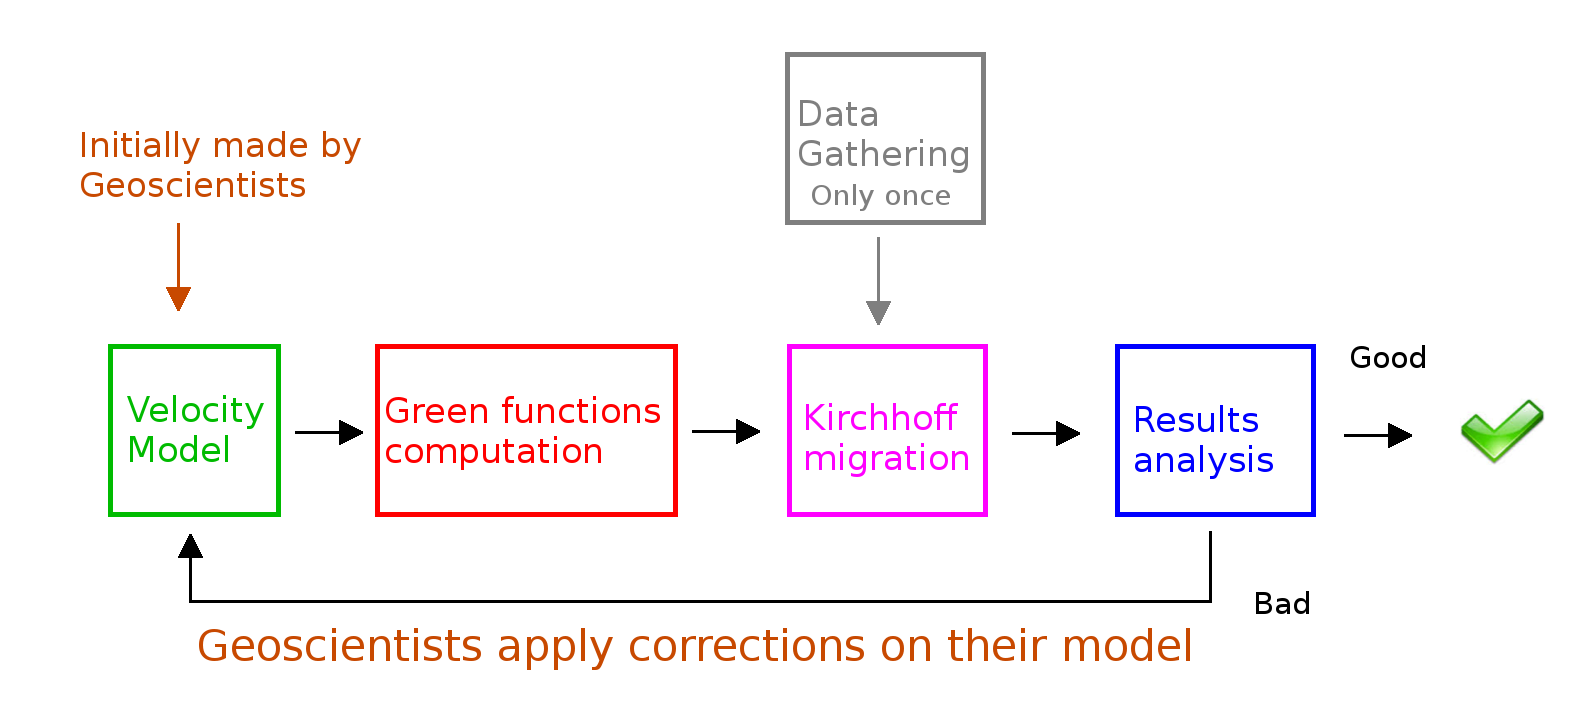
\includegraphics[scale=0.25]{kirchhoff-process}
	\caption{Building process of a seismic velocity model \label{fig:kirchhoff-process}}
\end{figure}

\subsection{Velocity model}
The velocity model describe the propagation speed of the waves into the different layer of the underground.
Geophysicists create a model and want to verify its correctness.
Their goal is to find the best model that explain the data.
They use the Kirchhoff migration that determine where are the limits between layers.
This method processes data called traces.
They are the output from a seismogram (receiver) at the surface after the emission (source) of a wave into the ground.
If the model is coherent with the image generated by the migration, the model is correct.
Otherwise, the model is adjusted by geophysicists and the migration is re-used to obtain a new image.
This process is repeated until the image and the model are coherent.

\subsection{Data gathering}
Data are produced during an acquisition campaign.
A campaign contains several shots.
A shot is a seismic impulsion launched through the ground.
It is the source (see Figure \ref{fig:shot}).
There is several receiver.
They are seismograms placed on a 2D grid on the ground (see Figure \ref{fig:source-receiver}).
The source is moved on the 2D grid and produces shots.
So a trace is the result for a given shot (source) and a given seismogram (receiver).

\begin{figure}[H]
	\centering
	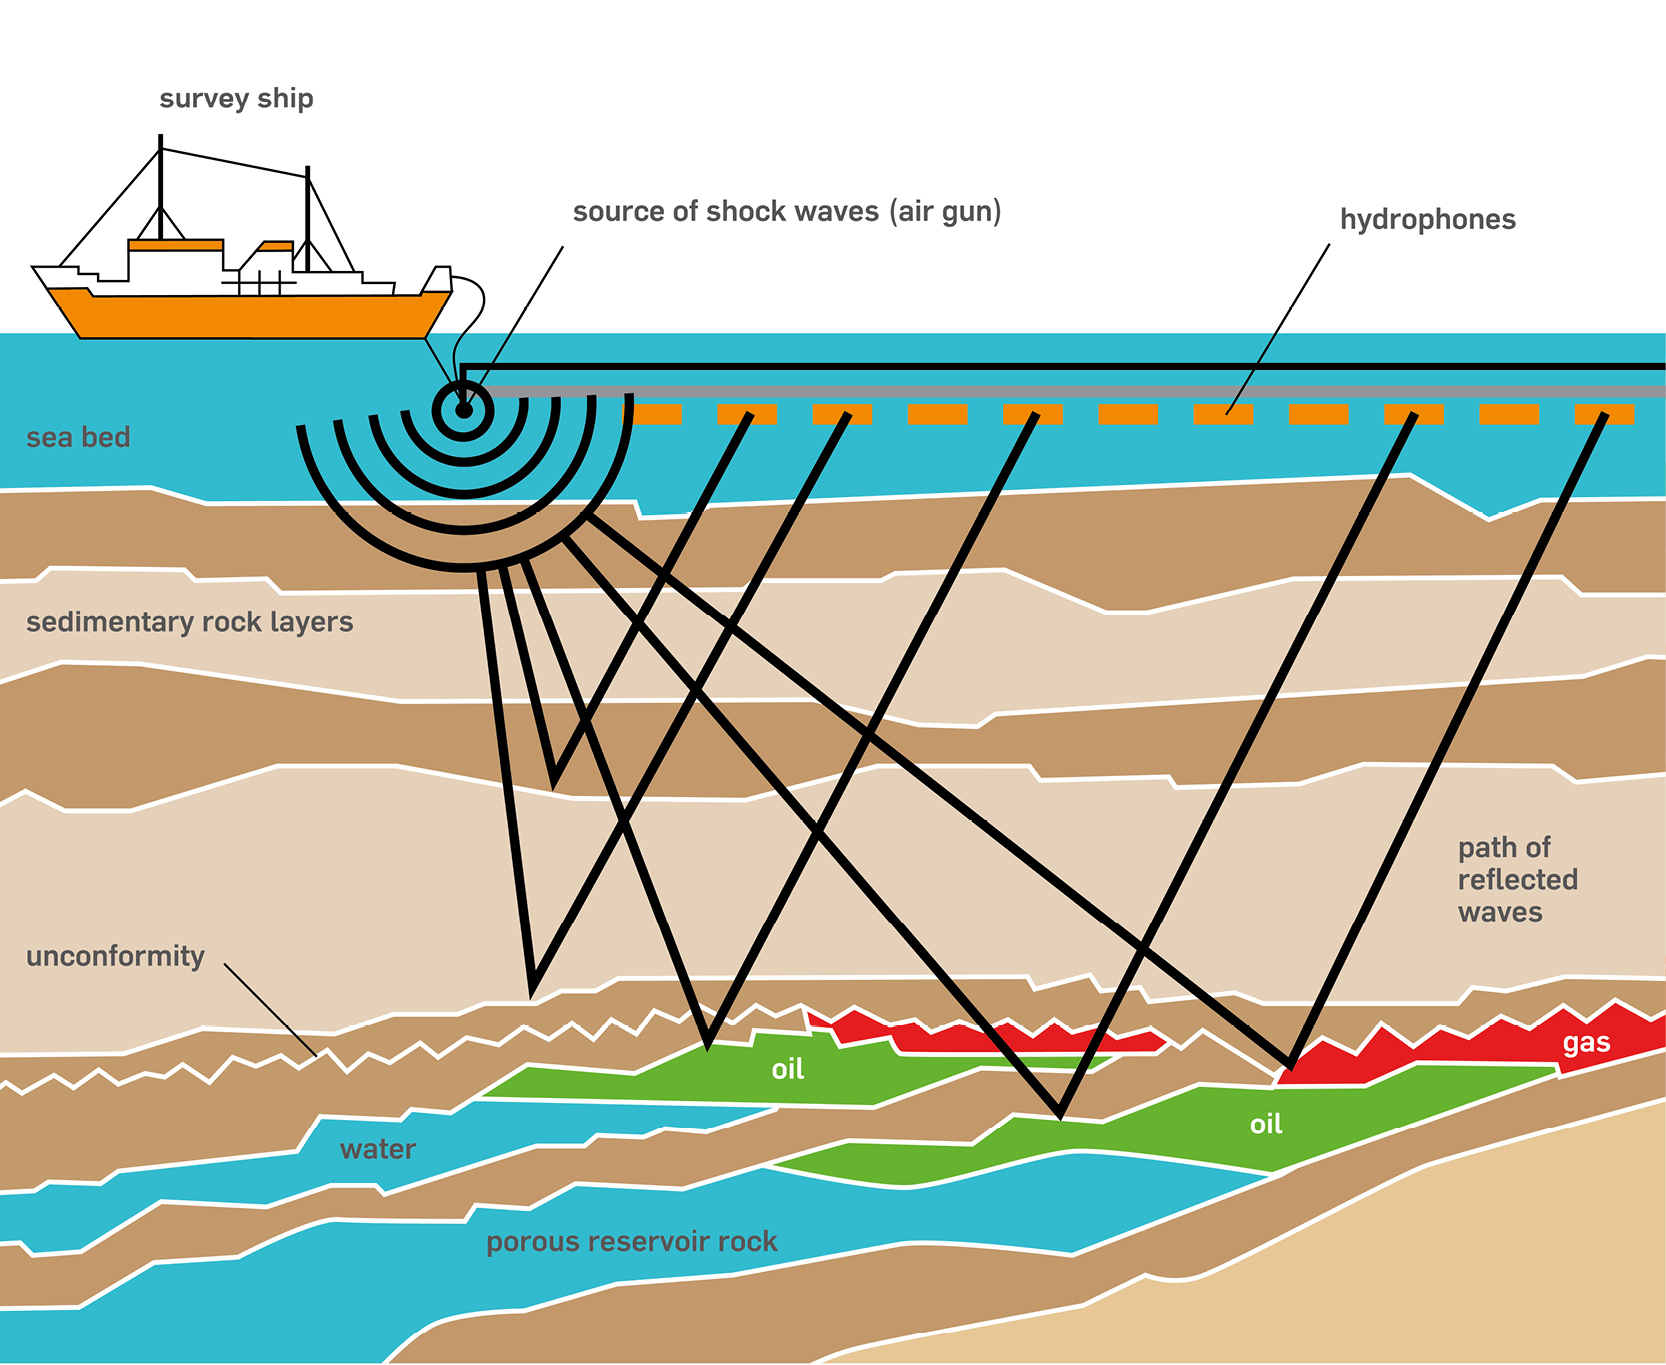
\includegraphics[scale=0.75]{oss}
	\caption{Shot during Data acquisition \label{fig:shot}}
\end{figure}
\begin{figure}[H]
	\centering
	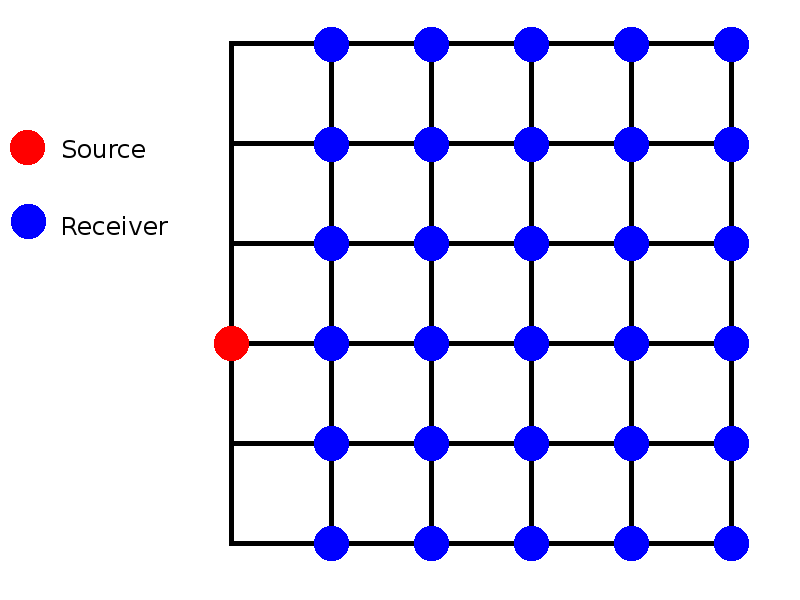
\includegraphics[scale=0.37]{gridSR}
	\caption{Shot and seismograms \label{fig:source-receiver}}
\end{figure}

The acquisition campaign gives a huge amount of traces since there is a lot of receiver and several shots.
A trace contains the coordinates of the source and the receiver and the data from the seismogram.

\subsection{Green functions}
The Green functions represent the response and the behaviour of the wave when the source is a Dirac impulse.
They allow to solve the wave equation using an integral formula in function of the source of the wave.
The behaviour of the wave in the ground depends on the velocity model.
Usually, Green functions are pre-calculated and stored on disk for a 2D grid on surface and a 3D grid underground.
During the building of the model and the migration, Green functions are retrieved from disk.

In the Kirchhoff migration, the Green functions are used to estimate the travel time between 2 points depending on the velocity model.
We estimate the travel time between a source S and a point P of the image ($T_{SP}$) then between P and a receiver R ($T_{PR}$).
So we can deduce $T_{SPR} = T_{SP} + T_{PR}$ (see Figure \ref{fig:Green_functions1}).

\begin{figure}[H]
	\centering
	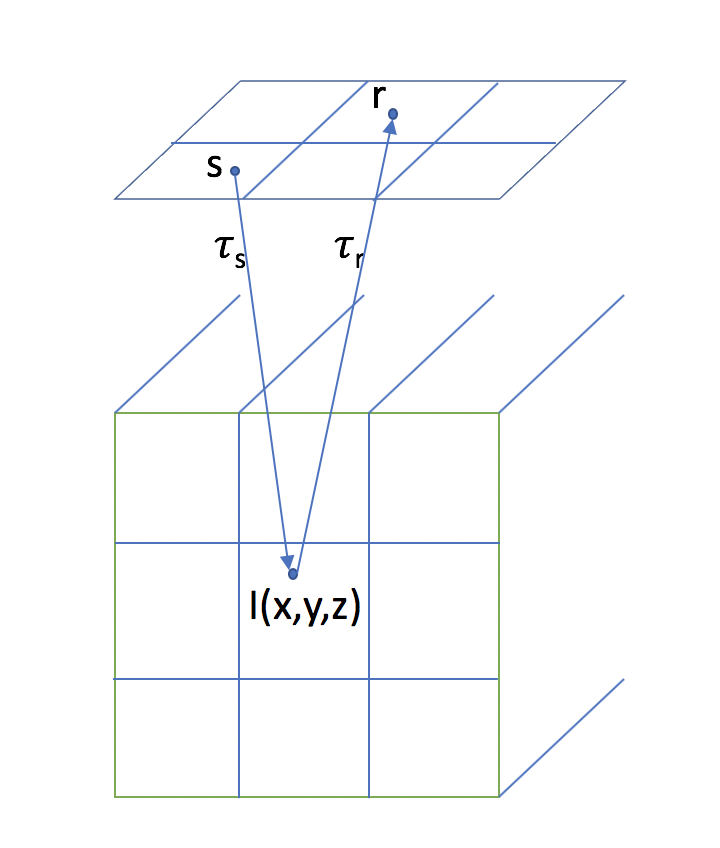
\includegraphics[scale=0.6]{img1}
	\caption{Wave travel between S and R through P\label{fig:Green_functions1} from \cite{rapport_Total_Petiton}}
\end{figure}

Green functions are pre-calculated for a 2D grid at the surface and for à 3D grid underground (see Figure \ref{fig:grids}).
Moreover, a block of the 3D grid contains an image at a finer grain.
Therefore, it is necessary to interpolate or extrapolate the Green functions for the points into the finer grid (see Figure \ref{fig:fine_coarse_grid}).

\begin{figure}[H]
	\centering
	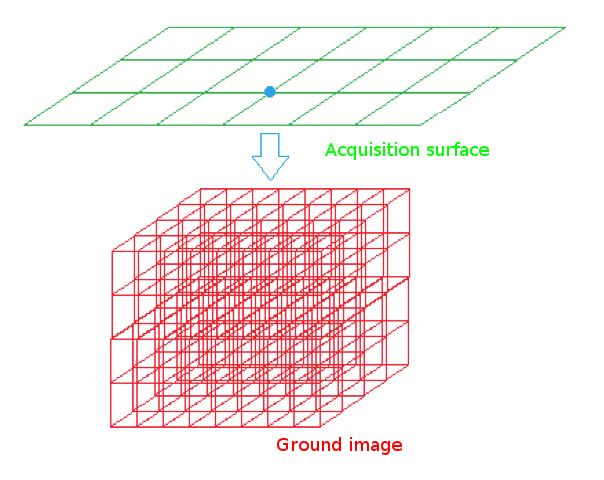
\includegraphics[width=.55\textwidth]{figure8rapportP2}
	\caption{2D and 3D grids \label{fig:grids} from \cite{rapport_Total_Petiton}}
\end{figure}

\begin{figure}[H]
	\centering
	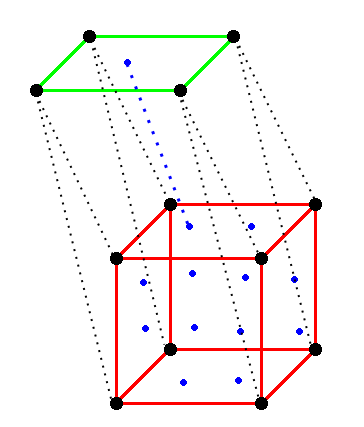
\includegraphics[width=.55\textwidth]{fctGreenInterpolation}
	\caption{Coarse grid and points from the finer grid \label{fig:fine_coarse_grid}}
\end{figure}

\subsection{Kirchhoff migration \label{sec:kirchhoff}}
The Kirchhoff migration produces a 3D image of the subsurface by retrieving the position of the reflection points in order to show the different layers of the ground.
To do so, find the time a wave need to travel from a source to a point $(x,y,z)$ in the image and travel back from this point to the receiver is necessary.
The Green functions in the fine grid give this time.
Then, the trace\footnote{http://www.iris.washington.edu/ds/nodes/dmc/manuals/irisfetchm/} (Figure \ref{fig:kir_trace}) has a peak when the wave arrives to the receiver.
This corresponds to the time it needs for the trace to travel from the source to the receiver into the ground.
For a given source and receiver, if the time a wave need to travel trough the point $(x,y,z)$ and the time to the peak of the trace match then $(x,y,z)$ can be a candidate to a reflection point.

\begin{figure}[H]
	\centering
	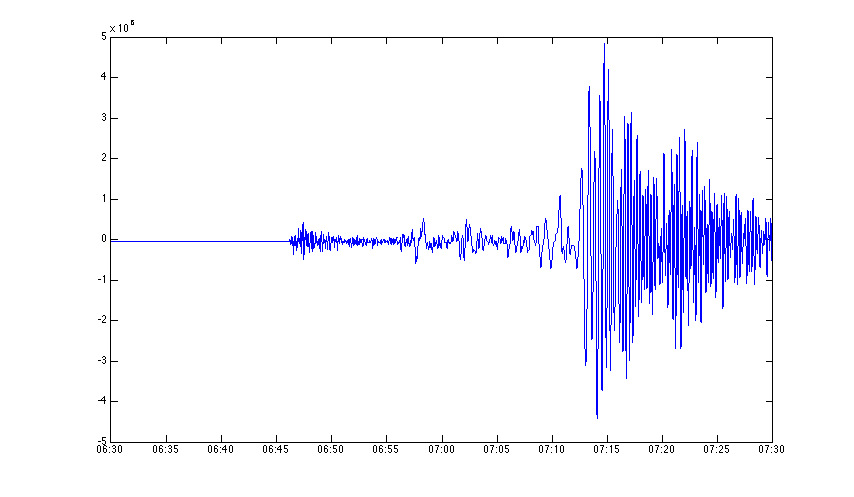
\includegraphics[width=.75\textwidth]{trace}
	%http://www.iris.washington.edu/ds/newsletter/vol14/no1/7/direct-data-access-from-within-matlab/
	\caption{A trace from the IRIS-DMC repository\label{fig:kir_trace}}
\end{figure}

Moreover, we know the Green functions for a coarse grain of the image, so it is possible to know if the points in the sub-domain of the coarse grid will match the time from the trace.
If the time matches, the points will be studied at a finer grain.
Otherwise, the points of the part of the coarse grid will not be candidates to a reflection point and those points will be ignored for the selected trace.

At the finer grain level, when the block of coarse grid matches with the time of the trace, the Green functions are interpolated or extrapolated for each point in the block.
This give the travel time $T(x,y,z)$ between the source and the receiver passing by the point $(x,y,z)$.
Then, only the points matching the time of the trace are kept.
Those points are likely true reflection points.
An arbitrary value (the aperture) $A_{s,r}(x,y,z)$  \cite{XHCCC2014} that favours points with less awkward reflection angles, and positions that are more likely to match the true reflection point, can be calculated.
This value depends on the coordinates of the receiver 'r', the coordinates of the source 's' and the point $(x,y,z)$.
The value $A_{s,r}(x,y,z) t_{s,r}(x,y,z)$ expresses the intensity of the contribution of the trace for the point $(x,y,z)$.

The image at a point is generated by summing the contribution of all the traces that can be a true reflection point :


\begin{equation}
	I(x,y,z)=\sum_{t_{s,r} \in T}A_{s,r}(x,y,z)t_{s,r}(\tau_s(x,y,z) + \tau_r(x,y,z))
\end{equation}

$I(x,y,z)$ is the point $(x,y,z)$ of the image.
$t_{s,r}$ is the trace which has $s$ as source and $r$ as receiver.
$T$ is the ensemble of traces.
$A_{s,r}$ is the amplitude associated to $s$ and $r$.
$\tau_j(x,y,z)$  is the time need for a wave to travel from $j$ (a source or a receiver) to $(x,y,z)$.


In the existing application, the Green functions (the time needed by the sound wave to go from the source or the receiver to the point inside the grid, the values of $\tau$) are pre-computed from the velocity model which is evaluated and imported from the file system when the application is using them.

Moreover, two granularities of grids are used.
The values of $A$ and $\tau$ are computed for the coarse grid and they are interpolated from the computed values for the fine grid.


\subsection{Analysis of the results}
The resulting image is analysed by geophysicists.
If they think that the velocity model is coherent with the image, the model can be exploited.
Otherwise, the velocity model is modified and the process of the Kirchhoff migration is reused until the geophysicists judge that the velocity model corresponds to the data.
	\chapter{Languages}
\label{chap:languages}
\graphicspath{{chapters/languages/}}


\lstdefinestyle{customcode}{
	frame=single,
	numbers=left,
	xleftmargin=2em,
	framexleftmargin=1.8em,
	numberstyle=\color{gray},
%	basicstyle=\small,
}

In Chapter \ref{chap:hpc}, we introduced most of the current task based programming models.
In this chapter, we select a few of them in order to use them in our experiments and implement parallel and distributed applications based on the methods presented in Chapter \ref{chap:methods}.
In this chapter, we study several programming models in three classes of programming models in greater details.
The first class is task based programming models in which tasks are fine grain and running inside only one thread or process.
The second one contains task based programming models that use parallel and distributed tasks that run on multiple processes.
The last class is message passing libraries that are the current commonly used programming model to implement parallel and distributed applications.

\section{Message Passing Interface}
The Message Passing Interface (MPI) \cite{MPIForum} is a standardized norm designed to work on a wide variety of parallel computers.
It defines the syntax of the core library routines to write message-passing applications.
The application uses several processes to make computation at the same time on different cores and uses MPI to send data from one process to another one.
MPI has several implementations (OpenMPI, MPICH2, IntelMPI, \dots) which consist of a set of routines that can be called from C, C++ and Fortran.

The MPI library interface includes point-to-point send/receive operations, aggregate functions involving communication between all processes, synchronous nodes (barrier operations), one-way communication, dynamic process management and I/O operations.
MPI provides synchronous and asynchronous routines as well as blocking and non-blocking operations.
Collective routines involve communications between all processes in a group, for instance MPI\_Bcast (broadcast that sends an array to all of the other processes).

MPI can be used with shared memory programming models like OpenMP or with libraries to send data and make computations on CPUs like CUDA.


\section{Task Based Programming Models}
\subsection{PaRSEC}
PaRSEC \cite{BBDHL2011} \cite{BBDFH2013} (Parallel Runtime Scheduling and Execution Controller) is an engine for scheduling tasks on distributed hybrid environments.

It offers a flexible API to develop domain specific languages.
It aims to shift the focus of developers from repetitive architectural details toward meaningful algorithmic improvements.
Two domain specific languages are supported by Parsec, the Parameterized Task Graph \cite{DBBHD2014} (PTG) and Dynamic Task Discovery \cite{HoHBD2017} (DTD)

In PTG \cite{DBBHD2014}, users would use a parameterized expression of task dependencies combined with PaRSEC which would implicitly infer the communication between nodes and the accelerators.
The users has to provide a description of the data flow of their application and the tasks which are applied on the data.
They also has to provide the tasks that are the source of the data and the tasks that are the destination.
So, this is a compressed algebraic representation of the task graph.
Then, it is transformed into C code using a pre-compiler.
Users need to understand and provide all the data flow of their algorithm to use this model.


DTD \cite{HoHBD2017} is a task-based programming paradigm which provides an alternative way to express task dependency in PaRSEC that achieves a similar purpose to PTG.
Contrary to PTG where users had to express tasks in a parameterized manner, DTD allows them to write sequential constructs (ifs, loops, etc\dots) to insert tasks in PaRSEC.
The tasks are given to the runtime with the data they will use and their mode of usage.
Then, the runtime will compute dependencies out of data pointers used by the tasks.
In a distributed system, the data movements among the nodes are completely implicit.


\lstinputlisting[style=customcode,language=C,
caption=Task in PaRSEC\label{lst:parsec_task}]{chapters/languages/parsec_task.c}

\subsubsection{PaRSEC Task definition}
Listing \ref{lst:parsec_task} shows how to define a task in PaRSEC.
Line 1 defines the name of the task and the integer parameters in input.
This task is called \textit{PMM}.
Line 3 and 4 give the range of those parameters.
In line 6, \textit{dcA} is a data descriptor and is used to align the task on the resources from the descriptor.
Line 8 to 11 describe the dependencies of the task.
Line 13 to 19 are the body of the task.
They contain the computations on the data.
This task calls the \textit{pmm\_core} to process the data stored in the \textit{Ap} and \textit{Bp} pointers.


\subsubsection{PaRSEC Dependency definition}
Line 8 to 11 from Listing \ref{lst:parsec_task} shows how to describe the dependencies of a task in PaRSEC.
The \textit{PMM} task uses two pieces of data \textit{A} and \textit{Inv}.
They are temporary pointers that hold the data that will be used in the task.

\textit{A} is in read-write mode (RW).
It means \textit{PMM} expects a pointer in input that will be called A in the body of the task.
That pointer can be modified and will be transfered into another task.
The data in \textit{A} come from the part $(i,k)$ in the data descriptor \textit{dcA} when $k=0$ and from the data referenced as \textit{$A_{ij}$} in the task \textit{PMM\_D}.
When the task is finished, the data in \textit{A} will be sent as input of \textit{$A_{ik}$} from the task \textit{PMM\_D}.
Indeed, Listing \ref{lst:parsec_pmmd_dep} shows the corresponding dependencies definition.
We find \textit{A} from \textit{PMM} as input for \textit{$A_{ik}$} from \textit{PMM\_D} and \textit{$A_{ij}$} as input for \textit{A} from \textit{PMM}.

\textit{Inv} is in read mode (READ).
It only uses the piece of data named \textit{Inv} from the \textit{Inv} task.

There is also a write mode (WRITE) that output a new piece of data.

Control dependencies can also be added through the \textit{CTL} keyword.
It allows the user to create control flow data which can tell the runtime if a task has to be done before another one.

\lstinputlisting[style=customcode,language=C,
caption=Expression of PMM\_D dependencies\label{lst:parsec_pmmd_dep}]{chapters/languages/parsec_pmmd_dep.c}

This way of expressing the dependencies is error-prone.
Indeed, the user can easily be lost in the definition of the dependencies since he has to replicate them in two tasks (for instance, the input of a task is the output from another one).
Moreover, it can become very complicated when there is a lot of different tasks and condition on the parameters.

\subsubsection{PaRSEC Data definition}
\textit{dcA} is a \textit{two\_dim\_block\_cyclic\_t*}.
This is a matrix data type provided by PaRSEC.
It helps to store two dimensional arrays of matrices in memory.
We use it to store sub-matrices in our block-based LU factorization.
It extends the initial data type \textit{parsec\_ddesc\_t} as for each data type used by PaRSEC.
Listing \ref{lst:parsec_custom_datatype} shows how to extend \textit{parsec\_ddesc\_t} to create a data type called \textit{my\_datatype\_t}.

This data distribution descriptor stores only one data block per MPI \cite{MPIForum} process in the field \textit{ptr}, of size \textit{size} bytes.
However, the user's memory is not manipulated directly by PaRSEC.
It uses \textit{parsec\_data\_t*} as well as \textit{parsec\_data\_copy\_t*}.
\textit{parsec\_data\_t} is an abstract representation of user data.
\textit{parsec\_ddesc\_t} class instantiates at most one per MPI process per user data element.
\textit{parsec\_data\_copy\_t} is a representation of a copy of the user data and multiple instances can exist at the same time.
Distributed Data Descriptors usually manipulate parsec\_data\_t objects, and provide parsec\_data\_copy\_t objects, using PaRSEC functions to instantiate them.


\lstinputlisting[style=customcode,language=C,
caption=PaRSEC custom datatype definition\label{lst:parsec_custom_datatype}]{chapters/languages/parsec_custom_datatype.c}

PaRSEC uses all fields from the \textit{parsec\_ddesc\_t} object.
The user has to fill them in order to implement a new data type.
\textit{myrank} is the rank of the local MPI process.
\textit{nodes} is the number of nodes in the MPI Communicator.
Then, the other obligatory fields are function pointers.
\textit{rank\_of} and \textit{rank\_of\_key} return the rank of a given data element, based on its multidimensional index or its flat key.
\textit{vpid\_of} and \textit{vpid\_of\_key} return the identifier of the Virtual Process that "owns" a data identified by its multidimensional index or its flat key.
\textit{data\_of} and \textit{data\_of\_key} return the parsec\_data\_t* associated with the user data at this multidimensional index position, or for this flat key.

Line 3 to 9 in Listing \ref{lst:parsec_launch} shows how to initialize \textit{dcA} with a built-in function dedicated to that and then how to allocated the memory in each MPI process with \textit{parsec\_data\_allocate} function.

With the definition of these functions, PaRSEC is able to manage efficiently the data from the user.


\subsubsection{PaRSEC Graph execution}
PaRSEC compiler generates code to launch the tasks.
In this case, it is the \textit{parsec\_lu\_new} function as shown in Listing \ref{lst:parsec_launch}.
It takes \textit{dcA} the data descriptor and \textit{bm} which is the number of tiles in each dimension as parameter.
The preprocessor finds them in the source file and put them as input parameters of the function to launch the tasks.

\lstinputlisting[style=customcode,language=C,
caption=PaRSEC tasks launching\label{lst:parsec_launch}]{chapters/languages/parsec_launch.c}


\subsubsection{PaRSEC Granularity}
PaRSEC assigns computation threads to the cores, overlaps communications and computations.
Each task is run into a thread.
Furthermore, PaRSEC tasks are fine grain.

\subsubsection{PaRSEC Tasks re-usability}
Tasks cannot be reused as they are since their dependencies, parameter ranges and alignment are stored in the task definition.
They have to be rewritten for each new application.
However, core computations can be stored into a routine which can be reused into other tasks.

\subsubsection{PaRSEC Scheduling}
The design of the PARSEC runtime system focuses on scalability.
PaRSEC tries to limit task knowledge to processes that are responsible for their execution.
The scheduling decisions are entirely distributed.
Algorithmic correctness should not require control synchronization, and synchronous collective synchronization should be avoided.


\subsubsection{PaRSEC Type of graph}
PaRSEC is mainly based on the expression of data flow dependencies but the user can also give additional control flow dependencies if needed.

\subsubsection{PaRSEC GPU support}
In PTG, the tasks are implemented for CPU by default.
However, PaRSEC is able to move data to the GPU and to call tasks on it.
The code to run on GPU is specified in the \textit{BODY} as for a CPU task and adding the option \textit{[type=CUDA]} to
after the keyword \textit{BODY}.
A function which operates on the data on the GPU can be called in the body of the task.


\subsection{Legion}
Legion \cite{BaTSA2012} is a data-centric parallel programming model.
It aims to make the programming system aware of the structure of the data in the program.
Legion provides explicit declaration of data properties (organization, partitioning, privileges, and coherence) and their implementation via the logical regions.
They are the fundamental abstraction used to describe data in Legion applications.
Logical regions can be partitioned into sub-regions and data structures can be encoded in logical regions to express locality describing data independence.

A Legion program executes as a tree of tasks spawning sub-tasks recursively.
Each tasks specifies the logical region they will access.
With the understanding of the data and their use, Legion can extract parallelism and find the data movement related to the specified data properties.
Legion also provides a mapping interface to control the mapping of the tasks and the data on the processors during the execution of the application.

Legion installation is a bit different than other libraries.
It is not installed as a compiled library.
The user has to compile it each time he compiles an application.
A static library is generated while executing the Makefile provided to compile an application and is included in the executable.
Therefore, compiling an application is taking some time.

\lstinputlisting[style=customcode,language=C,
caption=Legion task\label{lst:legion_task}]{chapters/languages/legion_task.c}

\subsubsection{Legion Task definition}
Legion tasks are implemented as a tree of tasks.
The main function calls Legion runtime to register the top level task which will spawn other tasks.
Those task will also spawn other tasks.
Line 36 from Listing \ref{lst:legion_task} shows how to call Legion runtime to launch the tasks.
Tasks have to be registered into Legion using a \textit{Registrar}.
Line 31 to 34 shows how to do that and bind the task to use CPUs.

Legion tasks need to have generic parameters so that the runtime can call them and pass the data and pieces of information they need.
Line 1 to 3 shows the prototype of a function which is used as a task in Legion.
This task expect two regions which store data that will be accessed in this task and a integer as argument since the task asserts that the size of the region is two (line 4 and 5) and that the length of the arguments is of the size of an integer (line 8).

Data regions are accessed through \textit{FieldId} and \textit{FieldAccessor}.
Line 12 and 15 shows how to get accessors to a region in read mode.
It can be used with an \textit{Iterator} on an index space (as defined on line 18).
This iterator is used as index to the accessors so that pieces of data can be retrieved or set as shown on line 24.


\lstinputlisting[style=customcode,language=C,
caption=Legion data\label{lst:legion_data}]{chapters/languages/legion_data.c}

\subsubsection{Legion Dependency definition}
Dependencies are implicitly defined with the access mode of the regions and the tree of tasks.
Indeed, a task can launch another tasks when it is finished.

\subsubsection{Legion Data definition}
Data are defined through regions of any given type.
To define a region and divide it in sub-regions then run tasks on the sub-regions, an index space and a field space for the region have to be defined.
The index space keeps the coordinates of the values in the multi-dimensional array represented by a region (line 8 from Listing \ref{lst:legion_data}).
The field space defines which type of data there will be in the region (line 9 to 15 from Listing \ref{lst:legion_data}).
It is represented by a number of byte for each coordinate of the field space.
Furthermore, they can be combined into a \textit{LogicalRegion}  (line 16 from Listing \ref{lst:legion_data}).
It will allocate the region of the designed type in memory.
Custom mappers can be used to optimize the data allocation.

This \textit{LogicalRegion} is split into two partitions; a regular block partition and a partition with ghost borders (duplicated values between neighbor sub-regions).
It is done by defining another index space which will record the coordinates of the sub-regions (line 19 from Listing \ref{lst:legion_data}).
Then, the index partitions can be created from the data index space and the sub-regions index space (line 21 to 29 from Listing \ref{lst:legion_data}).
Finally, the \textit{LogicalPartition} which contains the split data can be created from the initial \textit{LogicalRegion} and the newly defined sub-regions index partitions (line 31 to 34 from Listing \ref{lst:legion_data}).


\subsubsection{Legion Graph execution}
The tasks are registered into the runtime system then the user can use the runtime to start executing the tasks from the tree of tasks.

\lstinputlisting[style=customcode,language=C,
caption=Legion launch task\label{lst:legion_task_launch}]{chapters/languages/legion_task_launch.c}

There is several way of launching tasks in Legion.
Tasks can be launched on a \textit{LogicalRegion} and  the task will process all the data of the region.
They can also be launched on all the sub-regions of a \textit{LogicalPartition} at the same time then the scheduler manage the resources on which launch the tasks.
Listing \ref{lst:legion_task_launch} shows how to process sub-regions in this way.
An \textit{IndexLauncher} need to be created to do so.
It needs the identifier of the task which is defined when registering the task, the sub-regions index space on which launch the tasks and arguments for the tasks.
The \textit{LogicalPartition} have to be given to the index launcher so that the tasks can access the data.
This is performed by using the \textit{add\_region\_requirement} and the \textit{add\_field} methods.
These parameters are passed to the task via the runtime as we saw in Listing \ref{lst:legion_task}.
Then we can tell the runtime to execute the tasks with the \textit{execute\_index\_space} method (Line 13 in Listing \ref{lst:legion_task_launch}).

\subsubsection{Legion Granularity}
Tasks are run as thread by the runtime so tasks are fine-grain.

\subsubsection{Legion Tasks re-usability}
Tasks can be registered and launched in another application if it provides the regions and parameters expected by the task.

\subsubsection{Legion Scheduling}
Legion uses a software out-of-order processor (SOOP) to schedule tasks.
It dynamically schedules a stream of tasks.
It is constrained by region dependences.
It is also pipelined, distributed, and extracts nested parallelism from subtasks.
Legion uses a \textit{deferred execution model} which separates the issuing of the operations from when operations are executed.
An issued operation waits for other operations on which it is dependent to complete before executing without blocking the scheduler.

\subsubsection{Legion Type of graph}
Legion tasks are defined as a tree of tasks.

\subsubsection{Legion GPU support}
Legion supports data migrations to GPUs.
Data are accessed through Legion data structure.
Tasks are implemented in C++ and can be launched on GPU.
The user has to create tasks (a C++ class) that extends a Legion \textit{Launcher} (for instance, \textit{IndexLauncher}) and to implement a \textit{cpu\_base\_impl} function to run the task on CPU and a \textit{gpu\_base\_impl} to run on GPU.
When the user register the task, he has to specify that the task will run on GPU.

\subsection{Regent}
Regent \cite{SLTBA2015} is a programming model which simplifies Legion.
Regent compiler translates Regent programs into efficient implementations for Legion.
It results in programs that are written with fewer lines of codes and at a higher level.

\subsubsection{Regent Task definition}
A Regent task is similar to a function.
It is defined with the \textit{task} keyword until the keyword \textit{end}.
It has parameters after the name of the task (\textit{pmm\_d} in Listing \ref{lst:regent_task}).
Regent tasks also need \textit{coherence modes} to specify how the data will be accessed.
They can be in \textit{reads}, \textit{writes} or both modes.
On line 4 from Listing \ref{lst:regent_task}, there is an example of read access mode for \textit{B} as well as read and write access mode for \textit{A}.
Line 5 to 12 are the computations in the task.


\lstinputlisting[style=customcode,
caption=Regent task\label{lst:regent_task}]{chapters/languages/regent_task.rg}

\subsubsection{Regent Dependency definition}
Dependencies between tasks are automatically inferred by Regent compiler from input modes.
Line 35 to 43 from Listing \ref{lst:regent_main} show examples on how to call a task in Regent.
This limits the parallelism that can be detected and create additional dependencies when the system is not sure that the tasks are independent.

\lstinputlisting[style=customcode,
caption=Regent application\label{lst:regent_main}]{chapters/languages/regent_main.rg}

\subsubsection{Regent Data definition}
Data types are stored in regions.
The regions can be partitioned and tasks can be executed on subregions.
Custom types can be defined and used as base in regions.
Regions are multi-dimensional arrays.

Line 24 to 27 from Listing \ref{lst:regent_main} define a partitioned region A.
First, the index space of the region itself is created.
Then, the index space of the partition is created.
It is a 2D array of size $nt * nt$ where $nt$ is the number of sub-region in each dimension.
The region \textit{A} can be created out of the index space of the region in line 26.
It creates a 2D region of doubles.
Finally, \textit{A} can be divided in sub-regions.
To do that, the function \textit{make\_partition\_mat} which is defined in line 6 is used.
This function puts each point in \textit{A} into a sub-region.
It is done by using coloration.
Each point is given a color and goes into one of the sub-region.
This function separates the initial region into regular blocks.

The data in an index space are accessed using an \textit{int2d} data structure.
It represents the coordinates of the point.
Each sub-region keeps the index space of the initial region.
Therefore, the lower bound is added to the \textit{int2d} while accessing the values in the task (line 8 in Listing \ref{lst:regent_task}).
\textit{int2d} are also used to access sub-regions as in line 40 of Listing \ref{lst:regent_main}.


\subsubsection{Regent Graph execution}
The tasks are launched through the main function.
Regent compiler converts code into Legion code so the tasks are executed using Legion execution model.
Main function is registered into Regent using \textit{start} function (line 46 from \ref{lst:regent_main}).
It is the starting point of the application.


\subsubsection{Regent Granularity}
Tasks are run as Legion tasks.
They are run into a thread.
Furthermore, they are fine-grain tasks.

\subsubsection{Regent Tasks re-usability}
Tasks can be reused.
They can be stored in another regent file which can be included in another application.
Then, tasks can be called as they are from the other application.

\subsubsection{Regent Scheduling}
Legion scheduling policy is used here.

\subsubsection{Regent Type of graph}
As Regent code is converted in to Legion code, Regent uses Legion tree of tasks that are spawn recursively starting from the main task.

\subsubsection{Regent GPU support}
Regent supports generation of CUDA code for Legion.
A task can be converted to GPU code instead of CPU code by annotating the task with \textit{\_\_demand(\_\_cuda)}.
Regent will then generate CUDA code for Legion that will be executed by Legion runtime.


\subsection{TensorFlow}
TensorFlow \cite{AABBC2016} (\url{https://www.tensorflow.org}) is “open source software library for high performance numerical computation”.
A TensorFlow program consist of a set of Operations arranged into a graph and run by a Session.
The Tensors contain the data and are used by the Operations.
A Tensor is a set of primitive values shaped into a multidimensional array.
An Operation runs computations on the provided Tensors.
TensorFlow deduces the graph from the used Operations.
It provides a lot of built-in Operations in its Low Level API.
It also provides a higher-level API which can be used to implement Machine Learning and AI algorithms.
Most of the algorithms are related to model training and layers of neural networks.
Thus, the high-level API cannot be used to implement non-AI based applications.

The Python package of TensorFlow is easy to install through pip.
For the other languages (C, Java, Go, \dots), binaries can be downloaded and have to be linked in the program.
There is also the possibility to build it from sources.

\lstinputlisting[style=customcode,
caption=TensorFlow block-based LU factorization\label{lst:tf_app}]{chapters/languages/tensorflow_app.py}

\subsubsection{TensorFlow Task definition}
In TensorFlow, Operations are tasks which run on a subset of the problem.
New Operations can be added into TensorFlow.
They have to be implemented in C++ and inserted into the source code of TensorFlow.
The user has to compile it from sources in order to have the new Operations available.
There is several steps to follow : register the Operation, implement the Operation into a kernel, make it compatible with the devices (CPU and GPU) and re-build TensorFlow with the new Operation.


\subsubsection{TensorFlow Dependency definition}
Dependencies between the Operations are computed by TensorFlow system.
They are inferred from the data accessed and the order of the calls.
This limits the parallelism that can be detected and create additional dependencies when the system is not sure that the Operations are independent.

\subsubsection{TensorFlow Data definition}
In TensorFlow, data are managed through Tensors.
It is a multi-dimensional array that store several pieces of data of the same type.
Those data can be integers, doubles, complexes or strings.
Other data structure are not supported.
However, other data structures can be serialized into strings and stores into Tensors as strings.

TensorFlow also provides Variables.
They are used to represent shared and persistent data.
They can be created with Tensors as base.

TensorFlow Python binding offers the possibility to import data from a \textit{numpy} array and create a Tensor out of it.

\subsubsection{TensorFlow Graph execution}
The graph is built on the run when TensorFlow has inferred the dependencies between the Operations.
It is executed through a Session.
The user has to create a Session and use it to run the computation on the different Tensors to launch the Operations and obtain the output of the computations.

Listing \ref{lst:tf_app} shows on line 8 how to create a Session.
It also show on line 15 and 16 how to initialize Variables through the Session.
line 25 to 27 shows how to use the Session to perform the Operations on the Tensors.


\subsubsection{TensorFlow Granularity}
TensorFlow Operations run on a CPU or on a GPU depending on the resources available and the availability of the implementation of the kernel for the type of device targeted.

\subsubsection{TensorFlow Tasks re-usability}
Operations can be reused on different architectures if their implementation is available for this architecture.

\subsubsection{TensorFlow Type of graph}
TensorFlow uses a data flow graph inferred from the Operations on Tensors used in the application.

\subsubsection{TensorFlow GPU support}
TensorFlow is designed to support GPU.
Indeed, TensorFlow Operations can be implemented to run on GPU and/or CPU.





\subsection{HPX}
High Performance ParalleX (HPX) \cite{KHASF2014} \cite{KAHBS2019} is a C++ Standard Library for Concurrency and Parallelism.
It implements the facilities defined by the C++ Standard and functionalities proposed as part of the ongoing C++ standardization process.
It also extends the C++ Standard APIs to the distributed case.
The goal of HPX is to create a high quality, freely available, open source implementation of a new programming model for conventional systems.

HPX API implements the interfaces defined by the C++11/14/17/20 ISO standard and respects the programming guidelines used by the Boost collection of C++ libraries.
It aims to improve the scalability of current applications.
It also tries to expose new levels of parallelism which are necessary to take advantage of the future systems.

HPX is an open-source implementation of the ParalleX execution model.
This model focuses on overcoming the four main barriers to scalability (Starvation, Latencies, Overhead, Waiting for contention resolution).

\lstinputlisting[style=customcode,language=C++,
caption=HPX task \label{lst:hpx_task}]{chapters/languages/hpx_task.cpp}


\subsubsection{HPX Task definition}
In distributed HPX applications, tasks are defined through \textit{HPX\_PLAIN\_ACTION} macro.
Actions can be launch on a local node or a remote node by the scheduler depending on the available resources and the location of the data.
Actions are used to retrieve the data and apply computations on them.
Those data are managed by a data server (\textit{partition\_server} in Listing \ref{lst:hpx_data} which will be discussed later) which is used to keep track of the data and is used by the runtime to move data around.

\textit{partition\_data} is a class used to store data.
It uses a more efficient and specialized implementation than the standard \textit{Vector}.
It stores the data on which tasks run computations.
The \textit{partition\_server} returns futures on calling the \textit{get\_data} function.
The futures are placeholders that are used to ask for data that will be delivered when they are available.
The \textit{dataflow} (on line 19 in Listing \ref{lst:hpx_task}) will wait for the data from the future to be available then execute the function given to it asynchronously (\textit{pmm\_d\_core} on line 22) and pass the data to it.

The \textit{pmm\_d\_core} function will make the actual computations on the data.

\subsubsection{HPX Dependency definition}
Dependencies on tasks are expressed with futures on data used in the tasks and actions.
The actions previously defined helps to wait for the data from the futures to be available.
The actions can now be called with actual data in order to have a complete application.
Listing \ref{lst:hpx_dep} shows an example of using actions to launch tasks on data held by futures.

First, \textit{spaces} (vectors of \textit{partition\_data}) which contains the data are created then initialized (on line 8 to 17 in Listing \ref{lst:hpx_dep}).
\textit{locidx} is an in-lined function that compute the locality on where to put data in a round robin way.
Actions are instantiated so that they can be used.

To launch actions, an \textit{Operation} has to be defined by binding a locality (a position on where the task should be run) and placeholders which will be used to pass data to the action later on.
Finally, the \textit{dataflow} function can be used to launch the action while waiting for the data held by the future.
Line 27 to 30 in Listing \ref{lst:hpx_dep} is an example on how to create the \textit{Operation} and call the \textit{dataflow} function to launch the \textit{inv\_part\_action} which wrap a function that will process the data.

\lstinputlisting[style=customcode,language=C++,
caption=HPX dependencies \label{lst:hpx_dep}]{chapters/languages/hpx_dep.cpp}

\subsubsection{HPX Data definition}
Data are stored into a \textit{partition\_data} structure.
Those are held by futures to wait for their availability and create dependencies between the tasks.
Then the actions make request to the \textit{partition\_server} to get the data in a future and wait for them.
The partition server is implemented and registered to HPX runtime as a component.
It generates code that can be used to get the data and use them on the tasks.
The \textit{get\_data} function is also registered here.
Listing \ref{lst:hpx_data} has the implementation of the \textit{partition\_server}.
It shows the use of HPX macros to register and set up the \textit{partition\_server}.


\lstinputlisting[style=customcode,language=C++,
caption=HPX data \label{lst:hpx_data}]{chapters/languages/hpx_data.cpp}

\subsubsection{HPX Graph execution}
There is several ways to initialize HPX runtime and execute applications.
One of the way is shown in Listing \ref{lst:hpx_launch}.
The main function has to initialize HPX via the function \textit{hpx::init} which takes Boost command line options description which helps to parse command line arguments as input.
HPX runtime launch the \textit{hpx\_main} function which takes Boost command line options as argument so that the user can get command line arguments.

In the \textit{hpx\_main} function, a few parameters are extracted from the Boost command line option map.
Then the \textit{stepper} is instantiated so that the function \textit{do\_lu} which initializes the data, launches the tasks and outputs futures containing the processed data.
Furthermore, the data in the future are waited to make sure that every computation was done and use them later.
They could have been used without waiting for them before hand so that any computation that would depend on the results of \textit{do\_lu} could have been tried before every computation from \textit{do\_lu} are finished in order to maximize the use of the available resources.
Finally, \textit{hpx::finalize} function is called to shutdown HPX runtime at the end of the application.


\lstinputlisting[style=customcode,language=C++,
caption=HPX launch \label{lst:hpx_launch}]{chapters/languages/hpx_launch.cpp}

\subsubsection{HPX Granularity}
The tasks are single threaded functions called on the local node or on a remote node by the runtime.
They are fine-grain tasks.

\subsubsection{HPX Tasks re-usability}
The \textit{stepper} structure can be reused to store tasks and implement another function which will use the tasks as base.
Tasks and actions may be stores in a better environment so that they can be used more easily.

\subsubsection{HPX Scheduling}
HPX scheduler coordinates execution of tasks.
It tries to maximize throughput of the cores, prioritize work according to need and minimize waiting time.
HPX creates \textit{worker} (hardware) thread per core on startup on which it runs its own Task Scheduler.
HPX tasks are executed on the HPX worker (OS) thread.
Each HPX 'task' is referred to as a lightweight thread.

\subsubsection{HPX Type of graph}
The data flow graph is provided by the user through futures and the \textit{dataflow} function.

\subsubsection{HPX GPU support}
HPX provides GPU support through CUDA futures.
They work as the regular futures but allows to execute functions on GPUs.
By default, the user has to use a future to execute CUDA functions to allocate memory on the device with CUDA, copy data to the device, make operations on the data and copy the results to the host.
HPX also provides allocators which helps to manage memory on the device and copy data between the host and the device.

\section{Parallel and Distributed Task Based Programming Models}
\subsection{YML+XMP}
% TODO Mention Docker

\subsubsection{YML}
YML \cite{DelaP2004} \cite{DelEP2006} is a development and execution environment started in 2000 for scientific workflow applications over various platforms, such as HPC, Cloud, P2P and Grid.
YML defines an abstraction over the different middlewares, so the user can develop an application that can be executed on different middlewares without making changes related to the middleware used.
YML can be adapted to different middlewares by changing its back-end (Figure \ref{fig:schema}).
Currently, the proposed back-end \cite{TsSHP2013} uses OmniRPC-MPI \cite{SaHTS2001} \cite{SatBT2003}, a grid RPC which supports master-worker parallel programs based on multi SPMD programming paradigm.
This back-end is developed for large scale clusters such as Japanese K-Computer and Poincar\'e, the cluster of the \textit{Maison de la Simulation}.
A back-end for peer to peer networks is also available.
Moreover, YML also supports fault tolerance \cite{TsuPS2015}.
The Figure \ref{fig:schema} shows the internal structure of YML.

\textbf{YML applications} are based on a graph and a component model.
They represent the front-end.
YML defines components as tasks represented by nodes of a graph which is expressed using the YvetteML language.
It expresses the parallelism and the dependencies between components.
The application is a workflow of components execution.
Components can be called several times into one application.
The graph can be seen as the global algorithm of the application and the components as the core code.

\begin{figure}[h]
	\caption{YML software architecture \label{fig:schema}}
	\medskip
	\centering
	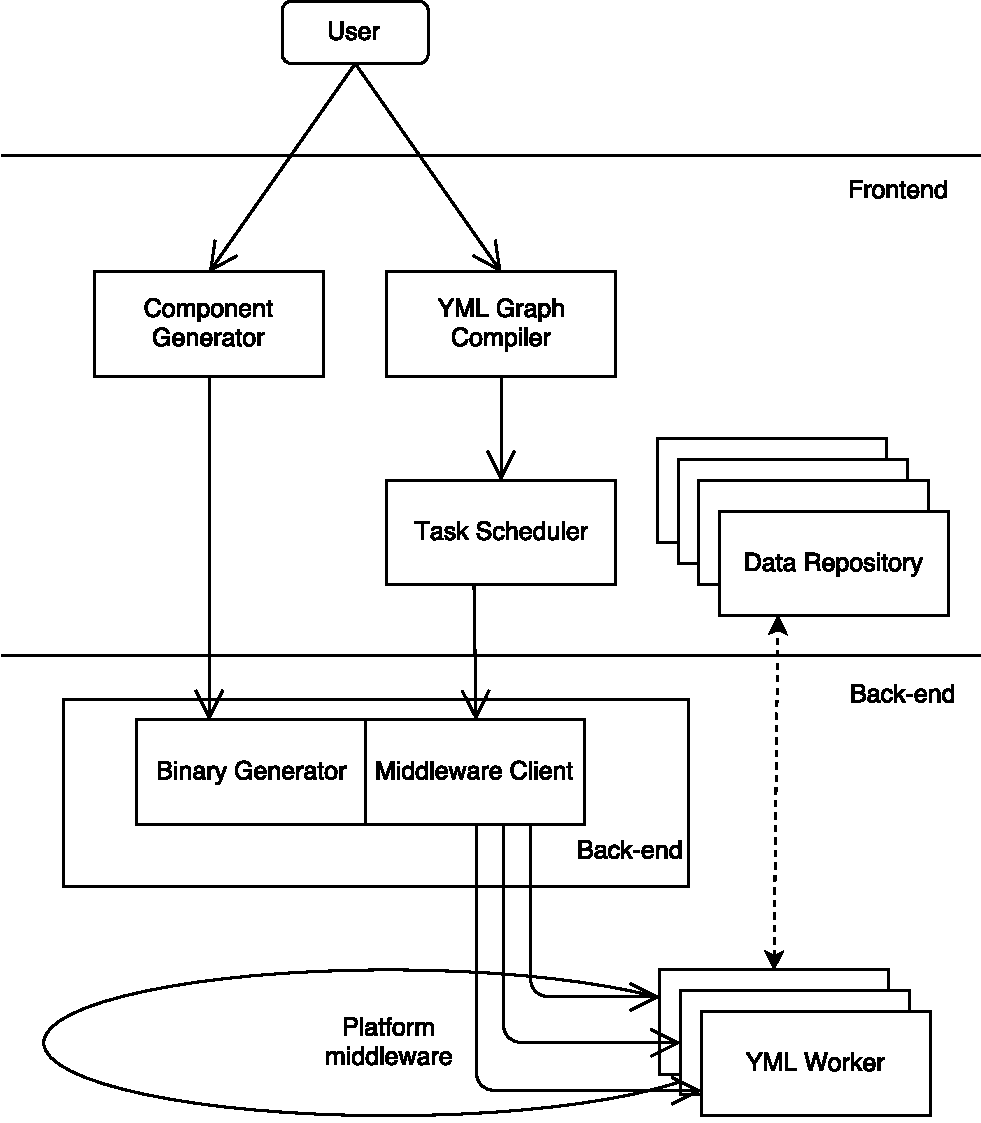
\includegraphics[width=.5\textwidth]{schema.pdf}
\end{figure}

\textbf{The component model} defines three classes of components : Graph, Abstract and Implementation.
They are encapsulated using XML.
They are made to hide the communication aspect and the code related to data serialization and transmission.

\begin{itemize}
	\item Graph components contain the name, a description of the application and the graph written using YvetteML.
	This component also defines global parameters.
	They are data that can be used in components.
	Abstract components are called with the keyword \textit{compute}, their name and the list of parameters they need.
	\item Abstract components contain the name, the type (abstract) and a description of the component.
	They also define the parameters of the data coming from the global application and describe their use in the component (if the data are consumed, modified or created).
	\item Implementation components contain the name, the type (implementation), a description, the name of the abstract component associated, the language used, the external libraries that YML has to deploy and the source code.
	The links of the libraries are installed in YML then they can be used in the implementation component and YML deploys them when needed.
	The source code can also be written in several programming languages, including, for the moment, C/C++, Fortran or XscalableMP (XMP) \cite{XMP}.
\end{itemize}

These categories of component allow re-usability, portability and adaptability.

\textbf{The Component generator} registers the Abstract and Implementation components in YML and the data they need.
The Component generator starts to check if the abstract components exist then it extracts the source code and the information needed to create a standalone application.
The generator also adds the code to import and export the data from the file system.
Afterwards, the Component generator calls the Binary Generator (Figure \ref{fig:schema}) to compile the generated application.
It uses the compiler associated to the language filled in the Implementation component.

\textbf{The Graph compiler} generates the YML application by compiling the Graph component.
It checks that all the components called exist, then verifies that the YvetteML graph is correct.
It also extracts the control graph and the flow graph from the Graph component and the Abstract components.
It creates a binary file containing the application executable with the YML scheduler.

\textbf{The scheduler} manages the computational resources and the data of the application during its execution.
A set of processes is allowed to YML to run the application.
The scheduler explores the graph at runtime (Figure \ref{fig:schema}) to determine which component has to be run.
A component can be run if the execution of the previous components is finished, the data and the computational resources are available.
The scheduler runs the component of the application on a subset of the processes through a worker.
The scheduler sends the component (as shown in the Figure \ref{fig:schema}) to a worker through the middleware.
It executes the component on the subset of processes that manages the worker.
Several workers can run at the same time if there are enough processes available.

Data are stored in a repository created in the current repository at the launch of the application.
The data are read by the components that need them.
The components produce or/and create data and write them in the repository.

\subsubsection{XcalableMP}
XcalableMP (XMP) \cite{XMP} is a directive-based language extension for C and Fortran,  which allows users to develop parallel programs for distributed memory systems easily and to tune the performance by having minimal and simple notations.
XMP supports (1) typical parallelization methods based on the data-/task-parallel paradigm under the "global-view" model and (2) the co-array feature imported from Fortran 2008 for "local-view" programming.

The Omni XMP compiler translates an XMP-C or XMP-Fortran source code into a C or Fortran source code with XMP runtime library calls, which uses MPI and other communication libraries as its communication layer.

Figure \ref{fig:xmpprog} is an example of XMP programming.
A dummy array called {\bf template} indicates data index space and is distributed onto the nodes.
Each element of the array is allocated to the node where corresponding template element is distributed.

\begin{figure}
	\centering
	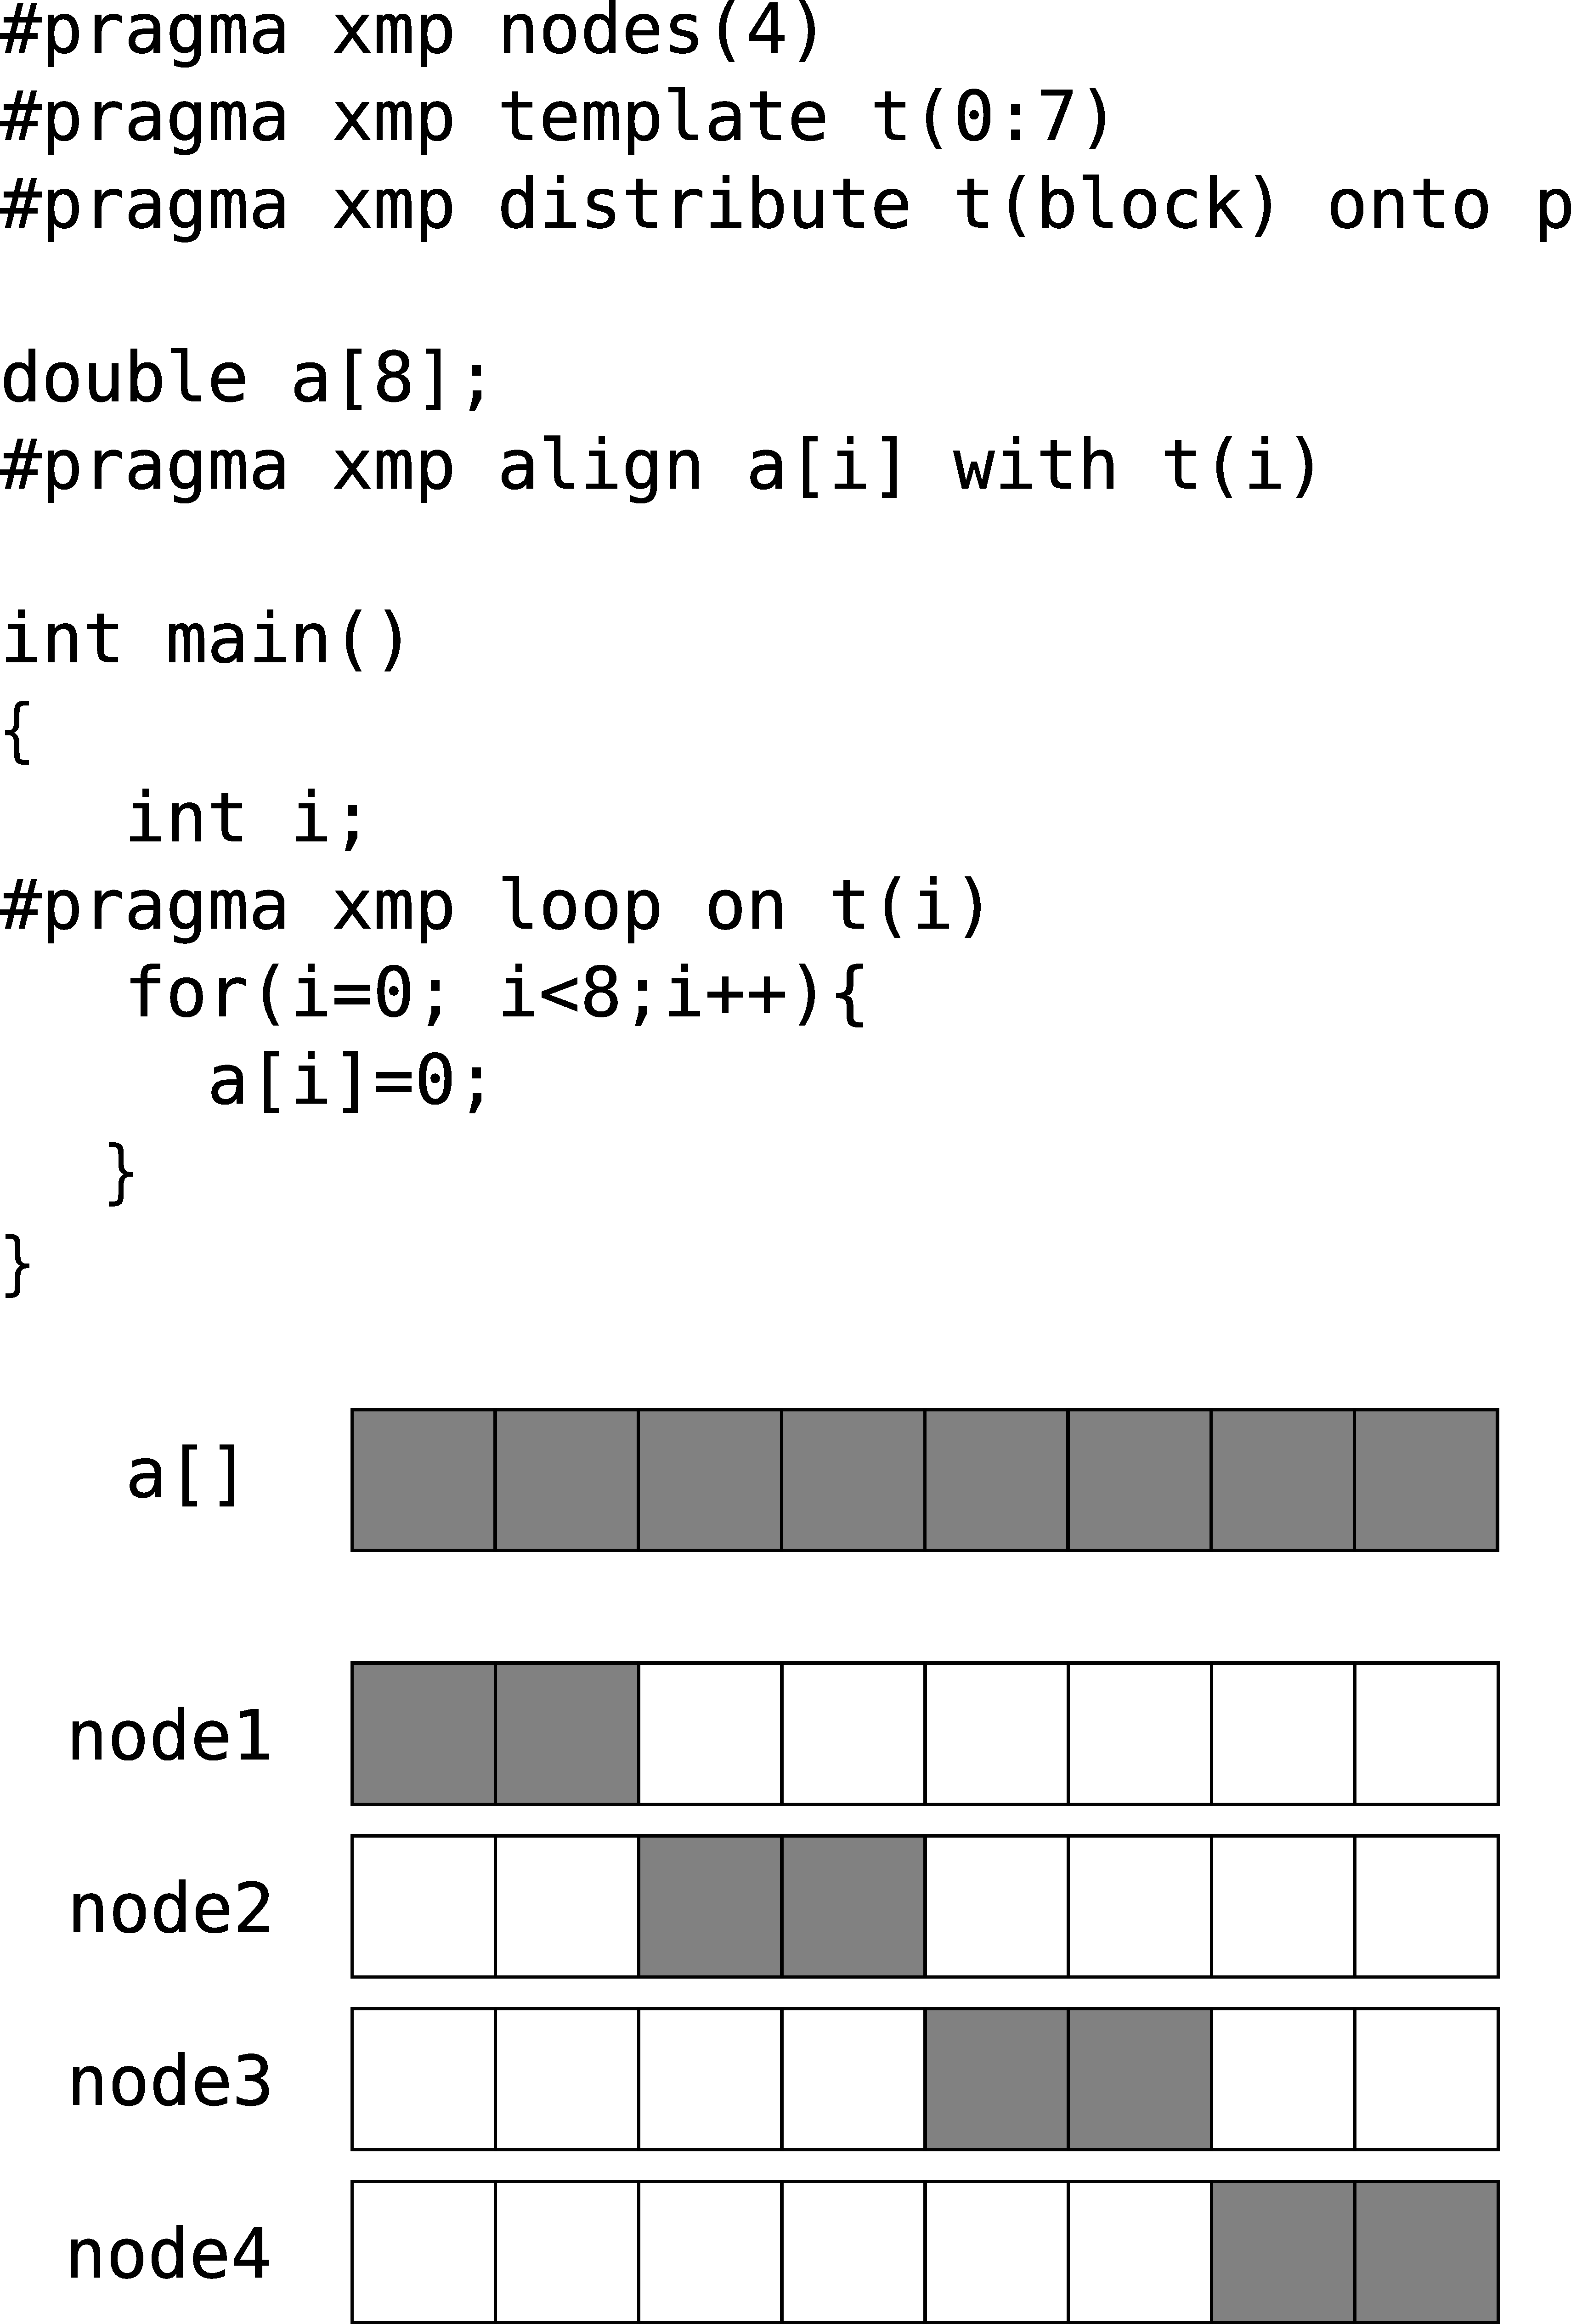
\includegraphics[width=.35\textwidth]{xmp-example.pdf}
	\caption{Example of XMP programming \cite{GuTPS2019}\label{fig:xmpprog}}
\end{figure}

\subsubsection{YML+XMP}
For the experiments, we use XMP to develop the YML components as introduced in \cite{TsSHP2013}.
This allows two levels programming.
The higher level is the graph (YML) and the second level is the PGAS component (XMP).
In the components, YML needs complementary information to manage the computational resources and the data at best : the number of XMP processes for a component and the distribution of the data in the processes (template).
Line 5 to 11 from Listing \ref{lst:yml_task} shows the additional information provided to YML by the user in the implementation component in XMP.
With this information, the scheduler can anticipate the resource allocation and the data movements.
The scheduler creates the processes that the XMP components need to run the component.
Then each process will get the piece of data which will be used in the process from the data repository.

\lstinputlisting[style=customcode,
caption=XMP implementation component for YML\label{lst:yml_task}]{chapters/languages/yml_task.query}

In this approach, there are no global communications along all the processors (like scalar products or reductions) in the application since applications are divided on component calls that use a subset of the computational resources allowed to the application.
The components running at the same time don't communicate with each other and are run independently.
Global communications take time and consume a lot of energy so reducing them and finding other ways to get the same results saves time and is more power efficient.

\lstinputlisting[style=customcode,
caption=Abstract component for YML\label{lst:yml_task_abst}]{chapters/languages/yml_task_abst.query}

\subsubsection{YML+XMP Task definition}
In YML, implementing a task means to create a component.
There is two type of components to implement; an abstract component and an implementation component which will be be implemented with XMP in this case.
Listing \ref{lst:yml_task_abst} shows an example of abstract component.
Line 2 gives the type of component (abstract), the name of the component and a brief description.
This name will be used in the implementation component and to call the task.
Line 4 and 5 define 2 \textit{Matrix} parameters; one is in input and the other one is used in input and output.
The second matrix will be modified by this task.

Listing \ref{lst:yml_task} contains the actual implementation of the component.
Line 2 sets the name of this component and also tells which abstract component it implements.
Line 4 gives the language used to implement this component.
The languages can also be C++ and Fortran as detailed previously.
It uses XMP in this case.
Line 4 also sets how much cores will be used to run the task on.
In this case, we use a 2D array of $32 \times 32$ CPUs.
Line 5 to 11 describe how to distribute the Matrix \textit{A0} and \textit{B0} (defined in the abstract component) on the allocated cores.
It also defines the size of the matrices used ($512 \times 512$).

The code of the task is contained in the \textit{header}, \textit{source} and \textit{footer} tags.
The code inside the \textit{header} tag will be put at the end of the header part of the generated C source file of the component.
The code from \textit{source} tag is put in the main and the code from the \textit{footer} tag will be put at the end of the generated C file.

\subsubsection{YML+XMP Dependency definition}
Dependencies are defined while creating the graph of tasks.
Listing \ref{lst:yml_graph} shows a YML graph with dependencies between the tasks.
Tasks are called with the keyword \textit{compute}, the name of the component provided in the abstract component and the parameters of the task.
They can be called in bulk with loops.
\textit{for} and \textit{par} are the two statements which can be used to repeat statements.
The \textit{for} loop can be used to call task one after the other.
It creates dependencies to wait for the previous task to be finished before launching the next.
The \textit{par} loop launch every task in the loop body at the same time.
A \textit{par} loop is used on lines 10 and 13 in Listing \ref{lst:yml_graph}.
There is also a \textit{par} statement which can be used alongside with \textit{//} to launch several tasks at the same time.

Additional dependencies can be expressed by using YML locking event system.
The \textit{wait} and \textit{notify} keywords are used to manage the events.
\textit{wait} locks the following operations until the event is released by a \textit{notify} on the same event.
For instance, on line 22, the \textit{XMP\_inversion} task depends on the \textit{p[i][i][i]} which is locked by a \textit{wait}.
This event will be released by the \textit{notify} on line 17 when $k = i + 1$ and $j= i + 1$.
It means that the task \textit{compute XMP\_inversion(A[i][i],B[i])} depends on the task \textit{compute XMP\_prodDiff(A[k][i],A[i][j],A[k][j])}.
This event system is used to infer a graph of dependencies.
It is used to schedule the tasks.

\lstinputlisting[style=customcode,
caption=YML Graph\label{lst:yml_graph}]{chapters/languages/yml_graph.query}

\subsubsection{YML+XMP Data definition}
In YML, data types have to be registered so that it is able to manage them.
They are stored in the \textit{DefaultExecutionCatalog/generators} directory in YML configuration files.
Listing \ref{lst:yml_data} shows an example of the functions to implement with the \textit{Matrix} used in the abstract component.
There is three functions to implement.
The first is \textit{$<$type\_name$>$\_MPI\_Type} which return the \textit{\_MPI\_Datatype} used to import and export the data associated to the type in a task.
It can be a custom MPI type.
\textit{$<$type\_name$>$\_import} and \textit{$<$type\_name$>$\_export} are the two other functions to implement.
They are used to import and export the type from the file system.
MPIIO is used to do so in the Matrix type.

\lstinputlisting[style=customcode,
caption=Matrix XMP type\label{lst:yml_data}]{chapters/languages/yml_Matrix.xmptype.h}

\subsubsection{YML+XMP Graph execution}
The graph is executed by launching the \textit{.yapp} application with the \textit{yml\_scheduler}.
This application is produced by \textit{yml\_compiler}.
With XMP back-end, \textit{yml\_scheduler} is launched with \textit{mpirun -n 1 yml\_scheduler my\_app.yapp}.
It will enable YML to launch tasks in the distributed environment.

\subsubsection{YML+XMP Granularity}
With the XMP back-end, tasks are MPI based applications implemented with XMP so they use multi-processes technology.
Each XMP task can run on several nodes of the global number of nodes associated to the application.
These tasks are coarse-grain.

The C back-end provides multi-threaded tasks.
These tasks can be run on one node.

\subsubsection{YML+XMP Tasks re-usability}
Implementation and abstract components can be reused in another application by calling them again with the \textit{compute} keyword.
However, components implemented in XMP have their number of cores used and size of data fixed.
Unfortunately, they cannot be changed dynamically.
It means that the components have to be recompiled each time one of those parameters is changed or that multiple versions if the component with different parameters have to coexist.

\subsubsection{YML+XMP Scheduling}
When a task dependencies are satisfied, the task is put in the execution queue.
The tasks in this queue are executed when the resources are available.
Furthermore, the tasks are launched on the resources they ask in their implementation.

\subsubsection{YML+XMP Type of graph}
The user defines the control flow graph while giving the dependencies between the tasks.
However, the data flow graph can be extracted from the control flow graph and the access mode of the data provided in the abstract component.

\subsubsection{YML+XMP GPU support}
Support for GPUs depends on the backends used.
The XMP backend does not directly support GPUs.
The user has to use an external library to address the use of GPUs.

Moreover, there is a backend that used XMP and StarPU that can address the usage of GPUs.




\subsection{Pegasus}
Pegasus \cite{DSSBG2005} \cite{DVJRC2015} is a Workflow Management System.
It allows the user to express multi-step computational tasks through a directed acyclic graph (DAG), where the nodes are tasks and the edges denote the task dependencies.
The tasks can be everything  from short serial tasks to very large parallel tasks (MPI for example) surrounded by a large number of small, serial tasks used for pre- and post-processing.

Pegasus provides helpers to execute workflow-based applications in different environments like desktops, clusters, grids and clouds.
It automatically maps high-level workflow descriptions onto distributed resources.
It also locates the necessary input data and computational resources needed during the workflow execution.
Pegasus enables scientists to construct workflows in abstract terms.
It can be linked with several middlewares (HTCondor DAGMan \cite{ThaTL2002}, Globus, or Amazon EC2).

Pegasus is fault tolerant.
Indeed, when there is errors, it can retry the tasks, retry the entire workflow, checkpoint its execution, re-map part of the workflow, try alternative data sources and as last resort, provide a list of the remaining tasks.
Storage is cleaned up during the execution of the workflow.
Thus, data-intensive workflows can get enough space to run their tasks on resources with low-capability storage.
Pegasus also keeps track of what has been done, where, which software was used and their parameters.

Pegasus has been used in a number of scientific domains including astronomy, bioinformatics \cite{PRBBF2016}, earthquake science , gravitational wave physics, ocean science, and others.

\subsubsection{Pegasus Task definition}
In Pegasus, tasks are called \textit{Job}.
Listing \ref{lst:pegasus_task} shows how to define and register a \textit{Job} into Pegasus.
DAX Python API is used to generate the XML file that will be treated by Pegasus to launch the jobs on the available resources.
Line 1 defines the graph which will be populated with the jobs.
Then, line 3 to 7 define the Job with its name space, name and version.
The name of the job corresponds to the name of the Executable defined and registered in Listing \ref{lst:pegasus_reg_exe}.
An executable is registered into a graph with the \textit{addExecutable} method.

\lstinputlisting[style=customcode,
caption=Pegasus task\label{lst:pegasus_task}]{chapters/languages/pegasus_task.py}

A job can also pass arguments to the executable with the \textit{addArgument} method.
String and files can be passed as arguments.
A file \textit{c1} is created and will be used as output as stated on line 7.
An already existent file \textit{b1} will be used as input.
The files have registered into the job with the \textit{uses} method so that Pegasus runtime will be able to manage is and move it across the network if needed.
Finally, the job is registered into Pegasus graph by using the \textit{addJob} method from the graph (on line 8 from \ref{lst:pegasus_task}).

A file could be used as input and output however, the \textit{Link.INOUT} property cannot be used.
It does not seem to be implemented.
Therefore, a task cannot modify a file and needs to have an output distinct from the input.
Moreover, each file is considered as an output by default.
They will be transfered back to the user by the runtime, even the temporary files that has to be created due to the impossibility to use a file name as input and output.
The user has to manually set the temporary files as not wanted as output instead of modifying a file.
This decreases the complexity of the runtime since the data files will be unique.

\lstinputlisting[style=customcode,
caption=Register executable in Pegasus\label{lst:pegasus_reg_exe}]{chapters/languages/pegasus_register_exe.py}

\subsubsection{Pegasus Dependency definition}
Dependencies are simple to add into a Pagasus graph with the Python interface.
Indeed, the graph has a method called \textit{addDependency} that takes the dependency as parameter.
A dependency can be declared by providing if the parent and child jobs.
Listing \ref{lst:pegasus_dep} shows an example of such a dependency.

\lstinputlisting[style=customcode,
caption=Dependecy in Pegasus\label{lst:pegasus_dep}]{chapters/languages/pegasus_dep.py}

\subsubsection{Pegasus Data definition}

Pegasus jobs call executables that process files so the user has to use data files that match the format used by the executables to read or write data from file.
The user has to register data files either as intermediary to transfer data from a job to another as described above or registered to the graph which will be used as input and/or output of the jobs performed by the application.
Listing \ref{lst:pegasus_file} shows an example of files registered to the graph.

\lstinputlisting[style=customcode,
caption=File registration in Pegasus\label{lst:pegasus_file}]{chapters/languages/pegasus_file.py}

\subsubsection{Pegasus Graph execution}
Pegasus Python API generates a DAX which can be executed by Pegasus \textit{pegasus-plan} command.
It will submit the jobs to the resources available to the application and manage the input and output data files.

\subsubsection{Pegasus Granularity}
The jobs can be anything between short one threaded application to large scale multi-node applications based on MPI.

\subsubsection{Pegasus Tasks re-usability}
Jobs can be reused in another application if they use the same arguments and files as input otherwise, they will have to be rewritten.


\subsubsection{Pegasus Scheduling}
By default, Pegasus uses HTCondor DAGMan \cite{ThaTL2002} as underline work-flow manager.
Therefore, it uses HTCondor Schedd to schedule the jobs submitted to HTCondor DAGMan.

Pegasus can use  other back-ends as engine.
The scheduling policy will depend on how the engine manage the jobs submitted to it.


\subsubsection{Pegasus Type of graph}
The user only defines dependencies between Jobs so the graph is a control flow graph.

\subsubsection{Pegasus GPU support}
Pegasus does not seem to support GPU by itself.
The user should be able to tell Pegasus which tasks need GPU to run on and which resources have GPU available.
Pegasus tasks are implemented on top of an existing executable so this executable has to be able to manage GPUs to run applications on them.



\subsection{Swift}
\subsubsection{Swift}
Swift \cite{ZHCFL2007} \cite{WHWCK2011} is a scripting language for executing many instances of ordinary application programs on distributed and parallel resources.
Swift runs applications as soon as their inputs are available.
The programming is simpler since the user doesn't have to manage the dependencies.
The variables can be assigned only once.
This allows Swift to easily know when to launch a function.
Figure \ref{fig:swift_excode} is an example\footnote{\url{http://swift-lang.org/Swift-T/index.php}} of code which can be translated to the graph of the Figure \ref{fig:swift_exgraph}.
If the variable has been set then the function can use the data.
Otherwise, Swift wait for the variable to be set before launching functions that need this variable.
It simplifies the expression of the parallelism for the system.
Thus, all code will be executed in parallel unless there is a variable unset in a function call.
The function using the unset variable will wait for the variable to be set by another call.
Therefore, there will be sequencing between the two calls.
Swift expressions are evaluated in dataflow order to run the workflows with the most concurrency possible.
It only depends on the data dependencies and the available resources.
Moreover, Swift allow to wrap applications into functions to create more complex scripts.
The functions take files as input and produce files as output.

\begin{figure}[H]
\begin{multicols}{2}
	\begin{lstlisting}[basicstyle=\ttfamily, tabsize=3, frame=single]
	int X = 100, Y = 100;
	int A[][];
	int B[];
	foreach x in [0:X-1] {
		foreach y in [0:Y-1] {
			if (check(x, y)) {
				A[x][y] = g(f(x), f(y));
			} else {
				A[x][y] = 0;
			}
		}
		B[x] = sum(A[x]);
	}
	\end{lstlisting}
	\caption{Example of Swift code \label{fig:swift_excode}}
	\centering
	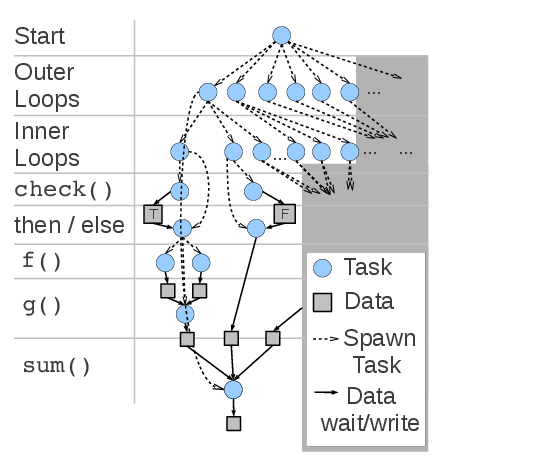
\includegraphics[width=.45\textwidth]{swift_spawngraph}
	\caption{Graph translation of the code\label{fig:swift_exgraph}}
\end{multicols}
\end{figure}

Swift is suitable for Grid.

We found several applications which use Swift.
For instance, \cite{APWXF2011} uses Swift for proteins modelling or \cite{WoiDS2011} for parallel climate data analysis.

\subsubsection{Swift/T}
Swift/T \cite{WAWKL2013} is a new implementation of Swift dedicated to HPC.
It translates the Swift script into a MPI program using Turbine \cite{WAMLK2012} and ADLB (Asynchronous Dynamic Load Balancer) \cite{LusPB2010} libraries.
Turbine is a Tcl library that assemble MPI, ADLB and the Turbine dataflow library.
ADLB is a software library designed to build scalable parallel programs.

Swift/T has two main level of programming : the Swift script and the Leaf functions.
The Swift parallel script correspond to the high grain graph and the leaf functions to the tasks.
The heavy computations are located in the leaf functions.
Since Swit/T uses Swift scripts, the variable assignments and the expression of the parallelism works the same way.

There is three types of leaf functions in Swift/T :
\begin{enumerate}
	\item Extension functions : Tcl (language used in Turbine) or native code functions like C, C++, Fortran or MPI (possibility to call them as parallel functions).
	These functions primarily operate on in-memory data, and are appropriate for high-performance computing.
	\begin{lstlisting}[basicstyle=\ttfamily, tabsize=3, frame=single, language=C, caption=C function\label{lst:swift_cfunc}]
	#include <stdio.h>
	#include <stdlib.h>

	double* b(double* v, int length) {
	  int i;
	  double sum = 0.0;
	  printf("length: %i\n", length);
	  for (i = 0; i < length; i++) {
	    sum += v[i];
	  }
	  printf("sum: %f\n", sum);
	  double* result = malloc(sizeof(double));
	  result[0] = sum;
	  return result;
	}
	\end{lstlisting}
	Listing \ref{lst:swift_cfunc} is the code of the \textit{b} function used in the example\footnote{\url{http://swift-lang.github.io/swift-t/leaf.html\#_complete_example_2_simple_c_function}} of a C leaf function.

	\begin{lstlisting}[basicstyle=\ttfamily, tabsize=3, frame=single, caption=Creation of the Tcl package\label{lst:swift_ctclpackage}]
	rm *.o
	swig -module b b.i
	gcc -c -fPIC b.c
	gcc -c -fPIC $TCL_INCLUDE_SPEC b_wrap.c
	gcc -shared -o libb.so b_wrap.o b.o
	tclsh make-package.tcl > pkgIndex.tcl
	\end{lstlisting}
	Listing \ref{lst:swift_ctclpackage} shows how to create the wrapper of the C function which will be called in the Tcl function.

	\begin{lstlisting}[basicstyle=\ttfamily, tabsize=3, frame=single, caption=Tcl wrapper around the C funtion\label{lst:swift_ctclfunc}]
	namespace eval b {
	    # v is formatted as a Turbine blob a list of [ pointer length ]
	    # The pointer is a simple Tcl integer
	    # The length is the byte length
	    proc b_tcl { v } {

	        # Unpack the list
	        set ptr [ lindex $v 0 ]
	        set len [ lindex $v 1 ]

	        # Get the number of numbers to sum
	        set count [ expr $len / [ blobutils_sizeof_float ] ]

	        # Convert the pointer number to a SWIG pointer
	        set ptr [ blobutils_cast_int_to_dbl_ptr $ptr ]

	        # Call the C function
	        set s [ b $ptr $count ]

	        # Pack result as a Turbine blob and return it
	        set r [ blobutils_cast_to_int $s ]
	        return [ list $r 8 ]
	    }
	}
	\end{lstlisting}
	Listing \ref{lst:swift_ctclfunc} shows how to use the C function inside a Tcl function.
	This Tcl function is used in the Swift application.
	Listing \ref{lst:swift_cswiftapp} shows how to call a Tcl function from a Swift application.

	\begin{lstlisting}[basicstyle=\ttfamily, tabsize=3, frame=single, caption=Call of the Tcl wrapper by a Swift application\label{lst:swift_cswiftapp}]
	import blob;
	import io;

	(blob sum) b(blob v) "b" "0.0"
	[ "set <<sum>> [ b::b_tcl <<v>> ]" ];

	file data = input_file("input.data");
	blob v = blob_read(data);
	blob s = b(v);
	float sum[] = floats_from_blob(s);
	printf("sum (swift): %f", sum[0]);
	\end{lstlisting}
	\item app functions: Functions that call to a command-line program (the shell).
	These functions primarily operate on files, and are appropriate for ordinary workflows.
	\item External scripting functions: Functions that call into an in-memory interpreter in another scripting language, such as Python (Listing \ref{lst:swift_pythonswift}), R (Listing \ref{lst:swift_Rswift}), or \textbf{Julia} (Listing \ref{lst:swift_juliaswift}).
	\begin{lstlisting}[basicstyle=\ttfamily, tabsize=3, frame=single, caption=Call of python code by a Swift application\label{lst:swift_pythonswift}]
	import io;
	import python;
	import string;

	global const string numpy = "from numpy import *\n\n";

	typedef matrix string;

	(matrix A) eye(int n)
	{
	  string command = sprintf("repr(eye(%i))", n);
	  matrix t = python_persist(numpy, command);
	  A = replace_all(t, "\n", "", 0);
	}

	(matrix R) add(matrix A1, matrix A2)
	{
	  string command = sprintf("repr(%s+%s)", A1, A2);
	  matrix t = python_persist(numpy, command);
	  R = replace_all(t, "\n", "", 0);
	}

	matrix A1 = eye(3);
	matrix A2 = eye(3);
	matrix sum = add(A1, A2);
	printf("2*eye(3)=%s", sum);
	\end{lstlisting}


	\begin{lstlisting}[basicstyle=\ttfamily, tabsize=3, frame=single, caption=Call of R code by a Swift application\label{lst:swift_Rswift}]
	import io;
	import string;
	import R;

	global const string template =
	"""
	  x <- %i
	  a <- x+100
	  cat("the answer is: ", a, "\\n")
	""";

	code = sprintf(template, 4);
	s = R(code, "toString(a)");
	printf("the answer was: %s", s);
	\end{lstlisting}


	\begin{lstlisting}[basicstyle=\ttfamily, tabsize=3, frame=single, caption=Call of  Julia code by a Swift application\label{lst:swift_juliaswift}]
	import io;
	import julia;
	import string;
	import sys;

	start = clock();
	f =
	"""
	begin
	 f(x) = begin
	          sleep(1)
	          x+1
	        end
	 f(%s)
	end
	""";
	s1 = julia(sprintf(f, 1));
	s2 = julia(sprintf(f, 2));
	s3 = julia(sprintf(f, 3));
	printf("julia results: %s %s %s", s1, s2, s3);
	wait (s1, s2, s3) {
	  printf("duration: %0.2f", clock()-start);
	}
	\end{lstlisting}
\end{enumerate}

\section{Analysis and First Evaluation of the Languages}

We introduced three classes of programming models : the currently used message passing libraries, fine grain task based programming models in which tasks run on one thread or process and large grain task based programming models in which tasks are distributed and parallel and run on multiple processes.
We studied several task based programming models in each category in detail.
In particular, we studied the properties of HPX, PaRSEC, TensorFlow, Legion, Regent, YML+XMP, Swift and Pegasus.

HPX is a task based programming model.
The tasks are run as lightweight processes on the resources managed by HPX runtime.
The data and the tasks can be transfered across distributed nodes.
It uses modern C++ which starts to be used more often in HPC applications.
It extends C++ future-based (tasks) multi-threaded programming to distributed.
Moreover, HPX is very close to C++ standards so it provides an interface which is supported and documented.
Those are the points for which we are choosing HPX.

PaRSEC is a runtime which manages data and launches tasks.
It also provides several DSLs to define and implement tasks.
Two DSLs are already available.
They allow the user to describe the dependencies between the tasks and how the tasks are implemented.
PaRSEC has good performances compared to the one obtained with HPX as shown in \cite{GurhP2020} .

YML+XMP is a distributed and parallel task based programming model where each task is also distributed and parallel.
This programming has been selected because it has two level of programming, the graph which is the high level and the parallel and distributed task which is the second level.
\cite{GurhP2020} shows that YML+XMP has a better scalability compared to the other programming models.
However, the performances of YML+XMP are its weak points due the use of the file system to perform the communications.
YML+XMP is not the only programming model to use is to make the communications.
Indeed, Pegasus also use files to transfer data from a task to the others.

Legion will not be used due to its way of defining tasks via a tree of tasks which is less natural than a graph of tasks.
Moreover, Legion verbose API is difficult to use.
Finally, Legion performances with the default data mapper are not as good as the performances obtained with the other languages as shown in \cite{GurhP2020} while using Regent to generate Legion code.
Therefore, Regent will not be used too.


TensorFlow is focused in Machine Learning and Neural Networks.
It is well adapted to train models and to process data with those models.
It offers a high level API to easily create and train models.
In TensorFlow, the Operation is the main way to apply computations on data stored into Tensors aside the Machine Learning API.
However, Operations can only be implemented by adding it directly into TensorFlow code and by recompiling it.
Therefore, it is not well adapted to other kind of applications and will not be used to implement the Kirchhoff Migration.
%TODO not used for which application ?

CnC does not seem to be used a lot and does not seem maintained anymore.
Thus, CnC will not be used to implement applications.

OmpSs uses the same kind of approach as OpenMP.
It uses directives to parallelize sections of code.
However, the execution model is different but it still produces multi-threaded applications whereas distributed programming models are considered in this study.

Swift is a parallel programming model where the tasks are also parallel and distributed.
However, the data are sent to the tasks as blobs, an array of bytes, which is copied in each process of the tasks.
Therefore, the distribution of the data is not optimal since each process of the task has a copy of the whole data instead of a part of it.
Furthermore, the user has to write interface with the libraries that will be used as tasks.
This interface consists of several Tcl wrappers and automatic interface generation.
This process could be could be fully hidden from the user.
Swift will not be studied further fo those reasons.

\section{Application Deployment with Containers}
Applications which use an uncommon software stack may be difficult to deploy on supercomputers.
YML+XMP is an example of such an application.
It depends on libraries that are not commonly installed on supercomputers like \textit{Util}, a library implemented for YML or \textit{OmniRPC} and the \textit{omnicompiler} which are used to compile and launch parallel and distributed XMP based tasks.
Moreover, XMP tasks are compiled into an application which is executed by YML scheduler through \textit{OmniRPC} with \textit{MPI\_Comm\_spawn}.
Very few MPI implementations support \textit{MPI\_Comm\_spawn} as used by YML and \textit{OmniRPC} so installing the whole software stack with the right versions and support on a supercomputer is challenging.
Furthermore, containerization technologies are not well supported yet on current supercomputers especially for distributed applications.
The integration of those technologies on supercomputers is a interesting opportunity to make the deployment of complex software stacks easier.

To address this deployment issue, we created containers which can hold the recipe to compile and install YML+XMP for a given architecture.
These containers can be built on the supercomputers if the user has the rights to do so or build locally then sent on the supercomputer for execution.
The build recipe are used to create a lightweight system image containing all the libraries needed to run the applications.
The YML+XMP containers are made with Docker and Singularity which are lightweight virtualization systems.
They allow to build and install applications in a controlled environment similar to virtual machines but lighter and with better performances.

Moreover, the use of container images is not limited to deployment on supercomputers.
They can also be used to easily access complex software stack on the developers machines without having to fully install it.
Therefore, they can gain in productivity and use the same environment as the one used on the supercomputer to develop the application locally.
Finally, containers can be used to replicate software stack and application development on other supercomputers and reproduce experiments on machine which support containers.


% chapter transition
\paragraph{}
We introduced several task based programming models and how to use them to implement task, define dependencies, register distributed data and how to execute the graph of tasks.
This classification and the informations on how to use the programming models to define tasks, express dependencies as well as register data are a contribution of this dissertation.
We also selected YML+XMP, PaRSEC and HPX to implement out applications and make out experiments.
These programming models will be used in the following chapter to experiment on dense linear algebra.
We will discuss our numerical experiments with the LU factorization and the solution of dense linear systems.
	\chapter{Task-Based, Parallel and Distributed Dense Linear Algebra Applications \label{chap:exp_dense}}
\graphicspath{{chapters/exp_dense/}}

\section{Task-Based Methods and Algorithms}


Let $A$ be a block matrix of size $np \times np$ and $p \times p$ blocks so each block is of size $n \times n$ .
Let $b$ and $x$ be block vectors of size $np$ and $p$ blocks so each block is of size $n$.
The goal here is to solve the linear system $Ax=b$.

In the following algorithms, $A_{i,j}^{(k)}$ represents the $k^{th}$ version of the block at the $i^{th}$ row and $j^{th}$ column of the block matrix $A$.
Thus, $b_i^{(k)}$ represents the $k^{th}$ version of the block at the $i^{th}$ row of the block vector $b$.
The algorithm is expressed using assignments on the blocks of $A_{i,j}^{(k+1)}$ and $b_i^{(k+1)}$.
They consist on operations on blocks like matrix matrix product, inversion of a matrix and matrix vector product.
Each assignment will correspond to a task in the implementation of the algorithms so the number of task will correspond to the number of assignments.




\subsection{Block-Based Gaussian Elimination to Solve Linear Systems}

\begin{algorithm}[h]
	\DontPrintSemicolon
	\caption{Block-Based Gaussian elimination and back substitution \label{alg:bg_el_data_dep}}
	%\scriptsize
	\For{k \KwFrom 0 \KwTo p-2}{
		(1) $\displaystyle Inv^{(k)} = [A_{k,k}^{(k)}]^{-1}$ \;
		(2) $b_k^{(k+1)} = Inv^{(k)} \cdot b_k^{(k)}$ \;
		\For{j \KwFrom k+1 \KwTo p-1}{
			(3) $\displaystyle A_{k,j}^{(k+1)} = Inv^{(k)} \cdot A_{k,j}^{(k)} $ \;
		}
		\For{i \KwFrom k+1 \KwTo p-1}{
			(4) $b_i^{(k+1)} = b_i^{(k)} - A_{i,k}^{(k)} \cdot b_k^{(k+1)}$ \;
			\For{j \KwFrom k+1 \KwTo p-1}{
				(5) $A_{i,j}^{(k+1)} = A_{i,j}^{(k)} - A_{i,k}^{(k)} \cdot A_{k,j}^{(k+1)}$ \;
			}
		}
	}

	(6) $b_{p-1}^{(p)} = Inv^{(p-1)} \cdot b_{p-1}^{(p-1)}$ \;

	\For{k \KwFrom 1 \KwTo p-1 }{
		\For{i \KwFrom 0 \KwTo p-k-1 }{
			(7) $b_i^{(k+i+1)} = b_i^{(k+i)} - A_{i,p-k}^{(i+1)} \cdot b_{p-k}^{(p)}$ \;
		}
	}
\end{algorithm}

The Gaussian elimination in Algorithm \ref{alg:bg_el_data_dep} solves the system by doing a block triangularization of the block matrix $A$, and by solving the triangular system.
In this algorithm, the number of assignments is $\frac{p^3+3p^2+2p}{3} \sim \frac{p^3}{3}$.
The block-wise Gaussian elimination and back substitution have been implemented using YML/XMP.

For this experiments, the Algorithm \ref{alg:bg_el_data_dep} is expressed as YvetteML graph and the operations on blocks are implemented using XMP.
Each operation is performed on a matrix of a vector which are a subdivision of the global matrices and vectors.
In YvetteML, there are two means to express the parallelism between components : the \textit{par} loop and the \textit{par} statement.
To implement the block-wise Gaussian elimination, we expressed all the call to the components in parallel and we used the event management system of YvetteML to express the dependencies between the tasks.
In the Algorithm \ref{alg:bg_el_data_dep}, we observe that each block i,j at step k of the Gaussian Elimination is updated only once.
Then, it is possible to associated the corresponding tasks to the triplets (i,j,k).
Each task may be launched only when some tasks of the previous steps are completed and when the data are migrated to the allocated computing resource.
Therefore, the dependency graph is equivalent in this case of the precedence between triplets: for example (i,j,k) will always depend of (i,j,l$<$k), for the adequate value of i,j, and k.
If we associate each triplet to a Yvette array of events, each assignment of the block (i,j) at step k in the Algorithm \ref{alg:bg_el_data_dep} have to be preceded by a “wait” expressing the dependence between (i,j,k) and previous triplets.
For the block i of a given step  of the back substitution, we use the same properties.

The XMP components that make the different operations are also written to take advantage of the XMP directives and use the processors allocated by YML to efficiently run the operations on the block matrices.



\subsection{Block-Based Gauss-Jordan Elimination to Solve Linear Systems}

\begin{algorithm}[h]
	\DontPrintSemicolon
	\caption{Block-Based Gauss-Jordan elimination to solve a linear system \label{alg:bgj_data_dep} }
	\For{k \KwFrom 0 \KwTo p-1}{
		(1) $\displaystyle Inv^{(k)} = [A_{k,k}^{(k)}]^{-1}$ \;
		(2) $b_k^{(k+1)} = Inv^{(k)} \cdot b_k^{(k)}$ \;
		\For{j \KwFrom k+1 \KwTo p-1}{
			(3) $\displaystyle A_{k,j}^{(k+1)} = Inv^{(k)} \cdot A_{k,j}^{(k)} $ \;
			\For{i \KwFrom 0 \KwTo p-1}{
				\If{k $\neq$ i}{
					(4) $A_{i,j}^{(k+1)} = A_{i,j}^{(k)} - A_{i,k}^{(k)} \cdot A_{k,j}^{(k+1)}$ \;
				}
			}
		}
		\For{i \KwFrom 0 \KwTo p-1}{
			\If{k $\neq$ i}{
				(5) $b_i^{(k+1)} = b_i^{(k+1)} - A_{i,k}^{(k)} \cdot b_k^{(k+1)}$ \;
			}
		}
	}
\end{algorithm}

\subsection{Block-Based LU factorization}

\begin{algorithm}[h]
	\DontPrintSemicolon
	%\SetAlgoVlined
	\caption{LU Factorization\label{alg:lufact_data_dep}}
	\For{k \KwFrom 0 \KwTo p-2}{
		(1) $\displaystyle Inv^{(k)} = [A_{k,k}^{(k)}]^{-1}$ \;
		\For{i \KwFrom k+1 \KwTo p-1}{
			(2) $\displaystyle A_{i,k}^{(k+1)} = A_{i,k}^{(k)} \cdot Inv^{(k)}$ \;
			\For{j \KwFrom k+1 \KwTo p-1}{
				(3) $A_{i,j}^{(k+1)} = A_{i,j}^{(k)} - A_{i,k}^{(k+1)} \cdot A_{k,j}^{(k)}$ \;
			}
		}
	}
\end{algorithm}

\begin{figure}[h]
	\centering
	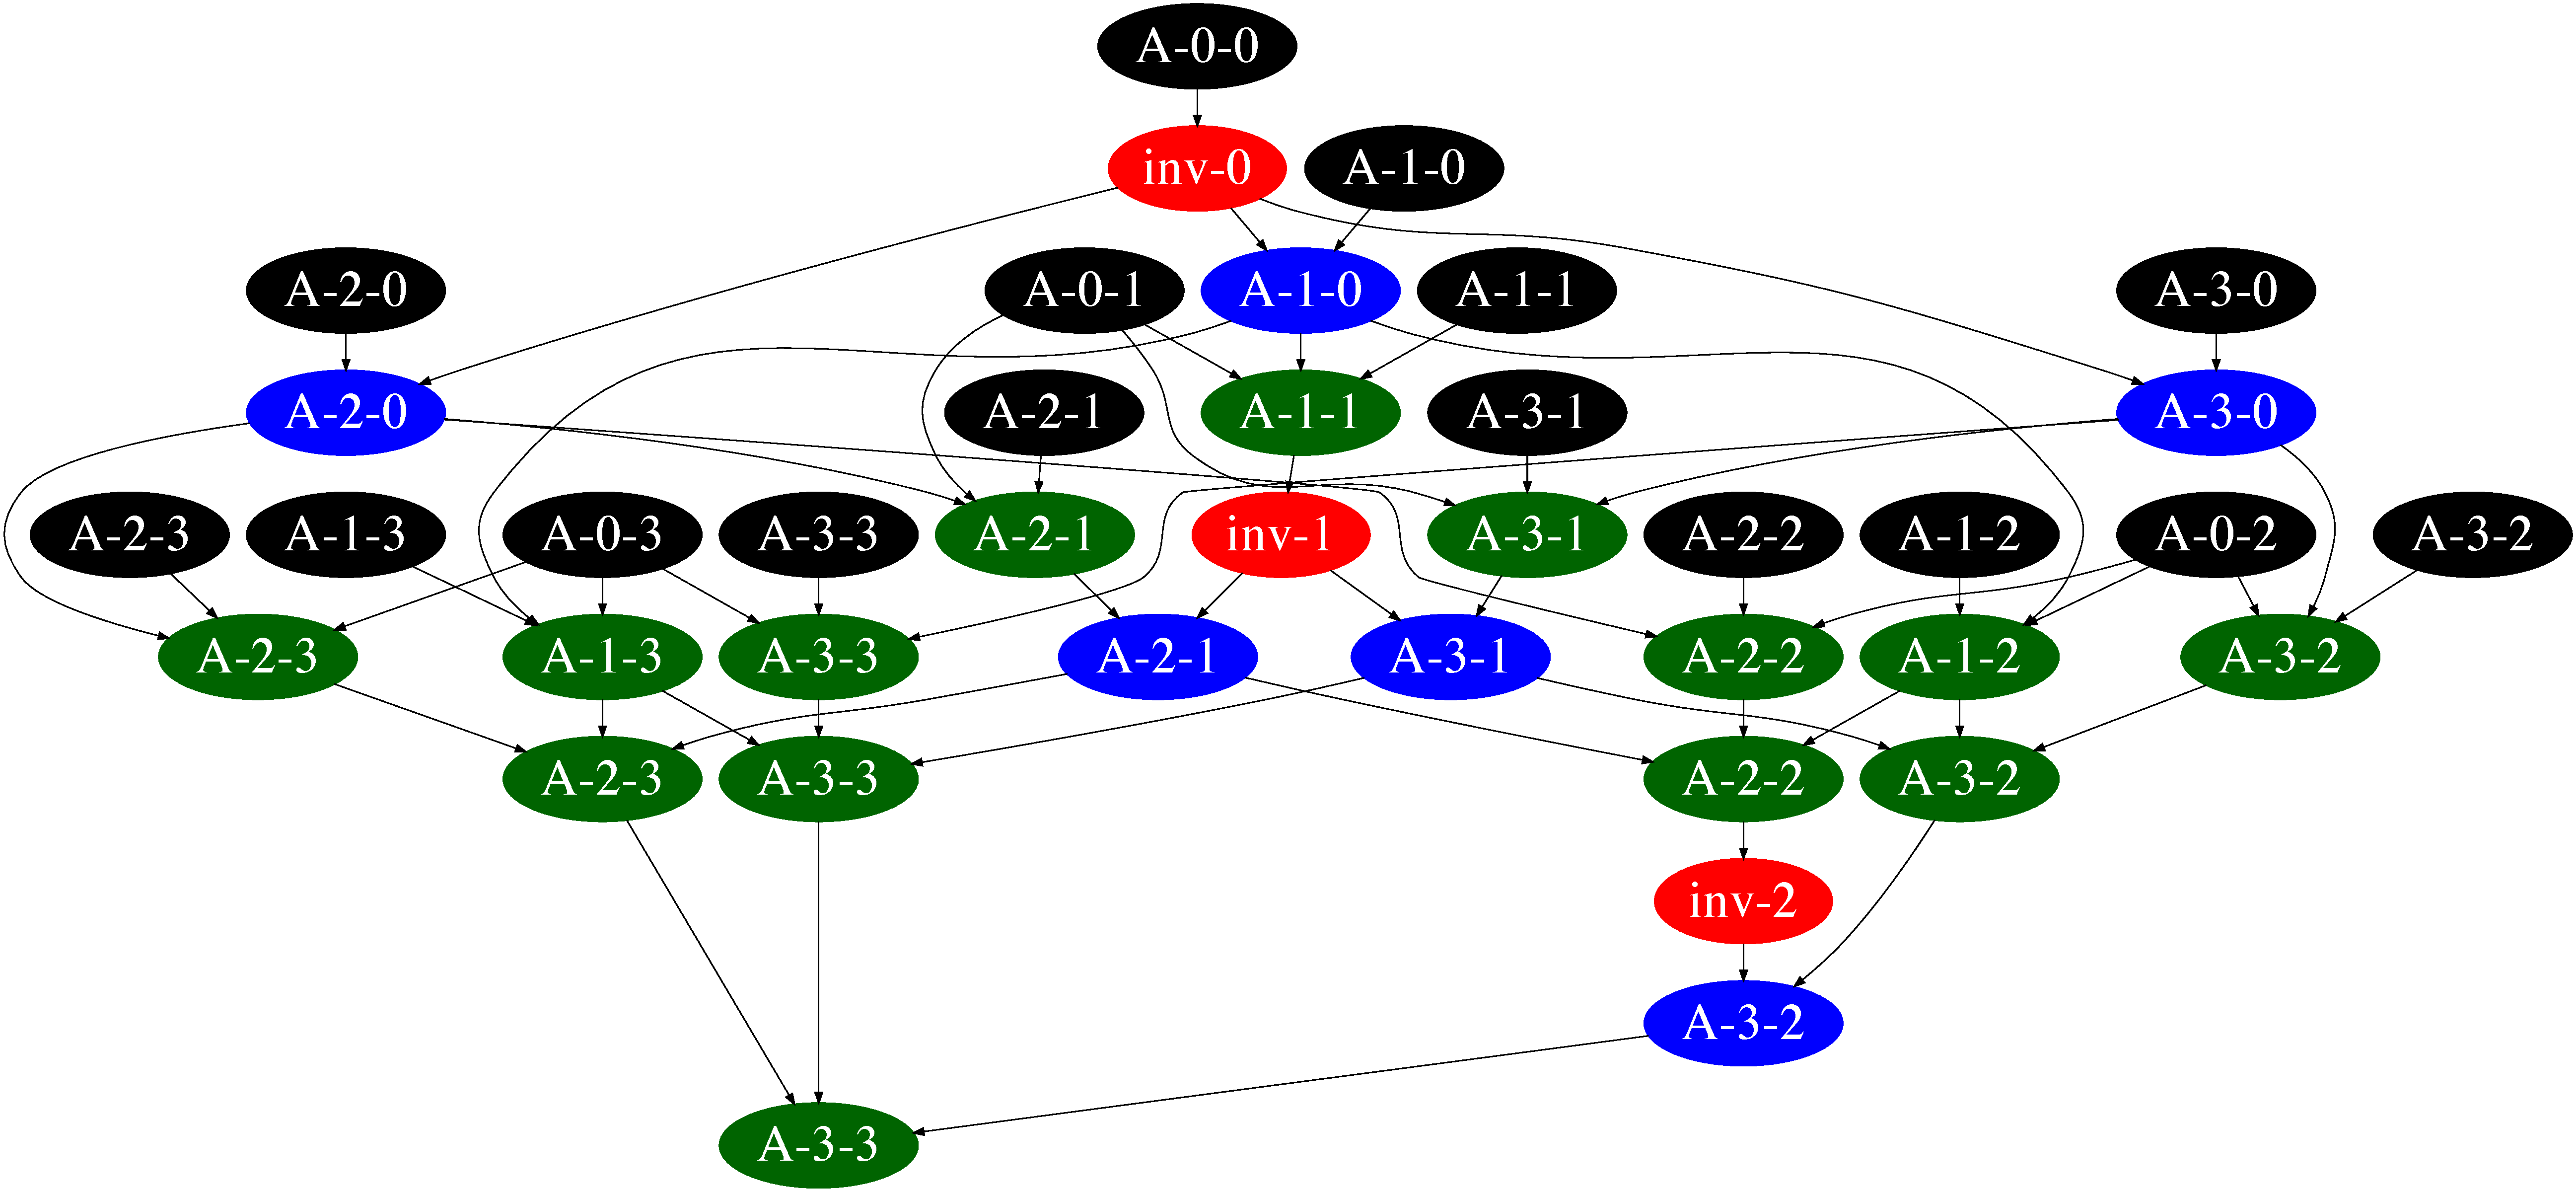
\includegraphics[width=\textwidth]{lu_graph_n4}
	\caption{Block-based LU factorization graph for p = 4\label{fig:graph_lu}}
\end{figure}

\subsection{Block-Based LU factorization to Solve Linear Systems}


\begin{algorithm}[h]
	\DontPrintSemicolon
	%\SetAlgoVlined
	\caption{Solution of a linear system with a block-based LU factorization\label{alg:lufact_sls_data_dep}}
	\For{i \KwFrom 0 \KwTo p-2}{
		\For{j \KwFrom i+1 \KwTo p}{
			(5) $b_j^{(i+1)} = b_j^{(i)} - A_{j,i}^{(i+1)} \cdot b_i^{(p)}$ \;
		}
	}
	\;
	\For{k \KwFrom p-1 \KwTo 0 \KwStep -1}{
		(6) solve $b_{k}^{(p)} = A_{k,k}^{(k)} \cdot b_k^{(p-1)}$ \;
		\For{i \KwFrom 1 \KwTo k-1}{
			(7) $b_i^{(p-k+i)} = b_i^{(p-k+i-1)} - A_{i,k}^{(i)} \cdot b_k^{(p)}$ \;
		}
	}
\end{algorithm}


\section{Numerical Experiments on Linear systems}

In the first place, the multi-level programming YML/XMP will be compared to XMP on the K computer where OmniRPC and XMP are installed.
Then, YML/XMP and XMP will be compared to ScaLAPACK and the implementation of the resolution of a dense linear in MPI on Poincare.


\subsection{Experiments on the K computer}

\subsubsection{The supercomputer}
In this section, the tests were performed on the K Computer from Riken AICS in Kobe, Japan.
This supercomputer was manufactured by Fujitsu.
There is 88,128 compute nodes containing an eight-core SPARC64 VIIIfx processor and 16 Go of memory.
The network is based on Tofu interconnect.

\subsubsection{Resolution of a linear system of size 16384 on 1024 cores}
This experiment consists in solving a dense linear system of size 16384 with the block-wise Gaussian elimination with YML/XMP.
The matrix is already generated and each YML task has to load its data from the file system, makes the computations on the data then saves its results to the file system.
The matrix is stored by blocks and each task makes an operation on blocks of the global matrix.
YML expresses the operations on blocks while XMP is used to implement them.
We experiment different numbers of blocks and numbers of cores per task.
Only one process runs on each core.
We used from $1\times 1$ block to $16\times 16$ blocks with tasks from 16 to 512 cores out of the 1024 cores of the K Computer allocated to each run.
The time needed to solve the linear system without the generation of the matrix is evaluated in this study.

\begin{figure}[h]
	\caption{Resolution of linear system using Gaussian elimination + back substitution (size of 16384) on the K computer\label{fig:K_g}}
	\centering
	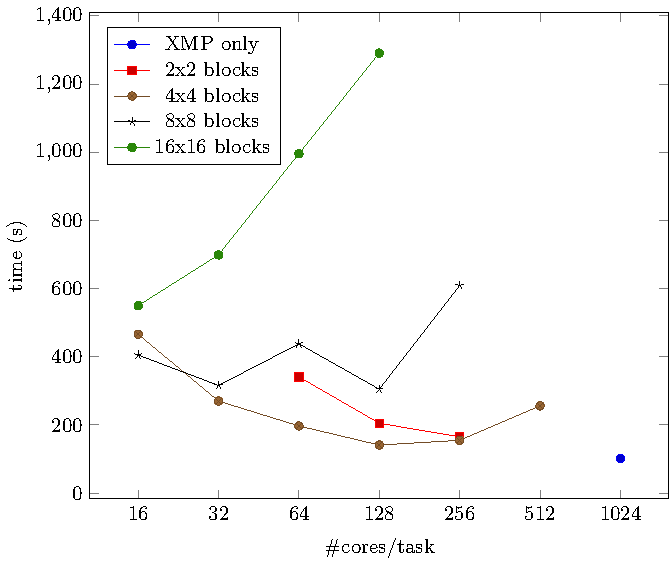
\includegraphics[width=.6\textwidth]{figK-g-16k.pdf}
\end{figure}

\begin{figure}[h]
	\caption{Resolution of linear system using Gauss-Jordan elimination (size of 16384) on the K computer\label{fig:K_gj}}
	\centering
	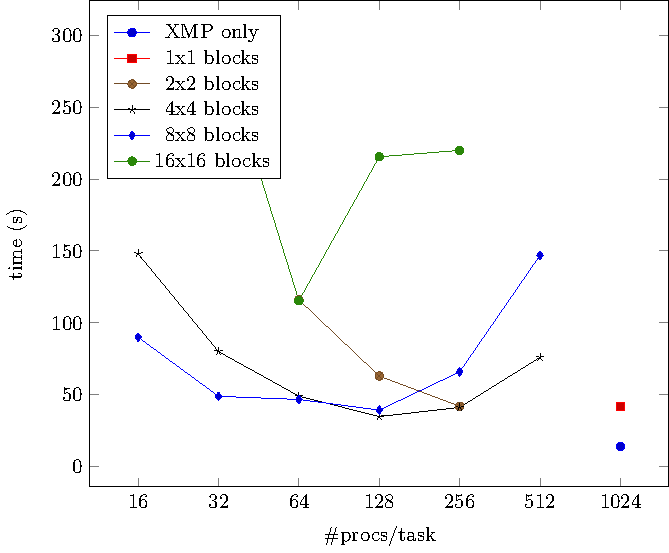
\includegraphics[width=.6\textwidth]{figK-gj-16k.pdf}
\end{figure}

\begin{figure}[h]
	\caption{Resolution of linear system using LU factorization + forward and backward substitution (size of 16384) on the K computer\label{fig:K_lu}}
	\centering
	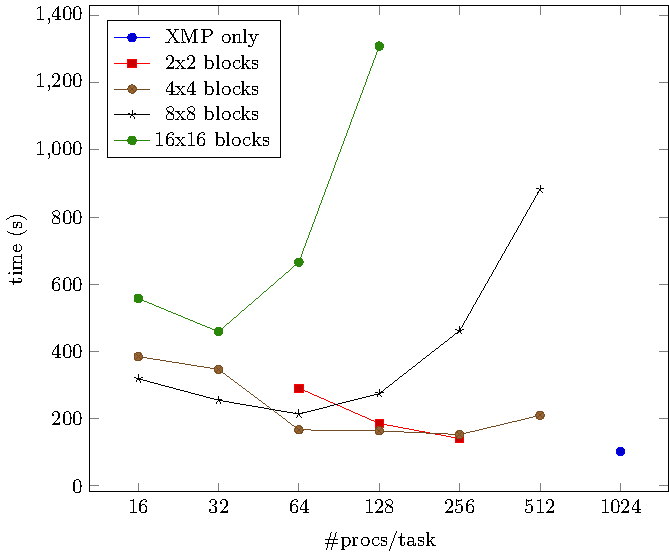
\includegraphics[width=.6\textwidth]{figK-lu-16k.pdf}
\end{figure}

In the Figure \ref{fig:K_g}, we observe the impact of the number of blocks and the number of cores per task on the execution time for the Gaussian elimination.
We also observe the same kind of behavior for the two other applications using different methods to solve the same linear system : the Gauss-Jordan elimination in Figure \ref{fig:K_gj} and the LU factorization in Figure \ref{fig:K_lu}.
We also compare the YML/XMP application to a XMP implementation of the resolution of a linear system through the non-block Gaussian elimination.
We reached the best time in YML/XMP with $4 \times 4$ blocks and 128 cores per task for 141s while the XMP code took 102s.

\textbf{The number of blocks} determines the number of tasks in the application.
For $p \times p$ blocks, there are $\frac{p^3+3p^2+2p}{3}$ tasks in the Gaussian elimination application.
Thus, the application needs to have enough tasks to contain enough parallelism without decreasing to significantly the execution time of each task.
The number of blocks also influences the size of the block since the size of a block is $16384/p \times 16384/p$ values for the matrices and $16384/p$ values for the vectors in the case of a linear system of size 16384.
If the number of blocks is large then the size of the block is small and the tasks on the blocks will be quick.
In the opposite, a small number of blocks implies a large size of blocks so the task will be longer since it will need more operations.
Moreover, if the application has too many tasks, the tasks execution will not compensate the overhead from YML.

\textbf{The number of cores per task} sets the number of YML workers since all the tasks use the same amount of cores and the total number of cores is fixed.
Each worker launches a task at a time so there is the same number of parallel tasks as there is number of workers.
For instance, we use 1024 cores in total and 128 cores per task so there are 8 parallel tasks maximum.
The number of blocks needs to be high enough to use all the workers most of the time or there is unused compute power and the application will take more time.
The number of cores per task also influences the speed of the execution of a task since a large number of cores will have more compute power but will also introduce more communications between cores.
On the opposite, a small number of cores will induce less communications but the task will take more time.

\textbf{A compromise} between the number of blocks and the number of cores per task is mandatory to obtain good performances.
The number of blocks gives enough tasks so there is a great number of those tasks that can be run in parallel and determines the size of the data in the task.
The number of cores per task gives the number of parallel workers and the execution time of each task.
The good compromise gives enough parallel tasks so the workers are busy most of the time and the execution time of the tasks is balanced with the size of the data that need to be treated.
It results in applications that use efficiently the available resources.

\begin{table}[h]
	\caption{Execution time (s) to solve a linear system on the K computer with 1024 cores\label{tab:K_1024p_16384n}}
	\centering
	\begin{tabular}{ccccc}
		                         &      \multicolumn{3}{c}{YML/XMP}      &  XMP   \\
		                         &    blocks    & cores/task & best time &        \\ \hline
		  Gaussian elimination   & $4 \times 4$ &    512     &  141.02   & 102.82 \\
		Gauss-Jordan elimination & $4 \times 4$ &    512     &  138.931  & 229.74 \\
		    LU factorization     & $4 \times 4$ &    512     &  141.221  & 103.07
	\end{tabular}
\end{table}


As shown in Table \ref{tab:K_1024p_16384n}, XMP is faster than YML+XMP in solving the linear system without considering the method used.
However, the Gauss-Jordan elimination elimination performs better in YML+XMP than in XMP whereas the Gaussian elimination and the LU factorization are faster in XMP than their counterpart in YML+XMP.
Moreover, the Gauss-Jordan elimination is more compute and communication intensive compared to the LU factorization and the Gaussian elimination and thus, takes more time than the other two in XMP.
Indeed, the operations of the Gauss-Jordan elimination are a bit different from the Gaussian elimination since the operations above the diagonal in the Gaussian elimination are also performed below the diagonal in the Gauss-Jordan elimination.
Hence, there is no resolution of triangular system and is directly solved.
On the other hand, the Gauss-Jordan elimination in YML+XMP has a similar execution time compared to the Gaussian elimination and the LU factorization in YML+XMP.
We think that the number of cores is too small thus the overhead from YML doesn't compensate for direct communications across all the cores in the Gaussian elimination and the LU factorization although it works well for the Gauss-Jordan elimination.
Then, we tried to solve a bigger system on a higher number of cores.


\subsubsection{Resolution of a linear system of size 32768 and 65536 on 8096 cores}
We also made experiments on larger systems with more cores : 32768 and 65536 on 8096 cores.
The Table \ref{tab:K_8096p} summarize the execution times obtained.

\begin{table}[h]
	\caption{Execution time (s) to solve a linear system on the K computer with 8096 cores\label{tab:K_8096p}}
	\centering
	\begin{tabular}{cccccc}
		                                          & Size  &      \multicolumn{3}{c}{YML/XMP}      &   XMP    \\
		                                          &       &    blocks    & cores/task & best time &          \\ \hline
		  \multirow{2}{*}{Gaussian elimination}   & 32768 & $4 \times 4$ &    512     &   276.8   &  508.5   \\
		                                          & 65536 & $8 \times 8$ &    512     &    690    &   2512   \\ \hline
		\multirow{2}{*}{Gauss-Jordan elimination} & 32768 & $4 \times 4$ &    512     &  285.12   & 615.868  \\
		                                          & 65536 & $8 \times 8$ &    512     &  792.737  & 2970.393 \\ \hline
		    \multirow{2}{*}{LU factorization}     & 32768 & $4 \times 4$ &    512     &  332.35   & 505.412  \\
		                                          & 65536 & $8 \times 8$ &    512     &  881.032  & 2306.163
	\end{tabular}
\end{table}

In this experiment, we increased the size of the system and the number of cores.
In this case, YML/XMP performed better than XMP alone for the two different size for each application.
This is mainly due to the fact that YML doesn't make any global communications like broadcast over all the cores allocated to the application.
Indeed, each task runs on a subset of the resources and the communications between tasks are made through the data server.
Although, the overhead of YML is noticeable (this will be discussed in the next section), YML+XMP runs faster than XMP alone on 8096 cores of the K Computer.
Thus YML+XMP and the task programming languages may be a good solution to develop and execute complex applications on huge numbers of cores on large super-computers.

In this case, where the size of the problem and the number of computational resources has increased, the Gaussian elimination in YML+XMP is noticeably faster than the LU factorization and the Gauss-Jordan elimination in YML+XMP whereas the three of them were equivalent in the previous case.
Moreover, the Gaussian elimination and the LU factorization have almost the same number of tasks but the Gaussian elimination executes faster.
Indeed, the critical path of the Gaussian elimination is shorter than the critical path of the LU factorization due to the fact that, in the LU factorization, there is two triangular systems to solve while there is only one in the Gaussian elimination.
The Gauss-Jordan elimination also performs better than the LU factorization although there is more computation but the critical path is even shorter than the critical path of the Gaussian elimination.
We think that with greater sizes of problem and number of computational resources, the discrepancy between the LU factorization and the Gaussian elimination will increase whereas it will decrease between the Gauss-Jordan elimination and the Gaussian elimination.
The Gauss-Jordan elimination may even execute faster than the Gaussian elimination at some point.


We compared YML/XMP to XMP for several cases on the K computer to evaluate the multi-level distributed/parallel programming associated to the studied programming paradigm on such supercomputer, even if the system of these machines does not yet propose smart scheduling.
As YML and XMP were introduced by authors of this paper, as the OmniRPC middleware used fore these experiments, we have to evaluate such programming on a more general cluster and compare it to more classic end-user programming.
Then, in the next section, we compare YML/XMP and XMP to ScaLAPACK and our MPI implementation of the resolution of a dense linear system on Poincare, an IBM cluster.


\subsection{Experiments on Poincare\label{sec:exp}}

\subsubsection{The cluster}
The tests were performed on Poincare, the cluster of \textit{La Maison de la Simulation} in France.
It is an IBM cluster mainly composed of iDataPlex dx360 M4 servers, hosted at the CNRS supercomputer centre in Saclay, France.
There is 92 compute nodes with 2 Sandy Bridge E5-2670 processors (8 cores each, so 16 cores per nodes) and 32 Go of memory.
The file system is constituted of two parts : a replicated file system with the homes of the users and a scratch file system with a faster access from the nodes.
The network is based on QLogic QDR InfiniBand.

\subsubsection{The experiments}
We performed the same tests on YML/XMP as on the K Computer.
We also compared those results to ScaLAPACK, to our custom MPI implementations and $1\times 1$ block in YML/XMP.

In the case of $1\times 1$ block, there is only one assignment performed on a dense linear system with a XMP component.
The component which runs the resolution of linear system is developed using XMP so we can evaluate the time that YML need to schedule the data, import it, run the XMP application then export the data.
The data is loaded from the file system.
This is the worst case for YML since it does not use the advantages of YML like scheduling and high grain parallelism.

We also compare the YML/XMP implementation of the Gaussian elimination, the Gauss-Jordan elimination and the Lu factorization to a XMP and a MPI implementations.
Finally, we also compare to a ScaLAPACK implementation of the resolution of a dense linear system through LU factorization.
In each case, we load the data from disk using MPIIO then we solve the linear system and save the result vector on disk using MPIIO.

In the MPI case, we used a cyclic distribution of the columns to keep a good load balancing in the cores.
Moreover, we created a distributed cyclic array type in MPI in order to use it with MPIIO.
This results in a matrix well stored by columns in the file.
The cyclic distribution takes more time since it is easier to store the data without reordering them during the import/export.

\subsubsection{The results}

\begin{figure}[h]
	\caption{Resolution of linear system using Gaussian elimination + backward substitution (size of 16384 on the left and 32768 on the right) on Poincare\label{fig:g1}}
	\centering
	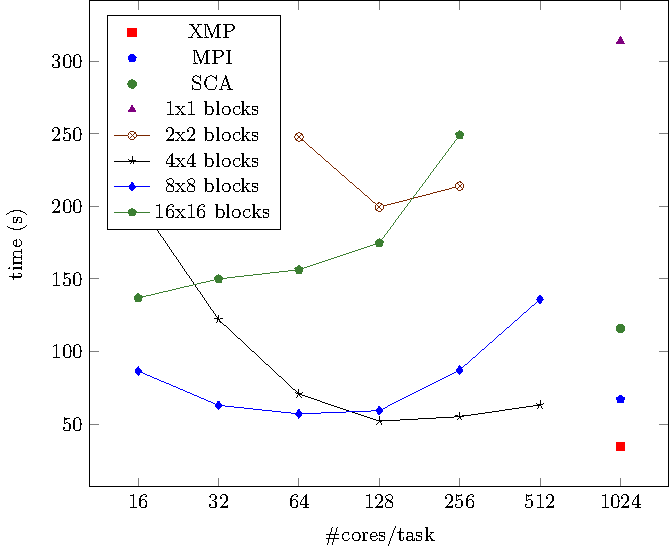
\includegraphics[width=.49\textwidth]{fig-g-16k.pdf}
	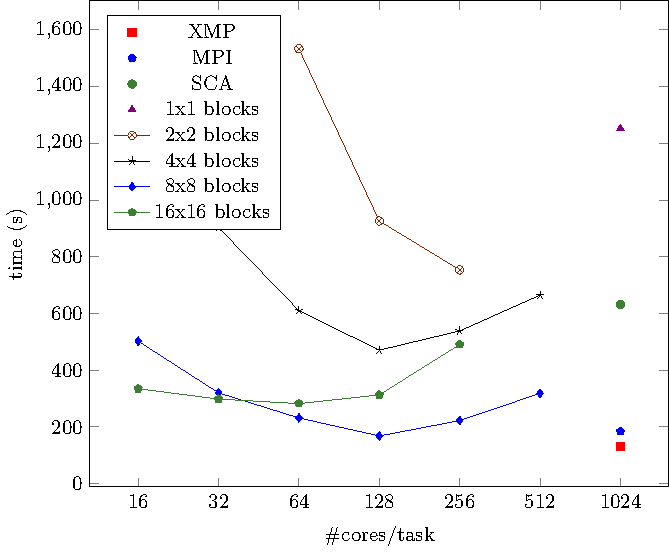
\includegraphics[width=.49\textwidth]{fig-g-32k.pdf}
\end{figure}

The Figure \ref{fig:g1} shows the performances to solve a linear system of size 16384 and 32768 by the block Gaussian elimination and the block resolution of the resulting triangular system using YML/XMP.
The best execution time for YML/XMP is obtained with $4 \times 4$ blocks and 128 cores per tasks for 51.9s for the size of 16768.
The $1 \times 1$ block case with YML/XMP takes more time than the XMP only program (34.5s vs 313s).
We also obtain similar results with the LU factorization (see Figure \ref{fig:lu_poincare}) and the Gauss-Jordan elimination (see Figure \ref{fig:gj}).

The Table \ref{tab:best_time_poincare} gives a summary of the results obtained with the different programming paradigms.
We have the values for two sizes of system 16384 and 32768.
Moreover, for the MPI, XMP and ScaLAPACK cases, we also have the time spent in computation between parenthesis.
The rest of the time is spent in IO to load and save the data as it is done for each component in YML/XMP.

\begin{figure}[H]
	\caption{Resolution of linear system using LU factorization + backward and forward substitution (size of 16384 on the left and 32768 on the right) on Poincare\label{fig:lu_poincare}}
	\centering
	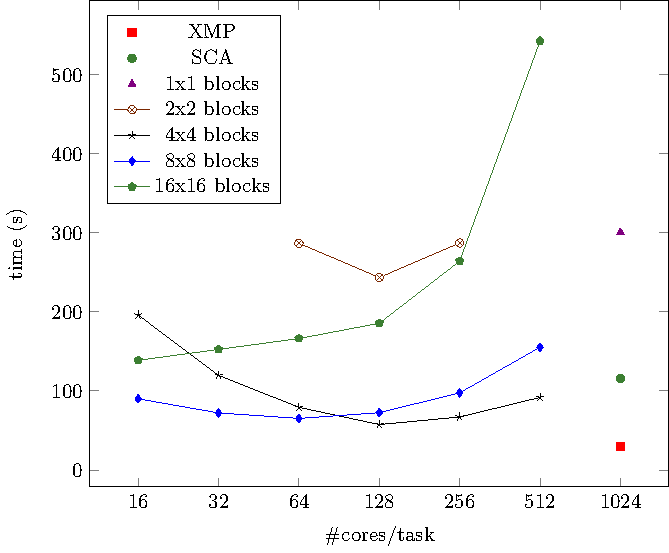
\includegraphics[width=.49\textwidth]{fig-lu-16k.pdf}
	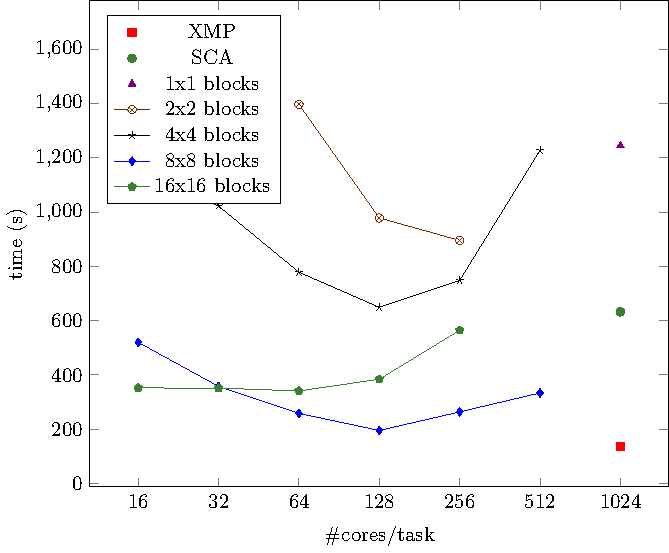
\includegraphics[width=.49\textwidth]{fig-lu-32k.pdf}
\end{figure}

\begin{figure}[h]
	\caption{Resolution of linear system using Gauss-Jordan elimination (size of 16384 on the left and 32768 on the right) on Poincare\label{fig:gj}}
	\centering
	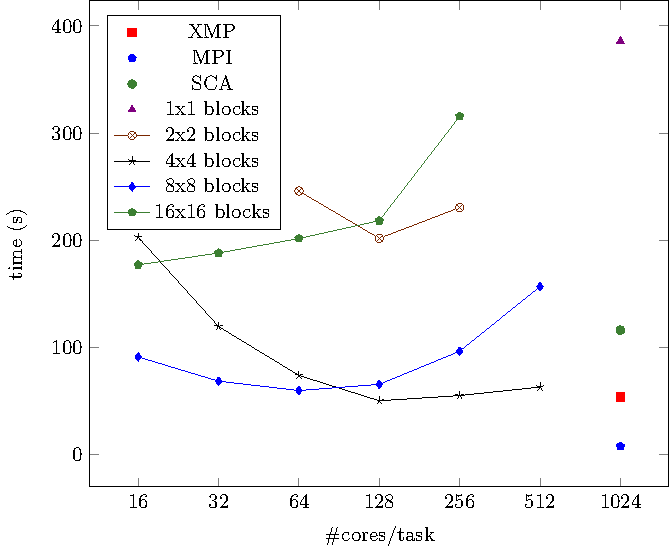
\includegraphics[width=.49\textwidth]{fig-gj-16k.pdf}
	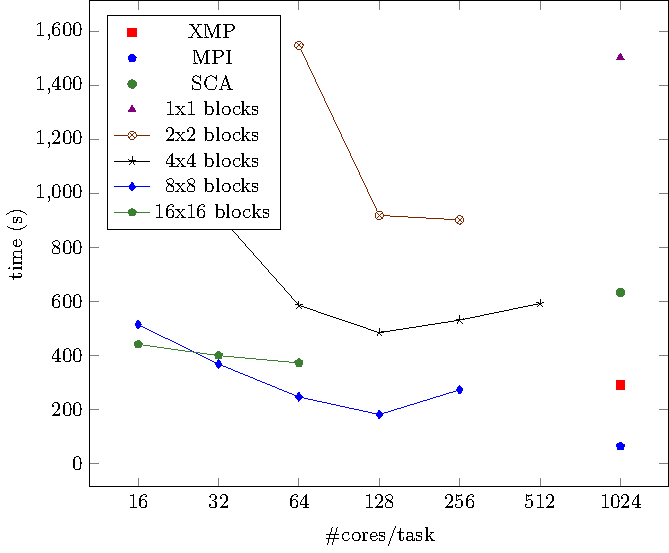
\includegraphics[width=.49\textwidth]{fig-gj-32k.pdf}
\end{figure}


With the Gauss-Jordan method, YML/XMP runs faster than XMP on Poincare for the two sizes of systems and the difference increases with the size of the system.
We observe the same effect of balance between the number of cores per task and the number of blocks as we seen previously.
The parallelism inside the Gauss-Jordan elimination is greater so the task parallel programming paradigm take advantage of this parallelism to execute the application.
Moreover, there is no global communications in YML/XMP but they are widely used in XMP so the increase of operations from the Gaussian elimination to the Gauss-Jordan elimination is more impacting in XMP.
Our MPI implementation is unexpectedly quite fast on a system of size 163824 but ScaLAPACK is more efficient in term of computation for the 32768 system.
Finally, the Gaussian elimination performed almost two times better on XMP than the Gauss-Jordan elimination but the two methods got very close results on YML/XMP.

\begin{table}[h]
	\caption{Execution time (s) to solve a linear system\label{tab:best_time_poincare}}
	\centering
	\begin{tabular}{cccc}
		                                          &           Language           &    16384     &      32768      \\ \hline
		  \multirow{5}{*}{Gaussian elimination}   &     YML/XMP (best case)      &     51.9     &      168.3      \\
		                                          & YML/XMP ($1 \times 1$ block) &     313      &      1252       \\
		                                          &             MPI              & 66.9 (60.6)  &  183.7 (161.9)  \\
		                                          &             XMP              & 34.5 (32.7)  &  131.4 (129.6)  \\
		                                          &          ScaLAPACK           & 115.9 (18.5) &  632.1 (55.6)   \\ \hline
		    \multirow{4}{*}{LU factorization}     &     YML/XMP (best case)      &    57.508    &      194.8      \\
		                                          & YML/XMP ($1 \times 1$ block) &    300.75    &      1244       \\
		                                          &             XMP              & 29.9 (29.4)  & 136.264 (135.6) \\
		                                          &          ScaLAPACK           & 115.9 (18.5) &  632.1 (55.6)   \\ \hline
		\multirow{5}{*}{Gauss-Jordan elimination} &     YML/XMP (best case)      &     49.9     &       180       \\
		                                          & YML/XMP ($1 \times 1$ block) &     385      &      1502       \\
		                                          &             MPI              &  7.4 (4.5)   &    62.1 (59)    \\
		                                          &             XMP              & 53.4 (52.8)  &   289.7 (289)   \\
		                                          &          ScaLAPACK           & 115.9 (18.5) &  632.1 (55.6)
	\end{tabular}
\end{table}

In this case, we globally see the same results although, the Gauss-Jordan elimination has more operations and uses more communications than the Gaussian elimination.
We run faster with YML/XMP than XMP due the parallelism of the method being highly exploited by the parallel task paradigm and not using any global communications.
The efficiency of the YML/XMP depends on the method implemented since the Gaussian elimination and the Gauss-Jordan elimination performed quite close on the two sizes of system while the Gauss-Jordan elimination has a significantly higher number of operations.
The methods with a high parallelism are very suited to the parallel task programming paradigm and perform very well compared to XMP and ScaLAPACK.
The format of the data stored in files by the data server (row-wise) wasn't suited for the distribution of the data used by ScaLAPACK so it didn't performed well as an application.
The use of a better distribution of the data in ScaLAPACK and a data server making IO with the file system in YML/XMP may have shown better performances but YML/XMP and the parallel task programming paradigm show that, even with a high overhead for each task, we can get good performances.


\subsubsection{A comparison between YML/XMP, XMP, MPI and ScaLAPACK}

We can see a huge overhead in YML/XMP for $1 \times 1$ blocks compared to XMP alone in the Table \ref{tab:best_time_poincare}.
This is the case for the two sizes of system and the three applications.
Thus, we can expect a pretty huge overhead from YML for each component.
But, the most favorable case in YML/XMP solve the linear system in 51.9s whereas XMP took 34.5, MPI took 66.9s and ScaLAPACK took 115.9s.
Although, from the 66.9s only 60.6s is spent on computing.
The rest is spent in MPIIO to load and save the data.
In the MPI case, we used a distributed cyclic array so the data in memory and the data on disk are not mapped the same way.
This is why the IO take a bit more time in MPI than XMP since, the data are stored as they are in memory without reordering them.

Moreover, we didn't optimize our MPI implementation to the maximum.
There is a margin of amelioration to get faster results with our MPI implementation.
This implementation is close to the algorithm and use some properties of MPI while trying to reduce the communications between the cores.
In this case, we observe that YML/XMP is slightly faster than our simple MPI implementation and the XMP is relatively close to YML/XMP (It takes 1.58 times more time in the case 16384 and 1.3 in the case 32768).
We can expect that with larger size of systems, YML/XMP will be closer to XMP.

Finally, ScaLAPACK provides the best results if we only consider the computation time as shown in the Table \ref{tab:best_time_poincare}.
Indeed, most of the time is spent in the import of the matrix.
This is due to the distribution of the data in memory.
In this application, ScaLAPACK uses a cyclic distribution of the matrix in a two dimensional grid of cores while the matrix is stored as huge vector representing a row-wise matrix.
Then the values that have to be put in a core are scattered trough the file without any value close to another one.
Thus the import of the matrix is very costly.
ScaLAPACK is the fastest in the of computation time but the import of the matrix from the file system is very costly.
The distribution of the data in this application using ScaLAPACK is not suited for IO.

With a good compromise between the number of blocks and the number of cores per task, we got results relatively close to XMP and MPI.
Moreover, we can expect to get closer results with greater sizes of systems and even get better results at some point.
YML allows more local communications than XMP and MPI.
In YML, the communications are only made on a subset of cores while, in XMP, communications are made across all the cores.
Furthermore, YML has a scheduler that manage the tasks and the data migrations between the tasks in order to optimize them.
They can optimized further with YML asynchronous communications between tasks.






\subsection{Prediction of the optimal parameters}
The prediction of the optimal values for the number of blocks (size of the block) and the number of processes per task (number of parallel tasks) is not a deterministic problem since it depends on the machine and the available resources.
On a given machine, the job manager will allow the unused resources which differ each time a job is submitted.
Thus, the communications time between two cores will depend on their distance.
The execution time of a task also depends on the loading of the machine since each user can use the network.
Moreover, the computation time has to be higher than the scheduling time so it is worth scheduling the tasks.
The execution time of the application will also depend on the scheduling strategies since it will change the order of execution of the tasks.

The parameters are highly related.
Indeed, the size of a block depends on the number of blocks which influences the total number of tasks.
Furthermore, the size of the block will define the number operation in the task while the number of communications will depend on the number of processes and the size of the block.

Hence, the prediction of the optimal values is difficult but, for a given machine, the machine learning may be able to give an estimation of the value of the parameters.

\section{Numerical Experiments on the LU factorization}
\subsection{Experiments details}
We performed performance tests on up to 64 nodes of Poincare with the LU factorization implemented via MPI, ScaLAPACK, XMP, YML+XMP, HPX, PaRSEC and Regent.
We used several sizes of matrices : $16384 \times 16384$, $32768 \times 32768$ and $49512 \times 49512$.
$16384 \times 16384$ is the largest size we can use to perform the tests on one node since YML+XMP cannot perform the LU factorization with greater sizes of matrices on one node.

In HPX, PaRSEC and Regent, the performances depends on the number of blocks in each dimension (thus, the size of the blocks).
We used several values for the number of blocks.
Table \ref{tab:blocks}, Table \ref{tab:blocks_32k} and Table \ref{tab:blocks_49k} show the block parameters which obtained the fastest execution time for each size of matrix.
The execution times shown here are the case in which we obtained the fastest time for each number of nodes.
We performed those test several times and computed the execution times mean of the same case.
We will compare the results of the task-based programming languages to those obtained with ScaLAPACK.
We will also compare them to our MPI and XMP implementations.
Tests were run on several number of nodes in order to extract strong scaling information which will be discussed in Section \ref{sec:strong_scaling}.
We used  1, 2, 4, 8, 16, 32 and 64 nodes to factorize the $16384 \times 16384$ values matrix.
Then, we used 4, 8, 16, 32 and 64 nodes for the $32768 \times 32768$ values matrix.
And finally, we used 8, 16, 32 and 64 nodes for the $49512 \times 49512$ values matrix.

\begin{table}[h]
	\centering
	\caption{Number of blocks for the fastest case on a $16384 \times 16384$ matrix with number of processes per tasks between parenthesis\label{tab:blocks}}
	\newcolumntype{C}{>{\centering\arraybackslash}X}
\newcolumntype{M}[1]{>{\centering\arraybackslash}m{#1}}
\renewcommand{\arraystretch}{1.2}
\begin{tabularx}{\linewidth}{M{2cm}CCCCCCC}
\\ \hline
& 1 & 2 & 4 & 8 & 16 & 32 & 64 \\ \hline
HPX & $90^2$(1) & $45^2$(1) & $80^2$(1) & $45^2$(1) & $45^2$(1) & $55^2$(1) & $55^2$(1) \\
PaRSEC & $150^2$(1) & $200^2$(1) & $70^2$(1) & $120^2$(1) & $210^2$(1) & $240^2$(1) & $250^2$(1) \\
Regent & $50^2$(1) & $50^2$(1) & $50^2$(1) & $35^2$(1) & $40^2$(1) & $35^2$(1) & $30^2$(1) \\
YML+XMP & $4^2$(8) & $8^2$(8) & $8^2$(16) & $8^2$(32) & $4^2$(128) & $4^2$(128) & $4^2$(128) \\
\hline
\end{tabularx}

\end{table}

\begin{table}[h]
	\centering
	\caption{Number of blocks for the fastest case on a $32768 \times 32768$ matrix with number of processes per tasks between parenthesis\label{tab:blocks_32k}}
	\newcolumntype{C}{>{\centering\arraybackslash}X}
\newcolumntype{M}[1]{>{\centering\arraybackslash}m{#1}}
\renewcommand{\arraystretch}{1.2}
\begin{tabularx}{\linewidth}{M{2cm}CCCCC}
\\ \hline
& 4 & 8 & 16 & 32 & 64 \\ \hline
HPX & $90^2$(1) & $90^2$(1) & $90^2$(1) & $75^2$(1) & $81^2$(1) \\
PaRSEC & $70^2$(1) & $120^2$(1) & $270^2$(1) & $380^2$(1) & $420^2$(1) \\
Regent & $70^2$(1) & $70^2$(1) & $60^2$(1) & $50^2$(1) & $50^2$(1) \\
YML+XMP & $1^2$(64) & $4^2$(64) & $8^2$(32) & $8^2$(128) & $8^2$(128) \\
\hline
\end{tabularx}

\end{table}

\begin{table}[h]
	\centering
	\caption{Number of blocks for the fastest case on a $49512 \times 49512$ matrix with number of processes per tasks between parenthesis\label{tab:blocks_49k}}
	\newcolumntype{C}{>{\centering\arraybackslash}X}
\newcolumntype{M}[1]{>{\centering\arraybackslash}m{#1}}
\renewcommand{\arraystretch}{1.2}
\begin{tabularx}{\linewidth}{M{2cm}CCCC}
\\ \hline
& 8 & 16 & 32 & 64 \\ \hline
HPX & $148^2$(1) & $148^2$(1) & $148^2$(1) & $145^2$(1) \\
PaRSEC & $250^2$(1) & $250^2$(1) & $400^2$(1) & $420^2$(1) \\
Regent & $70^2$(1) & $70^2$(1) & $70^2$(1) & $70^2$(1) \\
YML+XMP & $1^2$(128) & $2^2$(128) & $4^2$(128) & $8^2$(128) \\
\hline
\end{tabularx}

\end{table}

Our MPI application is MPI-only so we used MPI support for shared memory and used one MPI rank per core i.e. 16 processes per core.

ScaLAPACK has a MPI only distributed implementation so it is run with one MPI rank process per core.

Our XMP implementation only uses pure XMP directives which are converted to MPI calls.
It is launched as a MPI only application with one MPI rank process per core.

Regent is a compiler that translates a Lua based code into Legion.
Regent applications are launched by passing the MPI command to Regent launcher which will compile and run the application.
It creates a Legion worker on each node.
Each one of them spawns a process to manage the local tasks, a process to manage data and a process to execute the tasks by default.
Then, the user has to specify the number of processes on which the tasks will be executed.
We used 14 processes on each node to execute the tasks.

To launch our HPX application, we used \textit{mpirun} to execute one instance of HPX runtime on each node.
Then, HPX is able to infer the node configuration.
It spawns a worker process on each core of the node and tasks are run as light-weight threads on those processes.
HPX is able to detect that there is two sockets on the node and manages them internally.

PaRSEC applications were launched with one MPI rank per core.

YML scheduler is launched with MPI on one core (the first one in the machine file) which launch XMP tasks with \textit{MPI\_Comm\_spawn} routine on the leftover cores available.

\subsection{Performances}
\begin{figure}[h]
	\centering
	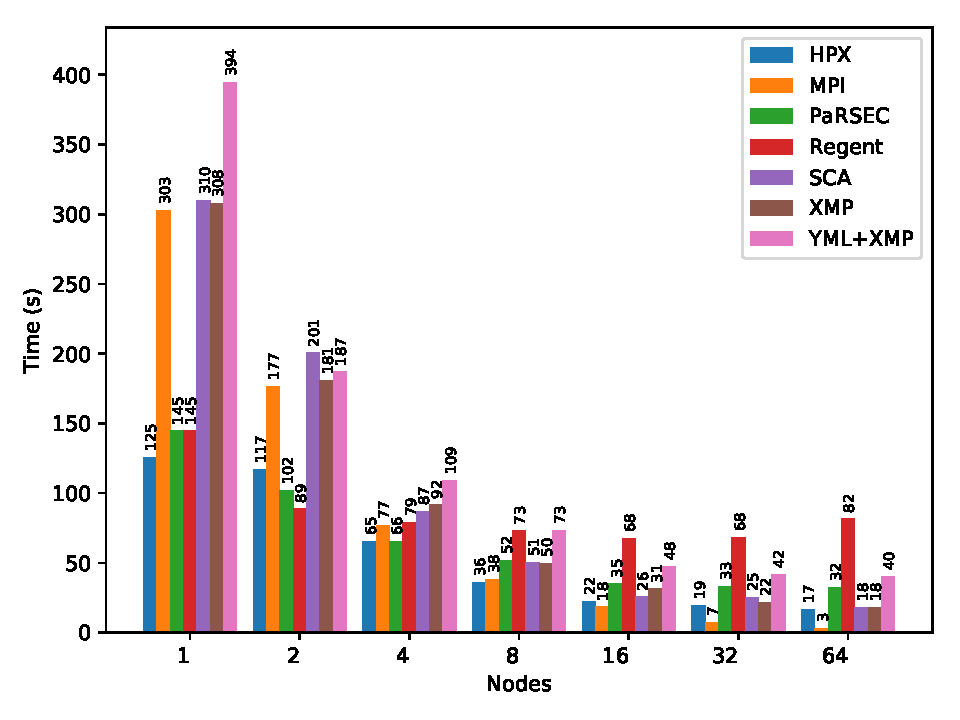
\includegraphics[width=.6\linewidth]{fig_strong_scaling_bar_task}
	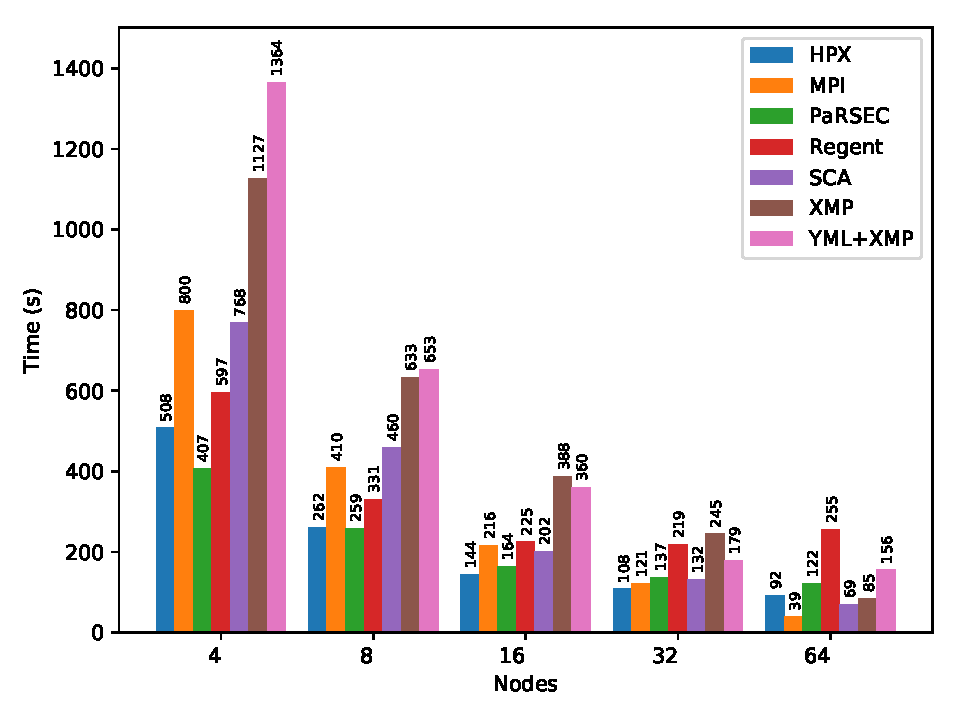
\includegraphics[width=.6\linewidth]{fig_strong_scaling_bar_task_32k}
	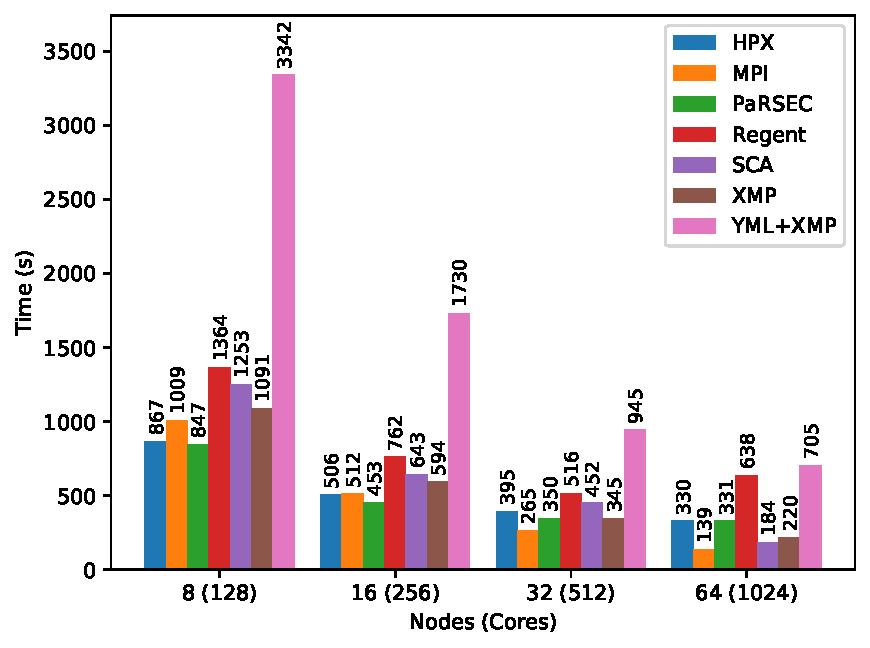
\includegraphics[width=.6\linewidth]{fig_strong_scaling_bar_task_49k}
	\caption{Execution times obtained with the block-based LU factorization implemented with several task-based programming models on a $16384 \times 16384$ matrix (top), a $32768 \times 32768$ matrix (middle) and a $49512 \times 49512$ matrix (bottom)\label{fig:perf}}
\end{figure}


Fig. \ref{fig:perf} shows the performances obtained for the LU factorization with HPX, MPI, PaRSEC, Regent, ScaLAPACK, XMP and YML+XMP on three sizes of matrices $16384 \times 16384$ (top), $32768 \times 32768$ (middle) and $49512 \times 49512$ (bottom).

On a $16384 \times 16384$ matrix, MPI is close to XMP on a small amount of nodes.
When the number of node increases, MPI becomes significantly faster than XMP.
Indeed, Fig. \ref{fig:perf} middle and bottom charts show that MPI is significantly faster than XMP for each number of node.
MPI and XMP applications share the same algorithm and a similar implementation but expressed with two different models.
This may be due to an overhead from the PGAS description and access of the data in XMP compared to MPI.

Regent, HPX and PaRSEC are relatively close to one another on a small number of cores.
However, we can outline tendencies.
PaRSEC is faster than HPX on the lower number of node then HPX becomes faster when the number of node increases.
It also seems that when the size of the matrix increases, HPX and PaRSEC performances are becoming closer and that HPX becomes faster than PaRSEC on the larger number of nodes.
Indeed, HPX becomes faster than PaRSEC after 4 nodes for a  matrix of size $16384 \times 16384$, after 16 nodes for a matrix of size $32768 \times 32768$ and after 64 nodes $49512 \times 49512$.
For the later value, the difference between the two is very small (330s vs 331) so we expect HPX to become significantly faster for this size of matrix with a greater number of nodes.

Regent is a little bit behind HPX and PaRSEC on each number of nodes and size of matrices except for 2 and 4 nodes on a $16384 \times 16384$ matrix where Regent is very efficient.
We can also notice that Regent is taking more time on 64 nodes than on 32.
This may be related to the fact that Regent does not seem to be able to manage a large number of tasks on a large number of nodes since the number of sub-matrices is decreasing when the number of cores is increasing as Table \ref{tab:blocks}, Table \ref{tab:blocks_32k} and Table \ref{tab:blocks_49k} are showing.
However, other task based languages obtain better results when the number of sub-matrices they process increase with the number of cores.
It creates more task and parallelism so that the runtime can use the resources most efficiently.

The YML+XMP applications are the slowest compared to the the applications implemented with the other models.
However, YML+XMP is the only model where tasks are also parallel and distributed.
Moreover, it also uses the file system to perform the communications between the tasks so the communications between tasks are not efficient.

Our last application uses the ScaLAPACK library to compute the LU factorization.
It performs very well on large number of nodes but HPX, PaRSEC and Regent are faster on lower number of cores for each size of matrix.
%TODO confirm
They are not using the same block based algorithm but ScaLAPACK is using a tiled algorithm that makes computations on rows and columns of the matrix \cite{ChDPW1992}.
Therefore, it is an interesting comparison to our block-based algorithms where the operations on the blocks are implemented with tasks.
For a $16384 \times 16384$ matrix ScaLAPACK and HPX are close on 64 nodes but ScaLAPACK is faster for greater size of matrices.
This may be due to the cyclic distribution of data in ScaLAPACK which induces a different communication pattern very efficient on this kind of machine and algorithm.

\subsection{Strong scaling}
\label{sec:strong_scaling}
\begin{figure}[h]
	\centering
	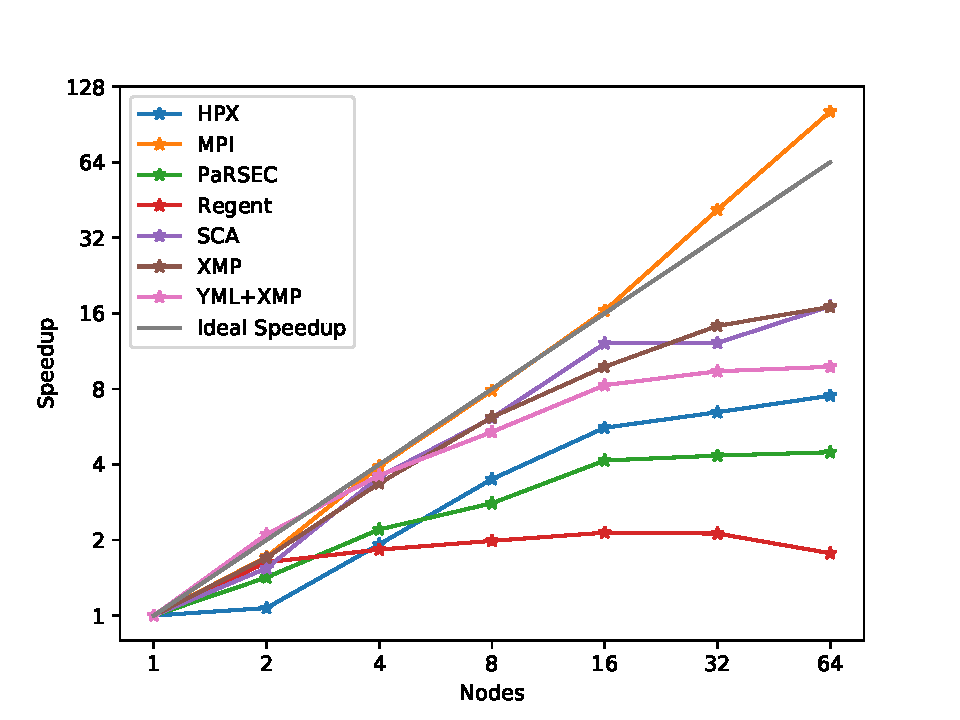
\includegraphics[width=.6\linewidth]{fig_strong_scaling_speedup_task}
	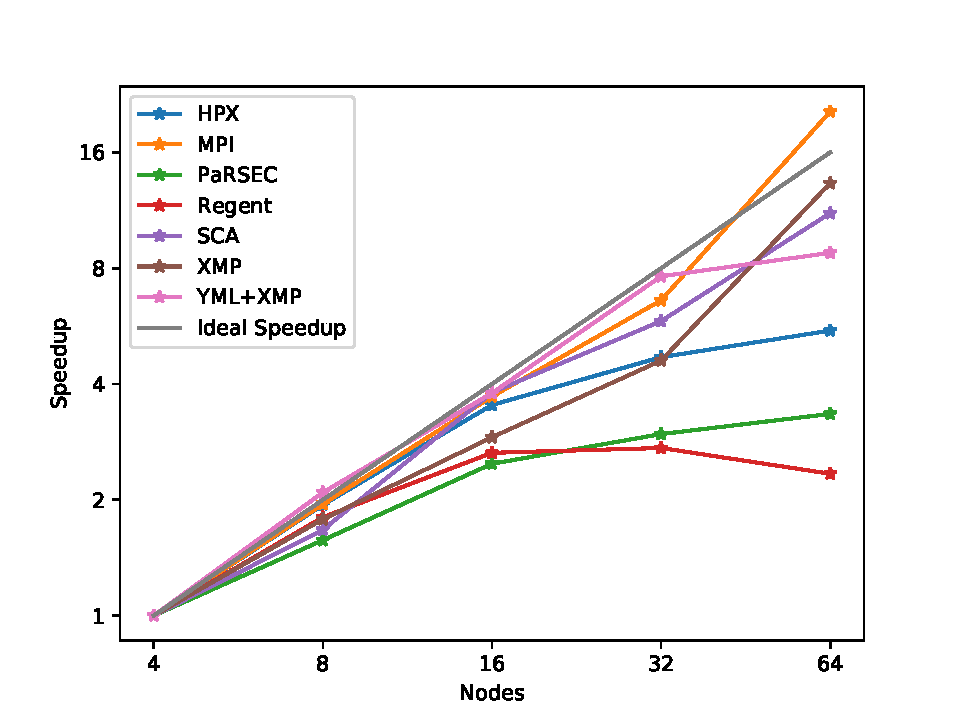
\includegraphics[width=.6\linewidth]{fig_strong_scaling_speedup_task_32k}
	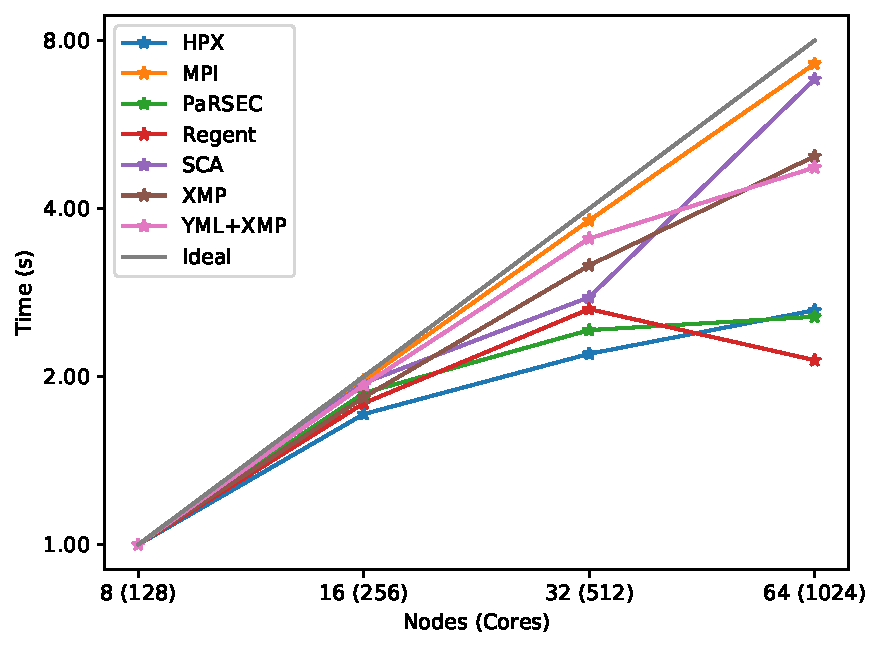
\includegraphics[width=.6\linewidth]{fig_strong_scaling_speedup_task_49k}
	\caption{Speed-ups obtained with the block-based LU factorization implemented with several task-based programming models on a $16384 \times 16384$ matrix (top), a $32768 \times 32768$ matrix (middle) and a $49512 \times 49512$ matrix (bottom) - $log_2$ scale for the y-axis\label{fig:strong_scaling}}
\end{figure}

Fig. \ref{fig:strong_scaling} shows the speed-up extracted from the performances values from Fig. \ref{fig:perf} for HPX, MPI, PaRSEC, Regent, ScaLAPACK, XMP and YML+XMP on three sizes of matrices $16384 \times 16384$ (top), $32768 \times 32768$ (middle) and $49512 \times 49512$ (bottom).
It corresponds to the ratio $t_S/t_N$ where $t_N$ is the execution time for N nodes and $t_F$ is the execution time of the first number of nodes considered in the test.
In the top chart of Fig. \ref{fig:strong_scaling}, $t_F$ is $t_1$ since the experiments start with 1 node.
In the middle (bottom) chart, $t_F$ corresponds to 4 (8).
It translates how efficiently we are managing the addition of more resources to solve the same problem.

Our MPI regular LU factorization is scaling very well as we can see on the charts.
It even exceeds the ideal speed-up with matrices of size $16384 \times 16384$ (Fig. \ref{fig:strong_scaling} top chart) and $32768 \times 32768$ (Fig. \ref{fig:strong_scaling} middle chart).
We think that it may be due to processes not having enough computations to do on 32 and 64 nodes matrices of size $16384 \times 16384$.
Indeed, when increasing the size of the matrix to $32768 \times 32768$, the strong scalability for our MPI application seems more reasonable.
The same situation occurs for 64 nodes when increasing the size of the matrix from $32768 \times 32768$ to $49512 \times 49512$.

Our task based applications obtain better scalability with the increase of the data size and the number of tasks processed by the applications.
Table \ref{tab:blocks}, Table \ref{tab:blocks_32k} and Table \ref{tab:blocks_49k} show that the number of tasks for a given number of nodes increases with the size of the matrix for each task based programming model.
It produces more parallelism and opportunities to optimize the scheduling of the tasks and improve the use of the computing resources.

Regent strong scalability decreases from 32 to 64 nodes for each size of matrix.
We expect its strong scalability to decrease even more with the increase of the number of cores.

Our HPX application is scaling better than our PaRSEC application with matrices of size $16384 \times 16384$ and $32768 \times 32768$.
It corresponds to the results we obtained in the previous section.
We can also see that PaRSEC and HPX are very close with matrices of size $49512 \times 49512$ and that HPX is exceeding PaRSEC after 32 nodes.
It seems that HPX may have a better scalability than PaRSEC on more than 64 nodes with matrices of size $49512 \times 49512$ if more nodes were available.

Finally, our YML+XMP application has the best strong scalability compared to the other task-based programming models.
Therefore, we think that this programming model will be well adapted to larger machines with a distributed system and integrated schedulers.

\subsection{Results summary}
To conclude, MPI has the best results and scalability on 64 nodes but the application does not use partial pivoting so it is not comparable to ScaLAPACK.
It is also faster than XMP since MPI routines are highly optimized.
Even though, XMP translates its directives into MPI code, the PGAS model used in XMP is not as efficient as using directly MPI.

ScaLAPACK is faster than the applications implemented with the task based programming models but it uses very efficient kernel routines to perform operations internally whereas we are using unoptimized routines.

In term of task based programming models where we implemented everything (task dependencies and tasks themselves) with the programming model, HPX is the most efficient on 64 nodes.
However, PaRSEC also shows interesting performances in specific circumstances.
Furthermore, Regent applications are not faster while increasing the number of nodes from 32 to 64.
We think that the difference of performances between those programming models comes from their ability to manage the number of tasks, the dependencies between the tasks, tasks workload and the data migrations between nodes.
Indeed, Regent performs best with a smaller amount of tasks than HPX and PaRSEC but its performances are behind them (see Table \ref{tab:blocks}, Table \ref{tab:blocks_32k} and Table \ref{tab:blocks_49k}).
HPX and PaRSEC are performing better with a higher number of smaller tasks.
They seems to distribute very efficiently the tasks on the resources and optimize the data migrations between the nodes.
Moreover, we used the default mapper for data and tasks provided by Regent and Legion.
They may not be efficient enough in our case.
Implementing a new mapper may improve the performances of our Regent application.

Finally, YML+XMP is the only programming model using tasks which are also distributed but the communications through the file system decrease its efficiency.
YML+XMP performances may not be impressive on this number of nodes but with the increase of the number of nodes and its strong scalability higher than the other task-based programming languages, YML+XMP could be able to perform better than the other programming models on a very large scale as already experienced on the K computer \cite{GuTPS2019}.
Moreover, changing the use of the file system to make the communications between the tasks to in-memory communications could improve the performances even more.


\section{Second Analysis and Selection of MPI, PaRSEC, HPX, Pegasus and YML+XMP}
	\SetKwRepeat{Struct}{struct \{}{\}}%
\newcommand{\Array}{\KwSty{Array}}
\newcommand{\Integer}{\KwSty{Integer}}

\chapter{Task-Based, Parallel and Distributed Sparse Linear Algebra Applications \label{chap:exp_sparse}}
\graphicspath{{chapters/exp_sparse/}}

The sparse matrix vector product with several matrix storage format and matrix distribution across the computing resources is the basic algorithm considered in this chapter.
Sequences of sparse matrix products are important and largely used in several applications such as iterative methods and neural network training.
However, two executions of the sparse matrix vector are enough to outline the algorithmic issues without having to perform too much computations.
Therefore, the sparse operation $A(Ax+x)$ is considered as it uses two times the sparse matrix vector product.
We implement these algorithms with the selected task based programming models and perform numerical experiments on several clusters and supercomputers.
Finally, we discuss the results obtained in the experiments.


\section{Task-Based Methods for Parallel and Distributed Algorithms}
The sparse matrix vector product is executed in a distributed and parallel environment which means that computations can be run in parallel and data may not be accessed directly since they can be stored on a different resource than where they are needed.
The data can be moved through the network but it can be costly especially in very large networks.
The goal is to implement a parallel, distributed and task based sparse matrix vector product taking advantage of this set up while getting the best execution time and reducing the communications.
In the sparse matrix vector product case, the distributed and parallel algorithms (both regular and task based) depends on the storage formats used and the distribution of the sparse matrix on the distributed resources.
There is several way of distributing the matrix : either by splitting the columns or the rows.
A combination of the two previous way of distribution, the block distribution is also considered here.
They are the main way of distributing a matrix although other ways exist like a cyclic distribution where the consecutive values are put alternatively on a distributed resource.
The sub-matrices are stored in memory with a sparse storage format.


\subsection{Data Distribution \label{sec:sla:data_distribution}}

We consider three ways of distributing the data : a distribution by rows, by columns and by blocks.
The distribution by rows and by columns are special cases of the distribution by blocks where the is only distribution across one row for the distribution by columns and where the is only distribution across one column for the distribution by rows.
The blocks are sub-matrices kept on memory with a sparse storage format.
In this section, we are considering different ways of distributing sparse matrices.
However, we are not looking into the load balancing issues that may arise if some blocks are more populated than others.


\begin{figure}[h]
	\centering
	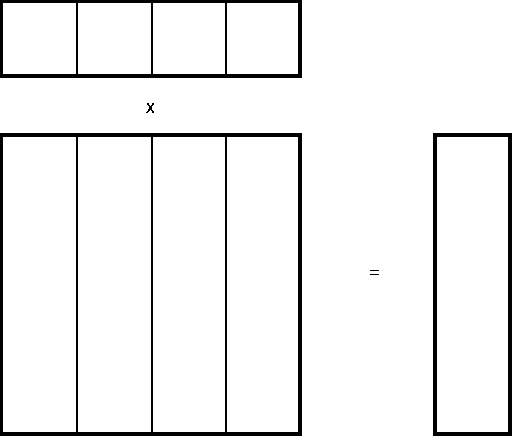
\includegraphics[width=.5\textwidth]{pmv_c}
	\caption{Distribution of the matrix by columns in which the sub-columns are compressed \label{fig:sparse:pmv_c}}
\end{figure}

The distribution by columns consists in splitting the rows and keeping the values of the same column in the same computing resource.
These columns are stored in a sparse storage format locally.
The input vector can also be split since only the rows of the vector corresponding to the columns stored in a computing resource are necessary for the matrix vector product.
The Figure \ref{fig:sparse:pmv_c} shows a matrix distributed by rows to make a matrix product vector as well as the necessary input vector and the result vector.
The result vector has the same size as the number of rows in the sub-matrices.
In this case, it corresponds to the full matrix number of rows.
However, each computing resource contains a part of the global solution of the matrix vector product.
To obtain the global result, all the distributed results have to be summed.


\begin{figure}[h]
	\centering
	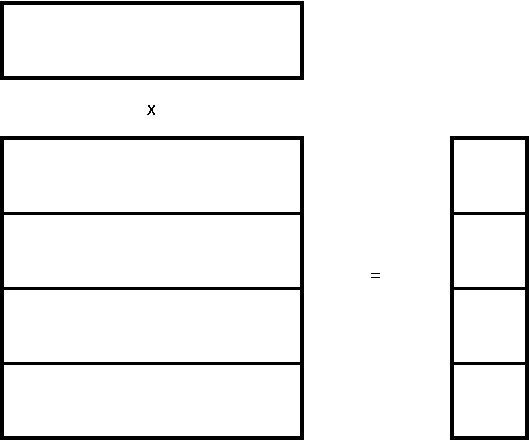
\includegraphics[width=.5\textwidth]{pmv_r}
	\caption{Distribution of the matrix by rows in which the sub-rows are compressed \label{fig:sparse:pmv_r}}
\end{figure}

The distribution by rows consists in splitting the columns and keeping the values of the same row in the same computing resource.
These rows are stored in a sparse storage format locally.
In this case, the input vector cannot be split since a complete row of the matrix may be stored in each computing resource.
In the sparse case, the rows may not be complete on each process but it can not be known in advance.
The input vector is duplicated in each computing resource.
The result vector has the same size as the number of rows in the sub-matrices.
Here, it corresponds to the number of rows in each corresponding sub-matrices.
However, each computing resource contains a sub-vector.
To obtain the global result, all the distributed results have to be gathered (which means that the global vector has just to be reconstructed without any computations).


\begin{figure}[h]
	\centering
	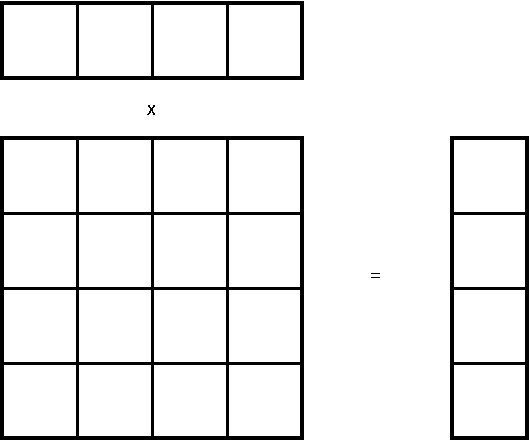
\includegraphics[width=.5\textwidth]{pmv_2D}
	\caption{Distribution of the matrix by rows and columns in which the blocks are compressed matrices \label{fig:sparse:pmv_2D}}
\end{figure}

The block distribution consists in both a distribution by rows and distribution by columns.
The matrix in split in a 2D grid way.
The $Nx \times Ny$ matrix is split in $Ngx \times Ngy$ sub-matrices.
The sub-matrices are stored in a sparse storage format locally.
In this case, the input vector is split across the columns of the matrix and the sub-vectors are duplicated on the sub-rows of the same column.
The Figure \ref{fig:sparse:pmv_r} shows a matrix distributed by blocks to perform a matrix product vector as well as the necessary input vector and the result vector with $Ngx = 4$ and $Ngy = 4$.
The result vector has the same size as the number of rows in the sub-matrices of the corresponding row.
However, each computing resource contains a part of a sub-vector.
To obtain the global result, all the distributed results of the same row have to be reduced then each rows have to be gathered if the full result vector is needed in one place.

The data distribution determines which part of the global matrix iq stored on a given computing resource.
The Section \ref{sec:sla:task_definition} points out how these data is used to perform the matrix vector product.

\subsection{Tasks Definition \label{sec:sla:task_definition}}

In this section, we consider that the matrix is divided according to one of the distribution described previously (except for the COO storage format).
Each sub-matrix is used as input of the matrix vector product tasks defined in the following algorithms.
We define data structures to store the matrices and use them in the tasks.
Finally, the algorithms for the tasks is designed.


\begin{algorithm}[h]
	\DontPrintSemicolon
	\SetAlgoVlined
	\caption{COO format data structure and matrix vector product\label{alg:sparse:spmv_coo}}
	\SetKwProg{Fn}{Task}{}{end}

	\Struct{MatrixCOO}{
		\Array{} row, col, val\;
	}
	\;
	\Fn{spmv\_coo()}{
		\KwData{m : MatrixCOO, v : Array}
		\KwResult{r : Array}
		\For{i \KwFrom 0 \KwTo m.val.size() - 1}{
			r[m.row[i]] += m.val[i] * v[m.col[i]]\;
		}
	}
\end{algorithm}

Algorithm \ref{alg:sparse:spmv_coo} defines a data structure to store the sub-matrices stored in the COO format.
It also shows the algorithm to make a matrix vector product on the sub-matrix given the proper input vector.
The data structure contains the three arrays necessary to store the matrix in the COO storage format.
In this implementation of the matrix vector product with the COO format, the sub-matrix does not have to be sorted e.g. this implementation does not expect the coordinates of the values of the matrix to be in a given range.
Therefore, this implementation can process any value in any position in any sub-matrix (which is not the case with the other storage formats).
However, we cannot deduce the range of position in the full input vector which is effectively used in the task as well as the range of position for the output vector since there is no restrictions on the range of coordinates of the values in the matrix.
Thus, this task also expect the full vector as input for the tasks (independently of the data distribution described) and output a full vector.

It can allow a better load balancing at the cost of a full vector in input and output which change how the output vector is processed to construct the full output vector.
This is discussed in Section \ref{sec:sla:task_based_parallel_algorithms}.


\begin{algorithm}[h]
	\DontPrintSemicolon
	\SetAlgoVlined
	\caption{SCOO format data structure and matrix vector product\label{alg:sparse:spmv_scoo}}
	\SetKwProg{Fn}{Task}{}{end}

	\Struct{MatrixSCOO}{
		\Array{} row, col, val\;
		\Integer{} fr, fc\;
	}
	\;
	\Fn{spmv\_scoo()}{
		\KwData{m : MatrixCOO, v : Array}
		\KwResult{r : Array}
		\For{i \KwFrom 0 \KwTo m.val.size() - 1}{
			r[m.row[i] - m.fr] += m.val[i] * v[m.col[i] - m.fc]\;
		}
	}
\end{algorithm}

Algorithm \ref{alg:sparse:spmv_scoo} defines a data structure to store the sub-matrices stored in the SCOO format in which we expect a given range of coordinates for the values contrary to the COO format.
It also shows the algorithm to make a matrix vector product on the sub-matrix given the proper input vector.
The data structure contains the three arrays necessary to store the matrix in the SCOO storage format as well as useful informations about the position of the sub-matrix in the global matrix.
These informations are the first row (\textit{fr}) and the first column (\textit{fc}) possibles in the sub-matrix (It may not correspond to the actual values stored in the sub-matrix since it corresponds to the lower boundaries of the possible coordinates in the sub-matrix for the algorithm to work properly).
The algorithm for the SCOO storage format is similar to the algorithm for COO whereas the supplementary informations are used in the algorithm to properly position the output vector.
In this case, the range of position for the input and output vectors can be computed since the range of coordinates for the values in the SCOO storage format are restricted to the data distributions discussed in Section \ref{sec:sla:data_distribution}.
Therefore, depending of the data distribution, the input and output vector shapes change.

In this case, the construction of the full output vector depends on the division of the matrix as specified in Section \ref{sec:sla:data_distribution}.
This is detailed further in Section \ref{sec:sla:task_based_parallel_algorithms}.


\begin{algorithm}[h]
	\DontPrintSemicolon
	\SetAlgoVlined
	\caption{CSR format data structure and matrix vector product\label{alg:sparse:spmv_csr}}
	\SetKwProg{Fn}{Task}{}{end}

	\Struct{MatrixCSR}{
		\Array{} idx, col, val\;
		\Integer{} fc\;
	}
	\;
	\Fn{spmv\_csr()}{
		\KwData{m : MatrixCSR, v : Array}
		\KwResult{r : Array}
		\For{i \KwFrom 0 \KwTo m.idx.size() - 1}{
			\For{j \KwFrom m.idx[i] \KwTo m.idx[i+1] - 1}{
				r[i] += m.val[j] * v[m.col[j] - m.fc]\;
			}
		}
	}
\end{algorithm}

Algorithm \ref{alg:sparse:spmv_csr} defines a data structure to store the sub-matrices stored in the CSR format in which we expect a given range of coordinates for the values.
It also shows the algorithm to make a matrix vector product on the sub-matrix given the proper input vector.
The data structure contains the three arrays necessary to store the matrix in the CSR storage format as well as useful informations about the position of the sub-matrix in the global matrix.
These informations are the first column (\textit{fc}) possibles in the sub-matrix.
As for the SCOO storage format, the ranges of position for the input and output vectors can be computed.


\begin{algorithm}[h]
	\DontPrintSemicolon
	\SetAlgoVlined
	\caption{ELL format data structure and matrix vector product\label{alg:sparse:spmv_ell}}
	\SetKwProg{Fn}{Task}{}{end}

	\Struct{MatrixELL}{
		\Array{} col, val\;
		\Integer{} fc, max\_col\;
	}
	\;
	\Fn{spmv\_ell()}{
		\KwData{m : MatrixELL, v : Array}
		\KwResult{r : Array}
		\For{i \KwFrom 0 \KwTo m.lrs - 1}{
		 	\For{j \KwFrom 0 \KwTo m.max\_col - 1}{
		 		r[i + m.rpos] += m.val[i * m.max\_col + j] * v[m.col[i * m.max\_col + j]- m.fc]\;
		 	}
		}
	}
\end{algorithm}

Algorithm \ref{alg:sparse:spmv_ell} defines a data structure to store the sub-matrices stored in the ELL format in which we expect a given range of coordinates for the values.
It also shows the algorithm to make a matrix vector product on the sub-matrix given the proper input vector.
The data structure contains the number of columns needed in the arrays and the two arrays necessary to store the matrix in the ELL storage format as well the first column (\textit{fc}) possibles in the sub-matrix which is used in this algorithm.
As for the SCOO and CSR storage formats, the ranges of position for the input and output vectors can be computed.

In this section, we presented the algorithms used to perform the matrix vector product on the sub-matrices in the tasks with the COO, SCOO, ELL and CSR sparse storage formats.
They are used to perform the matrix vector product on the global matrix.
The Section \ref{sec:sla:task_based_parallel_algorithms} introduces the task-based algorithms to perform the sparse matrix vector product and construct the complete output vector.

\subsection{Task-Based Parallel Algorithms \label{sec:sla:task_based_parallel_algorithms}}

In this section, we introduce the task-based algorithms for the high level sparse matrix vector product.
They use the tasks designed in Section \ref{sec:sla:task_definition} to perform the matrix vector product on the global matrix.
In the algorithms the \textit{SPMV} tasks corresponds to one of the \textit{spmv\_*} defined in the previous section except for \textit{spmv\_coo} which needs a different data distribution.
These high level task-based algorithms are independent of the matrix storage format.


\begin{algorithm}[h]
	\DontPrintSemicolon
	\caption{Parallel and Distributed Task Based Algorithm for the Sparse  Matrix Vector Product with Distributed Rows \label{alg:sparse:task_spmv_rows}}
	\ParFor{i \KwFrom 0 \KwTo $Ngr - 1$}{
		M[i] = GenMatrix(i, $Ngr$, $Nr$, $Nc$)\;
	}
	V = GenVector($Ngc$)\;
	\;
	\ParFor{i \KwFrom 0 \KwTo $Ngr - 1$}{
		R[i] = SPMV(M[i], V)\;
	}
	\;
	\tcc{Necessary data migrations to relocate data for a new SPMV}
	\If{dataRelocation}{
		V = MERGE(R[0 : $Ngr - 1$])\;
	}

\end{algorithm}

Algorithm \ref{alg:sparse:task_spmv_rows} performs the matrix vector product on the global matrix when it is distributed by rows as shown in Figure \ref{fig:sparse:pmv_r}.
First, we need to generate or load the initial sub-matrices and sub-vectors to use them in the tasks.
With this data distribution, each task needs the full vector and output a piece of vector.
Then, the \textit{SPMV} tasks can be run on each sub-matrix.
Finally, the output vector has to be reconstructed.
In this case, we need to combine each of the output pieces of vector and create a full vector that can be reused later on.


\begin{algorithm}[h]
	\DontPrintSemicolon
	\caption{Parallel and Distributed General Task Based Algorithm for the Sparse  Matrix Vector Product with Distributed Columns \label{alg:sparse:task_spmv_col}}
	\ParFor{j \KwFrom 0 \KwTo $Ngc - 1$}{
		M[j] = GenMatrix(j, $Ngc$, $Nr$, $Nc$)\;
		V[j] = GenVector(j, $Ngc$, $Nc$)\;
	}
	\;
	\ParFor{j \KwFrom 0 \KwTo $Ngc - 1$}{
		Rl[j] = SPMV(M[j], V[j])\;
	}
	\;
	\tcc{Necessary data migrations to relocate data for a new SPMV}
	\uIf{dataRelocation}{
%		Rg = REDUCE(Rl[0 : $Ngc - 1$])\;
%		V[0 : $Ngc - 1$] = BROADCAST(Rg)\;
		\ParFor{j \KwFrom 0 \KwTo $Ngc - 1$}{
			V[j] = SUM(Rl[0 : $Ngc - 1$])\;
		}
	}
	\Else {
		Rg = SUM(Rl[0 : $Ngc - 1$])\;
	}
\end{algorithm}

Algorithm \ref{alg:sparse:task_spmv_col} performs the matrix vector product on the global matrix when it is distributed by columns as shown in Figure \ref{fig:sparse:pmv_c}.
With this data distribution, each task needs the only the piece of vector required to make the matrix vector product and output a full vector.
Then, the \textit{SPMV} tasks can be run on each sub-matrix.
In this case, the reconstruction of the full output vector is made by summing all the vectors which are results of the \textit{SPMV} task.


\begin{algorithm}[h]
	\DontPrintSemicolon
	\caption{Parallel and Distributed Task Based Algorithm for the Sparse  Matrix Vector Product with 2D Distributed Matrices \label{alg:sparse:task_spmv_2D}}
	\ParFor{j \KwFrom 0 \KwTo $Ngc - 1$}{
		\ParFor{i \KwFrom 0 \KwTo $Ngr - 1$}{
			M[i, j] = GenMatrix(i, j, $Ngr$, $Ngc$, $Nr$, $Nc$)\;
		}
		V[j] = GenVector(j, $Ngc$, $Nc$)\;
	}
	\;
	\ParFor{i \KwFrom 0 \KwTo $Ngr - 1$}{
		\ParFor{j \KwFrom 0 \KwTo $Ngc - 1$}{
			Rl[i, j] = SPMV(M[i, j], V[j])\;
		}
	}
	\ParFor{j \KwFrom 0 \KwTo $Ngc - 1$}{
		V[j] = SUM(Rl[i, 0 : $Ngc - 1$])\;
	}
	\;
	\If{dataRelocation}{
		Vm = MERGE(R[0 : $Ngr - 1$])\;
	}
\end{algorithm}

Algorithm \ref{alg:sparse:task_spmv_2D} performs the matrix vector product on the global matrix when it is distributed as shown in Figure \ref{fig:sparse:pmv_2D}.
With the 2D data distribution, each column of sub-matrices needs the corresponding sub-part of the input vector.
Then, the \textit{SPMV} tasks can be run on each sub-matrix.
In this case, the reconstruction of the full output vector is made by summing all the vectors which are results of the \textit{SPMV} task from the same row of sub-matrices then gathering the result of the sum in a complete vector.

\begin{algorithm}[h]
	\DontPrintSemicolon
	\caption{Parallel and Distributed Task Based Algorithm for the Sparse  Matrix Vector Product with COO matrices \label{alg:sparse:task_spmv_COO}}
	\ParFor{j \KwFrom 0 \KwTo $N - 1$}{
		M[i] = GenMatrixCOO(i, $N$, $Nr$, $Nc$)\;
	}
	V = GenVector($Nc$)\;
	\;
	\ParFor{j \KwFrom 0 \KwTo $Ngc - 1$}{
		Rl[i, j] = SPMV(M[i, j], V[j])\;
	}
	\;
	V = SUM(Rl[0 : $N - 1$])\;
\end{algorithm}

Algorithm \ref{alg:sparse:task_spmv_COO} performs the matrix vector product on the global matrix when it is distributed as a non restricted and split COO sparse storage format.
The matrix is split so that there is the same amount of values in each sub-matrix.
This improves the load balancing of the computations in the tasks (each task has the same number of computations).
With this data distribution, the shape of the input and output vectors cannot be anticipated so the matrix vector product task expect the full vector as input and return a full vector.
Then, to compute the output of the global matrix vector product, the output vector of each task has to be summed.

This section introduced the data distribution considered in this study.
They are a division by blocks of rows, blocks of columns, rectangle blocks in the rows and columns and a distribution with the same number of value in each task.
We also introduced the algorithms to implement the tasks for the sub-matrices with the different sparse matrix storage formats (COO, SCOO, ELL and CSR) as well as the task-based algorithms to perform the matrix vector product on the global matrix.
These algorithms are used to implement a task-based sparse matrix vector application and compare the performances obtained across different programming models, matrix storage format and data distribution in Section \ref{sec:sla:exp}.

\section{Numerical Experiments \label{sec:sla:exp}}
In this section, a sparse matrix vector product using task based, distributed and parallel programming models as well as the numerical experiments performed.
Three classes of programming models were chosen to implement the sparse matrix vector product.
First, MPI, a message passing library was chosen since it is the main stream library used to perform communications and global operation across multiple nodes on supercomputers.
Secondly, we chose to use a fine grain task based programming model in which dependencies between tasks are data oriented.
HPX, Legion and PaRSEC are such programming models and we chose to use only HPX since they cover the same kind of properties.
Finally, the last class is a parallel and distributed task based programming model in which tasks themselves are also parallel and distributed on a subset of the resources allocated to the application.
In this case, YML+XMP was chosen over Pegasus and Swift since YML+XMP has been more used than the other two.

\subsection{Application Description}
The sparse matrix vector product and the sparse $A(Ax+x)$ has been implemented with MPI, HPX, and YML+XMP.
The sparse operation $A(Ax+x)$ is the combination of two sparse matrix vector product $Ax$ with additional sum with the $x$ vector.
Therefore, a kernel performing the sparse $Ax$ has been implemented with the different storage format and is used as the base in MPI, HPX and YML+XMP to perform the sparse matrix vector product on the sub-matrices distributed on the computing resources.
This kernel is called in the HPX and YML+XMP tasks and the MPI processes to perform the sparse matrix vector product on the local data.
Then the programming model is used to make the appropriate data migrations in order to combine and form the output vector according to the algorithms introduced in Section \ref{sec:sla:task_based_parallel_algorithms}.

The kernel is designed to perform the sparse matrix vector product on the sub-matrices obtained from the split of the global matrix.
The input matrix can be split over a 2D grid with particular cases in which there is only one column (split only across rows) or only one row (split only across columns) as introduced in Section \ref{sec:sla:data_distribution}.
The $N_r \times N_c$ matrix is divided into an $N_{gr} \times N_{gc}$ grid.
This kernel is called in the MPI processes to perform the sparse matrix vector product on the local matrices.
In MPI, $N_{gr} \times N_{gc}$ is equal to the number of avail processes in the application.
This allow each process to manage its sub-matrix.
The kernel is also called in HPX tasks to perform the sparse matrix vector product on the sub-matrix managed into a tasks.
For HPX, there is no particular restrictions on $N_{gr}$ and $N_{gc}$ since there is no obligations to execute tasks on each worker process, even though, these workers could be idling due to the lack of tasks.
Finally, the kernel is also used in YML+XMP components (tasks) to perform the sparse matrix vector product in each processes allocated to each sparse matrix vector product task.
Afterwards, the output vector is combined inside the tasks then combined at the level of the graph of tasks.
Each YML tasks have an allocated number of processes.
Therefore, in order to make sure that each process works on a sub-matrix, the number of sub-matrices ($N_{tr} \times N_{tc}$) in the grid of sub-matrices in the tasks have to match the number of processes allocated to the tasks.
In our application, each task has the same number of processes allocated, which means that, in order to fill each processes of the tasks, the number of rows (resp. columns) in the division of the global matrix has to match the number of rows (resp. columns) in the division of the matrix in the tasks multiplied by the number of rows (resp. columns) in the division of the matrix at the task level (see Figure \ref{fig:sparse:yml_matrix_div}).

\begin{figure}[h]
        \centering
		\includegraphics[width=.4\textwidth]{{{yml_matrix_div}}}
        \caption{Two level of division in matrices managed by YML+XMP \label{fig:sparse:yml_matrix_div} with $3 \times 3$ task level matrices in which there is $4 \times 4$ sub-matrices}
\end{figure}

The kernel has been implemented to support the CSR, ELL, COO, SCOO and dense storage formats.
The sparse matrix vector products for the different storage formats were implemented according to the algorithms introduced in Section \ref{sec:sla:task_definition}.
Then, for each storage format and each programming model considered, the distributed and parallel version of the sparse matrix vector has been implemented based on the algorithms described in Section \ref{sec:sla:task_based_parallel_algorithms}.

Moreover, the sparse operation $A(Ax+x)$ has also been implemented on top the sparse matrix vector product.
Therefore, it also supports the CSR, ELL, COO, SCOO and dense storage formats as well as the different matrix distribution possibilities.
This operation has been implemented in MPI, HPX and YML+XMP.
It consists in a call to the sparse matrix vector product followed by the sum of the output vector with $x$ then another sparse matrix vector product.
The communications, the building of the output vector depending on the distribution of the matrix and the sum are managed with the programming models in which the application is implemented.

Finally, separate libraries containing the kernel as well as the MPI and HPX extensions of the kernel has been created.
YML+XMP does not support the creation of libraries therefore, the sparse matrix vector product and the sparse operation $A(Ax+x)$ were directly implemented as applications.
The libraries also contain functions to generate distributed sparse matrices and the YML+XMP applications has tasks for this purpose.
The sparse matrices can be generated in each one of the supported storage format and in the data distribution introduced in Section \ref{sec:sla:data_distribution}.
These matrices are the C-diagonal Q-perturbed matrices introduced in Chapter \ref{chap:methods}.
They are were used to perform numerical experiments which is presented in the next section.


\subsection{Results and Analyses on Total Petascale Pangea II}
In these experiments, the sparse operation $A(Ax+x)$ has been performed on a sparse matrix stored COO, SCOO, ELL and CSR where $A$ is the sparse matrix and $x$ a vector.
This operation has been chosen as test due to the fact that the output vector has to be recombined after the local sparse matrix vector in order to reuse it in the next sparse matrix vector product.
The C-diagonal Q-perturbed matrices introduced in Chapter \ref{chap:methods} are used to evaluate the performances of the different programming models and storage formats.
To do so, we perform strong scaling experiments on 2 000 000 $\times$ 2 000 000 and 4 000 000 $\times$ 4 000 000 C-diagonal Q-perturbed matrices for C = 300 and several values of Q.
Moreover, we also study the impact of the number of values by rows by trying multiple values of C.
Finally, we perform weak scaling experiments with the C-diagonal Q-perturbed matrices for C=300 by increasing the number of values in the matrix depending on the number of cores used to run the application.

\subsubsection{Pangea II}
Pangea II is the supercomputer on which the experiments have been performed.
It is owned by Total and located in Pau, France.
This supercomputer is composed of nodes built with 2 Xeon E5-2680v3 12C 2.5GHz processors for a total of 220 800 cores.
The nodes are connected with Infiniband FDR interconnects.
It performs at 5.283 PFlop/s for Linpack and 162.692 TFlop/s for HPCG.

\subsubsection{Best Results Selection}
These experiments depend on several parameters.
The programming model is the first of them.
There are also the parameters related to the test matrices used, C and Q as well as the size of the matrix.
Moreover, the data distribution which can be represented by the 2D grid used to divide the matrix adds two more parameters, $N_{gr}$ and $N_{gc}$.
Finally, YML+XMP also adds several parameters to tune the two levels of parallelism it offers.
These parameters are the number of processes allocated per task, the grid used to divide the matrix in the tasks and the higher level grid used to determine which part of the matrix is used in tasks.
Even if these parameters are related, which reduces the range of values to try, there is a large amount of possibilities to try.

Therefore, after running the applications, despite using only a subset of the possible cases to try, a large number of runs for the different parameters is produced.
Then, we have to select the case that produces the best execution time depending on which case we want to display.
For instance, if we want the best case for MPI for a given matrix size, storage format, C, Q and a 2 nodes, the results change depending on the data distribution.
Thus, we have to select which data distribution has made the best performances.
The application is run multiple time for a given data distribution so we take the median execution time as metric to compare the different data distributions.
Then, we chose the case that has the best median (usually the smallest since we want the fastest execution time).

\subsubsection{Strong scaling with a 2 000 000 $\times$ 2 000 000 sparse matrix}
Strong scaling experiments on the operation $A(Ax+x)$ have been performed with a 2 000 000 $\times$ 2 000 000 sparse C-diagonal Q-perturbed matrices for C = 300 and several values of Q.
The matrix was stored in 4 storage formats : CSR, COO, SCOO and ELL.
The applications were implemented in MPI, HPX and YML+XMP.
We use a dense vector with fixed values that is generated during the execution of the applications.

\begin{figure}[h]
        \centering
        \includegraphics[width=.45\textwidth]{{{fig_pangea2_nr2000000_lHPX_fCSR}}}
        \includegraphics[width=.45\textwidth]{{{fig_pangea2_nr2000000_lHPX_fELL}}}
        \includegraphics[width=.45\textwidth]{{{fig_pangea2_nr2000000_lHPX_fCOO}}}
        \includegraphics[width=.45\textwidth]{{{fig_pangea2_nr2000000_lHPX_fSCOO}}}

        \caption{Strong scaling considering HPX and several storage formats for a 2 000 000 $\times$ 2 000 000 matrix with C = 300 on Pangea II. Legend is (model, format, Q). \label{fig:sla:pangea2_nr2000000_lHPX}}
\end{figure}

Figure \ref{fig:sla:pangea2_nr2000000_lHPX} summarizes the results obtained from the experiments with HPX in which the operation $A(Ax+x)$ is applied on a 2 000 000 $\times$ 2 000 000 sparse C-diagonal Q-perturbed matrices for C = 300 and a vector.
This figure shows the execution time for the different sparse storage formats depending on the number of nodes (cores).
For CSR, ELL and SCOO, HPX has a very good strong scalability up to 4 nodes then the performance improvement gained from the increase in computing resources diminishes.
ELL and CSR have close performances on small number of nodes and CSR is better when the number of nodes increases.
They perform better than the COO and SCOO.
COO is the slowest within the HPX implementations.
This format is a bit different since the values of the matrix are not restricted to a 2D grid like the others.
Therefore, the output of each local sparse matrix vector product has to be summed to generate the complete output and this vector has the size of the rows of the full matrix since we do not restrict the positions of the values in the sub-matrices of this format.
Furthermore, this sum is a very costly reduction since it concerns all the sub-matrices and the reduced vector is very large.

% todo update with results
The best data distribution for SCOO, CSR and ELL is 3, 4 or 6 sub-columns until 8 nodes and it starts to increase to 8 or 12 for 16 nodes.
For COO, there is no data distribution according to row or columns since it is divided according to a number of division.
In practice, the COO are divided in $N_{gr} \times N_{gc}$ where $N_{gr} \times N_{gc}$ is the grid in which the other storage format divide their matrix.
The best data distribution is similar for SCOO, CSR and ELL since they use the same pattern to combine the output vector.


\begin{figure}[h]
        \centering
        \includegraphics[width=.45\textwidth]{{{fig_pangea2_nr2000000_lMPI_fCSR}}}
        \includegraphics[width=.45\textwidth]{{{fig_pangea2_nr2000000_lMPI_fELL}}}
        \includegraphics[width=.45\textwidth]{{{fig_pangea2_nr2000000_lMPI_fCOO}}}
        \includegraphics[width=.45\textwidth]{{{fig_pangea2_nr2000000_lMPI_fSCOO}}}

        \caption{Strong scaling considering MPI and several storage formats for a 2 000 000 $\times$ 2 000 000 matrix with C = 300 on Pangea II. Legend is (model, format, Q). \label{fig:sla:pangea2_nr2000000_lMPI}}
\end{figure}

Figure \ref{fig:sla:pangea2_nr2000000_lMPI} summarizes the results obtained from the experiments with MPI in which the operation $A(Ax+x)$ is applied on a 2 000 000 $\times$ 2 000 000 sparse C-diagonal Q-perturbed matrices for C = 300 and a vector.
This figure shows the execution time for the different sparse storage formats depending on the number of nodes (cores).
CSR obtains the vest performances with MPI.
CSR and ELL have very close performances for Q = 0 and, for the other values of Q, it is SCOO who is very close to CSR.
CSR and SCOO perform better than ELL and COO.
COO is the slowest due to the fact that the output of each sub-matrix has to be summed and the output vector is of the size the global number of rows of the matrix.
However it is very close to ELL when Q > 0 despite its costly global reduction.

% todo update with results
The best data distribution for SCOO and CSR is 1 sub-row until 8 nodes.
Then, starting at 16 nodes, there is cases in which the best performances are with 1 sub-column.
For ELL, the best data distribution is with 1 sub-column except for 8 nodes where it is 4 sub-columns sometimes.
As with HPX, for COO, there is no data distribution according to row or columns.
It is interesting to notice that, SCOO and CSR obtain the best performances with the same data distribution and ELL best performances are obtained with another data distribution with MPI.


\begin{figure}[h]
        \centering
        \includegraphics[width=.45\textwidth]{{{fig_pangea2_nr2000000_lYML_fCSR}}}
        \includegraphics[width=.45\textwidth]{{{fig_pangea2_nr2000000_lYML_fELL}}}
        \includegraphics[width=.45\textwidth]{{{fig_pangea2_nr2000000_lYML_fCOO}}}
        \includegraphics[width=.45\textwidth]{{{fig_pangea2_nr2000000_lYML_fSCOO}}}

        \caption{Strong scaling considering YML and several storage formats for a 2 000 000 $\times$ 2 000 000 matrix with C = 300 on Pangea II. Legend is (model, format, Q).  \label{fig:sla:pangea2_nr2000000_lYML}}
\end{figure}

Figure \ref{fig:sla:pangea2_nr2000000_lYML} summarizes the results obtained from the experiments with YML in which the operation $A(Ax+x)$ is applied on a 2 000 000 $\times$ 2 000 000 sparse C-diagonal Q-perturbed matrices for C = 300 and a vector.
This figure shows the execution time for the different sparse storage formats depending on the number of nodes (cores).
% todo update with results
In COO and SCOO, the performances are quite stable and we obtain execution time close for the different values of Q.
Until 4 nodes, there is a slight improvement of performances  for COO and SCOO execution times stay almost constant.
Then, for the increase from 4 nodes to 8 nodes, the performances plummet dramatically.
We think it is due to the increasing number of processes making IOs (96 to 192) to communicate the data between the tasks since YML uses the file system to pass data.
This induces a great variability between the results.
On the other hand, CSR and ELL performances have more variability and it is difficult to find a logical pattern.
CSR seems to have better performances overall but there is some cases where the other storage formats are prevalent.

Furthermore, YML+XMP introduces more parameters to describe the data distribution in the tasks and across the different tasks.
This is an open set of parameters as the matrix can be divided into any shape.
Even though there is relation between the parameters, it is still a large amount of parameters to try out.
Moreover, due to technical issues, multiple YML+XMP applications cannot be run at same time while it is perfectly possible to run several MPI or HPX applications at the same time.
This greatly limit the range of parameters that can be tested since it is not possible to take advantage of the large amount of computing resources available.
The constraint to run only one application at a time and having a lot more parameters to try with YML+XMP lets the possibility of the existence of parameters that could produce better performances than the ones used in the current experiments.
We tried as much parameters we believed would lead to interesting results as we could.

%\begin{figure}[h]
%        \centering
%        \includegraphics[width=.45\textwidth]{{{fig_pangea2_nr2000000_lYML1x1_fCSR}}}
%        \includegraphics[width=.45\textwidth]{{{fig_pangea2_nr2000000_lYML1x1_fELL}}}
%        \includegraphics[width=.45\textwidth]{{{fig_pangea2_nr2000000_lYML1x1_fCOO}}}
%        \includegraphics[width=.45\textwidth]{{{fig_pangea2_nr2000000_lYML1x1_fSCOO}}}
%
%        \caption{Strong scaling considering YML with the matrix in only one block and several storage format for a 2 000 000 $\times$ 2 000 000 matrix with C = 300 on Pangea II. Legend is (model, format, Q). \label{fig:sla:pangea2_nr2000000_lYML1x1}}
%\end{figure}
%Figure \ref{fig:sla:pangea2_nr2000000_lYML1x1}
%\begin{table}[h]
%	\begin{tabular}{cccccccccccc}
\hline
Cases & Nodes& BGC& BGR& CPT& GC& GR& LGC& LGR& median & N & Ncase \\
\hline
\multirow{4}{*}{('YML', 'CSR', 0.0)}& 1& 1& 2& 24& 2& 24& 2& 12& 3.4773& 3& 16\\
& 2& 1& 2& 24& 24& 2& 24& 1& 3.0802& 5& 14\\
& 4& 2& 2& 48& 6& 32& 3& 16& 5.5149& 1& 20\\
& 8& 1& 2& 192& 1& 384& 1& 192& 5.4662& 5& 19\\
\hline
\multirow{4}{*}{('YML', 'CSR', 0.2)}& 1& 1& 2& 24& 1& 48& 1& 24& 3.1105& 3& 16\\
& 2& 2& 1& 48& 48& 2& 24& 2& 3.2017& 2& 14\\
& 4& 2& 2& 48& 6& 32& 3& 16& 5.593& 1& 20\\
& 8& 1& 2& 192& 1& 384& 1& 192& 5.7279& 5& 19\\
\hline
\multirow{4}{*}{('YML', 'CSR', 0.4)}& 1& 1& 2& 24& 2& 24& 2& 12& 3.2923& 3& 16\\
& 2& 1& 2& 24& 24& 2& 24& 1& 2.8888& 5& 14\\
& 4& 2& 1& 48& 96& 1& 48& 1& 3.5201& 2& 20\\
& 8& 1& 2& 192& 12& 32& 12& 16& 4.315& 3& 17\\
\hline
\multirow{4}{*}{('YML', 'CSR', 0.6)}& 1& 1& 2& 24& 2& 24& 2& 12& 3.3289& 3& 16\\
& 2& 1& 2& 24& 24& 2& 24& 1& 3.1826& 5& 14\\
& 4& 2& 1& 48& 96& 1& 48& 1& 3.9313& 2& 20\\
& 8& 1& 2& 192& 12& 32& 12& 16& 4.2311& 3& 17\\
\hline
\multirow{4}{*}{('YML', 'CSR', 0.8)}& 1& 1& 2& 24& 1& 48& 1& 24& 3.1635& 3& 16\\
& 2& 2& 1& 48& 48& 2& 24& 2& 3.0951& 2& 14\\
& 4& 2& 1& 48& 96& 1& 48& 1& 3.4505& 2& 20\\
& 8& 1& 2& 192& 12& 32& 12& 16& 4.1401& 3& 17\\
\hline
\multirow{4}{*}{('YML', 'CSR', 1.0)}& 1& 1& 2& 24& 2& 24& 2& 12& 3.0996& 3& 16\\
& 2& 2& 1& 48& 48& 2& 24& 2& 3.5524& 2& 14\\
& 4& 2& 1& 48& 96& 1& 48& 1& 4.1899& 2& 20\\
& 8& 1& 2& 192& 12& 32& 12& 16& 4.4705& 3& 18\\
\hline
\end{tabular}

%\end{table}
%\begin{table}[h]
%	\begin{tabular}{cccccccccccc}
\hline
Cases & Nodes& BGC& BGR& CPT& GC& GR& LGC& LGR& median & N & Ncase \\
\hline
\multirow{4}{*}{('YML', 'ELL', 0.0)}& 1& 1& 2& 24& 4& 12& 4& 6& 3.6421& 1& 10\\
& 2& 2& 1& 48& 4& 24& 2& 24& 4.0547& 3& 4\\
& 4& 2& 1& 48& 2& 48& 1& 48& 3.942& 7& 5\\
& 8& 1& 2& 192& 1& 384& 1& 192& 5.0715& 3& 6\\
\hline
\multirow{4}{*}{('YML', 'ELL', 0.2)}& 1& 1& 2& 24& 3& 16& 3& 8& 3.7532& 3& 10\\
& 2& 2& 1& 48& 4& 24& 2& 24& 6.6783& 2& 4\\
& 4& 2& 1& 48& 2& 48& 1& 48& 3.9821& 5& 5\\
& 8& 1& 2& 192& 1& 384& 1& 192& 7.1898& 3& 6\\
\hline
\multirow{4}{*}{('YML', 'ELL', 0.4)}& 1& 1& 2& 24& 3& 16& 3& 8& 3.924& 3& 10\\
& 2& 2& 1& 48& 4& 24& 2& 24& 4.3442& 3& 4\\
& 4& 2& 1& 48& 2& 48& 1& 48& 3.4307& 5& 5\\
& 8& 1& 2& 192& 1& 384& 1& 192& 6.7696& 3& 6\\
\hline
\multirow{4}{*}{('YML', 'ELL', 0.6)}& 1& 1& 2& 24& 2& 24& 2& 12& 3.7269& 3& 10\\
& 2& 2& 1& 48& 4& 24& 2& 24& 4.5151& 3& 4\\
& 4& 2& 1& 48& 2& 48& 1& 48& 4.1574& 5& 5\\
& 8& 1& 2& 192& 1& 384& 1& 192& 6.1698& 3& 6\\
\hline
\multirow{4}{*}{('YML', 'ELL', 0.8)}& 1& 1& 2& 24& 1& 48& 1& 24& 3.6055& 3& 9\\
& 2& 2& 1& 48& 4& 24& 2& 24& 5.4453& 3& 4\\
& 4& 2& 1& 48& 2& 48& 1& 48& 3.8436& 5& 5\\
& 8& 4& 1& 48& 16& 12& 4& 12& 9.3383& 1& 6\\
\hline
\multirow{4}{*}{('YML', 'ELL', 1.0)}& 1& 1& 2& 24& 2& 24& 2& 12& 4.002& 3& 9\\
& 2& 2& 1& 48& 4& 24& 2& 24& 4.1681& 3& 4\\
& 4& 2& 1& 48& 2& 48& 1& 48& 4.1922& 5& 5\\
& 8& 1& 2& 192& 1& 384& 1& 192& 6.8561& 3& 6\\
\hline
\end{tabular}


%python create_figure.py pangea2_tbsla_YML1x1.json -f op:a_axpx -f success:true -f matrixtype:cqmat -f machine:Pangea2 -l lang:YML -l format:ELL -l Q -l NR:2000000 -l C:300 -s GR -s GC -s LGR -s LGC -s BGR -s BGC -s CPT -coi nodes -voi time_op -o /Users/administrateur/Desktop/work/Thesis/phd_dissertation/chapters/exp_sparse/fig_pangea2_nr2000000_lYML_fELL.pdf -xlabel "Nodes (Cores)" -ylabel "Time (s)" -cpn 24


%\end{table}
%\begin{table}[h]
%	\begin{tabular}{cccccccccccc}
\hline
Cases & Nodes& BGC& BGR& CPT& GC& GR& LGC& LGR& median & N & Ncase \\
\hline
\multirow{4}{*}{('YML', 'COO', 0.0)}& 1& 1& 2& 24& 3& 16& 3& 8& 3.9307& 1& 16\\
& 2& 1& 2& 48& 2& 48& 2& 24& 3.5267& 1& 14\\
& 4& 2& 1& 48& 24& 4& 12& 4& 3.1323& 3& 16\\
& 8& 1& 2& 96& 2& 96& 2& 48& 5.394& 3& 14\\
\hline
\multirow{4}{*}{('YML', 'COO', 0.2)}& 1& 1& 2& 24& 6& 8& 6& 4& 3.849& 1& 16\\
& 2& 1& 2& 48& 2& 48& 2& 24& 3.0919& 1& 14\\
& 4& 2& 1& 48& 24& 4& 12& 4& 2.9645& 3& 17\\
& 8& 1& 2& 96& 2& 96& 2& 48& 6.3038& 3& 13\\
\hline
\multirow{4}{*}{('YML', 'COO', 0.4)}& 1& 1& 2& 24& 6& 8& 6& 4& 3.7139& 1& 15\\
& 2& 1& 2& 24& 24& 2& 24& 1& 3.1377& 3& 14\\
& 4& 1& 2& 96& 6& 32& 6& 16& 3.0372& 1& 17\\
& 8& 1& 2& 96& 1& 192& 1& 96& 5.9068& 3& 14\\
\hline
\multirow{4}{*}{('YML', 'COO', 0.6)}& 1& 1& 2& 24& 6& 8& 6& 4& 3.9468& 1& 15\\
& 2& 1& 2& 48& 2& 48& 2& 24& 3.2917& 1& 14\\
& 4& 2& 1& 48& 24& 4& 12& 4& 3.1861& 3& 17\\
& 8& 1& 2& 96& 1& 192& 1& 96& 5.6193& 3& 14\\
\hline
\multirow{4}{*}{('YML', 'COO', 0.8)}& 1& 1& 2& 24& 3& 16& 3& 8& 3.8611& 1& 15\\
& 2& 1& 2& 24& 24& 2& 24& 1& 3.1965& 3& 14\\
& 4& 2& 1& 48& 24& 4& 12& 4& 3.2131& 3& 17\\
& 8& 4& 1& 48& 12& 16& 3& 16& 6.9458& 2& 15\\
\hline
\multirow{4}{*}{('YML', 'COO', 1.0)}& 1& 1& 2& 24& 1& 48& 1& 24& 3.7985& 1& 16\\
& 2& 1& 2& 48& 2& 48& 2& 24& 3.4788& 1& 14\\
& 4& 2& 1& 48& 6& 16& 3& 16& 2.9228& 3& 17\\
& 8& 1& 2& 96& 1& 192& 1& 96& 6.4428& 3& 15\\
\hline
\end{tabular}


%python create_figure.py pangea2_tbsla_YML1x1.json -f op:a_axpx -f success:true -f matrixtype:cqmat -f machine:Pangea2 -l lang:YML -l format:COO -l Q -l NR:2000000 -l C:300 -s GR -s GC -s LGR -s LGC -s BGR -s BGC -s CPT -coi nodes -voi time_op -o /Users/administrateur/Desktop/work/Thesis/phd_dissertation/chapters/exp_sparse/fig_pangea2_nr2000000_lYML_fCOO.pdf -xlabel "Nodes (Cores)" -ylabel "Time (s)" -cpn 24


%\end{table}
%\begin{table}[h]
%	\begin{tabular}{cccccccccccc}
\hline
Cases & Nodes& BGC& BGR& CPT& GC& GR& LGC& LGR& median & N & Ncase \\
\hline
\multirow{5}{*}{('YML', 'SCOO', 0.0)}& 1& 1& 2& 24& 1& 48& 1& 24& 3.9036& 3& 16\\
& 2& 1& 2& 48& 2& 48& 2& 24& 3.4013& 1& 16\\
& 4& 2& 1& 48& 96& 1& 48& 1& 2.8016& 3& 17\\
& 8& 4& 1& 48& 12& 16& 3& 16& 8.7345& 2& 20\\
& 16& None& None& None& None& None& None& None& None& 0& 0\\
\hline
\multirow{5}{*}{('YML', 'SCOO', 0.2)}& 1& 1& 2& 24& 1& 48& 1& 24& 4.0968& 3& 16\\
& 2& 2& 1& 48& 4& 24& 2& 24& 3.2149& 1& 16\\
& 4& 2& 1& 48& 96& 1& 48& 1& 3.6747& 3& 18\\
& 8& 4& 1& 48& 12& 16& 3& 16& 8.1702& 2& 19\\
& 16& None& None& None& None& None& None& None& None& 0& 0\\
\hline
\multirow{5}{*}{('YML', 'SCOO', 0.4)}& 1& 1& 2& 24& 1& 48& 1& 24& 3.815& 3& 16\\
& 2& 1& 2& 24& 24& 2& 24& 1& 3.0734& 3& 16\\
& 4& 2& 1& 48& 96& 1& 48& 1& 3.4709& 3& 18\\
& 8& 4& 1& 48& 12& 16& 3& 16& 8.5992& 2& 20\\
& 16& None& None& None& None& None& None& None& None& 0& 0\\
\hline
\multirow{5}{*}{('YML', 'SCOO', 0.6)}& 1& 2& 1& 24& 48& 1& 24& 1& 3.7989& 1& 16\\
& 2& 1& 2& 48& 24& 4& 24& 2& 3.2484& 1& 17\\
& 4& 2& 1& 48& 96& 1& 48& 1& 3.5548& 3& 17\\
& 8& 4& 2& 48& 16& 24& 4& 12& 9.293& 1& 18\\
& 16& None& None& None& None& None& None& None& None& 0& 0\\
\hline
\multirow{5}{*}{('YML', 'SCOO', 0.8)}& 1& 1& 2& 24& 1& 48& 1& 24& 3.7747& 3& 16\\
& 2& 2& 1& 48& 48& 2& 24& 2& 3.2922& 1& 17\\
& 4& 2& 1& 48& 96& 1& 48& 1& 3.6671& 3& 17\\
& 8& 4& 1& 48& 16& 12& 4& 12& 8.5238& 1& 20\\
& 16& None& None& None& None& None& None& None& None& 0& 0\\
\hline
\multirow{5}{*}{('YML', 'SCOO', 1.0)}& 1& 1& 2& 24& 1& 48& 1& 24& 3.7833& 3& 16\\
& 2& 2& 1& 48& 48& 2& 24& 2& 3.2836& 1& 17\\
& 4& 2& 1& 48& 96& 1& 48& 1& 3.4435& 3& 18\\
& 8& 4& 1& 48& 16& 12& 4& 12& 8.7987& 1& 20\\
& 16& None& None& None& None& None& None& None& None& 0& 0\\
\hline
\end{tabular}


%python create_figure.py pangea2_tbsla_YML1x1.json -f op:a_axpx -f success:true -f matrixtype:cqmat -f machine:Pangea2 -l lang:YML -l format:SCOO -l Q -l NR:2000000 -l C:300 -s GR -s GC -s LGR -s LGC -s BGR -s BGC -s CPT -coi nodes -voi time_op -o /Users/administrateur/Desktop/work/Thesis/phd_dissertation/chapters/exp_sparse/fig_pangea2_nr2000000_lYML_fSCOO.pdf -xlabel "Nodes (Cores)" -ylabel "Time (s)" -cpn 24


%\end{table}
%
%\begin{table}[h]
%	\input{chapters/exp_sparse/fig_pangea2_nr2000000_lYML1x1_fCSR.tex}
%\end{table}
%\begin{table}[h]
%	\input{chapters/exp_sparse/fig_pangea2_nr2000000_lYML1x1_fELL.tex}
%\end{table}
%\begin{table}[h]
%	\input{chapters/exp_sparse/fig_pangea2_nr2000000_lYML1x1_fCOO.tex}
%\end{table}
%\begin{table}[h]
%	\input{chapters/exp_sparse/fig_pangea2_nr2000000_lYML1x1_fSCOO.tex}
%\end{table}


In these strong scaling experiments, we executed the sparse operation $A(Ax+x)$ on a 2 000 000 $\times$ 2 000 000 sparse C-diagonal Q-perturbed matrices for C = 300 and a vector while increasing the number of nodes (cores) on which we ran the applications.
We used several values for Q which represents the probability to increase the dispersion of the values in the matrix.
The applications were also implemented with three programming models : MPI, HPX and YML+XMP.
For MPI and HPX, CSR is the storage format that obtains the best performances.
It also obtains good performances with YML+XMP but it is less clear due to the variability induced by the file system.
In HPX, we see that SCOO, ELL and CSR have the same performance pattern (the curves are very similar) while the use of the different storage format explain the difference of performances between the storage formats.
SCOO has a different communication pattern that needs to reduce the output of all the matrix vector products performed in the tasks.
This reduction has been implemented for this application in HPX and is not very efficient whereas MPI reduction is heavily optimized and uses heuristics to perform a very efficient reduction.
This is why there is no difference between ELL, SCOO and CSR on one side and COO on the other side with MPI since, in MPI, all the storage format have the same performance pattern.
Finally, in YML+XMP the performances heavily rely on the capabilities of the file system due to the fact that the data going from one task to another are written then read from files.
This appears when the application is executed on 8 nodes and the number of cores used increases from 96 to 192.
Indeed, at this point, the application is taking a few more times to run on 8 nodes than to run on 4 nodes.
Current file systems are not adapted to this kind of heavy use during the execution of an application and IOs duration varies with the number of IOs operations.
Due to this, there is a lot of variability between the results.
With the parameters tried in these experiments with YML+XMP, there is no clear data distribution that stands out and performs better than the others.
CSR is leading in most of the case but the other storage formats also have cases where they perform better than CSR.

Q is also an interesting parameter that influences the performances.
It is less noticeable on YML+XMP due to the complexity of the execution model and the variability of the interactions with the file system.
However, its influences is clear for MPI and HPX since, most of the cases, the execution time is lower when Q is lower and it is higher when Q is higher.
Moreover, each application uses the same kernel to execute the sparse matrix vector product on their smallest sub-matrices.
Therefore, the differences in performances between the programming models is due to the management of the data and the implementation of the reduction to combine the output results of the sparse matrix vector product.
As such, the influence of Q is the clearest for MPI since their communications are very efficient.
For HPX and YML, the influence of Q is absorbed by our implementation of the reduction in HPX and YML+XMP as well as the IOs for YML+XMP.
In C-diagonal Q-perturbed matrices, C represents the number of values per row above the diagonal and Q is the probability to perturb the fact that all the values are packed above the diagonal.
When Q increases, the values on the row is more dispersed on this row instead of being grouped above the diagonal.
Hence, the data access pattern of the input vector changes with the different values of Q.
When Q is zero, C consecutive values starting from the diagonal of the matrix are multiplied with the input vector.
Since the values are consecutive in memory and in term of columns that are accessed in the input vector, it only accesses a portion of size C of the input vector.
This access is very regular and efficient.
However, when Q increases, the values are more dispersed in the row and the accesses to the input vector when making the multiplication is not as regular and changes from one row to another.
This random access to the memory containing the input vector is less efficient.
Therefore, Q influences the execution time of the sparse matrix vector kernel and explains the difference of performances with the different values of Q.

Then, the size of the sparse matrix is increased.
The effect of the size of the matrix is addressed in the next section.

\subsubsection{Strong scaling with a 4 000 000 $\times$ 4 000 000 sparse matrix}
We continue our strong scaling experiments on the operation $A(Ax+x)$ with a 4 000 000 $\times$ 4 000 000 sparse C-diagonal Q-perturbed matrices for C = 300 and several values of Q.
The CSR, COO, SCOO and ELL storage formats are used to in the experiments and the applications are implemented in MPI, HPX and YML+XMP.

\begin{figure}[H]
        \centering
        \includegraphics[width=.45\textwidth]{{{fig_pangea2_nr4000000_lHPX_fCSR}}}
        \includegraphics[width=.45\textwidth]{{{fig_pangea2_nr4000000_lHPX_fELL}}}
        \includegraphics[width=.45\textwidth]{{{fig_pangea2_nr4000000_lHPX_fCOO}}}
        \includegraphics[width=.45\textwidth]{{{fig_pangea2_nr4000000_lHPX_fSCOO}}}

        \caption{Strong scaling considering HPX and several storage formats for a 4 000 000 $\times$ 4 000 000 matrix with C = 300 on Pangea II. Legend is (model, format, Q). \label{fig:sla:pangea2_nr4000000_lHPX}}
\end{figure}

Figure \ref{fig:sla:pangea2_nr4000000_lHPX} summarizes the results obtained from the experiments with HPX in which the operation $A(Ax+x)$ is applied on a 4 000 000 $\times$ 4 000 000 sparse C-diagonal Q-perturbed matrices for C = 300 and a vector.
This figure shows the execution time for the different sparse storage formats depending on the number of nodes (cores).
For CSR, ELL and SCOO, HPX has a very good strong scalability up to 8 nodes then the performance improvement gained from the increase in computing resources diminishes.
ELL and CSR have close performances for 1 node and Q equal to 0.2, 0.4 and 0.6.
ELL has better performances than the other sparse storage formats for 1 node and Q = 0.
Except for the case where ELL is better, CSR leads the performances.
They perform better than the COO and SCOO.
COO is the slowest within the HPX implementations due to its costly reduction.
It is even more evident as the size of the reduced vector increases.

% todo update with results
The best data distribution for SCOO, CSR and ELL is 3, 4 or 6 sub-columns until 8 nodes and it starts to increase to 8 or 12 for 16 nodes.
This is the same parameters as the ones for the 2 000 000 $\times$ 2 000 000 matrix.
Similarly, SCOO, CSR and ELL have the same kind of performance patterns and COO does not scale at all.


\begin{figure}[H]
        \centering
        \includegraphics[width=.45\textwidth]{{{fig_pangea2_nr4000000_lMPI_fCSR}}}
        \includegraphics[width=.45\textwidth]{{{fig_pangea2_nr4000000_lMPI_fELL}}}
        \includegraphics[width=.45\textwidth]{{{fig_pangea2_nr4000000_lMPI_fCOO}}}
        \includegraphics[width=.45\textwidth]{{{fig_pangea2_nr4000000_lMPI_fSCOO}}}

        \caption{Strong scaling considering MPI and several storage formats for a 4 000 000 $\times$ 4 000 000 matrix with C = 300 on Pangea II. Legend is (model, format, Q). \label{fig:sla:pangea2_nr4000000_lMPI}}
\end{figure}

Figure \ref{fig:sla:pangea2_nr4000000_lMPI} summarizes the results obtained from the experiments with MPI in which the operation $A(Ax+x)$ is applied on a 4 000 000 $\times$ 4 000 000 sparse C-diagonal Q-perturbed matrices for C = 300 and a vector.
This figure shows the execution time for the different sparse storage formats depending on the number of nodes (cores).

ELL with Q = 0 has very good performances compared to its performances with other values of Q.
The impact of the variation of Q is greater on ELL than on the other storage formats as we can see on this figure and on the figure for the 2 000 000 $\times$ 2 000 000 matrices.
ELL also seems to have troubles scaling from 8 nodes to 16 nodes.
With these bigger matrices, CSR is still the storage format that obtains the best performances.
COO is, whithout surprises, the slowest due to the reduction on the vector of the size of the matrix.
SCOO has performances close to CSR but is still a bit behind.

% todo update with results
The best data distribution for SCOO and CSR is 1 sub-row except for Q = 0 where it is 1 sub-column.
For ELL, the best data distribution is with 1 sub-column until 8 nodes.
Then, starting from 16 nodes, it is 3 sub-columns.
As with HPX, for COO, there is no data distribution according to row or columns.
The best data distribution are similar to the ones obtained with a smaller matrix, even tough, the best data distribution is more evident with this size of matrix.

\begin{figure}[H]
        \centering
        \includegraphics[width=.45\textwidth]{{{fig_pangea2_nr4000000_lYML_fCSR}}}
        \includegraphics[width=.45\textwidth]{{{fig_pangea2_nr4000000_lYML_fELL}}}
        \includegraphics[width=.45\textwidth]{{{fig_pangea2_nr4000000_lYML_fCOO}}}
        \includegraphics[width=.45\textwidth]{{{fig_pangea2_nr4000000_lYML_fSCOO}}}

        \caption{Strong scaling considering YML and several storage formats for a 4 000 000 $\times$ 4 000 000 matrix with C = 300 on Pangea II. Legend is (model, format, Q). \label{fig:sla:pangea2_nr4000000_lYML}}
\end{figure}

Figure \ref{fig:sla:pangea2_nr4000000_lYML} summarizes the results obtained from the experiments with YML in which the operation $A(Ax+x)$ is applied on a 4 000 000 $\times$ 4 000 000 sparse C-diagonal Q-perturbed matrices for C = 300 and a vector.
This figure shows the execution time for the different sparse storage formats depending on the number of nodes (cores).
% todo update with results
As for the 2 000 000 $\times$ 2 000 000 sparse C-diagonal Q-perturbed matrices, we have the same kind of performances with COO and SCOO on one side and CSR and ELL on the other side.
For COO and SCOO, the performances improve from 1 node to 2 then stay the same until 4 nodes and worsen while going to 8 nodes.
For CSR and ELL, the performances have more variations depending on the values of Q than for COO and SCOO.
The execution times improve roughly until 4 nodes then also worsen from 4 nodes to 8 nodes.
We believe that the use of the file system induces these variability in the performances.

%\begin{figure}[h]
%        \centering
%        \includegraphics[width=.45\textwidth]{{{fig_pangea2_nr4000000_lYML1x1_fCSR}}}
%%        \includegraphics[width=.45\textwidth]{{{fig_pangea2_nr4000000_lYML1x1_fELL}}}
%        \includegraphics[width=.45\textwidth]{{{fig_pangea2_nr4000000_lYML1x1_fCOO}}}
%        \includegraphics[width=.45\textwidth]{{{fig_pangea2_nr4000000_lYML1x1_fSCOO}}}
%
%        \caption{Strong scaling considering YML1x1 and several storage format for a 4 000 000 $\times$ 4 000 000 matrix with C = 300 on Pangea II. Legend is (model, format, Q).}
%\end{figure}
%\begin{table}[h]
%	\begin{tabular}{cccccccccccc}
\hline
Cases & Nodes& BGC& BGR& CPT& GC& GR& LGC& LGR& median & N & Ncase \\
\hline
\multirow{4}{*}{('YML', 'CSR', 0.0)}& 1& 1& 2& 24& 1& 48& 1& 24& 6.3394& 3& 3\\
& 2& 2& 1& 48& 48& 2& 24& 2& 5.9941& 2& 4\\
& 4& 2& 1& 48& 96& 1& 48& 1& 4.1973& 2& 4\\
& 8& 1& 2& 192& 12& 32& 12& 16& 7.985& 2& 5\\
\hline
\multirow{4}{*}{('YML', 'CSR', 0.2)}& 1& 1& 2& 24& 1& 48& 1& 24& 6.2501& 3& 3\\
& 2& 1& 2& 24& 24& 2& 24& 1& 4.8& 3& 4\\
& 4& 2& 1& 48& 96& 1& 48& 1& 5.0047& 2& 4\\
& 8& 1& 2& 192& 1& 384& 1& 192& 5.3328& 2& 5\\
\hline
\multirow{4}{*}{('YML', 'CSR', 0.4)}& 1& 1& 2& 24& 1& 48& 1& 24& 6.288& 4& 5\\
& 2& 1& 2& 24& 24& 2& 24& 1& 4.845& 4& 6\\
& 4& 2& 1& 48& 96& 1& 48& 1& 5.0292& 3& 7\\
& 8& 1& 2& 192& 24& 16& 24& 8& 6.4346& 1& 8\\
\hline
\multirow{4}{*}{('YML', 'CSR', 0.6)}& 1& 1& 2& 24& 1& 48& 1& 24& 5.8961& 3& 3\\
& 2& 1& 2& 24& 24& 2& 24& 1& 4.5186& 2& 4\\
& 4& 2& 1& 48& 96& 1& 48& 1& 4.3089& 2& 4\\
& 8& 1& 2& 192& 12& 32& 12& 16& 5.0544& 2& 5\\
\hline
\multirow{4}{*}{('YML', 'CSR', 0.8)}& 1& 1& 2& 24& 1& 48& 1& 24& 6.5492& 3& 3\\
& 2& 1& 2& 24& 24& 2& 24& 1& 4.7724& 3& 4\\
& 4& 2& 1& 48& 96& 1& 48& 1& 7.0114& 2& 4\\
& 8& 1& 2& 192& 1& 384& 1& 192& 4.9258& 2& 5\\
\hline
\multirow{4}{*}{('YML', 'CSR', 1.0)}& 1& 1& 2& 24& 1& 48& 1& 24& 6.3184& 3& 3\\
& 2& 2& 1& 48& 48& 2& 24& 2& 6.0582& 2& 4\\
& 4& 2& 1& 48& 96& 1& 48& 1& 3.9564& 2& 4\\
& 8& 1& 2& 192& 12& 32& 12& 16& 9.8619& 2& 5\\
\hline
\end{tabular}

%\end{table}
%%\begin{table}[h]
%%	\begin{tabular}{cccccccccccc}
\hline
Cases & Nodes& BGC& BGR& CPT& GC& GR& LGC& LGR& median & N & Ncase \\
\hline
\multirow{4}{*}{('YML', 'ELL', 0.0)}& 1& 1& 2& 24& 2& 24& 2& 12& 7.7752& 2& 2\\
& 2& 2& 1& 48& 4& 24& 2& 24& 6.3821& 2& 2\\
& 4& 2& 1& 48& 2& 48& 1& 48& 6.5302& 2& 2\\
& 8& 1& 2& 192& 1& 384& 1& 192& 14.4832& 2& 2\\
\hline
\multirow{4}{*}{('YML', 'ELL', 0.2)}& 1& 1& 2& 24& 2& 24& 2& 12& 7.4202& 2& 2\\
& 2& 2& 1& 48& 4& 24& 2& 24& 6.1205& 2& 2\\
& 4& 2& 1& 48& 2& 48& 1& 48& 9.9623& 2& 2\\
& 8& 1& 2& 192& 1& 384& 1& 192& 8.5893& 2& 2\\
\hline
\multirow{4}{*}{('YML', 'ELL', 0.4)}& 1& 1& 2& 24& 2& 24& 2& 12& 7.7824& 3& 2\\
& 2& 2& 1& 48& 4& 24& 2& 24& 7.0648& 3& 3\\
& 4& 2& 1& 48& 2& 48& 1& 48& 6.2218& 3& 3\\
& 8& 1& 2& 192& 1& 384& 1& 192& 5.4671& 3& 2\\
\hline
\multirow{4}{*}{('YML', 'ELL', 0.6)}& 1& 1& 2& 24& 2& 24& 2& 12& 7.4993& 2& 2\\
& 2& 2& 1& 48& 4& 24& 2& 24& 6.73& 2& 2\\
& 4& 2& 1& 48& 2& 48& 1& 48& 6.7542& 2& 2\\
& 8& 1& 2& 192& 1& 384& 1& 192& 10.0935& 2& 2\\
\hline
\multirow{4}{*}{('YML', 'ELL', 0.8)}& 1& 1& 2& 24& 2& 24& 2& 12& 5.4926& 2& 2\\
& 2& 2& 1& 48& 4& 24& 2& 24& 6.2113& 2& 2\\
& 4& 2& 1& 48& 2& 48& 1& 48& 7.5462& 2& 2\\
& 8& 1& 2& 192& 1& 384& 1& 192& 9.4131& 2& 2\\
\hline
\multirow{4}{*}{('YML', 'ELL', 1.0)}& 1& 1& 2& 24& 2& 24& 2& 12& 5.4284& 2& 2\\
& 2& 2& 1& 48& 4& 24& 2& 24& 6.0111& 2& 2\\
& 4& 2& 1& 48& 2& 48& 1& 48& 7.5145& 2& 2\\
& 8& 1& 2& 192& 1& 384& 1& 192& 11.9573& 2& 2\\
\hline
\end{tabular}

%%\end{table}
%\begin{table}[h]
%	\begin{tabular}{cccccccccccc}
\hline
Cases & Nodes& BGC& BGR& CPT& GC& GR& LGC& LGR& median & N & Ncase \\
\hline
\multirow{5}{*}{('YML', 'COO', 0.0)}& 1& 1& 2& 24& 4& 12& 4& 6& 11.3476& 2& 5\\
& 2& 1& 2& 24& 24& 2& 24& 1& 5.4649& 3& 3\\
& 4& 2& 1& 48& 24& 4& 12& 4& 6.2277& 3& 4\\
& 8& 4& 1& 48& 12& 16& 3& 16& 14.6762& 2& 5\\
& 16& None& None& None& None& None& None& None& None& 0& 0\\
\hline
\multirow{5}{*}{('YML', 'COO', 0.2)}& 1& 1& 2& 24& 4& 12& 4& 6& 11.1198& 2& 5\\
& 2& 2& 1& 48& 4& 24& 2& 24& 6.0573& 2& 3\\
& 4& 2& 1& 48& 24& 4& 12& 4& 5.1673& 3& 4\\
& 8& 4& 1& 48& 12& 16& 3& 16& 16.1776& 2& 5\\
& 16& None& None& None& None& None& None& None& None& 0& 0\\
\hline
\multirow{5}{*}{('YML', 'COO', 0.4)}& 1& 1& 2& 24& 6& 8& 6& 4& 10.763& 2& 5\\
& 2& 2& 1& 48& 4& 24& 2& 24& 6.4183& 2& 3\\
& 4& 2& 1& 48& 24& 4& 12& 4& 5.0385& 3& 4\\
& 8& 4& 1& 48& 12& 16& 3& 16& 13.9773& 2& 5\\
& 16& None& None& None& None& None& None& None& None& 0& 0\\
\hline
\multirow{5}{*}{('YML', 'COO', 0.6)}& 1& 1& 2& 24& 6& 8& 6& 4& 10.6644& 2& 5\\
& 2& 2& 1& 48& 4& 24& 2& 24& 5.764& 2& 3\\
& 4& 2& 1& 48& 24& 4& 12& 4& 7.5292& 3& 4\\
& 8& 4& 1& 48& 12& 16& 3& 16& 13.45& 2& 5\\
& 16& None& None& None& None& None& None& None& None& 0& 0\\
\hline
\multirow{5}{*}{('YML', 'COO', 0.8)}& 1& 1& 2& 24& 6& 8& 6& 4& 10.836& 2& 5\\
& 2& 1& 2& 24& 24& 2& 24& 1& 8.4877& 3& 3\\
& 4& 2& 1& 48& 24& 4& 12& 4& 7.1109& 3& 4\\
& 8& 1& 2& 96& 2& 96& 2& 48& 17.3702& 1& 5\\
& 16& None& None& None& None& None& None& None& None& 0& 0\\
\hline
\multirow{5}{*}{('YML', 'COO', 1.0)}& 1& 1& 2& 24& 6& 8& 6& 4& 10.8921& 2& 5\\
& 2& 2& 1& 48& 4& 24& 2& 24& 5.7651& 2& 3\\
& 4& 2& 1& 48& 24& 4& 12& 4& 5.3156& 3& 4\\
& 8& 1& 2& 96& 2& 96& 2& 48& 15.3217& 1& 5\\
& 16& None& None& None& None& None& None& None& None& 0& 0\\
\hline
\end{tabular}


%python create_figure.py pangea2_tbsla_YML1x1.json -f op:a_axpx -f success:true -f matrixtype:cqmat -f machine:Pangea2 -l lang:YML -l format:COO -l Q -l NR:4000000 -l C:300 -s GR -s GC -s LGR -s LGC -s BGR -s BGC -s CPT -coi nodes -voi time_op -o /Users/administrateur/Desktop/work/Thesis/phd_dissertation/chapters/exp_sparse/fig_pangea2_nr4000000_lYML_fCOO.pdf -xlabel "Nodes (Cores)" -ylabel "Time (s)" -cpn 24


%\end{table}
%\begin{table}[h]
%	\begin{tabular}{cccccccccccc}
\hline
Cases & Nodes& BGC& BGR& CPT& GC& GR& LGC& LGR& median & N & Ncase \\
\hline
\multirow{4}{*}{('YML', 'SCOO', 0.0)}& 1& 1& 2& 24& 1& 48& 1& 24& 9.8943& 3& 3\\
& 2& 1& 2& 24& 24& 2& 24& 1& 4.8819& 2& 4\\
& 4& 2& 1& 48& 96& 1& 48& 1& 7.8062& 3& 4\\
& 8& 4& 1& 48& 16& 12& 4& 12& 14.3977& 2& 4\\
\hline
\multirow{4}{*}{('YML', 'SCOO', 0.2)}& 1& 1& 2& 24& 1& 48& 1& 24& 10.0592& 3& 3\\
& 2& 1& 2& 24& 24& 2& 24& 1& 4.769& 2& 4\\
& 4& 2& 1& 48& 96& 1& 48& 1& 5.5962& 3& 4\\
& 8& 4& 1& 48& 12& 16& 3& 16& 13.0276& 3& 4\\
\hline
\multirow{4}{*}{('YML', 'SCOO', 0.4)}& 1& 1& 2& 24& 1& 48& 1& 24& 10.7202& 4& 5\\
& 2& 1& 2& 24& 24& 2& 24& 1& 5.0235& 3& 6\\
& 4& 2& 1& 48& 96& 1& 48& 1& 5.2659& 4& 7\\
& 8& 1& 2& 192& 24& 16& 24& 8& 7.649& 1& 7\\
\hline
\multirow{4}{*}{('YML', 'SCOO', 0.6)}& 1& 1& 2& 24& 1& 48& 1& 24& 10.4709& 3& 3\\
& 2& 1& 2& 24& 24& 2& 24& 1& 4.9965& 2& 4\\
& 4& 2& 1& 48& 96& 1& 48& 1& 5.8494& 3& 4\\
& 8& 4& 1& 48& 16& 12& 4& 12& 14.489& 2& 4\\
\hline
\multirow{4}{*}{('YML', 'SCOO', 0.8)}& 1& 1& 2& 24& 1& 48& 1& 24& 11.1206& 3& 3\\
& 2& 1& 2& 24& 24& 2& 24& 1& 4.8926& 2& 4\\
& 4& 2& 1& 48& 96& 1& 48& 1& 5.285& 3& 4\\
& 8& 4& 1& 48& 16& 12& 4& 12& 16.2152& 2& 4\\
\hline
\multirow{4}{*}{('YML', 'SCOO', 1.0)}& 1& 1& 2& 24& 1& 48& 1& 24& 11.1136& 3& 3\\
& 2& 1& 2& 24& 24& 2& 24& 1& 5.0853& 2& 4\\
& 4& 2& 1& 48& 96& 1& 48& 1& 7.3527& 3& 4\\
& 8& 4& 1& 48& 16& 12& 4& 12& 16.2479& 2& 4\\
\hline
\end{tabular}

%\end{table}
%
%\begin{table}[h]
%	\input{chapters/exp_sparse/fig_pangea2_nr4000000_lYML1x1_fCSR.tex}
%\end{table}
%%\begin{table}[h]
%%	\input{chapters/exp_sparse/fig_pangea2_nr4000000_lYML1x1_fELL.tex}
%%\end{table}
%\begin{table}[h]
%	\input{chapters/exp_sparse/fig_pangea2_nr4000000_lYML1x1_fCOO.tex}
%\end{table}
%\begin{table}[h]
%	\input{chapters/exp_sparse/fig_pangea2_nr4000000_lYML1x1_fSCOO.tex}
%\end{table}

We performed strong scaling experiments on the sparse operation $A(Ax+x)$ with a 4 000 000 $\times$ 4 000 000 sparse C-diagonal Q-perturbed matrices for C = 300 while increasing the number of nodes (cores) on which we ran the applications.
We compared the performances obtained with the SCOO, COO, CSR and ELL storage formats for several values of Q.
We implemented applications with MPI, HPX an YML+XMP.
They are based on a common kernel performing the sparse matrix vector product.
The performances obtained are similar to those obtained from our previous experiments with a 2 000 000 $\times$ 2 000 000 sparse C-diagonal Q-perturbed matrices for C = 300.
Q induces variation for MPI in which the communications are very efficient and most of the execution time is spent running the kernel whereas the values of Q have less impact on YML+XMP and HPX in which more execution time is spent on the reduction and the data migration through the file system for YML.
Finally, CSR is clearly the storage format that have the best performances for MPI while it CSR obtains good performances with the other programming models, the other storage formats are also having interesting performances.
Similarly to what happens with Q, the time spent out of the kernel smooths the performance differences due to the storage formats in HPX and YML+XMP.

\subsubsection{Weak Scaling 4 000 000 $\times$ 4 000 000 per node}
%https://www.colorado.edu/rc/sites/default/files/attached-files/scaling_analysis.pdf
%https://www.cse-lab.ethz.ch/wp-content/uploads/2018/11/amdahl_gustafson.pdf

Weak scaling experiments have been performed on a sparse C-diagonal Q-perturbed matrices for C = 300 which size has been increased with the number of nodes (cores) used to execute the applications.
The applications can perform the sparse operation $A(Ax+x)$ with SCOO, COO, CSR and ELL storage formats and are implemented with MPI, HPX an YML+XMP.
The base size of the matrix is 4 000 000 $\times$ 4 000 000 and each dimension is multiplied by the number of nodes in order to approximatively have a 4 000 000 $\times$ 4 000 000 per node.
Since C is fixed to 300, there are 300 values per row and multiplying the two dimension only multiply the number of values by the number of nodes and not its square like it would if the matrix was dense.
Moreover, the size of the input and output vectors increases depending on the number of nodes.

\begin{figure}[H]
        \centering
        \includegraphics[width=.45\textwidth]{{{fig_pangea2_ws_nr4000000_lHPX_fCSR}}}
        \includegraphics[width=.45\textwidth]{{{fig_pangea2_ws_nr4000000_lHPX_fELL}}}
        \includegraphics[width=.45\textwidth]{{{fig_pangea2_ws_nr4000000_lHPX_fCOO}}}
        \includegraphics[width=.45\textwidth]{{{fig_pangea2_ws_nr4000000_lHPX_fSCOO}}}

        \caption{Weak scaling considering HPX and several storage formats for a 4 000 000 $\times$ 4 000 000 matrix per node with C = 300 on Pangea II. Legend is (model, format, Q). \label{fig:sla:pangea2_ws_nr4000000_lHPX}}
\end{figure}

Figure \ref{fig:sla:pangea2_ws_nr4000000_lHPX} summarizes the results obtained from the weak scaling experiments with HPX in which the operation $A(Ax+x)$ is applied on a sparse C-diagonal Q-perturbed matrices for C = 300 and a vector.
This figure shows the execution time for the different sparse storage formats depending on the number of nodes (cores) as well as the size of the matrix that increase with the number of nodes.
The ideal weak scaling would be obtaining same execution time while increasing the data size and the number of computing resources in the same proportions.
% todo update with results
The execution times increase while they should be staying constant.
This shows the impact of the reduction and/or gather, depending on the data distribution, on the global execution time since the tasks process sub-matrices of an equivalent size.
As for the strong scaling experiments, the application takes more time with the COO storage format due to the reductions on a larger vector.


\begin{figure}[H]
        \centering
        \includegraphics[width=.45\textwidth]{{{fig_pangea2_ws_nr4000000_lMPI_fCSR}}}
        \includegraphics[width=.45\textwidth]{{{fig_pangea2_ws_nr4000000_lMPI_fELL}}}
        \includegraphics[width=.45\textwidth]{{{fig_pangea2_ws_nr4000000_lMPI_fCOO}}}
        \includegraphics[width=.45\textwidth]{{{fig_pangea2_ws_nr4000000_lMPI_fSCOO}}}

        \caption{Weak scaling considering MPI and several storage formats for a 4 000 000 $\times$ 4 000 000 matrix per node with C = 300 on Pangea II. Legend is (model, format, Q). \label{fig:sla:pangea2_ws_nr4000000_lMPI}}
\end{figure}

Figure \ref{fig:sla:pangea2_ws_nr4000000_lMPI} summarizes the results obtained from the weak scaling experiments with MPI in which the operation $A(Ax+x)$ is applied on a sparse C-diagonal Q-perturbed matrices for C = 300 and a vector.
This figure shows the execution time for the different sparse storage formats depending on the number of nodes (cores) as well as the size of the matrix that increase with the number of nodes.
% todo update with results
The execution times are also increasing with MPI although the execution times are not as high.
This shows that the reduction and/or gather, depending on the data distribution, has less impact on the MPI application than on the HPX application.


\begin{figure}[H]
        \centering
        \includegraphics[width=.45\textwidth]{{{fig_pangea2_ws_nr4000000_lYML_fCSR}}}
        \includegraphics[width=.45\textwidth]{{{fig_pangea2_ws_nr4000000_lYML_fELL}}}
        \includegraphics[width=.45\textwidth]{{{fig_pangea2_ws_nr4000000_lYML_fCOO}}}
        \includegraphics[width=.45\textwidth]{{{fig_pangea2_ws_nr4000000_lYML_fSCOO}}}

        \caption{Weak scaling considering YML and several storage formats for a 4 000 000 $\times$ 4 000 000 matrix per node with C = 300 on Pangea II. Legend is (model, format, Q). \label{fig:sla:pangea2_ws_nr4000000_lYML}}
\end{figure}

Figure \ref{fig:sla:pangea2_ws_nr4000000_lYML} summarizes the results obtained from the weak scaling experiments with YML in which the operation $A(Ax+x)$ is applied on a sparse C-diagonal Q-perturbed matrices for C = 300 and a vector.
This figure shows the execution time for the different sparse storage formats depending on the number of nodes (cores) as well as the size of the matrix that increase with the number of nodes.
% todo update with results
Similarly to HPX and MPI, the execution time are increasing.
They are increasing faster for YML that for HPX and MPI since YML also makes IOs to transmit data between tasks in addition to the reduction and/or gather depending on the data distribution.

% todo update ccl
We performed weak scaling experiments on the operation $A(Ax+x)$ with a sparse C-diagonal Q-perturbed matrices of size 4 000 000 $\times$ 4 000 000 per node with C = 3.
We multiplied the base size of the matrix (4 000 000 $\times$ 4 000 000) by the number of nodes that were used to execute the applications.
The expected result is a constant execution time when the computing resources and the data increase in the same proportions.
This the kind of experiments performed in this section.
However, the results obtained differ from the ones expected.
This is due to the communications (reductions and/or gathers depending on the data distribution) used to create the output vector and reuse it in the second sparse matrix vector.
Moreover, the implementation of the sum / gather in the HPX and YML applications is less efficient since they take more time than the MPI application while executing the same kernel on the same data.
Finally, YML also uses the file system to transfer data between tasks which take more time.


\subsubsection{Weak Scaling 3 000 000 $\times$ 3 000 000 per node}
Weak scaling experiments have also been performed with a base matrix of size 3 000 000 $\times$ 3 000 000 per node with the same conditions as for 4 000 000 $\times$ 4 000 000.
They were made to try to understand issues with the weak scaling experiments we did previously.
It turned out to be an issue with \textit{int} data type overflowing due to the large amount of values used on more than 2 nodes.
With 8 000 000 rows on 2 nodes and C = 300 values per row, there was 2 400 000 000 values which exceeds 2 147 483 647, the maximum integer possible to store in an \textit{int}.
Once this issue was fixed, the weak scaling experiments were behaving more like what was expected.
Therefore, these experiments were not strictly necessary anymore.
We still performed them to confirm the results obtained with the 4 000 000 $\times$ 4 000 000 matrices as base.

\begin{figure}[H]
        \centering
        \includegraphics[width=.45\textwidth]{{{fig_pangea2_ws_nr3000000_lHPX_fCSR}}}
        \includegraphics[width=.45\textwidth]{{{fig_pangea2_ws_nr3000000_lHPX_fELL}}}
        \includegraphics[width=.45\textwidth]{{{fig_pangea2_ws_nr3000000_lHPX_fCOO}}}
        \includegraphics[width=.45\textwidth]{{{fig_pangea2_ws_nr3000000_lHPX_fSCOO}}}

        \caption{Weak scaling considering HPX and several storage formats for a 3 000 000 $\times$ 3 000 000 matrix per node with C = 300 on Pangea II. Legend is (model, format, Q). \label{fig:sla:pangea2_ws_nr3000000_lHPX}}
\end{figure}

Figure \ref{fig:sla:pangea2_ws_nr3000000_lHPX} summarizes the results obtained from the weak scaling experiments with HPX in which the operation $A(Ax+x)$ is applied on a sparse C-diagonal Q-perturbed matrices for C = 300 and a vector.
This figure shows the execution time for the different sparse storage formats depending on the number of nodes (cores) as well as the size of the matrix that increase with the number of nodes.
The execution times are similar to the ones obtain in Figure \ref{fig:sla:pangea2_ws_nr4000000_lHPX}.

\begin{figure}[H]
        \centering
        \includegraphics[width=.45\textwidth]{{{fig_pangea2_ws_nr3000000_lMPI_fCSR}}}
        \includegraphics[width=.45\textwidth]{{{fig_pangea2_ws_nr3000000_lMPI_fELL}}}
        \includegraphics[width=.45\textwidth]{{{fig_pangea2_ws_nr3000000_lMPI_fCOO}}}
        \includegraphics[width=.45\textwidth]{{{fig_pangea2_ws_nr3000000_lMPI_fSCOO}}}

        \caption{Weak scaling considering MPI and several storage formats for a 3 000 000 $\times$ 3 000 000 matrix per node with C = 300 on Pangea II. Legend is (model, format, Q). \label{fig:sla:pangea2_ws_nr3000000_lMPI}}
\end{figure}

Figure \ref{fig:sla:pangea2_ws_nr3000000_lMPI} summarizes the results obtained from the weak scaling experiments with MPI in which the operation $A(Ax+x)$ is applied on a sparse C-diagonal Q-perturbed matrices for C = 300 and a vector.
This figure shows the execution time for the different sparse storage formats depending on the number of nodes (cores) as well as the size of the matrix that increase with the number of nodes.
In this case, we obtain the same kind of results as obtained with the 4 000 000 $\times$ 4 000 000 in Figure \ref{fig:sla:pangea2_ws_nr4000000_lMPI} although the execution times are lower due to the smaller output vectors.

We performed weak scaling experiments on the operation $A(Ax+x)$ with a sparse C-diagonal Q-perturbed matrices of size 3 000 000 $\times$ 3 000 000 per node with C = 3.
We multiplied the base size of the matrix (3 000 000 $\times$ 3 000 000) by the number of nodes that were used to execute the applications.
These experiments were similar to the weak scaling experiments performed previously with a 4 000 000 $\times$ 4 000 000 base matrix.
Similar execution times were obtained.
This confirms the previous results and conclusions.

\subsubsection{Influence of the Number of Values per Row}
In this section, we perform strong scaling experiments on the operation $A(Ax+x)$ with a sparse C-diagonal Q-perturbed matrices of size 4 000 000 $\times$ 4 000 000 with several values of C.
We try C equal to 75, 150, 225 and 300 with our MPI, HPX and YML+XMP applications for the COO, CSR, SCOO and ELL sparse storage formats.

\begin{figure}[H]
        \centering
        \includegraphics[width=.45\textwidth]{{{fig_pangea2_c_nr4000000_lHPX_fCSR}}}
        \includegraphics[width=.45\textwidth]{{{fig_pangea2_c_nr4000000_lHPX_fELL}}}
        \includegraphics[width=.45\textwidth]{{{fig_pangea2_c_nr4000000_lHPX_fCOO}}}
        \includegraphics[width=.45\textwidth]{{{fig_pangea2_c_nr4000000_lHPX_fSCOO}}}

        \caption{Variation of the number of values per row considering HPX and several storage formats for a 4 000 000 $\times$ 4 000 000 matrix per node with Q = 0.4 on Pangea II. Legend is (model, format, C). \label{fig:sla:pangea2_c_nr4000000_lHPX}}
\end{figure}

Figure \ref{fig:sla:pangea2_c_nr4000000_lHPX} summarizes the results obtained from the variation of the number of values per row (C) experiments with HPX in which the operation $A(Ax+x)$ is applied on a sparse C-diagonal Q-perturbed matrices of size 4 000 000 $\times$ 4 000 000 for Q = 0.4 and a vector.
This figure shows the execution time for the different sparse storage formats depending on the number of nodes (cores).
We find the same kind of performances patterns we get in the previous strong scaling experiments with HPX.
The CSR, ELL and SCOO storage formats performances are improving when the number of nodes increases whereas it is not the case for COO due to the sum of the output vectors.
The number of values per row only changes the time spent computing the local output vector in the kernel since these experiments use a constant matrix size.
As such, for each value of C, the time spent out of the kernel is almost constant.
Furthermore, the performances difference between the values of C is due to the different number of values to process in the kernel.


\begin{figure}[H]
        \centering
        \includegraphics[width=.45\textwidth]{{{fig_pangea2_c_nr4000000_lMPI_fCSR}}}
        \includegraphics[width=.45\textwidth]{{{fig_pangea2_c_nr4000000_lMPI_fELL}}}
        \includegraphics[width=.45\textwidth]{{{fig_pangea2_c_nr4000000_lMPI_fCOO}}}
        \includegraphics[width=.45\textwidth]{{{fig_pangea2_c_nr4000000_lMPI_fSCOO}}}

        \caption{Variation of the number of values per row considering MPI and several storage formats for a 4 000 000 $\times$ 4 000 000 matrix per node with Q = 0.4 on Pangea II. Legend is (model, format, C). \label{fig:sla:pangea2_c_nr4000000_lMPI}}
\end{figure}

Figure \ref{fig:sla:pangea2_c_nr4000000_lMPI} summarizes the results obtained from the variation of the number of values per row (C) experiments with MPI in which the operation $A(Ax+x)$ is applied on a sparse C-diagonal Q-perturbed matrices of size 4 000 000 $\times$ 4 000 000 for Q = 0.4 and a vector.
This figure shows the execution time for the different sparse storage formats depending on the number of nodes (cores).
Since the matrix size stays constant, the input and output vectors size is also the same across the different values of C.
Furthermore, the communications are performed on the same vector sizes and are taking the same amount on time independently of the value of C.
We can see that the execution time increases with the value of C which is logical since the amount of data processed in the kernel increases.

\begin{figure}[H]
        \centering
        \includegraphics[width=.45\textwidth]{{{fig_pangea2_c_nr4000000_lYML_fCSR}}}
        \includegraphics[width=.45\textwidth]{{{fig_pangea2_c_nr4000000_lYML_fELL}}}
        \includegraphics[width=.45\textwidth]{{{fig_pangea2_c_nr4000000_lYML_fCOO}}}
        \includegraphics[width=.45\textwidth]{{{fig_pangea2_c_nr4000000_lYML_fSCOO}}}

        \caption{Variation of the number of values per row considering YML and several storage formats for a 4 000 000 $\times$ 4 000 000 matrix per node with Q = 0.4 on Pangea II. Legend is (model, format, C). \label{fig:sla:pangea2_c_nr4000000_lYML}}
\end{figure}

Figure \ref{fig:sla:pangea2_c_nr4000000_lYML} summarizes the results obtained from the variation of the number of values per row (C) experiments with YML in which the operation $A(Ax+x)$ is applied on a sparse C-diagonal Q-perturbed matrices of size 4 000 000 $\times$ 4 000 000 for Q = 0.4 and a vector.
This figure shows the execution time for the different sparse storage formats depending on the number of nodes (cores).
% todo update with results
For the small number of nodes, the higher the value of C, the longer the application takes.
However, when the number of nodes increases, it is less the case.
As seen previously, YML has trouble improving its performances from 4 to 8 nodes in strong scaling like experiments.
This may be due to the lack of experiments in YML+XMP like the existence of parameters that could produce better execution times.
Moreover, there are cases where the application takes less time with larger matrices than with smaller matrices.
This should not be the case but the YML+XMP communications between tasks through the file system induces large difference of performances.

% todo update ccl
In this subsection, we evaluated the influence of the number of values per row for the  operation $A(Ax+x)$ in a sparse C-diagonal Q-perturbed matrices of size 4 000 000 $\times$ 4 000 000.
We can see that HPX and MPI applications are becoming more efficient with the increase of the number of values per row since the applications are taking 2 more times to process 4 times more values.
Indeed, the time spent in the kernel increases while the time spent in the communications stays constant when the number of values increases.

\subsubsection{Experiments Conclusion}
The sparse operation $A(Ax+x)$ has been implemented in three classes of programming models based on a sparse matrix vector kernel supporting the SCOO, COO, CSR and ELL storage formats.
The first application is based on a message passing library, MPI which is used to execute the kernel on MPI processes and to make the necessary operations to create the complete output vector from the results of the kernel.
The second application is based on a fine grain task based programming model in which dependencies between tasks are data oriented, HPX.
HPX is used for the management of the data and the execution of the kernel in tasks.
Finally, the third application is based on a parallel and distributed task based programming model in which tasks themselves are also parallel and distributed on a subset of the resources allocated to the application, YML+XMP.
In YML+XMP, the tasks are parallel and distributed so there is multiple processes allocated per tasks.

The kernel also supports 2D grid data distribution of the matrix which makes the processing of the output vector from the kernel change depending on the data distribution.
Thus, the performances of the applications depend on the data distribution.
Hence, different data distribution are used in our tests.
Furthermore, the number of processes allocated to YML tasks and the data distribution in and out of the tasks are parameters to consider.
We tried as much parameters as we could for each programming model.
However, there is a large amount of combination possible, especially for YML where there are more parameters to experiment with.
Moreover, due to technical issues, YML+XMP applications cannot be executed with different parameters at the same time while it is possible to do so with MPI and HPX.
Therefore, we were able to run enough experiments with different parameters for MPI and HPX to be reasonably confident that we found the best data distribution that executes the fastest for Pangea II.
But this is not the case for YML+XMP since there is a lot more parameters to test and only one experiment can run at time whereas we were able to run up to 60 MPI and HPX applications at the same time.
Hence, we may have missed parameters that may have been more efficient than the ones we have used.

YML+XMP also uses the file system to transmit data from one task to the other.
The data are stored then loaded from files which is less efficient than in-memory communications on the current supercomputers.
Programming models relying on the file system to transmit data between tasks are likely to run into the same issues where the IOs take most of the time and mask the influence of other parameters.

The dispersion of the values in the matrix also influences the performances of the kernel.
The higher the dispersion, the more the output vector is randomly accessed which is very inefficient in term of memory accesses.
This is especially visible with MPI in which there is less time spent outside of the kernel compared to the other programming models.
Indeed, the performances differences due to the influence of the matrix dispersion is taken over by the reductions implemented in HPX and YML+XMP as well as the file system IOs for YML+XMP.

The output vector from the kernel is combined into a full vector that can be used to perform the second sparse matrix vector product in the sparse operation $A(Ax+x)$.
This combination is performed with global sums and gathers.
Theses operations are implemented through collective operations in MPI (reductions and gathers).
However, these operations are not available in HPX and YML+XMP so they were implemented with the applications.
They are not as efficient as the one included in MPI and it shows up in the performances.
Although, they are not the only reason of the performance difference between the programming models.


% chapter transition
\paragraph{}
In this chapter, we introduced the experiments we made with the parallel and distributed sparse matrix vector product we implemented using the selected task based programming models.
We also discussed the numerical experiments we performed and the results we obtained.
The selected task based programming models are also used to implement a parallel and distributed task based Kirchhoff seismic pre-stack depth migration application in the following chapter.
Then, we also perform numerical experiments on supercomputers as well as discuss the results obtained from these experiments.

	\chapter{Task-Based, Parallel and Distributed Kirchhoff Seismic Pre-Stack Depth Migration Application \label{chap:exp_km}}
\graphicspath{{chapters/exp_kirchhoff/}}


The Kirchhoff seismic pre-stack depth migration, previously introduced in Chapter \ref{chap:methods}, is a technique used to visualize the underground.
It is often used in geoscience and is a large application developed in TOTAL.
In this chapter the Kirchhoff seismic pre-stack depth migration is implemented with several task based programming models.
The definition of the tasks is also introduced in this chapter.
Moreover, we also perform numerical experiments on supercomputers as well as discuss the results obtained from these experiments.

\section{Algorithms}
In this section, the algorithms for the  Kirchhoff seismic pre-stack depth migration is introduced.
To begin with, the basic algorithm of the method is presented.
Then, multi-grid algorithms are introduced.
Finally, parallelism in the method is discussed and task based algorithms are shown.

\subsection{Basic Algorithm}

Algorithm \ref{alg:first_look} is the basic and most simple algorithm of the Kirchhoff seismic pre-stack depth migration.
It is a basis on which the other algorithms are founded.


\begin{algorithm}[h]
	\DontPrintSemicolon
	\SetAlgoVlined
	\caption{Kirchhoff Migration \label{alg:first_look}}
	\ForEach{trace $t_{S,R}$}{
		Read the source S and the receiver R from $t_{S,R}$. \;
		\ForEach{point P(x,y,z) of the image}{
			Compute the travel time $Ts$ between $S$ and $P$ (using Green functions)\;
			Compute the travel time $Tr$ between $P$ and $R$ (using Green functions)\;
			Compute the amplitude $A_{S,R}(x,y,z)$.\;
			$im(x,y,z)=im(x,y,z) + A_{S,R}(x,y,z) \cdot t_{S,R}(Ts + Tr)$
		}
	}
\end{algorithm}

\begin{algorithm}[h]
	\DontPrintSemicolon
	\SetAlgoVlined
	\caption{Kirchhoff Migration with coarse and fine grids\label{alg:kirchhoff_multigrids}}
	\ForEach{trace t}{
		\ForEach{(x, y, z) in the coarse grid CG}{
			r = extractR(t)\;
			s = extractS(t)\;
			CG(x, y, z).TS(s) = computeTravelTimeFromVelocityModel(s, x, y, z)\;
			CG(x, y, z).TR(r) = computeTravelTimeFromVelocityModel(r, x, y, z)\;
			CG(x, y, z).A(s,r) = computeAmplitude(s, r, x, y, z)\;
			\ForEach{(i, j, k) in the fine grid FG}{
				CG(x, y, z).FG(i, j, k).TS(s) = interpolateTime(i, j, k, CG(x, y, z).TS(s), CG(x + 1, y, z).TS(s), CG(x - 1, y, z).TS(s), CG(x, y + 1, z).TS(s), CG(x, y - 1, z).TS(s), CG(x, y, z + 1).TS(s), CG(x, y, z - 1).TS(s))\;
				CG(x, y, z).FG(i, j, k).TR(r) = interpolateTime(i, j, k, CG(x, y, z).TR(r), CG(x + 1, y, z).TR(r), CG(x - 1, y, z).TR(r), CG(x, y + 1, z).TR(r), CG(x, y - 1, z).TR(r), CG(x, y, z + 1).TR(r), CG(x, y, z - 1).TR(r))\;
				CG(x, y, z).FG(i, j, k).A(s,r) = interpolateAmplitude(i, j, k, CG(x, y, z).A(s,r), CG(x + 1, y, z).A(s,r), CG(x - 1, y, z).A(s,r), CG(x, y + 1, z).A(s,r), CG(x, y - 1, z). A(s,r), CG(x, y, z + 1).A(s,r), CG(x, y, z - 1).A(s,r))\;
				CG(x, y, z).FG(i, j, k).v += CG(x, y, z).FG(i, j, k).A(s, r) x ts,r(CG(x, y, z).FG(i, j, k).TS(s) + CG(x, y, z).FG(i, j, k).TR(r))\;
			}
		}
	}
\end{algorithm}

Algorithm \ref{alg:first_look} is computationally bound since the computation of the travel time between $S$ and $R$ through $P$ takes a long time.
Indeed, the travel time is computed by using Green functions which are heavy to compute from the initial velocity model.
In practice two optimisations are used : multi-grids and pre-computation of the Green functions.

Algorithm \ref{alg:kirchhoff_multigrids} illustrates the use of two grids.
In the multi-grids approach, the travel time is computed for the coarse grid then interpolated for the fine grid.
The travel time for each point of the fine grid is interpolated from the travel time computed for the coarse grid.


\begin{algorithm}[h]
	\DontPrintSemicolon
	\SetAlgoVlined
	\caption{Kirchhoff Migration with multi-grids and loading precomputed Green functions \label{alg:kirchhoff_mg+load}}
	\ForEach{trace t}{
		r = extractR(t)\;
		s = extractS(t)\;
		Gs = loadPrecomputedGreenFunc(s)\;
		Gr = loadPrecomputedGreenFunc(r)\;
		\ForEach{(x, y, z) in the coarse grid CG}{
			CG(x, y, z).TS(s) = computeTravelTimeFromGreenFunc(Gs, x, y, z)\;
			CG(x, y, z).TR(r) = computeTravelTimeFromGreenFunc(Gr, x, y, z)\;
			CG(x, y, z).A(s,r) = computeAmplitude(s, r, x, y, z)\;
			\ForEach{(i, j, k) in the fine grid FG}{
				CG(x, y, z).FG(i, j, k).TS(s) = interpolateTime(i, j, k, CG(x, y, z).TS(s), CG(x + 1, y, z).TS(s), CG(x - 1, y, z).TS(s), CG(x, y + 1, z).TS(s), CG(x, y - 1, z).TS(s), CG(x, y, z + 1).TS(s), CG(x, y, z - 1).TS(s))\;
				CG(x, y, z).FG(i, j, k).TR(r) = interpolateTime(i, j, k, CG(x, y, z).TR(r), CG(x + 1, y, z).TR(r), CG(x - 1, y, z).TR(r), CG(x, y + 1, z).TR(r), CG(x, y - 1, z).TR(r), CG(x, y, z + 1).TR(r), CG(x, y, z - 1).TR(r))\;
				CG(x, y, z).FG(i, j, k).A(s,r) = interpolateAmplitude(i, j, k, CG(x, y, z).A(s,r), CG(x + 1, y, z).A(s,r), CG(x - 1, y, z).A(s,r), CG(x, y + 1, z).A(s,r), CG(x, y - 1, z). A(s,r), CG(x, y, z + 1).A(s,r), CG(x, y, z - 1).A(s,r))\;
				CG(x, y, z).FG(i, j, k).v += CG(x, y, z).FG(i, j, k).A(s, r) x ts,r(CG(x, y, z).FG(i, j, k).TS(s) + CG(x, y, z).FG(i, j, k).TR(r))\;
			}
		}
	}
\end{algorithm}

Algorithm \ref{alg:kirchhoff_mg+load} shows the use of the two optimizations.
The two grids are used and the Green functions are loaded from the file system.

\subsection{Parallelism}
In the Kirchhoff Migration, only the output image is modified.
The traces and the Green functions are accessed only for reading.
Therefore, the update of the image by the contribution of a trace conditions the parallelism available.
Moreover, the traces are independent and the update of a point of the image depends only on the contribution of the trace.

It leans that \textbf{all the points can be updated at the same time by a trace}.
It also means that there is concurrency problems if a point is updated by two traces.
Actually, since the update is a sum, it is worth considering to create images for different sets of traces independently then reduce (sum) the different images into a final image.

From a computational point of view, traces can be treated in any order and points can be computed independently.
Several traces can be treated at the same time with reductions on the output images.
So there is a lot of available computational parallelism but there is also data to transfer between compute units and from the file system.
Moreover, creating several images to reduce them later also produces communications to reunite them into one.
In the case where the Green functions are precomputed, loading them into the memory can be an issue.
They take a lot of space on disk so it is expensive to load them several times.

Thus, scheduling those data movements can be a good alternative to find an efficient way to manage the data without having to communicate too much.
In order to better express the dependencies, the method is described as a graph of tasks.

\subsection{Task algorithm}

The algorithms are rewritten to allow the use of tasks.
The task algorithm is the Algorithm \ref{alg:kirchhoff_task} and the function associated can be found in the Algorithm \ref{alg:kirchhoff_task_def}.

\begin{algorithm}[h]
	\DontPrintSemicolon
	\SetAlgoVlined
	\caption{Task Kirchhoff Migration \label{alg:kirchhoff_task}}
	\ForEach{trace t}{
		r = extractR(t)\;
		s = extractS(t)\;
		Gs = loadPrecomputedGreenFunc(s)\;
		Gr = loadPrecomputedGreenFunc(r)\;
		\ForEach{(x, y, z) sub-block of the coarse grid CG}{
			CG(x, y, z).TS(s) = computeTravelTimeFromGreenFunc(Gs, x, y, z)\;
			CG(x, y, z).TR(r) = computeTravelTimeFromGreenFunc(Gr, x, y, z)\;
			CG(x, y, z).A(s,r) = computeAmplitude(s, r, x, y, z)\;
			updateFineGrid(CG(x, y, z), CG(x + 1, y, z).TS(s), CG(x - 1, y, z).TS(s), CG(x, y + 1, z).TS(s), CG(x, y - 1, z).TS(s), CG(x, y, z + 1).TS(s), CG(x, y, z - 1).TS(s), CG(x + 1, y, z).TR(r), CG(x - 1, y, z).TR(r), CG(x, y + 1, z).TR(r), CG(x, y - 1, z).TR(r), CG(x, y, z + 1).TR(r), CG(x, y, z - 1).TR(r), CG(x + 1, y, z).A(s,r), CG(x - 1, y, z).A(s,r), CG(x, y + 1, z).A(s,r), CG(x, y - 1, z). A(s,r), CG(x, y, z + 1).A(s,r), CG(x, y, z - 1).A(s,r))\;
		}
	}
\end{algorithm}

In Algorithm \ref{alg:kirchhoff_task}, the tasks on the blocks of the coarse grid for a given trace can be executed in parallel.

\begin{algorithm}[h]
	\DontPrintSemicolon
	\SetAlgoVlined
	\caption{Task definition for Kirchhoff Migration \label{alg:kirchhoff_task_def}}
	\SetKwProg{Fn}{Task}{is}{end}

	\Fn{updateFineGrid(B:current block:inout;\;
	TSu, TSb, TSr, TSl, TSf, TSh:TravelTime;in\;
	TRu, TRb, TRr, TRl, TRf, TRh:TravelTime;in\;
	TSu, TSb, TSr, TSl, TSf, TSh:Amplitude;in)}{
		\ForEach{(i, j, k) in the fine grid FG}{
			B.FG(i, j, k).TS(s) = interpolateTime(i, j, k, B.TS(s), TSu, TSb, TSr, TSl, TSf, TSh)\;
			B.FG(i, j, k).TR(r) = interpolateTime(i, j, k, B.TR(r), TRu, TRb, TRr, TRl, TRf, TRh)\;
			B.FG(i, j, k).A(s,r) = interpolateAmplitude(i, j, k, B.A(s,r), TSu, TSb, TSr, TSl, TSf, TSh)\;
			B.FG(i, j, k).v += B.FG(i, j, k).A(s, r) $\times$ ts,r(B.FG(i, j, k).TS(s) + B.FG(i, j, k).TR(r))\;
		}
	}
\end{algorithm}

In Algorithm \ref{alg:kirchhoff_task_def}, the loop on the elements of the fine grid can also be executed in parallel.
There is at least two level of parallelism.


\subsection{Use of GPUs}
This section aims to add the use of GPUs in the Kirchhoff seismic pre-stack depth migration.
GPUs are slower than CPUs but there a lot more computing unit in GPUs.
They are used to process huge amount of parallel operations and they are very useful to perform simple operations on huge amount of data.
Therefore, most of the operations inside the fine grid can be performed on GPU since the operations are the same on all the data.
Indeed, the operation is a linear combination of several arrays at the same point.

\subsection{Pre-fetching and spreading the data}
Since the main issue is the communications between the storage system where the Green functions are and the computing units inside the super-computer, a solution would be to pre-fetch the data.
The Green functions would be stored in a storage system closer of the computing unit and faster.
It is possible to efficiently predict which Green function is needed by the program when the source and the receiver of the trace are loaded.

Moreover, two block side by side share the Green functions at their frontier.
That means the same Green functions are loaded several times in a short amount of time from the file system.
The bandwidth between the file system and the computing unit is generally lower than the one between two nodes of the super-computer so use them will be more efficient.
To do so, the pre-fetcher will be modified to become aware of the tasks that uses the Green functions.
Then, if the Green function a task may want is still loaded in another task, the task using the Green function will send it to the task that also need it.
It will reduce the communications to the file system containing the Green functions and so, make the whole process faster.

To go further, a computing node of the super-computer may be able to store some of the Green functions even if it does not use them in order to provide them to the other nodes as long as possible.

\section{2D Implementation}

For this implementation, we simplified the Kirchhoff seismic pre-stack depth migration by considering the absorption to be equal to 1 and by only studying the 2D case.
This implementation is a very basic and simplified version of the Kirchhoff seismic pre-stack depth migration which keeps a similar high level algorithm while simplifying the computations needed to perform the migration on the image points.
This application is available at \url{https://github.com/jgurhem/KirchhoffMigration}.

\subsection{C Kernel Description}
The kernel performing the main operations for this method is implemented in C and provide functions to manage traces, Green functions and images.
There is three kinds of functions implemented in this kernel.
The first type is IOs to read and write traces, images and Green functions from files.
The second type of function is used to associate propagation time precomputed with Green functions to the trace that are used to create the image.
Then, the last type is the actual migration.

The migration function expect a fine grain image to update and a trace with the propagation times to make the round trip from the source of the trace to the receiver passing by every point of the large grain image.
It performs an interpolation to compute the propagation time needed to travel from the source to the receiver for each point of the fine grain image by using the propagation times shipped with the trace.
So, with the knowledge of the time it would take to make the round trip to the considered image point, we scale it to the trace time scale in order to retrieve the amplitude of the sound wave at this time in the trace.
Then, the amplitude is added to the value at the corresponding point in the fine grain image.
This amplitude could be scaled with the absorption at this point but we set the absorption to 1 for this implementation so this is not necessary here.
The migration function has OpenMP directives to parallelize the work on the image.
They can be activated by compiling the library with OpenMP.

For our experiments, we use a use constant velocity model to generate the initial propagation times.
Therefore, we implemented a function to interpolate propagation times on a large grain grid from the constant velocity model.
A function to generate simple traces has also been implemented to use in our experiments.

\begin{figure}[h]
	\centering
	\includegraphics[width=.7\textwidth]{trace.pdf}
	\caption{Trace example\label{fig:kirchhoff_trace}}
\end{figure}

Figure \ref{fig:kirchhoff_trace} gives an example of a generated trace used to test the 2D application with these simplifications.
This trace is a sample used in our experiments.

\begin{figure}[H]
	\centering
	\includegraphics[width=.7\textwidth]{traceppt.pdf}
	\caption{Propagation times for a source and receiver at the same place\label{fig:kirchhoff_pt}}
\end{figure}

Figure \ref{fig:kirchhoff_pt} is a plot of the propagation times to make the round trip from the source point located at (500,0), each point of the figure and the receiver located at (500, 0) in a uniform middle.

\begin{figure}[H]
	\centering
	\includegraphics[width=.7\textwidth]{img.pdf}
	\caption{Image obtained from a migrated trace\label{fig:kirchhoff_image}}
\end{figure}
Figure \ref{fig:kirchhoff_image} is the migrated image produced by the Kirchhoff migration with the trace of Figure \ref{fig:kirchhoff_trace} taken at several different source locations (the source and the receiver are located at the same place).

\subsection{Distributed and Parallel Applications}
Distributed and parallel applications were implemented on top of the C kernel in MPI and HPX.

The MPI application uses the C functions to generate the traces and propagation time associated on the distributed processes.
The image is distributed across the processes allocated to the application.
The traces are duplicated on each process since they are accessed depending on the travel time extracted from the propagation time shipped with the trace.
The propagation times are generated with the trace and only the part that is used in the migration is selected.
Then, the migration can be executed on the local image with the local trace and propagation times.

The HPX application is based on same principles.
The image is split and managed by tasks.
A task calling the migration available in the kernel has been implemented as well as tasks to generate the traces and the propagation times.
There is also tasks to associate the trace with the appropriate propagation times.

These applications support the generation and processing of several traces.
They were designed to perform scaling experiments on the migration with a distributed image.

\section{2D Numerical Experiments}
In this section, we perform numerical experiments on the Kirchhoff seismic pre-stack depth migration implemented in MPI, MPI+OpenMP and HPX on Pangea II.
We perform strong scaling and weak scaling experiments as well as we study the influence of the number of OpenMP threads on our kernel.

\subsection{Strong Scaling}
Strong scaling experiments were performed on a 15000 $\times$ 15000 points image.
We executed our Kirchhoff seismic pre-stack depth migration MPI, MPI+OpenMP and HPX applications on 10 generated traces with propagation times.
We study the performances improvement of the migration while the number of nodes (cores) increases and the size of the image is kept constant.

\begin{figure}[H]
        \centering
        \includegraphics[width=.45\textwidth]{{{fig_pangea2_ss_nx15000_ny15000}}}
        \includegraphics[width=.45\textwidth]{{{fig_pangea2_ss2_nx15000_ny15000}}}

        \caption{Strong scaling considering HPX, MPI and MPI+OpenMP for a 15000 $\times$ 15000 points image on Pangea II. Legend is (model). \label{fig:km:pangea2_ss}}
\end{figure}

Figure \ref{fig:km:pangea2_ss} shows the results of our strong scaling experiments on the Kirchhoff seismic pre-stack depth migration for a image of size of 15000 $\times$ 15000 and 10 traces.
HPX execution times are increasing with the increase of computing resources which should not be the case.
This may be due to the internal management of the memory in HPX as we have to convert the C data structures in C++ data structures that HPX can work with since the applications use the same kernel to perform the computations but the performances are different than MPI's.
Moreover, HPX may induce image migration between nodes that are not necessary.
MPI+OpenMP has issues when scaling from 2 to 4 nodes but scales well from 4 to 8.
It has performances close to MPI, especially for 8 nodes.
MPI has the best performances and also scales well.
The applications use the same kernel but the management of the memory is up to the programming model used to implement the application.
This explain the difference of performances between MPI and HPX.
As for the differences between MPI and MPI+OpenMP, the OpenMP directives introduced in the kernel does not seem to take advantage of the cores available on the nodes since we use 4 processes per nodes and 6 OpenMP threads per process.

\subsection{Weak Scaling}
Weak scaling experiments were performed on a image which number of points increases with the number of nodes used.
The base image size is 15000 $\times$ 15000 and the first dimension is multiplied by the number of nodes.
For instance, the image used for 4 nodes is 60000 $\times$ 15000.
We executed our Kirchhoff seismic pre-stack depth migration MPI, MPI+OpenMP and HPX applications on 10 generated traces with propagation times.
We study the performances improvement of the migration while the number of nodes (cores) and the size of the image increases.

\begin{figure}[H]
        \centering
        \includegraphics[width=.45\textwidth]{{{fig_pangea2_ws_nx15000_ny15000}}}
        \includegraphics[width=.45\textwidth]{{{fig_pangea2_ws2_nx15000_ny15000}}}

        \caption{Weak scaling considering HPX, MPI and MPI+OpenMP for a 15000 $\times$ 15000 points image on Pangea II. Legend is (model). \label{fig:km:pangea2_ws}}
\end{figure}

Figure \ref{fig:km:pangea2_ws} shows the results of our weak scaling experiments on the Kirchhoff seismic pre-stack depth migration for a image of base size of 15000 $\times$ 15000 which grows with the number of nodes (cores) and 10 traces.
The ideal weak scaling is a constant execution time when the computing resources allocated to the application are increasing in the same proportions as the data.
This is not the case for HPX.
This may be due to HPX memory management and unexpected image and trace migrations between nodes which we are not able to control.
MPI+OpenMP weak scaling the almost perfect until 8 nodes where there is a issue and the execution time is abnormally high.
The MPI application has a weak scaling almost perfect.

\subsection{Variation of the Number of OpenMP Threads}
Experimentations on the MPI+OpenMP Kirchhoff seismic pre-stack depth migration application with different number of OpenMP threads allocated to the application have been performed for an image of 15000 $\times$ 15000 points.
On one hand, we used only one process and changed the number of OpenMP threads allocated to the application until all the cores of the node are used.
On the other hand, we used all the cores of the node but we changed the number of processes allocated to the MPI+OpenMP as well as the number of OpenMP threads allocated per process in order to keep one thread per core.

\begin{table}[H]
	\centering
	\begin{tabular}{ccc}
\hline
Threads& Cores& Median\\
\hline
2& 24& 63.383\\
4& 24& 65.3781\\
6& 24& 71.5322\\
12& 24& 76.7288\\
24& 24& 254.1039\\
\hline
\end{tabular}

	\caption{Execution time for a pure OpenMP application while increasing the number of OpenMP threads allocated to the application for a 15000 $\times$ 15000 point image on Pangea II. \label{tab:km:omp_testp1}}
\end{table}

Table \ref{tab:km:omp_testp1} shows the execution times depending on the number of threads allocated to the pure OpenMP application on one node of Pangea II.
We can see that the execution time does not change while increasing the number of threads except for 24 threads where it is very high.
This shows that the OpenMP directives introduced in the kernel does not produce multi-threaded code that takes advantage of the available cores.

\begin{table}[H]
	\centering
	\begin{tabular}{cccc}
\hline
Processes& Cores& Median& Threads\\
\hline
2& 24& 46.7809& 12\\
4& 24& 6.3982& 6\\
6& 24& 4.3045& 4\\
12& 24& 8.7822& 2\\
24& 24& 2.0901& 1\\
\hline
\end{tabular}

	\caption{Execution time for a hybrid MPI+OpenMP application while increasing the number of MPI process while keeping 24 OpenMP threads allocated to the application for a 15000 $\times$ 15000 point image. \label{tab:km:omp_testpm}}
\end{table}

Table \ref{tab:km:omp_testpm} shows the execution times for the MPI+OpenMP executed on one node of Pangea II where all the cores run an OpenMP thread and the number of MPI processes changes.
The number of thread allocated for each MPI process is the number of cores (24) divided by the number of MPI processes allocated to the application.
We can clearly see that the pure MPI application (24 processes and 1 thread per process) is the fastest case.
There is also two unexpected values ; for 4 processes with 6 threads per process and for 12 processes with 2 threads per process.
These values does not line up with the rest.
Especially the value for 12 processes with 2 threads per process that should reasonably be between the value for 6 and 24 processes.

In conclusion of our scaling experiments on the implementations of the Kirchhoff seismic pre-stack depth migration, our HPX application does not scale very well both in term of weak and strong scaling compared to our MPI application.
In the MPI application, the location of each piece of data can be exactly controlled and there are no communications during the migration.
On the contrary, the data migrations in our HPX application are up to the runtime of the programming model.
Therefore, there may be migration of the images and the traces across the nodes which reduce the performances.
Moreover, there is a conversion between the C data structures used in the C kernel and the C++ data structure used in HPX that may also decrease the performances of the application since the data are not converted in the C based MPI application.
Finally, the introduction of OpenMP directives in the kernel is not successful since the performances are not improved with an hybrid MPI+OpenMP implementation compared to a pure MPI implementation.

\section{Synthesis and Perspectives}
In this chapter, we introduced task based algorithms for the Kirchhoff seismic pre-stack depth migration and the parallelism intrinsic to the method.
Then, we introduced and implemented a simplified 2D version of the Kirchhoff seismic pre-stack depth migration as a task based application with HPX.
We also implemented a MPI and a MPI+OpenMP applications to compare with our task based implementation.
Then, we performed strong scaling and weak scaling experiments as well as studied the influence of the number of OpenMP threads on our kernel.
We showed that our HPX application does not scale very well both in term of weak and strong scaling compared to our MPI application.
We deduced that there were migrations of the images and the traces across the nodes which reduced the performances.
We also showed that our addition of OpenMP directives in the kernel did not bring as good performances as our pure MPI application.

Task based programming models are an interesting alternative to MPI due to their capacity to schedule computations and data migrations in order to reduce costly communications while optimizing the use of the computing resources.
Therefore, the scheduler could anticipate data migrations and, in particular, IOs with the file system in order to load data in advance so that they are ready to be used.
However, the current task-based programming model schedulers lack the capability to completely manage the memory it uses and are not efficient enough to reduce the data migrations.
Moreover, current systems are more suitable for message passing libraries since both are designed and optimized to work well together.

Our task based Kirchhoff seismic pre-stack depth migration could be improved to be closer to what is done in practice as well as include IOs tasks to test the ability of the task based programming models to schedule such tasks.
The application could also be implemented with other task based programming models to explore their capabilities to solve such problem.

The experiments and the studies made with the tasks based programming models allowed the selection of key features for the task based programming models.
We resume these key features and how they are expressed in the task based programming models in the following chapter.
	\chapter{Taxonomy of Task-Based Programming Models and Recommendations}
\label{chap:taxonomy}

In this chapter, the taxonomy and the properties extracted from the usage of several task based programming models is introduced.
This taxonomy also presents how each property is expressed in the different task based programming models.
This work was introduced in \cite{PetGC2020} and is extended in this dissertation.
Then, we provide recommendations to improve capabilities and performances of task based programming models.
Finally, we present a methodology for parallel and distributed programming based on graphs of tasks for post-petascale supercomputers.

\section{Taxonomy}
In this section, we introduce the taxonomy of the task based programming models that is deduced from the studies and experiments.
We divided the features of the taxonomy into three categories.
\textit{Task Capabilities} is the first category which contains the features related to the abilities of the tasks such as the granularity of the tasks and the architectures they can be executed on.
The second category is \textit{Task and Data Management} which contains the features related to the scheduling properties of the tasks and data migrations.
The last category is \textit{Programming Model Features} in which we present capabilities of the programming model itself such as data persistence and fault tolerance.


\subsection{Task Capabilities}
In this section, the features related to the category \textit{Task Capabilities} are presented.
They include task features that we believe interesting in the choice of a task based programming model to implement the tasks in a task based application.
The \textit{Task Granularity} can help to understand the scale and the amount of computations of the tasks.
The memory \textit{Architecture} is also a metric that help to understand the scale at which the task based programming models can be used to implement an application.
The \textit{Heterogeneity} and the \textit{Portability Accelerator} help to understand if the task can be executed on different accelerators with the same implementation and on which type of accelerators.
These informations are critical depending on the cluster or supercomputers architectures targeted.
The \textit{Task Implementation} represents the interface available to user to implement the tasks and the kind of effort needed to port an existing kernel application into a task.
Finally, the \textit{Data Handling} shows how the data are accessed from the tasks and can help to understand the effort necessary to use and perform operations on the data in the tasks.

\subsubsection{Task Granularity}
This property represents the amount of resources on which a task can be executed.
For this study, we consider that either \textit{sequential}, \textit{parallel} or \textit{parallel and distributed} code can be executed as task.
Usually, a sequential task is run as a lightweight thread, a thread or a single process without multi-threading.
A parallel task can also use multiple threads or processes up to one node like OpenMP or MPI on shared memory.
Finally, distributed and parallel resources like multiple nodes from a cluster can be allocated to parallel and distributed tasks.
These tasks could be able to execute MPI or PGAS based code on their allocated resources.

As seen in Chapter \ref{chap:exp_dense}, a good balance between the number of tasks and the work load given to the task is required to express enough parallelism so that the computing resources can execute tasks and to make sure there is not too much overhead from having too many tasks.
Therefore, sequential tasks are more likely to be fine grain tasks that process a relatively small amount of data while distributed and parallel tasks are more likely to process more data and have a larger grain.
For instance, YML+XMP tasks are distributed and parallel while HPX, PaRSEC and Regent tasks are sequential tasks that run in threads.
In Table \ref{tab:blocks}, we explore the number of blocks used in YML+XMP, HPX, PaRSEC and Regent to get the best results for our task based LU factorization for a 16384 $\times$ 16384 matrix.
The size of the block can be computed by dividing the size of the matrix by the number of blocks.
Therefore, the higher the number of blocks, the smaller the size of the block is.
In this case, there is up to 8 $\times$ 8 blocks for YML+XMP whereas there is at least 30 $\times$ 30 blocks for Regent, HPX and PaRSEC.
Thus, YML+XMP distributed and parallel tasks managed around 16 times ($ \sim (30/8)^2 $) more data than the largest task executed by Regent, HPX and PaRSEC.
Moreover, these tasks are matrix products and matrix inversions which correspond to $\sim n^3$ operations where $n$ is the dimension of the matrix.
So, YML+XMP tasks performed around 64 times ($ \sim (30/8)^3 $) more operations.

In Table \ref{tab:taxo:prop_task_granularity}, the granularity of the tasks of the considered task based programming models is presented.
Most of the task based programming models use sequential tasks.
For our studies and experiments, we used task based programming models for distributed memory with sequential tasks and with parallel and distributed tasks.

\begin{table}[H]
	\caption{Task Granularity property for each task based programming model \label{tab:taxo:prop_task_granularity}}
	\centering
	\begin{multicols}{2}
		\begin{tabular}{cc}
\hline
Programming model & Task Granularity \\
\hline
Chapel & Sequential Task\\
Charm++ & Sequential Task\\
Cilk & Sequential Task\\
ClusterSs & Sequential Task\\
CnC & Sequential Task\\
Cpp-TaskFlow & Sequential Task\\
HPX & Sequential Task\\
HTCondor DAGMan & Parallel Task\\
Kokkos & Sequential Task\\
Legion & Sequential Task\\
OmpSs & Sequential Task\\
OpenMP & Sequential Task\\
PaRSEC (DTD) & Sequential Task\\
\hline
\end{tabular}


		\begin{tabular}{cc}
\hline
Programming model & Task Granularity \\
\hline
PaRSEC (PTG) & Sequential Task\\
Pegasus & Parallel Task\\
PyGion & Sequential Task\\
QUARK & Parallel Task\\
Regent & Sequential Task\\
StarPU & Sequential Task\\
Swift & Parallel Task\\
TBB & Sequential Task\\
TensorFlow & Sequential Task\\
Uintah & Sequential Task\\
X10 & Sequential Task\\
YML & Sequential Task\\
YML+XMP & Parallel Task\\
\hline
\end{tabular}

	\end{multicols}
\end{table}

\subsubsection{Architecture}
The architecture supported by the task based programming models is an important property to take into consideration since it will impact the scale at which the task based programming models can be used.
There is two main scale used in high performance computing : the shared memory and the distributed memory.
Shared memory involves the usage of limited resources since these task based programming models can only be used on one cluster or supercomputer since they do not provide means to transfer data between several nodes.
They can be used with data transfer libraries to address distributed memory.
One of such case is the use of OpenMP on the nodes and MPI to manage distributed memory.
They can also be used in a task that could run on a complete node.
On the other hand, with distributed memory, it is possible to address multiple nodes, thus, as much resources as available.
In this case, the programming models that can manage distributed memory are able to migrate data between cluster nodes.
Therefore, the two values considered for this property are the \textit{shared memory} and the \textit{distributed memory} architectures.

Shared memory task based programming models cannot be used to address exascale computing without being used with another technology to manage distributed memory.

In Table \ref{tab:taxo:prop_architecture}, the architecture which is supported by the considered task based programming models is introduced.
Task based programming models that manage shared memory can only execute sequential tasks expect for QUARK that can execute multi-threaded functions.
On the other hand, some of the task based programming models that manage distributed can execute parallel and distributed tasks.

\begin{table}[H]
	\caption{Architecture property for each task based programming model \label{tab:taxo:prop_architecture}}
	\centering
	\begin{multicols}{2}
		\begin{tabular}{cc}
\hline
Programming model & Architecture \\
\hline
Chapel & Distributed Memory\\
Charm++ & Distributed Memory\\
Cilk & Shared Memory\\
ClusterSs & Distributed Memory\\
CnC & Shared Memory\\
Cpp-TaskFlow & Shared Memory\\
HPX & Distributed Memory\\
HTCondor DAGMan & Distributed Memory\\
Kokkos & Shared Memory\\
Legion & Distributed Memory\\
OmpSs & Shared Memory\\
OpenMP & Shared Memory\\
PaRSEC (DTD) & Distributed Memory\\
\hline
\end{tabular}


		\begin{tabular}{cc}
\hline
Programming model & Architecture \\
\hline
PaRSEC (PTG) & Distributed Memory\\
Pegasus & Distributed Memory\\
PyGion & Distributed Memory\\
QUARK & Shared Memory\\
Regent & Distributed Memory\\
StarPU & Distributed Memory\\
Swift & Distributed Memory\\
TBB & Shared Memory\\
TensorFlow & Shared Memory\\
Uintah & Distributed Memory\\
X10 & Distributed Memory\\
YML & Distributed Memory\\
YML+XMP & Distributed Memory\\
\hline
\end{tabular}

	\end{multicols}
\end{table}

\subsubsection{Heterogeneity}
This property indicates if the programming model supports accelerators (for instance, GPUs).
\textit{Explicit} support means that the user has to provide the implementation of the task that will be run on the accelerator.
\textit{Implicit} support means that the tasks can be run on different devices while the user has to provide only one implementation.
In this case, the programming models also manage data transfer between the CPUs and the GPUs memory.
For instance, tasks implemented with OpenMP can be run both on CPUs and GPUs while OpenMP manages the data offloads to the GPU.

In Table \ref{tab:taxo:prop_heterogeneity}, it is shown if the accelerator support is explicit or implicit for the considered task based programming models.
Most of the task based programming models do not support a direct implementation of the tasks for accelerators.
Indeed, the users have to provide such implementation if they want to execute tasks addressing accelerator computations.
Our experiments were mostly performed on CPUs so this feature was not used during our experiments.

\begin{table}[H]
	\caption{Heterogeneity property for each task based programming model \label{tab:taxo:prop_heterogeneity}}
	\centering
	\begin{multicols}{2}
		\begin{tabular}{cc}
\hline
Programming model & Heterogeneity \\
\hline
Chapel & Implicit\\
Charm++ & Implicit or Explicit\\
Cilk & Explicit\\
ClusterSs & Explicit\\
CnC & Explicit\\
Cpp-TaskFlow & Explicit\\
HPX & Explicit\\
HTCondor DAGMan & Explicit\\
Kokkos & Implicit\\
Legion & Explicit\\
OmpSs & Implicit\\
OpenMP & Implicit\\
PaRSEC (DTD) & Explicit\\
\hline
\end{tabular}


		\begin{tabular}{cc}
\hline
Programming model & Heterogeneity \\
\hline
PaRSEC (PTG) & Explicit\\
Pegasus & Explicit\\
PyGion & Implicit\\
QUARK & Explicit\\
Regent & Implicit\\
StarPU & Explicit\\
Swift & Explicit\\
TBB & Explicit\\
TensorFlow & Implicit\\
Uintah & Implicit\\
X10 & Implicit\\
YML & Explicit\\
YML+XMP & Explicit\\
\hline
\end{tabular}

	\end{multicols}
\end{table}

\subsubsection{Data Handling}
This property describes how the data are accessed in a task.
The data can be accessed \textit{directly}.
For instance, the data can be accessed through function parameters.
The data can also be requested or retrieved from a \textit{container}.
For instance, the data can be retrieved through a future in HPX.

This represents the current (as experienced during this dissertation) implementations of the task based programming models and can evolve with time.

In Table \ref{tab:taxo:prop_data_handling}, how to access the data from the tasks is described.
Most of the programming models provide a direct access to the input and output data for tasks whereas only a few of them require the user to request for the data they use in their tasks.
During our experiments, we used HPX that uses futures to retrieve data in tasks and YML+XMP that provide a direct access to the data.

\begin{table}[H]
	\caption{Data Handling property for each task based programming model \label{tab:taxo:prop_data_handling}}
	\centering
	\begin{multicols}{2}
		\begin{tabular}{cc}
\hline
Programming model & Data Handling \\
\hline
Chapel & Direct Access\\
Charm++ & Direct Access\\
Cilk & Direct Access\\
ClusterSs & Direct Access\\
CnC & Direct Access\\
Cpp-TaskFlow & Direct Access\\
HPX & Access through Container\\
HTCondor DAGMan & Direct Access\\
Kokkos & Access through Container\\
Legion & Access through Container\\
OmpSs & Direct Access\\
OpenMP & Direct Access\\
PaRSEC (DTD) & Direct Access\\
\hline
\end{tabular}


		\begin{tabular}{cc}
\hline
Programming model & Data Handling \\
\hline
PaRSEC (PTG) & Direct Access\\
Pegasus & Access through Container\\
PyGion & Direct Access\\
QUARK & Direct Access\\
Regent & Access through Container\\
StarPU & Direct Access\\
Swift & Access through Container\\
TBB & Direct Access\\
TensorFlow & Access through Container\\
Uintah & Direct Access\\
X10 & Direct Access\\
YML & Direct Access\\
YML+XMP & Direct Access\\
\hline
\end{tabular}

	\end{multicols}
\end{table}

\subsubsection{Task Implementation}
This property indicates what kind of interface the user has to fill in to create a task which will be executed during the execution of the application.
The tasks can use a \textit{program} where the user has to provide the parameters through the API such as Pegasus.
It can also use a \textit{function pointer} which the user has to pass to the API as well as its parameters.
The programing paradigm can also be based on \textit{pragmas} which are used to delimit and describe the task.
Another possibility is a custom interface like a \textit{function with specific parameters}.
The tasks can also be implemented by \textit{encapsulating} them such as in YML+XMP where the task code is encapsulated in an XML file.
Moreover, the tasks can be implemented using the dedicated language of the task based programming model.
For instance, Regent task have to be implemented with Regent which allows the conversion of the tasks into CPU and GPU code.

Task encapsulation or function calls with existing softwares is an important feature and useful for task based programming models since it allows to reuse already implemented functions in tasks.
The programming model should be able to provide a way to easily access data from a task to call an existing library e.g. existing code already written in C/C++/Fortran.
This allows faster developments since existing code can be reused.

In Table \ref{tab:taxo:prop_task_implementation}, how the tasks are implemented is detailed.
During our experiments, we used Regent with its dedicated language based on Lua and Terra to implement applications and tasks.
We also used HPX that uses function pointers to implement tasks as well as YML+XMP and PaRSEC.

\begin{table}[H]
	\caption{Task Implementation property for each task based programming model \label{tab:taxo:prop_task_implementation}}
	\centering
	\begin{multicols}{2}
		\begin{tabular}{cc}
\hline
Programming model & Task Implementation \\
\hline
Chapel & Dedicated Language\\
Charm++ & Dedicated Language\\
Cilk & Dedicated Language\\
ClusterSs & Dedicated Language\\
CnC & Function Pointer\\
Cpp-TaskFlow & Function Pointer\\
HPX & Function Pointer\\
HTCondor DAGMan & Program\\
Kokkos & Function Pointer\\
Legion & Function with Specific Parameters\\
OmpSs & Pragma\\
OpenMP & Pragma\\
PaRSEC (DTD) & Function Pointer\\
\hline
\end{tabular}


		\begin{tabular}{cc}
\hline
Programming model & Task Implementation \\
\hline
PaRSEC (PTG) & Code Encapsulation\\
Pegasus & Program\\
PyGion & Function Pointer\\
QUARK & Function Pointer\\
Regent & Dedicated Language\\
StarPU & Function Pointer\\
Swift & Function Pointer\\
TBB & Function Pointer\\
TensorFlow & Function with Specific Parameters\\
Uintah & Function Pointer\\
X10 & Dedicated Language\\
YML & Code Encapsulation\\
YML+XMP & Code Encapsulation\\
\hline
\end{tabular}

	\end{multicols}
\end{table}

\subsubsection{Portability Accelerators}
This property indicates what kind of accelerators are supported by the task based programming models.
They can support or generate \textit{CUDA} code and execute it on NVIDIA GPUs.
There is also the possibility of supporting \textit{multiple} accelerator architectures.
This may be achieved by having a suitable backend for each supported accelerator architecture.
Another possibility is to let the \textit{user} chose how and which type of accelerator to use by interfacing with an accelerator programming language.

It depends on the existing technologies and can evolve over time or with apparition of new technologies.

Furthermore, the multiplication of supercomputer architectures makes the portability between supercomputers difficult especially if the support of multiple architectures is necessary.
Therefore, the portability of an application is mandatory if there is a large amount of users.
Indeed, in a large user base, there is a high probability that the users will have access to different computer architectures.
At least, the architecture of their local computers should be different than the supercomputer they have access to.
Portability to a large set of architectures allows the users to be able to familiarize with the application locally and the developers to easily make local modifications and tests then experiment them on larger scale on supercomputers.

In Table \ref{tab:taxo:prop_portability_accelerators}, the accelerators supported by the different task based programming models are shown.
Our applications do not support accelerators so we were not able to try this feature.
Nvidia cards are the most used GPUs so CUDA that can address Nvidia GPU programming is supported by most of the task programming models that can execute tasks on GPUs.
However, other constructors are producing GPUs such as Intel and AMD.

\begin{table}[H]
	\caption{Portability Accelerators property for each task based programming model \label{tab:taxo:prop_portability_accelerators}}
	\centering
	\begin{multicols}{2}
		\begin{tabular}{cc}
\hline
Programming model & Portability Accelerators \\
\hline
Chapel & CUDA\\
Charm++ & CUDA\\
Cilk & User Choice\\
ClusterSs & User Choice\\
CnC & User Choice\\
Cpp-TaskFlow & CUDA\\
HPX & CUDA\\
HTCondor DAGMan & User Choice\\
Kokkos & Multiple Accelerators\\
Legion & CUDA\\
OmpSs & Multiple Accelerators\\
OpenMP & Multiple Accelerators\\
PaRSEC (DTD) & CUDA\\
\hline
\end{tabular}


		\begin{tabular}{cc}
\hline
Programming model & Portability Accelerators \\
\hline
PaRSEC (PTG) & CUDA\\
Pegasus & User Choice\\
PyGion & CUDA\\
QUARK & User Choice\\
Regent & CUDA\\
StarPU & CUDA\\
Swift & User Choice\\
TBB & OpenCL\\
TensorFlow & CUDA\\
Uintah & Multiple Accelerator Languages\\
X10 & CUDA\\
YML & User Choice\\
YML+XMP & User Choice\\
\hline
\end{tabular}

	\end{multicols}
\end{table}

\subsection{Task and Data Management}
In this section, the features related to the category \textit{Task and Data Management} are introduced.
They include task and data scheduling properties that we believe interesting in the choice of a task based programming model to implement a task based application.
The \textit{Dependency Type} is an interesting feature to know which  type of dependency the user has to extract from his/her algorithm and to provide during the implementation of the task based application.
The \textit{Worker Management} indicated the user investment in term of application management.
The \textit{Data Distribution} describes how the scheduler manage the placement of the data on the computing resources.
This placement can be made by the scheduler or directly by the user which demands more effort.
The \textit{Task Binding} represents the if the user has to provide the binding between tasks and computing resources.
The \textit{Task Insertion} indicates if the scheduler is capable of adding new tasks to schedule during the execution of already scheduled tasks.

\subsubsection{Dependency Type}
This property describes how the dependencies between the tasks are provided by the user of the task based programming models.
This means that depending on the provided informations (in task description, in particular), the scheduler can deduce other dependency types.
For instance, the control dependency graph combined with the informations on the use of the data parameters provided to the task could allow the scheduler to deduce the data dependency graph.
Therefore, the user has to provide the required informations so that the scheduler is able to work properly.

The user may have to provide \textit{control} dependencies between the tasks.
They describe in which order the tasks can be executed and which tasks can be executed at the time.
\textit{Data} dependencies can also be provided.
This approach is used to infer the dependencies and the parallelism between the tasks by studying how the data are used by the tasks and how they flow from one task to the other.
The user may have to provide \textit{both} dependency type although it is possible to convert a dependency graph type into the other with the appropriate informations.

In Table \ref{tab:taxo:prop_dependency_type}, the dependency type used to describe the dependencies between the tasks in task based programming models is introduced.
In our experiments, we used data oriented such as HPX and control oriented dependency programming models such as YML+XMP.

\begin{table}[H]
	\caption{Dependency Type property for each task based programming model \label{tab:taxo:prop_dependency_type}}
	\centering
	\begin{multicols}{2}
		\begin{tabular}{cc}
\hline
Programming model & Dependency Type \\
\hline
Chapel & Both\\
Charm++ & Control\\
Cilk & Data\\
ClusterSs & Data\\
CnC & Both\\
Cpp-TaskFlow & Control\\
HPX & Data\\
HTCondor DAGMan & Control\\
Kokkos & Data\\
Legion & Data\\
OmpSs & Both\\
OpenMP & Both\\
PaRSEC (DTD) & Control\\
\hline
\end{tabular}


		\begin{tabular}{cc}
\hline
Programming model & Dependency Type \\
\hline
PaRSEC (PTG) & Data\\
Pegasus & Control\\
PyGion & Data\\
QUARK & Data\\
Regent & Data\\
StarPU & Both\\
Swift & Data\\
TBB & Both\\
TensorFlow & Data\\
Uintah & Data\\
X10 & Data\\
YML & Control\\
YML+XMP & Control\\
\hline
\end{tabular}

	\end{multicols}
\end{table}

\subsubsection{Worker Management}
This property indicates whether the worker thread or process which hosts the tasks in the task based programming models has to be started and maintained by the user (\textit{explicit}) or is provided by the runtime (\textit{implicit}).
This means the user has to put more efforts to launch its application in the explicit case.

In Table \ref{tab:taxo:prop_worker_management}, the worker management is shown for each task based programming model.
Most of the task based programming models manage their worker placement to execute the tasks without user interference.
Only a few need user intervention while some of them allow hints from the user.

\begin{table}[H]
	\caption{Worker Management property for each task based programming model \label{tab:taxo:prop_worker_management}}
	\centering
	\begin{multicols}{2}
		\begin{tabular}{cc}
\hline
Programming model & Worker Management \\
\hline
Chapel & Implicit\\
Charm++ & Implicit\\
Cilk & Implicit\\
ClusterSs & Implicit or Explicit\\
CnC & Implicit\\
Cpp-TaskFlow & Implicit\\
HPX & Implicit or Explicit\\
HTCondor DAGMan & Implicit\\
Kokkos & Implicit\\
Legion & Implicit\\
OmpSs & Implicit\\
OpenMP & Implicit\\
PaRSEC (DTD) & Implicit\\
\hline
\end{tabular}


		\begin{tabular}{cc}
\hline
Programming model & Worker Management \\
\hline
PaRSEC (PTG) & Implicit\\
Pegasus & Implicit\\
PyGion & Implicit\\
QUARK & Implicit\\
Regent & Implicit\\
StarPU & Implicit\\
Swift & Implicit\\
TBB & Implicit\\
TensorFlow & Explicit\\
Uintah & Explicit\\
X10 & Implicit\\
YML & Implicit\\
YML+XMP & Implicit\\
\hline
\end{tabular}

	\end{multicols}
\end{table}

\subsubsection{Data Distribution}
This property describes how the data distribution is handled by the programming model scheduler.
The scheduler can be able to migrate data between computing resources.
\textit{Implicit} data distribution means that the runtime system decides where to place the data on the nodes whereas \textit{explicit} data distribution means that the user has to specify the distribution of the data across the nodes.
In the implicit case, the scheduler has more liberty to optimize the computations and the data migrations when the scheduler is able to do so.

When the schedulers will be more efficient and perform better, the implicit management of the data will be very interesting to manage data.
However, it is still not the case as we showed in Chapter \ref{chap:exp_km}.

In Table \ref{tab:taxo:prop_data_distribution}, the data distribution management in the task based programming models is introduced.
In our YML+XMP applications, we had implicit data distributions for the tasks but not in the parallel and distributed tasks in which we had to place our data.
For our HPX and PaRSEC applications, we had to explicitly map our data with process ranks representing cores or nodes from a cluster or supercomputer.

\begin{table}[H]
	\caption{Data Distribution property for each task based programming model \label{tab:taxo:prop_data_distribution}}
	\centering
	\begin{multicols}{2}
		\begin{tabular}{cc}
\hline
Programming model & Data Distribution \\
\hline
Chapel & Implicit\\
Charm++ & Implicit or Explicit\\
Cilk & Not distributed\\
ClusterSs & Implicit\\
CnC & Not distributed\\
Cpp-TaskFlow & Not distributed\\
HPX & Implicit or Explicit\\
HTCondor DAGMan & Implicit\\
Kokkos & Not distributed\\
Legion & Implicit\\
OmpSs & Not distributed\\
OpenMP & Not distributed\\
PaRSEC (DTD) & Explicit\\
\hline
\end{tabular}


		\begin{tabular}{cc}
\hline
Programming model & Data Distribution \\
\hline
PaRSEC (PTG) & Explicit\\
Pegasus & Implicit\\
PyGion & Implicit\\
QUARK & Not distributed\\
Regent & Implicit\\
StarPU & Implicit\\
Swift & Explicit\\
TBB & Not distributed\\
TensorFlow & Not distributed\\
Uintah & Implicit\\
X10 & Implicit\\
YML & Implicit\\
YML+XMP & Implicit\\
\hline
\end{tabular}

	\end{multicols}
\end{table}

\subsubsection{Task Binding}
This property describes how the tasks are bound to the allocated hardware resources.
It demands more effort to the scheduler in order to place the tasks on the resources but with efficient enough schedulers, it will allow to increase the performances of the task based programming models.
The binding can be \textit{implicit} when automatically determined by the task based programming runtime or \textit{explicit} when the user has to provide a binding map.

In Table \ref{tab:taxo:prop_task_binding}, the task binding management of the task based programming models is highlighted.
All the programming models propose a implicit task binding with some of them allowing the user to pin tasks on computing resources.
For our experiments we did not try to optimize the task binding by giving hints to PaRSEC and HPX that support explicit bindings.

\begin{table}[H]
	\caption{Task Binding property for each task based programming model \label{tab:taxo:prop_task_binding}}
	\centering
	\begin{multicols}{2}
		\begin{tabular}{cc}
\hline
Programming model & Task Binding \\
\hline
Chapel & Implicit\\
Charm++ & Implicit or Explicit\\
Cilk & Implicit\\
ClusterSs & Implicit\\
CnC & Implicit\\
Cpp-TaskFlow & Implicit\\
HPX & Implicit or Explicit\\
HTCondor DAGMan & Implicit\\
Kokkos & Implicit\\
Legion & Implicit\\
OmpSs & Implicit\\
OpenMP & Implicit\\
PaRSEC (DTD) & Implicit or Explicit\\
\hline
\end{tabular}


		\begin{tabular}{cc}
\hline
Programming model & Task Binding \\
\hline
PaRSEC (PTG) & Implicit or Explicit\\
Pegasus & Implicit\\
PyGion & Implicit\\
QUARK & Implicit or Explicit\\
Regent & Implicit\\
StarPU & Implicit\\
Swift & Implicit\\
TBB & Implicit\\
TensorFlow & Implicit\\
Uintah & Implicit\\
X10 & Implicit or Explicit\\
YML & Implicit\\
YML+XMP & Implicit\\
\hline
\end{tabular}

	\end{multicols}
\end{table}

\subsubsection{Task Insertion}
This property indicates if new tasks can be added to the task pool during the execution of the already scheduled tasks.
This feature was not required for the studied applications but it is an important feature for certain applications such as iterative methods.
This feature can allow them to start a new iteration or stop iterating according to a given metrics that can be the output of a task.
For instance, HPX provides such features.

In Table \ref{tab:taxo:prop_task_insertion}, the insertion of new tasks during the execution of the tasks is described.
This feature is very useful for iterative methods but we did not implement such methods so we did not use this feature in our experiments.

\begin{table}[H]
	\caption{Task Insertion property for each task based programming model \label{tab:taxo:prop_task_insertion}}
	\centering
	\begin{multicols}{2}
		\begin{tabular}{cc}
\hline
Programming model & Task Insertion \\
\hline
Chapel & Yes\\
Charm++ & Yes\\
Cilk & Yes\\
ClusterSs & No\\
CnC & No\\
Cpp-TaskFlow & Yes\\
HPX & Yes\\
HTCondor DAGMan & Yes\\
Kokkos & Yes\\
Legion & Yes\\
OmpSs & Yes\\
OpenMP & Yes\\
PaRSEC (DTD) & Yes\\
\hline
\end{tabular}


		\begin{tabular}{cc}
\hline
Programming model & Task Insertion \\
\hline
PaRSEC (PTG) & No\\
Pegasus & No\\
PyGion & Yes\\
QUARK & Yes\\
Regent & No\\
StarPU & No\\
Swift & Yes\\
TBB & Yes\\
TensorFlow & Yes\\
Uintah & No\\
X10 & Yes\\
YML & No\\
YML+XMP & No\\
\hline
\end{tabular}

	\end{multicols}
\end{table}

\subsection{Programming Model Features}
In this section, the features related to the category \textit{Programming Model Features} are described.
They include programming model properties that we believe interesting in the choice of a task based programming model to implement a task based application.
The \textit{Dependency Expression} property describes the type of structures that hold the dependencies between the tasks and can help the user understand how he/she has to express the dependencies during the implementation.
The \textit{Communication Model} property can help the user chose the communication model the most appropriate for the application and the cluster or supercomputer on which the application will be executed.
The \textit{Fault Tolerance} property indicates if the programming model supports fault tolerance.
The \textit{Implementation Type} property refers to how the programming model is implemented and can help the user to understand how the programming model will be integrated in the development and the deployment of the application.
The \textit{Data Persistence} property indicates if the task based programming model support data persistence which can be a mandatory feature needed for an application.
Finally, the \textit{Scheduler Location} property helps the user to understand the scheduling policy of the task based programming model schedulers.

\subsubsection{Dependency Expression}
This property describes how the dependencies between the tasks are represented in the considered model.
The possibilities include a \textit{graph}, a \textit{directed acyclic graph} or DAG, a \textit{tree} and a \textit{Petri Net}.

In Table \ref{tab:taxo:prop_dependency_expression}, how the dependency are expressed in each task based programming model is detailed.
The difference between graph and DAG is not always clear in the implementations of the task based programming models.
In this table, we recorded the informations we found in papers introducing the task based programming models.

\begin{table}[H]
	\caption{Dependency Expression property for each task based programming model \label{tab:taxo:prop_dependency_expression}}
	\centering
	\begin{multicols}{2}
		\begin{tabular}{cc}
\hline
Programming model & Dependency Expression \\
\hline
Chapel & Directed Acyclic Graph\\
Charm++ & Directed Acyclic Graph\\
Cilk & Directed Acyclic Graph\\
ClusterSs & Directed Acyclic Graph\\
CnC & Petri Network\\
Cpp-TaskFlow & Graph\\
HPX & Directed Acyclic Graph\\
HTCondor DAGMan & Directed Acyclic Graph\\
Kokkos & Directed Acyclic Graph\\
Legion & Tree\\
OmpSs & Graph\\
OpenMP & Graph\\
PaRSEC (DTD) & Directed Acyclic Graph\\
\hline
\end{tabular}


		\begin{tabular}{cc}
\hline
Programming model & Dependency Expression \\
\hline
PaRSEC (PTG) & Directed Acyclic Graph\\
Pegasus & Directed Acyclic Graph\\
PyGion & Tree\\
QUARK & Directed Acyclic Graph\\
Regent & Tree\\
StarPU & Queue\\
Swift & Graph\\
TBB & Graph\\
TensorFlow & Graph\\
Uintah & Directed Acyclic Graph\\
X10 & Directed Acyclic Graph\\
YML & Directed Acyclic Graph\\
YML+XMP & Directed Acyclic Graph\\
\hline
\end{tabular}

	\end{multicols}
\end{table}


\subsubsection{Communication Model}
This property describes how data are sent from a task to another.
The runtime system can use \textit{message passing} (msg), \textit{global address space} (gas) or the \textit{file system} (fs).

This feature can provide many interesting optimizations such as data migration anticipation or data pre-loading.
However, these features are not implemented yet.
They also induces complex choices for the scheduler that may not improve performances at the end.

In Table \ref{tab:taxo:prop_communication_model}, the communication model used in each task based programming model is shown.
Task based programming models that only work in shared memory do not have a communication model since they do not manage distributed memory.
In our applications, we used programming models that use each communication model.

\begin{table}[H]
	\caption{Communication Model property for each task based programming model \label{tab:taxo:prop_communication_model}}
	\centering
	\begin{multicols}{2}
		\begin{tabular}{cc}
\hline
Programming model & Communication Model \\
\hline
Chapel & Global Address Space\\
Charm++ & Global Address Space\\
Cilk & Local Shared Memory\\
ClusterSs & Global Address Space\\
CnC & Local Shared Memory\\
Cpp-TaskFlow & Local Shared Memory\\
HPX & Global Address Space\\
HTCondor DAGMan & File system (I/Os)\\
Kokkos & Local Shared Memory\\
Legion & Global Address Space\\
OmpSs & Local Shared Memory\\
OpenMP & Local Shared Memory\\
PaRSEC (DTD) & Message Passing\\
\hline
\end{tabular}


		\begin{tabular}{cc}
\hline
Programming model & Communication Model \\
\hline
PaRSEC (PTG) & Message Passing\\
Pegasus & File system (I/Os)\\
PyGion & Global Address Space\\
QUARK & Local Shared Memory\\
Regent & Global Address Space\\
StarPU & Message Passing\\
Swift & Message Passing\\
TBB & Local Shared Memory\\
TensorFlow & Local Shared Memory\\
Uintah & Message Passing\\
X10 & Global Address Space\\
YML & File system (I/Os)\\
YML+XMP & File system (I/Os)\\
\hline
\end{tabular}

	\end{multicols}
\end{table}

\subsubsection{Fault Tolerance}
This property indicates if the task based programming models support fault tolerance.
Fault tolerance allows applications to recover from errors during execution.
If errors still appear, the application can be stopped properly.

In Table \ref{tab:taxo:prop_fault_tolerance}, the fault tolerance support is given for each task based programming model.
Task based programming models that support fault tolerance are mainly the ones that can execute distributed and parallel tasks such as YML+XMP we used to implement our applications.

\begin{table}[H]
	\caption{Fault Tolerance property for each task based programming model \label{tab:taxo:prop_fault_tolerance}}
	\centering
	\begin{multicols}{2}
		\begin{tabular}{cc}
\hline
Programming model & Fault Tolerance \\
\hline
Chapel & No\\
Charm++ & Yes\\
Cilk & No\\
ClusterSs & No\\
CnC & No\\
Cpp-TaskFlow & No\\
HPX & No\\
HTCondor DAGMan & Yes\\
Kokkos & No\\
Legion & No\\
OmpSs & No\\
OpenMP & No\\
PaRSEC (DTD) & No\\
\hline
\end{tabular}


		\begin{tabular}{cc}
\hline
Programming model & Fault Tolerance \\
\hline
PaRSEC (PTG) & No\\
Pegasus & Yes\\
PyGion & No\\
QUARK & No\\
Regent & No\\
StarPU & No\\
Swift & No\\
TBB & No\\
TensorFlow & No\\
Uintah & Yes\\
X10 & Yes\\
YML & No\\
YML+XMP & No\\
\hline
\end{tabular}

	\end{multicols}
\end{table}

\subsubsection{Implementation Type}
This property describes how the programming model API is included in an application.
It can be done through a \textit{library}, a \textit{language extension} or a \textit{language}.
This property shows how the programming models are used to implement an application with them.

In Table \ref{tab:taxo:prop_implementation_type}, the API access is introduced.
Most of the task based programming models are available as libraries or languages.
During our experiments, we used one of each implementation type.

\begin{table}[H]
	\caption{Implementation Type property for each task based programming model \label{tab:taxo:prop_implementation_type}}
	\centering
	\begin{multicols}{2}
		\begin{tabular}{cc}
\hline
Programming model & Implementation Type \\
\hline
Chapel & Language\\
Charm++ & Language Extension\\
Cilk & Runtime System\\
ClusterSs & Language Extension\\
CnC & Language\\
Cpp-TaskFlow & Library\\
HPX & Library\\
HTCondor DAGMan & Language\\
Kokkos & Library\\
Legion & Library\\
OmpSs & Language Extension\\
OpenMP & Language Extension\\
PaRSEC (DTD) & Library\\
\hline
\end{tabular}


		\begin{tabular}{cc}
\hline
Programming model & Implementation Type \\
\hline
PaRSEC (PTG) & Library\\
Pegasus & Language\\
PyGion & Language Extension\\
QUARK & Runtime System\\
Regent & Language\\
StarPU & Runtime System\\
Swift & Language\\
TBB & Library\\
TensorFlow & Library\\
Uintah & Language\\
X10 & Language\\
YML & Language\\
YML+XMP & Language\\
\hline
\end{tabular}

	\end{multicols}
\end{table}

\subsubsection{Data Persistence}
This property indicates if the task based programming model supports data persistence.

The support for data persistence is given in Table \ref{tab:taxo:prop_data_persistence}.
The task based programming models predominantly do not support data persistence.
Task based programming models using the file system to transfer data between the tasks can be considered as using data persistence since data stays if it is not deleted by the programming models after errors or applications terminations.

\begin{table}[H]
	\caption{Data Persistence property for each task based programming model \label{tab:taxo:prop_data_persistence}}
	\centering
	\begin{multicols}{2}
		\begin{tabular}{cc}
\hline
Programming model & Data Persistence \\
\hline
Chapel & No\\
Charm++ & Yes\\
Cilk & No\\
ClusterSs & No\\
CnC & No\\
Cpp-TaskFlow & No\\
HPX & No\\
HTCondor DAGMan & Yes\\
Kokkos & No\\
Legion & No\\
OmpSs & No\\
OpenMP & No\\
PaRSEC (DTD) & No\\
\hline
\end{tabular}


		\begin{tabular}{cc}
\hline
Programming model & Data Persistence \\
\hline
PaRSEC (PTG) & No\\
Pegasus & Yes\\
PyGion & No\\
QUARK & No\\
Regent & No\\
StarPU & No\\
Swift & Limited\\
TBB & No\\
TensorFlow & No\\
Uintah & No\\
X10 & Yes\\
YML & Yes\\
YML+XMP & Yes\\
\hline
\end{tabular}

	\end{multicols}
\end{table}

\subsubsection{Scheduler Location}
This property describes where the scheduler instances of the task based programming models are located.
It can be \textit{centralized} where there only one scheduler instance that manages all the tasks.
The tasks can also be managed at the local level in the workers in a \textit{distributed} way.

In Table \ref{tab:taxo:prop_scheduler_location}, the location of the scheduler is shown for each task based programming model.
Most of the task based programming models use centralized schedulers.
In our experiments, we used task based programming models that use both type of schedulers.

\begin{table}[H]
	\caption{Scheduler Location property for each task based programming model \label{tab:taxo:prop_scheduler_location}}
	\centering
	\begin{multicols}{2}
		\begin{tabular}{cc}
\hline
Programming model & Scheduler Location \\
\hline
Chapel & Centralized\\
Charm++ & Distributed\\
Cilk & Centralized\\
ClusterSs & Centralized\\
CnC & Centralized\\
Cpp-TaskFlow & Centralized\\
HPX & Distributed\\
HTCondor DAGMan & Centralized\\
Kokkos & Centralized\\
Legion & Distributed\\
OmpSs & Centralized\\
OpenMP & Centralized\\
PaRSEC (DTD) & Distributed\\
\hline
\end{tabular}


		\begin{tabular}{cc}
\hline
Programming model & Scheduler Location \\
\hline
PaRSEC (PTG) & Distributed\\
Pegasus & External\\
PyGion & Distributed\\
QUARK & Centralized\\
Regent & Distributed\\
StarPU & Distributed\\
Swift & Centralized\\
TBB & Centralized\\
TensorFlow & Centralized\\
Uintah & Distributed\\
X10 & Distributed\\
YML & Centralized\\
YML+XMP & Centralized\\
\hline
\end{tabular}

	\end{multicols}
\end{table}

%\subsubsection{}
%\begin{table}[H]
%	\caption{}
%	\centering
%	\input{"chapters/taxonomy/_table_taxo_.tex"}
%\end{table}


%\subsection{Other ideas}
%\subsubsection{Scheduling policy}
%The scheduling policy is how the tasks are ordered during the execution of the task-based application.
%The dependencies between the tasks are respected by the scheduler.
%It can also be optimized to reduce the data migrations across the nodes and try to execute tasks on the node where the data are present.
%
%\subsubsection{Dynamic workflow}
%It represents the ability of the scheduler to adapt its policy during runtime depending on the results of the tasks.
%For instance, stop the application when the convergence is attained.
%
%
%\subsubsection{Multi-backend}
%Is the programming paradigm able to use several backends ?
%Is it possible to use code in other languages as tasks ?


%\subsection{Learnability}
%\subsection{Understandability}
%\subsection{Communicativeness}

\section{Taxonomy Summary}
In this section, we present a summary for the features presented in each category as well as the expression of these features so that it is easier to compare the features of the different task based programming models.

Table \ref{tab:taxo:sum_cat2} summarizes the \textit{Task Capabilities} category.
In this category, we introduced the \textit{Task Granularity} which can take the values Sequential tasks (s) as well as parallel and distributed tasks (p).
We also indicated if the programming models support \textit{Nested Tasks}.
The values for the property \textit{Task Implementation} are Dedicated Language (dl), Function Pointer (fp), Program (pgm), Pragma (p) and Code Encapsulation (ce).
We detailed if the \textit{Heterogeneity} is implicit (i) or explicit (e).
We explained the memory \textit{Architecture} values which are Distributed Memory (d) and Shared Memory (s).
We introduced the \textit{Data Handling} that can be a direct access (d) or made through a request to the data management system (c).
Withe the \textit{Portability Accelerators} property, we gave the technology that can be used to address accelerators with the task based programming models.

Table \ref{tab:taxo:sum_cat1} summarizes the \textit{Task and Data Management} category.
We gave the \textit{Dependency Type} used to express the dependencies between the tasks which are data (d), control (c) or both (b).
We also indicated if the task based programming models support \textit{Task Insertion}.
We described \textit{Data Distribution}, \textit{Worker Management} and \textit{Task Binding} properties which values are implicit (i) or explicit (e).

Table \ref{tab:taxo:sum_cat3} summarizes the \textit{Programming Model Features} category.
We indicated if the task based programming models support \textit{Fault Tolerance} and \textit{Data Persistence}.
We explained which structure holds the dependencies between the tasks in \textit{Dependency Expression}.
We detailed which \textit{Communication Model} is used.
The values can be Global Address Space (gas), Shared Memory (sm), File System (fs) and Message Passing (msg).
We also introduced the \textit{Implementation Type} of the task based programming models which can be a language (lang), a runtime system (rt), a library (lib) and a language extension (ext).
We gave the \textit{Scheduler Location} which can be external (e), distributed (d) or centralized (c).

\begin{table}[H]
	\caption{Task Capabilities Summary \label{tab:taxo:sum_cat2}}
	\centering
	\newcolumntype{M}[1]{>{\centering\arraybackslash}m{#1}}
	\begin{tabular*}{\textwidth}{m{0.1111111111111111\textwidth}m{0.1111111111111111\textwidth}m{0.1111111111111111\textwidth}m{0.1111111111111111\textwidth}m{0.1111111111111111\textwidth}m{0.1111111111111111\textwidth}m{0.1111111111111111\textwidth}m{0.1111111111111111\textwidth}}
\hline
 & \rotatebox{90}{Task Granularity} & \rotatebox{90}{Nested Tasks} & \rotatebox{90}{Task Implementation} & \rotatebox{90}{Heterogeneity} & \rotatebox{90}{Architecture} & \rotatebox{90}{Data Handling} & \rotatebox{90}{Portability Accelerators}\\ \hline
Chapel & s & yes & s & i & d & d & CUDA\\
Charm++ & s & yes & s & i/e & d & d & CUDA\\
Cilk & s & yes & s & e & s & d & user\\
ClusterSs & s & no & s & e & d & d & user\\
CnC & s & no & fp & e & s & d & user\\
Cpp-TaskFlow & s & yes & fp & e & s & d & CUDA\\
HPX & s & yes & fp & e & d & c & CUDA\\
HTCondor DAGMan & p & no & pgm & e & d & d & user\\
Kokkos & s & yes & fp & i & s & c & s\\
Legion & s & yes & sf & e & d & c & CUDA\\
OmpSs & s & yes & p & i & s & d & s\\
OpenMP & s & yes & p & i & s & d & s\\
PaRSEC (DTD) & s & no & fp & e & d & d & CUDA\\
PaRSEC (PTG) & s & no & s & e & d & d & CUDA\\
Pegasus & p & no & pgm & e & d & c & user\\
PyGion & s & yes & fp & i & d & d & CUDA\\
QUARK & p & no & fp & e & s & d & user\\
Regent & s & yes & s & i & d & c & CUDA\\
StarPU & s & no & fp & e & d & d & CUDA\\
Swift & p & no & fp & e & d & c & user\\
TBB & s & yes & fp & e & s & d & OpenCL\\
TensorFlow & s & no & sf & i & s & c & CUDA\\
Uintah & s & no & fp & i & d & d & m\\
X10 & s & yes & s & i & d & d & CUDA\\
YML & s & no & s & e & d & d & user\\
YML+XMP & p & no & s & e & d & d & user\\
\hline
\end{tabular*}

\end{table}

\begin{table}[H]
	\caption{Task and Data Management Summary \label{tab:taxo:sum_cat1}}
	\centering
	\newcolumntype{M}[1]{>{\centering\arraybackslash}m{#1}}
	\begin{tabular*}{\textwidth}{m{0.125\textwidth}m{0.125\textwidth}m{0.125\textwidth}m{0.125\textwidth}m{0.125\textwidth}m{0.125\textwidth}m{0.125\textwidth}}
\hline
 & \rotatebox{90}{Dependency Type} & \rotatebox{90}{Task Insertion} & \rotatebox{90}{Data Distribution} & \rotatebox{90}{Worker management} & \rotatebox{90}{Task Binding} & \rotatebox{90}{Interoperability}\\ \hline
Chapel & b & yes & i & i & i & callee\\
Charm++ & c & yes & i/e & i & i/e & caller\\
Cilk & d & yes & n & i & i & callee\\
ClusterSs & d & no & i & i/e & i & callee\\
CnC & b & no & n & i & i & callee\\
Cpp-TaskFlow & c & yes & n & i & i & callee\\
HPX & d & yes & i/e & i/e & i/e & callee\\
HTCondor DAGMan & c & yes & i & i & i & caller\\
Kokkos & d & yes & n & i & i & callee\\
Legion & d & yes & i & i & i & both\\
OmpSs & b & yes & n & i & i & callee\\
OpenMP & b & yes & n & i & i & callee\\
PaRSEC (DTD) & c & yes & e & i & i/e & callee\\
PaRSEC (PTG) & d & no & e & i & i/e & callee\\
Pegasus & c & no & i & i & i & caller\\
PyGion & d & yes & i & i & i & caller\\
QUARK & d & yes & n & i & i/e & both\\
Regent & d & no & i & i & i & both\\
StarPU & b & no & i & i & i & callee\\
Swift & d & yes & e & i & i & caller\\
TBB & b & yes & n & i & i & callee\\
TensorFlow & d & yes & n & e & i & callee\\
Uintah & d & no & i & e & i & caller\\
X10 & d & yes & i & i & i/e & callee\\
YML & c & no & i & i & i & caller\\
YML+XMP & c & no & i & i & i & caller\\
\hline
\end{tabular*}

\end{table}

\begin{table}[H]
	\caption{Programming Model Features Summary \label{tab:taxo:sum_cat3}}
	\centering
	\begin{tabular*}{\textwidth}{m{0.125\textwidth}m{0.125\textwidth}m{0.125\textwidth}m{0.125\textwidth}m{0.125\textwidth}m{0.125\textwidth}m{0.125\textwidth}}
\hline
 & \rotatebox{90}{Dependency Expression} & \rotatebox{90}{Communication Model} & \rotatebox{90}{Fault Tolerance} & \rotatebox{90}{Implementation Type} & \rotatebox{90}{Data persistence} & \rotatebox{90}{Scheduler Location}\\ \hline
Chapel & DAG & gas & no & lang & no & c\\
Charm++ & SDAG & gas & yes & ext & yes & d\\
Cilk & DAG & sm & no & rt & no & c\\
ClusterSs & DAG & gas & no & ext & no & c\\
CnC & Petri & sm & no & lang & no & c\\
Cpp-TaskFlow & Graph & sm & no & lib & no & c\\
HPX & DAG & gas & no & lib & no & d\\
HTCondor DAGMan & DAG & fs & yes & lang & yes & c\\
Kokkos & DAG & sm & no & lib & no & c\\
Legion & Tree & gas & no & lib & no & d\\
OmpSs & Graph & sm & no & ext & no & c\\
OpenMP & Graph & sm & no & ext & no & c\\
PaRSEC (DTD) & DAG & msg & no & lib & no & d\\
PaRSEC (PTG) & DAG & msg & no & lib & no & d\\
Pegasus & DAG & fs & yes & lang & yes & e\\
PyGion & Tree & gas & no & ext & no & d\\
QUARK & DAG & sm & no & rt & no & c\\
Regent & Tree & gas & no & lang & no & d\\
StarPU & Queue & msg & no & rt & no & d\\
Swift & Graph & msg & no & lang & limited & c\\
TBB & Graph & sm & no & lib & no & c\\
TensorFlow & Graph & sm & no & lib & no & c\\
Uintah & DAG & msg & yes & lang & no & d\\
X10 & DAG & gas & yes & lang & yes & d\\
YML & DAG & fs & no & lang & yes & c\\
YML+XMP & DAG & fs & no & lang & yes & c\\
\hline
\end{tabular*}

\end{table}

We summarized the different features and values we introduced in this taxonomy.
Now, we can propose recommendations for implementing task based applications and improving task based programming models.

\section{Analyze and Recommendations}
In this section, we will provide recommendations for implementing task based applications and improving task based programming models.
We introduce them by importance order.
We start with those we believe are the more important.

\subsection{Adapted Programming Model to Algorithm Granularity}
Choosing the right granularity for tasks is an important parameter to obtain optimal performances with task based programming models.
Moreover, the number of tasks is also important to get optimal performances since too much tasks induces a large scheduling and task launching overhead whereas not enough tasks does not expose enough parallelism nor computations to take advantage of all the computing resources available which is sub-optimal.
Thus, an compromise between the number of tasks executed and the granularity of the tasks is mandatory as we experienced on the K Computer in Chapter \ref{chap:exp_dense}.
Besides, the granularity also depends on the cluster or supercomputer used to execute the applications due to the difference of core performances.
Thus, the compromise has to be found for each different architecture.

\subsection{Data Migrations}
As data migrations are costing more time and energy due to the larger networks, it is mandatory to favor programming models optimizing them in order to reduce their usage while still obtaining good performances.
In order to do so, tasks based programming models require the data and control dependencies between the tasks to be able to optimize the computations placement on the computing resources as well as the data migrations.
Data migrations comprise communications between nodes, data copy between caches, offloading to accelerators and IOs with the file system.
An efficient scheduler could favor data locality and cache reuse depending on the granularity of the tasks.


\subsection{Encapsulated Tasks}
As we try to reduce the communications between the nodes of the clusters and supercomputers in order to improve performances, it is not advised to make let the tasks make communications during their executions.
The only data transfer that should happen in tasks are during their initialization with their input parameters and during their finalization with the output parameters.
Note that parameters could be inputs and outputs.
In this case, the are modified by the tasks and the programming model should be able to manage such cases.
This way, the communications and the parameters of the tasks can be managed efficiently by the task based programming model schedulers.

\subsection{Dependencies Expression}
The dependencies should be expressed as a graph or an equivalent.
It is not mandatory to explicitly be a graph.
However, under the format of a graph, it may be possible to use graph exploration methods in order to optimize the data distribution and the computations placement so that the communications are minimal and the maximum of computations can run at the same time.
For instance, YML multidimensional arrays of event used to represent dependencies can be transformed into graphs then used to optimize execution of the tasks and the data migrations.
With graphs, even irregular dependencies can be expressed which may no be the case with other dependencies representations.

\subsection{Dynamical Task Scheduling}
With dynamical scheduling, it is possible to introduce conditional branchings in the graph of dependencies.
For instance, this could be used to stop iterative methods expressed with graphs of tasks when they reach their stopping conditions.
Dynamical graphs for tasks execution in YML+XMP were introduced in \cite{Wu2019}.


\subsection{High Level Languages}
Although pragmas are a fast solution to implement task based applications, in practice, only task based programming models working on shared memory choose this approach such as OpenMP which is based on directives and OmPSs which is an extension of OpenMP.
Higher level programming models are suitable to express complex dependencies and give task related informations.
For instance, Kokkos is a high level library that also provides a tasking interface.

\subsection{Fault Tolerance}
With the increase of the usage of computing resources for the execution of an application, the probability of a failure appearing has increased.
Indeed, even if the probability of a failure on a given computing resource is low, the large amount of computing resources used means that the probability of a failure occurring on one of the computing resource is higher.
Therefore, fault tolerance is an important feature to manage the increasing probability of a failure occurring.
Moreover, fault tolerance can be integrated in schedulers since most of the failures should happen during tasks execution.

If a task fails, it can be re-scheduled and executed on another resource.
If it still fails, it is probably an error in the task then the application should stop.
If tasks are regularly failing on a computing resource and are working fine on other computing resources, it means that there is a problem with this computing resource and it should be excluded from the list of available resources.

In case of missing data, the scheduler could re-execute previously executed task in order to rebuild the missing data from the data still available to the scheduler or stop the application if the missing data cannot be recovered.
To do so, the scheduler has to keep the input data of a task until the task is finished in order to be able to relaunch the task to recompute the missing data.
Check-pointing can be a solution to save critical data regularly and rebuild missing data if necessary.

\subsection{Check-Pointing}
There is only few programming models that provide check-pointing but extending task based programming models to support check-pointing is possible.
Usually, it is done via external and dedicated tools.
A scheduler could be implemented to regularly save the output of tasks since the expression of tasks and their data input and output is a very helpful base to define and implement check-pointing for task based programming models.
Then the scheduler could re-start the application and continue executing task from the last saved task parameters.
The user could also provide information about which data has to be saved and when through the task based programming model API since no task based programming model provide an API that lets the user chose the check-pointing operations.
In conjunction with fault tolerance, check-pointing could allow the recovery of data lost during computing resources failures and the success of the application even with critical resource failures.

\subsection{Multi-Level Programming}
Multi-level programming can be an interesting solution to express very efficient applications.
Indeed, it could be possible to express large grain tasks with high level task based programming models and use parallel and distributed tasks.
Then these tasks could be implemented with lower level programming models that are very efficient with medium sized applications.
For instance, YML+XMP+StarPU, which was used on T2K at Tsukuba, is such an example.
YML was used to express large grain task and dependencies.
Parallel and distributed tasks were implemented with XMP and small grain computations at the level of the processes were managed by StarPU.
Another possibility is to implement large grain tasks as a smaller grain task based application.

\subsection{Collective Operations}
Collective operations are the equivalent to collective communications defined in MPI such as all-to-all, one-to-all or all-to-one communications for task based applications.
Collective communications include reductions, gathers and scatters.
They exist in an one-to-all version as well as an all-to-all version depending on where the results are expected to be sent.
Such operations on task outputs do not exist natively in most of the task based programming models.
Therefore, efficiently implementing such task operations can help to obtain better performances when these operations are needed, for instance, in the task based sparse matrix vector product implemented in Chapter \ref{chap:exp_sparse}.

A possible implementation for a reduction could be implemented as high level operation that takes an array of task output dependencies and a reduction operation that will be performed on the data such as a sum, a multiplication or a maximum.
The reduction operation has to be provided by the user for custom types defined by the user.
It corresponds to the task performed on two data to reduce it.
It also should return the result of the reduction operation.
Then, the results can be reused as input for other tasks.
This high level reduction could create a dependency graph to efficiently perform the reduction operation with every data dependency provided.
Afterwards, the scheduler can schedule and execute tasks according to the generated dependencies and the provided reduction operation.

Furthermore, other collective operations could be implemented following this process.
They could be reused efficiently multiple times in an application.
Moreover, they could be efficiently implemented and even improved when possible.

\section{Preliminary Methodology for Post-Petascale Programming}
The recommendations provided in the previous section allow to make a preliminary methodology for task based parallel and distributed programming which optimizes data migrations and computations for post-petascale supercomputers.
The programming introduced in this methodology is based on efficient schedulers and file systems.
To begin with, the user has to chose an adapted granularity for the tasks.
The tasks are executed by the scheduler while optimizing computations placement and data migrations including file system IOs.

The tasks have to perform enough computations in order to recoup the scheduling cost of the tasks while expressing enough parallelism and tasks to execute in order to keep busy the avail computing resources.
Tasks could also be implemented with multi-level programming in which large grain parallel and distributed tasks could be implemented with graphs of finer grain tasks.
Task based programming models working only on shared memory cannot be directly used to implement applications for post-petascale supercomputers since they are built with a large amount of node with distributed memory.
However, they can be used to implement large scale tasks that can be executed on one node.

This would require a high level and multi-level task based programming model to implement such applications.
These programming models would also be used to express tasks and data dependencies as well as provide task implementations.
They could also be used to allow the user to provide semantic information that would help the scheduler to improve its performances.
These informations could also include data that the users want to see regularly saved through check-pointing.
Furthermore, task based programming models should provide fault tolerance and check-pointing features in order to ensure data safety and complete execution of the application.
These are important features for post-petascale supercomputers since the probability of a failure occurring is increasing due the large amount of resources used to execute an application.

Moreover, graph of task dependencies should be dynamic to support conditional branchings in dependencies in order to increase the expressiveness of the task based programming models.
Tasks should be encapsulated and should not be allowed to perform communications by themselves.
The data transfers between the tasks should be efficiently scheduled by the task based programming model schedulers in order to minimize data migrations between nodes.
Then, the tasks should only receive data through their input parameters and return their results through their output parameters.
The encapsulation of tasks could also avoid blocking communications performed by the user during the execution of the task that would make the task waiting for data that will only be available when the other task concerned by the communication is executed.

\section{Synthesis and Perspectives}
In this chapter, we introduced the features that we believe interesting for task based programming models and how they are expressed in the different task based programming models studied in this dissertation.
We divided the features into three categories : \textit{Task Capabilities} which contains the features related to the abilities of the tasks, the \textit{Task and Data Management} which contains the features related to the scheduling properties of the tasks and data migrations as well as \textit{Programming Model Features} in which we present capabilities of the programming models.
Then, we provided recommendations to improve the task based programming models according to the features they possess and the features we believe task based programming should have in order to increase their capabilities and performances.
Finally, we proposed a preliminary methodology for parallel and distributed programming based on graphs of tasks which optimizes data migrations and computations scheduling.

To go further, more features and their values for each task based programming models could be added in the taxonomy.
Furthermore, the recommendations could be integrated into some of the existing task based programming models and make experiments with the additions to show their efficiency.
Another possibility is to implement a new task based programming model showcasing the recommendations as main features.

	\chapter{Conclusion and Perspectives \label{chap:ccl}}

We will start by giving an synthesis of the content of this dissertation then we will conclude and suggest perspectives for future research.

\section{Conclusion}

% chap 2
First, we introduced the High Performance Computing (HPC) time line as well as most of the task based programming models used by the HPC community.
We also discussed the upcoming challenges for exascale in HPC.

% chap 3
Afterwards, we explained the three kind of methods we implemented with several programming models in this dissertation.
The first algorithms we introduced are block-based direct methods tp solve dense linear systems; the block Gaussian elimination, the block Gauss-Jordan elimination and the LU factorization with the forward and backward substitutions to solve the two triangular systems.
The second algorithm is the sparse matrix vector product.
In this part, we introduced several sparse matrix storage formats that are more efficient to store matrices with large amount of zeros in memory.
In particular, we explained the compressed sparse row (CSR), Ellpack (ELL) and coordinates (COO) sparse storage formats as well as their corresponding algorithms to perform the sparse matrix vector product.
The last method is the Kirchhoff seismic pre-stack depth migration which is commonly used in geoscience and by Total to study the underground.

% chap 4
Thereafter, we described several task based programming models in greater details as our first contribution.
In this study, we are interested in task based programming models working on distributed memory.
we split them into two categories : fine grain task-based distributed and parallel programming models in which tasks are executed on one thread or process and task-based distributed and parallel programming models in which tasks are executed on multiple processes or nodes.
For the first category, we selected Regent, Legion, HPX, PaRSEC and TensorFlow.
For the second category, we selected YML+XMP, Pegasus and Swift.
We highlighted the main features of each programming models studied and how to use them to define task, the dependencies between them, how to register the data used in the tasks and how to execute the tasks to perform the intended computations.

% chap 5
Then, we introduced our task-based applications to solve dense linear systems and perform the LU factorization.
These applications are part of our second contribution.
We introduced three block based direct methods to solve dense linear systems : the block Gaussian elimination, the block Gauss-Jordan elimination and the LU factorization.
We implemented the solution to dense linear systems in YML+XMP, XMP, MPI and ScaLAPACK whereas the LU factorization application was also implemented with HPX, Regent and PaRSEC.
We performed experiments on the K Computer with YML+XMP and XMP.
We showed that the YML+XMP applications were running faster than the XMP corresponding applications on 8096 cores.
We also performed experiments on Poincare, \textit{La Maison de la Simulation} cluster, with the LU factorization implemented with the task based programming models YML+XMP, HPX, PaRSEC and Regent as well as MPI, XMP and ScaLAPACK.
We performed strong scaling experiments with each application up to 64 nodes for $16384 \times 16384$, $32768 \times 32768$ and $49512 \times 49512$ matrices.
We showed that MPI has the fastest execution times and the best scalability on 64 nodes and that, although, XMP translates its directives into MPI code, the PGAS model used in XMP is not as efficient as using directly MPI whereas HPX is the most efficient task based programming model on 64 nodes.
However, PaRSEC also shows interesting performances in some cases and Regent applications execution time increase while increasing the number of nodes from 32 to 64 which should not be the case.
We showed that HPX and PaRSEC are performing better with a higher number of smaller tasks.
YML+XMP execution times are higher than the other task based programming models due to the use of the file system but its strong scaling speedups are higher so YML+XMP could obtain better performances on a larger number of resources as we showed on the K Computer.

% chap 6
Subsequently, we described our sparse matrix vector product based application with its 2D block decomposition used to store our matrices in which each block is a sparse matrix compressed with a sparse storage format.
This application is also included in our second contribution.
We analyzed, evaluated and experimented the sparse operation $A(Ax+x)$ using HPX, YML+XMP and MPI.
The applications are implemented on top of a common kernel that performs the sparse matrix vector multiplication on matrices stored in CSR, ELL, COO and SCOO sparse classical storage formats.
We showed that the CSR sparse format storage obtains the best performances in most of the cases and that the COO storage format has better load balancing but requires larger output vector which increases the size of collective operations, therefore their execution time.
We have shown that collective operations are an issue in task-based programming models since most of them do not provide a highly optimized implementation and generate all-all communications.
We also have shown that collective communications in MPI are taking more and more time as the number of computing resources used increases, especially for weak scaling experiments.
Therefore, task-based programming models, that can avoid large scale collective communications by turning them in collective operations that can be efficiently scheduled or by running them on a subset of the allocated resources, is an interesting alternative to MPI.
However, current systems are more suitable for message passing libraries since both are designed and optimized to work well together.
Moreover, file systems are not suitable either for programming models that use IOs to transfer data between tasks.
The current task-based programming model schedulers lack the capability to completely manage the memory it uses and are not efficient enough to reduce the data migrations.

% chap 7
Thereupon, we introduced task based algorithms for the Kirchhoff seismic pre-stack depth migration and the parallelism intrinsic to the method.
Then, we presented and implemented a simplified 2D version of the Kirchhoff seismic pre-stack depth migration with HPX, MPI and MPI+OpenMP.
This application is the last part of our second contribution.
We used these applications to perform strong scaling and weak scaling experiments as well as study the influence of the number of OpenMP threads on our kernel.
We showed that our HPX application does not scale very well both in term of weak and strong scaling compared to our MPI application.
We deduced that there were migrations of the images and the traces across the nodes which reduced the performances.
We also showed that our addition of OpenMP directives in the kernel did not bring as good performances as our pure MPI application.

% chap 8
Finally, we summarized the key features that we were able to extract from the experiments and studies performed.
We also showed how they are expressed in the different task based programming models.
Then we used these data to form a taxonomy of the task based programming models.
We also provided recommendations to improve the efficiency and performances of task based programming models and their usage.
Finally, we presented a methodology for parallel and distributed programming based on graphs of tasks for post-petascale supercomputers.
These are our third contribution.

% ccl
The purpose of this dissertation was to study and experiment with task based programming models.
We introduced and explained the usage of several task based programming models.
We also implemented several applications to solve dense linear system, an application to perform the sparse operation $A(Ax+x)$ based on a common kernel that performs the sparse matrix vector product with several sparse storage formats and a scientific application used by Total to explore the sub-surface, the Kirchhoff seismic pre-stack depth migration.
Then, we performed experiments with our applications such as strong scaling and weak scaling experiments.
We had to explore a large amount of parameters including seven different applications (three direct methods to solve linear systems, the LU factorization alone, the sparse matrix vector product with several sparse storage formats and the Kirchhoff seismic pre-stack depth migration) implemented with multiple programming models such as MPI, XMP and several task based programming models.
Each application had parameters to find to obtain optimal parameters especially the number of tasks and the size of the task for the dense linear applications as well as the data distribution for the sparse applications.
We installed and performed experiments on two post-petascale computers, PangeII at Total and Jean Zay at the CNRS National Center of Computation (IDRIS).
We did not have results on Jean Zay since we did not manage to install the task based programming models and fully deploy our applications before the end of the dissertation writing.
Moreover, due to exploitation reasons, we were not able to use the complete PangeII supercomputer.
Nonetheless, we were able to observe the capabilities and performances as well as the shortcomings and limitations of the task based programming models on post-petascale supercomputers.
We encountered installation and deployment issues while proceeding to the installation of the task based programming models and the deployment of our applications such as missing dependencies that we had to install and incompatibilities with some versions and implementations of compilers.
We also showed the behavior of these algorithms while implemented with task based programming models.
The goal was not to make the most efficient parallelization of the algorithms but we tried to obtain the best performances we could.

We showed that task based programming models are very suitable to solve problems with irregular dependencies such as block dense linear algebra.
However, to achieve good performances, the user has to find the optimal parameters in term of the number and the granularity of tasks in order to balance overhead from task scheduling and execution with enough parallelism and tasks to fully use the available resources.
As for algorithm more based on a fork-join process in which computations are performed on distributed data then the output of the computations has to be combined in order to be reused in a similar fashion, the performances heavily depend on the ability of the programming model to perform the combination of the results.
This is illustrated by our implementation of the sparse operation $A(Ax+x)$ which needs to combine the output of the first sparse matrix vector through a reduction and/or a gather depending on the decomposition of the sparse matrix.
We showed that task based programming models do not provide efficient collective operations that can be executed on multiple data coming from tasks.
That makes algorithm based on fork-join parallelization not suitable for task based programming models without collective operations on a given amount of task outputs.
Lastly, the current task based programming models support interactions with the file system only by directly implementing IOs in tasks without having any hint that the task performs IOs.
This means that the scheduler is not aware that the task performs IOs and cannot schedule it accordingly.
Therefore, we were not able to make IOs task properly scheduled by the programming model for our Kirchhoff seismic pre-stack depth migration that heavily relies on the file system to load the input data and the Green functions used to approximate the travel time of the recorded sound waves.
Thus, we generated most of our data during the execution which was not as close to the original application as we would like.
Moreover, we also greatly simplified the application which resulted in less dependencies and a more regular application especially with the implementation of a 2D case instead of the 3D case used in practice.
We implemented the Kirchhoff seismic pre-stack depth migration application from scratch which resulted in an application with less features implemented.
It may have been more interesting to try to port an original and already implemented application to a task based application in order to have more realistic tasks and dependencies.

Besides, we highlighted that task based programming models have great potential in efficiently scheduling data migrations including file system IOs.
The scheduler could also manage fault tolerance due to the possibility of restarting failed tasks on other resources if necessary.
Moreover, the expression of tasks and data dependencies provides the necessary informations to implement check-pointing.
Indeed, the task output and the execution informations such as the position in the execution graph could be regularly and efficiently saved during execution in order to let the scheduler relaunch the application at a previous save depending on the available data.

Therefore, task based programming models require a good balance between the number and the granularity of tasks to obtain the best performances but these crucial parameters can only be found by experimenting.
They are very suitable for applications with irregular dependencies
However, they are less suitable for fork-join based applications which rely on same computations on split data on multiple computing resources and an operation that combines each output due to the lack of efficient to express and execute such operations (like reductions) with task based programming models.
Furthermore, we outlined that task based programming models have great potential for optimizing computation placement and data migrations including file system IOs as well as managing fault tolerance and check-pointing with an efficient scheduler.
With the appearance of more efficient scheduler that are adapted to the post-petascale supercomputer used and the integration of our recommendations, programming models based on a graph of task could become a very efficient tool to implement scientific applications on post-petascale supercomputers such as linear algebra applications or geoscience applications for Total.

\section{Future Research}

This work could be completed with applications implemented with other task based programming models such as X10, Chapel, Uintah or Charm++ in order to explore their capabilities to solve such problem.
These experiments could also be reproduced on other cluster or supercomputers.
Our task based Kirchhoff seismic pre-stack depth migration could be improved to be closer to what is done in practice as well as include IOs tasks to test the ability of the task based programming models to schedule such tasks.

Improving the YML+XMP dense matrix type can also be considered since it would allow more flexibility for YML+XMP dense linear algebra applications and allow the use of parameter values that could lead to better results.

A possible amelioration to task based programming models is to improve the capabilities of the schedulers in terms of memory management and task scheduling in order to avoid the data migrations and fit data in the available memory of the nodes.
Implementing efficient task based collective operations will also help to improve performances of task based programming models.

Fault tolerance can also be integrated in task based programming models in order to restart failed tasks.
The scheduler could try to determine if the failure comes from the task implementation by trying to restart the failed tasks on other resources or if the failure comes from the hardware by checking if the workers that execute tasks are still functioning.

Check-pointing is also an interesting feature that could be integrated into task based programming models.
The scheduler could add tasks to save data regularly in oder to restart the application on a given snapshot.

	\printbibliography[heading=bibintoc, title={References}]

\end{document}
